\documentclass[12pt,a4paper]{article}
\usepackage[margin=22mm,footskip=10mm]{geometry}
\usepackage{fontspec,xeCJK,graphicx,array,longtable,booktabs,xurl,pdflscape,tikz,titlesec,amsmath}
\usepackage[hidelinks]{hyperref}
\usetikzlibrary{arrows.meta}
\setmainfont{Songti.ttc}[Path=/System/Library/Fonts/Supplemental/,FontIndex=6,BoldFont=Songti.ttc,BoldFeatures={FontIndex=0}]
\setCJKmainfont{Songti.ttc}[Path=/System/Library/Fonts/Supplemental/,FontIndex=6,BoldFont=Songti.ttc,BoldFeatures={FontIndex=0}]
\setmonofont{Songti.ttc}[Path=/System/Library/Fonts/Supplemental/,FontIndex=6]
\setCJKmonofont{Songti.ttc}[Path=/System/Library/Fonts/Supplemental/,FontIndex=6]
\renewcommand{\normalsize}{\fontsize{12}{18}\selectfont}\normalsize
\titleformat{\section}{\normalsize\bfseries}{\thesection}{1em}{}
\titleformat{\subsection}{\normalsize\bfseries}{\thesubsection}{1em}{}
\setlength{\parindent}{0pt}\setlength{\parskip}{6pt}\setlength{\emergencystretch}{3em}
\renewcommand{\arraystretch}{1.2}\urlstyle{same}
\newcolumntype{L}[1]{>{\raggedright\arraybackslash}p{#1}}
\begin{document}
\hypersetup{pdftitle={Deye RWA Platform Product and Operating Manual},pdfauthor={Deye RWA}}
\begin{center}\textbf{Deye RWA Platform Product and Operating Manual}\end{center}
Internal test edition, 30 October 2026

This manual explains how the four participant roles use wallets to complete applications, valuation, fundraising, settlement, monthly distributions and exits. Equipment remains the owner’s property. Investors acquire shares in finite revenue rights, with no fixed coupon or guaranteed repayment of their original investment. All payments use demonstration funds.

The instructions cover the dynamic guide, household wallet payments and V5 monthly-distribution release. The unified website provides the private demonstration on Chain ID 20261008 and public-chain testing on Base Sepolia, Chain ID 84532. Screenshots come from isolated tests and may show different contracts, balances or dates from the shared product. Check the product, account and network before acting.

Every illustrated workflow step uses the English interface. The monthly payment and reconciliation images were captured for this release; unchanged issuance, exit and closure images retain the verified English captures. Station names use English display translations without changing energy observations. These examples do not imply that the shared product has reached the illustrated stage.

The payment release is tested through two consecutive months of household payments, receipt confirmation and distributions on an isolated chain. The browser test uses dedicated test keys to sign actual transactions outside the browser and does not claim renewed Rabby extension certification. Advanced transfer, redemption, servicing and expiry instructions retain their validated business rules and must follow the current window conditions. This remains demonstration software. Real tariff settlement, bank clearing, production identity compliance and a full security audit are not complete.

\renewcommand{\contentsname}{Contents}\clearpage\tableofcontents
\clearpage\section{Testing approaches and their purposes}
There are three ways to use the system: the shared private demonstration, the Base Sepolia public-chain environment, and an independent deployment on your own computer. Select an approach according to the test objective rather than assuming that similar pages share the same environment. The private chain supports the complete business lifecycle under a controlled clock. Base Sepolia validates contracts and wallets under public-chain conditions and establishes a baseline for later oracle integration. A local deployment supports development, independent reproduction and regression testing.

Local deployment is a hosting approach, not a third public blockchain. The default local profile creates its own private Anvil chain. The shared private chain and a new local chain run the same business logic but have different Chain IDs, contracts, account configuration and storage. Conversely, a backend running on your computer but connected to Base Sepolia is still a public-chain test and cannot advance or reset that chain.

\begin{longtable}{L{2.5cm}L{4.2cm}L{4.5cm}L{3cm}}\toprule Approach & Main purpose & Recommended checks & Time and funding\\\midrule\endhead
Shared private demo & Complete lifecycle demonstrations and multi-role business acceptance. & Applications, issuance, monthly payments, distributions, transfers, redemptions, servicing and closure. & 20261008; test mUSDC; intermediary-controlled demo time.\\\addlinespace
Base Sepolia & Public-chain compatibility and a baseline for later oracle integration. & Wallets, gas, Circle USDC, approvals, subscriptions, refunds, receipts and recovery. & 84532; test ETH and USDC; real chain time.\\\addlinespace
Independent local deployment & Code changes, issue reproduction and repeatable isolated regression. & Build a product from an empty scene and check the UI, model, permissions and workflow. & Default 20260922; independent wallets and local test tokens.\\\addlinespace
\bottomrule\end{longtable}
The shared private chain and Base Sepolia reuse the business-role addresses, but balances, eligibility and holdings remain independent on each chain. A colleague initializing a fresh deployment receives another set of local accounts and must not substitute the shared-environment addresses. Record the Chain ID, wallet address, product contract and starting state for every test.

\clearpage
\subsection{Selecting a test path}
\begin{center}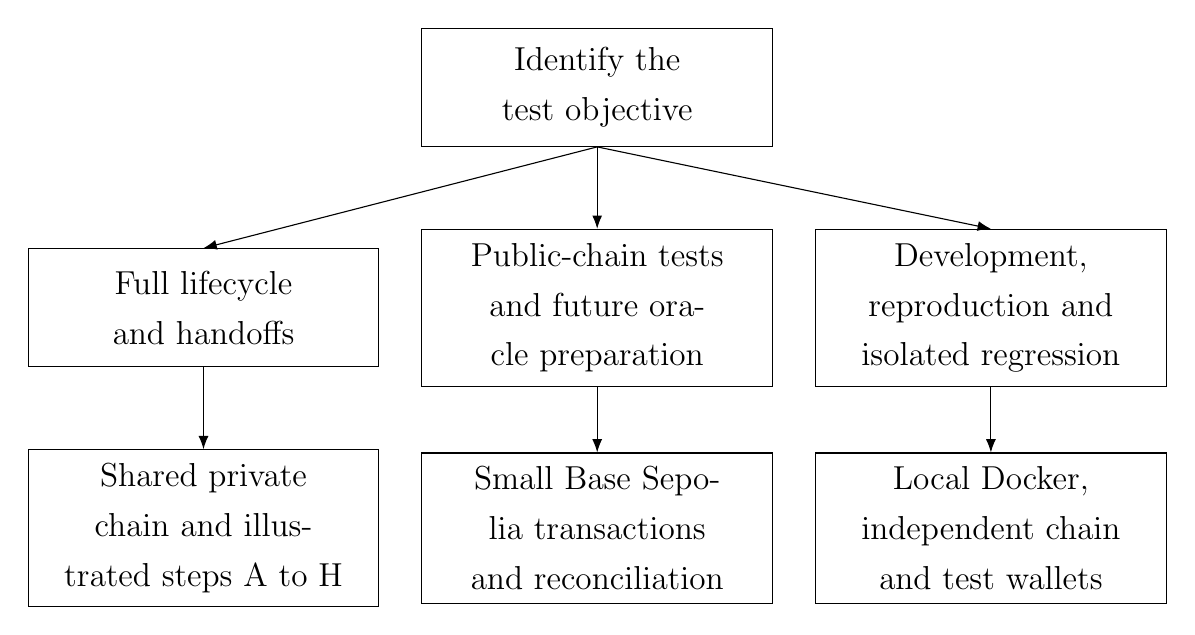
\begin{tikzpicture}[>=Latex,box/.style={draw,align=center,text width=4.1cm,minimum height=1.5cm,inner sep=5pt}]
\node[box] (goal) at (5,0) {Identify the test objective};
\node[box] (private) at (0,-2.8) {Full lifecycle and handoffs};
\node[box] (privateout) at (0,-5.6) {Shared private chain and illustrated steps A to H};
\draw[->] (goal.south)--(private.north);\draw[->] (private.south)--(privateout.north);
\node[box] (base) at (5,-2.8) {Public-chain tests and future oracle preparation};
\node[box] (baseout) at (5,-5.6) {Small Base Sepolia transactions and reconciliation};
\draw[->] (goal.south)--(base.north);\draw[->] (base.south)--(baseout.north);
\node[box] (local) at (10,-2.8) {Development, reproduction and isolated regression};
\node[box] (localout) at (10,-5.6) {Local Docker, independent chain and test wallets};
\draw[->] (goal.south)--(local.north);\draw[->] (local.south)--(localout.north);
\end{tikzpicture}\end{center}
Readers learning the product or checking role handoffs can start with the shared private chain. Use your own local instance for code changes or an issuance from an empty scene. Prepare Base Sepolia test ETH and Circle test USDC when checking public-chain behavior or preparing the later oracle integration. Separate chapters explain each path; the subsequent full workflow illustrations apply to private and local environments according to their current state.

\clearpage\section{Product states and role handoffs}
A product starts as a draft, opens fundraising after approval and issues DRS only on successful settlement. It then enters servicing. Failed fundraising allows refunds, and a live product is reconciled and closed when its rights expire. Contract deployment is distinct from publication, and escrowed subscriptions are distinct from issued shares.

The owner applies, signs the rights agreement and pays monthly bills using their own wallet. The intermediary assesses materials, prepares valuations, organizes issuance and operates the pool. Trustees independently approve offers and pool valuations. Investors complete qualification, subscriptions, claims and exits. Two separate trustees are required for the defined servicing intervention, rather than for every ordinary valuation approval.

\clearpage\begin{landscape}
\subsection{Application, admission and issuance sequence}
Arrows show the order of handoffs. Message signatures and off-chain review are distinct from confirmed blockchain transactions.

\begin{center}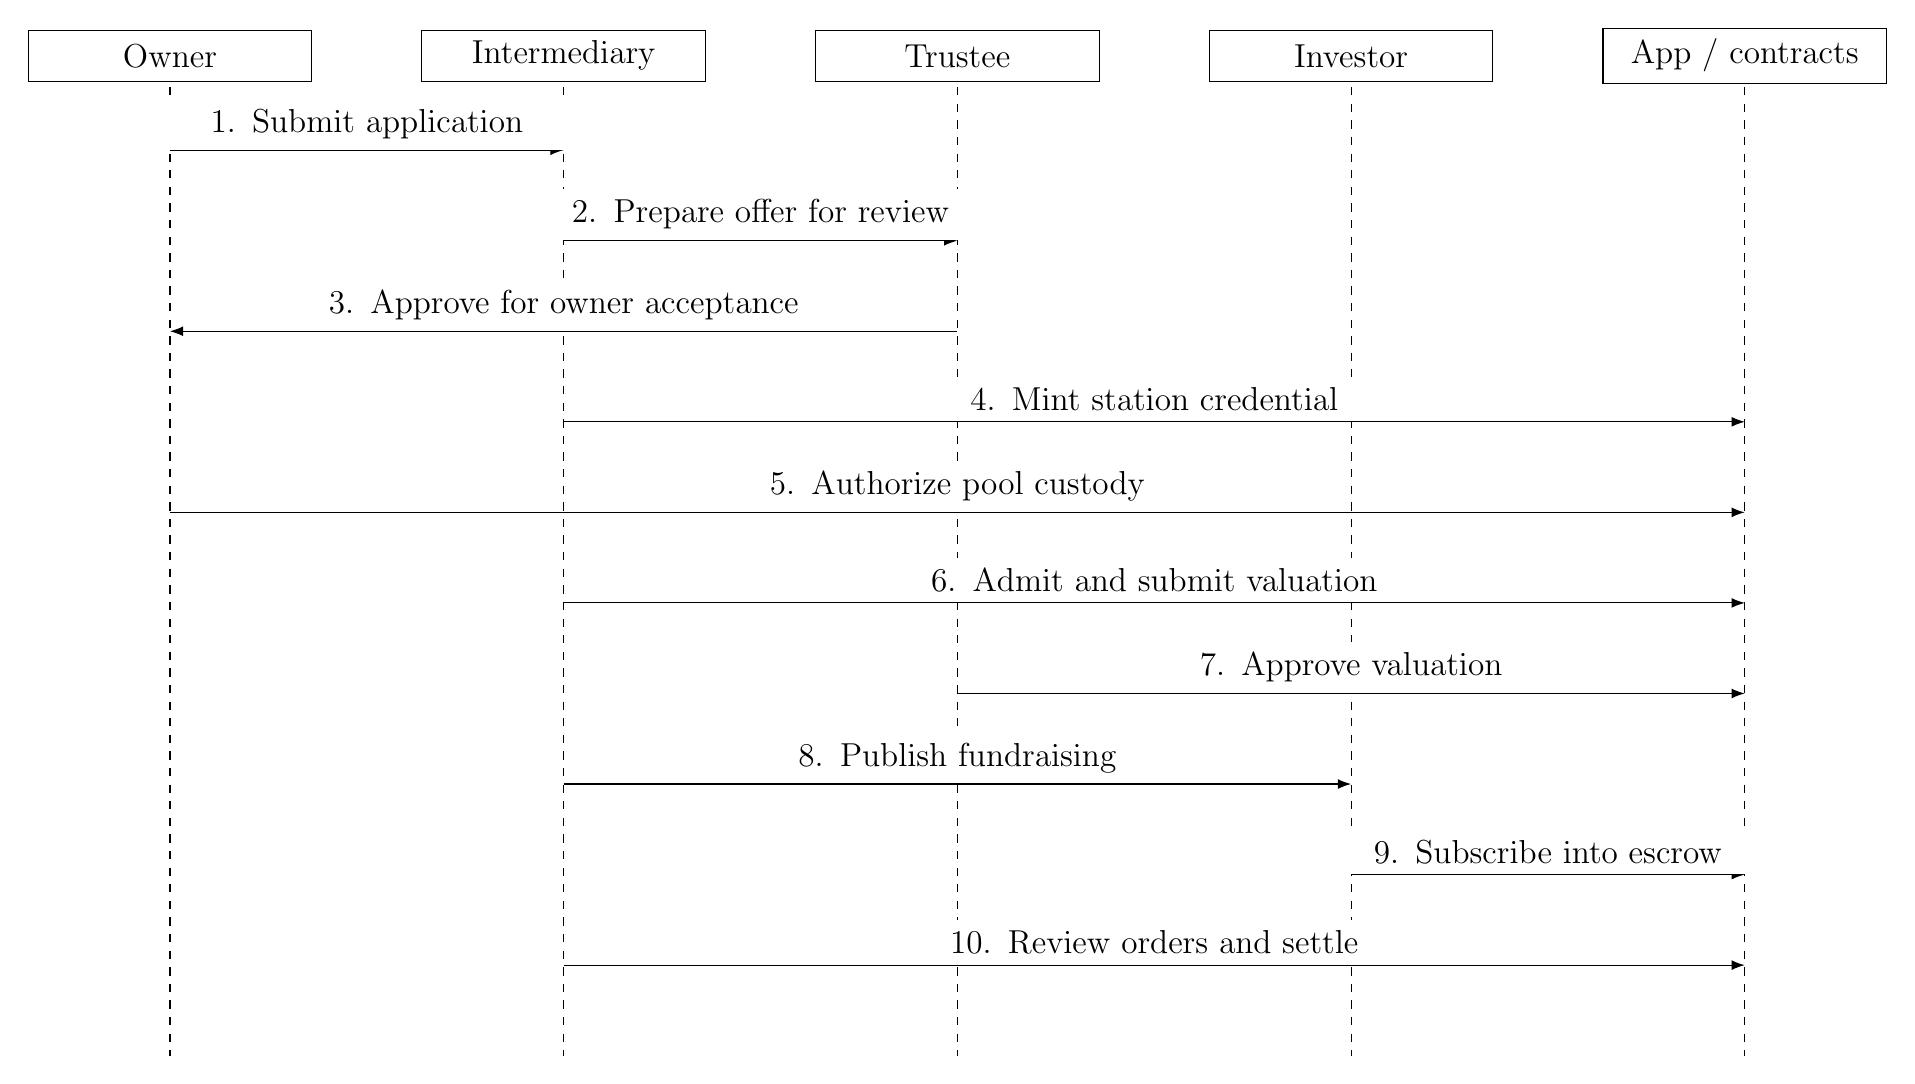
\begin{tikzpicture}[x=1cm,y=1cm,>=Latex]
\node[draw,minimum width=3.6cm,minimum height=.65cm] at (0,0) {Owner};\draw[dashed] (0,-.4)--(0,-12.7);
\node[draw,minimum width=3.6cm,minimum height=.65cm] at (5,0) {Intermediary};\draw[dashed] (5,-.4)--(5,-12.7);
\node[draw,minimum width=3.6cm,minimum height=.65cm] at (10,0) {Trustee};\draw[dashed] (10,-.4)--(10,-12.7);
\node[draw,minimum width=3.6cm,minimum height=.65cm] at (15,0) {Investor};\draw[dashed] (15,-.4)--(15,-12.7);
\node[draw,minimum width=3.6cm,minimum height=.65cm] at (20,0) {App / contracts};\draw[dashed] (20,-.4)--(20,-12.7);
\draw[->] (0,-1.2)--node[above,fill=white,align=center,text width=4.8cm]{1. Submit application}(5,-1.2);
\draw[->] (5,-2.3499999999999996)--node[above,fill=white,align=center,text width=4.8cm]{2. Prepare offer for review}(10,-2.3499999999999996);
\draw[->] (10,-3.5)--node[above,fill=white,align=center,text width=9cm]{3. Approve for owner acceptance}(0,-3.5);
\draw[->] (5,-4.6499999999999995)--node[above,fill=white,align=center,text width=9cm]{4. Mint station credential}(20,-4.6499999999999995);
\draw[->] (0,-5.8)--node[above,fill=white,align=center,text width=9cm]{5. Authorize pool custody}(20,-5.8);
\draw[->] (5,-6.95)--node[above,fill=white,align=center,text width=9cm]{6. Admit and submit valuation}(20,-6.95);
\draw[->] (10,-8.1)--node[above,fill=white,align=center,text width=9cm]{7. Approve valuation}(20,-8.1);
\draw[->] (5,-9.249999999999998)--node[above,fill=white,align=center,text width=9cm]{8. Publish fundraising}(15,-9.249999999999998);
\draw[->] (15,-10.399999999999999)--node[above,fill=white,align=center,text width=4.8cm]{9. Subscribe into escrow}(20,-10.399999999999999);
\draw[->] (5,-11.549999999999999)--node[above,fill=white,align=center,text width=9cm]{10. Review orders and settle}(20,-11.549999999999999);
\end{tikzpicture}\end{center}
\end{landscape}
\clearpage\begin{landscape}
\subsection{Monthly bills and household payment}
Arrows show the order of handoffs. Message signatures and off-chain review are distinct from confirmed blockchain transactions.

\begin{center}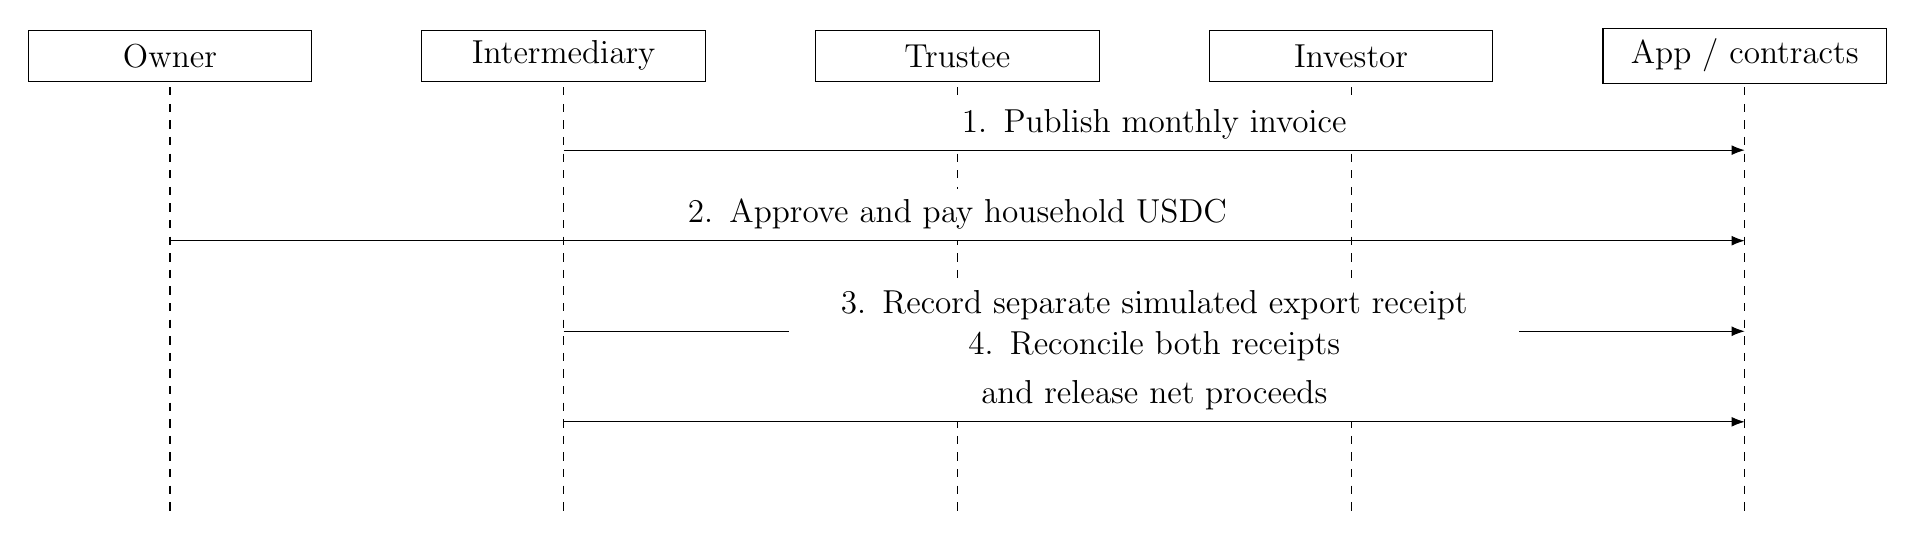
\begin{tikzpicture}[x=1cm,y=1cm,>=Latex]
\node[draw,minimum width=3.6cm,minimum height=.65cm] at (0,0) {Owner};\draw[dashed] (0,-.4)--(0,-5.8);
\node[draw,minimum width=3.6cm,minimum height=.65cm] at (5,0) {Intermediary};\draw[dashed] (5,-.4)--(5,-5.8);
\node[draw,minimum width=3.6cm,minimum height=.65cm] at (10,0) {Trustee};\draw[dashed] (10,-.4)--(10,-5.8);
\node[draw,minimum width=3.6cm,minimum height=.65cm] at (15,0) {Investor};\draw[dashed] (15,-.4)--(15,-5.8);
\node[draw,minimum width=3.6cm,minimum height=.65cm] at (20,0) {App / contracts};\draw[dashed] (20,-.4)--(20,-5.8);
\draw[->] (5,-1.2)--node[above,fill=white,align=center,text width=9cm]{1. Publish monthly invoice}(20,-1.2);
\draw[->] (0,-2.3499999999999996)--node[above,fill=white,align=center,text width=9cm]{2. Approve and pay household USDC}(20,-2.3499999999999996);
\draw[->] (5,-3.5)--node[above,fill=white,align=center,text width=9cm]{3. Record separate simulated export receipt}(20,-3.5);
\draw[->] (5,-4.6499999999999995)--node[above,fill=white,align=center,text width=9cm]{4. Reconcile both receipts and release net proceeds}(20,-4.6499999999999995);
\end{tikzpicture}\end{center}
\end{landscape}
\clearpage\begin{landscape}
\subsection{Monthly valuation and investor handoff}
Arrows show the order of handoffs. Message signatures and off-chain review are distinct from confirmed blockchain transactions.

\begin{center}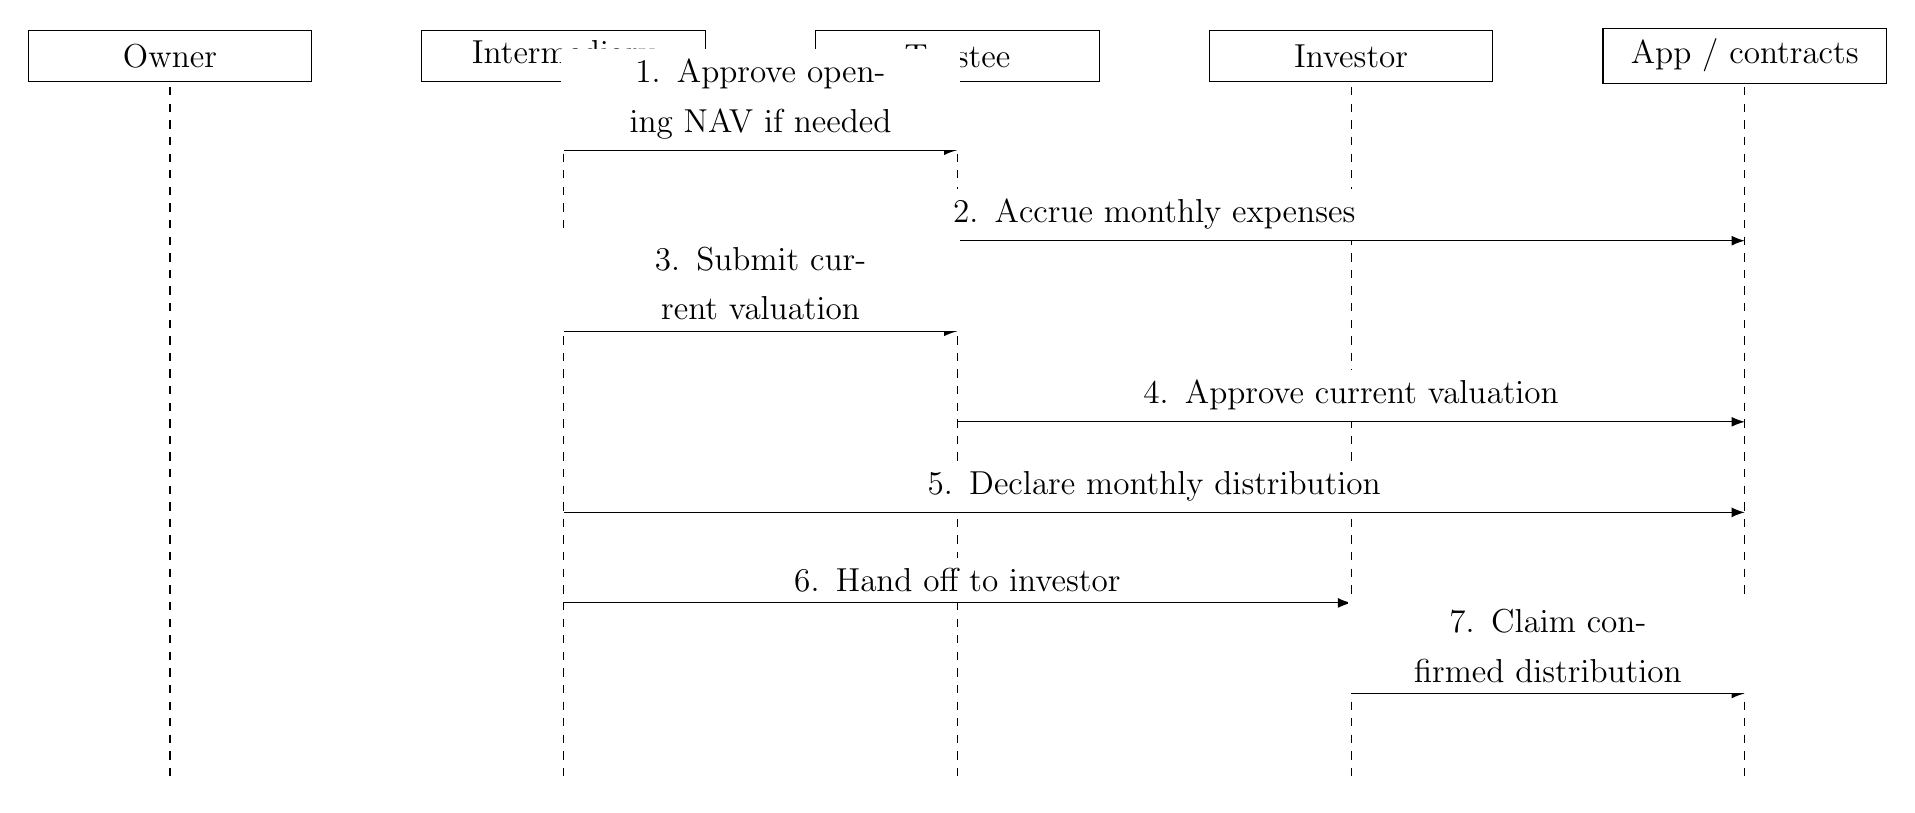
\begin{tikzpicture}[x=1cm,y=1cm,>=Latex]
\node[draw,minimum width=3.6cm,minimum height=.65cm] at (0,0) {Owner};\draw[dashed] (0,-.4)--(0,-9.249999999999998);
\node[draw,minimum width=3.6cm,minimum height=.65cm] at (5,0) {Intermediary};\draw[dashed] (5,-.4)--(5,-9.249999999999998);
\node[draw,minimum width=3.6cm,minimum height=.65cm] at (10,0) {Trustee};\draw[dashed] (10,-.4)--(10,-9.249999999999998);
\node[draw,minimum width=3.6cm,minimum height=.65cm] at (15,0) {Investor};\draw[dashed] (15,-.4)--(15,-9.249999999999998);
\node[draw,minimum width=3.6cm,minimum height=.65cm] at (20,0) {App / contracts};\draw[dashed] (20,-.4)--(20,-9.249999999999998);
\draw[->] (5,-1.2)--node[above,fill=white,align=center,text width=4.8cm]{1. Approve opening NAV if needed}(10,-1.2);
\draw[->] (5,-2.3499999999999996)--node[above,fill=white,align=center,text width=9cm]{2. Accrue monthly expenses}(20,-2.3499999999999996);
\draw[->] (5,-3.5)--node[above,fill=white,align=center,text width=4.8cm]{3. Submit current valuation}(10,-3.5);
\draw[->] (10,-4.6499999999999995)--node[above,fill=white,align=center,text width=9cm]{4. Approve current valuation}(20,-4.6499999999999995);
\draw[->] (5,-5.8)--node[above,fill=white,align=center,text width=9cm]{5. Declare monthly distribution}(20,-5.8);
\draw[->] (5,-6.95)--node[above,fill=white,align=center,text width=9cm]{6. Hand off to investor}(15,-6.95);
\draw[->] (15,-8.1)--node[above,fill=white,align=center,text width=4.8cm]{7. Claim confirmed distribution}(20,-8.1);
\end{tikzpicture}\end{center}
\end{landscape}
\clearpage\begin{landscape}
\section{System composition and architecture}
\subsection{System composition}
The homepage remains readable independently. The application, RPC and explorer run in an isolated Docker environment on the Mac and are exposed through HTTPS tunnels.

\begin{center}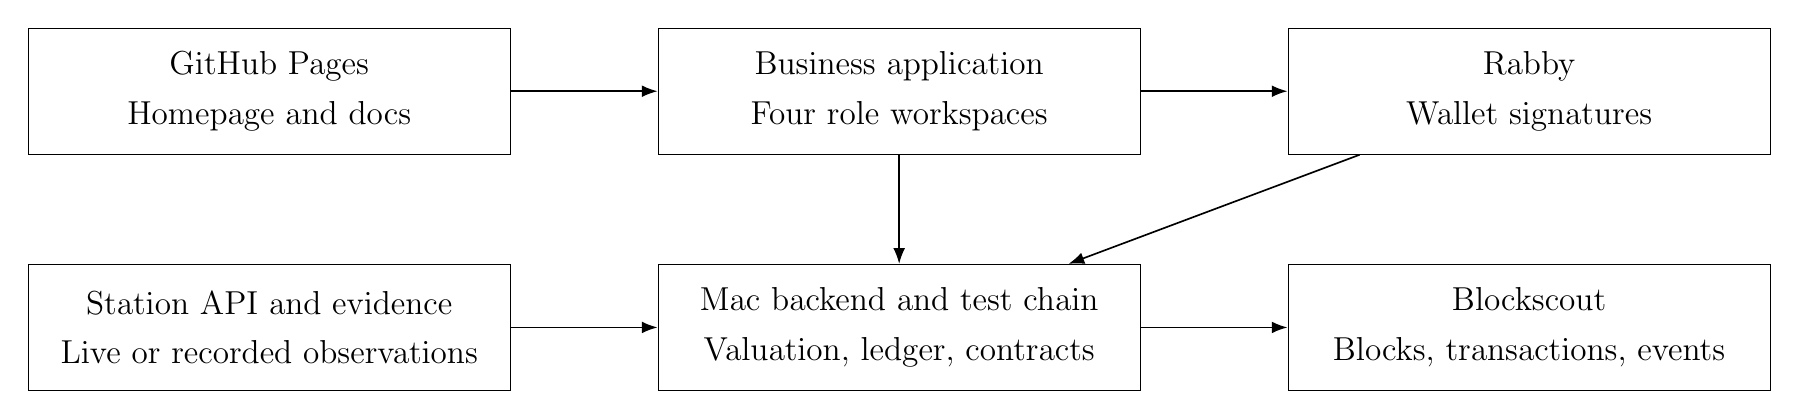
\begin{tikzpicture}[x=1cm,y=1cm,>=Latex,box/.style={draw,align=center,text width=5.7cm,minimum height=1.6cm,inner sep=6pt},arrow/.style={->,line width=.6pt}]
\node[box] (a) at (0,0) {GitHub Pages\\Homepage and docs};
\node[box] (b) at (8,0) {Business application\\Four role workspaces};
\node[box] (c) at (16,0) {Rabby\\Wallet signatures};
\node[box] (d) at (0,-3) {Station API and evidence\\Live or recorded observations};
\node[box] (e) at (8,-3) {Mac backend and test chain\\Valuation, ledger, contracts};
\node[box] (f) at (16,-3) {Blockscout\\Blocks, transactions, events};
\draw[arrow] (a) -- (b);
\draw[arrow] (b) -- (c);
\draw[arrow] (b) -- (e);
\draw[arrow] (d) -- (e);
\draw[arrow] (c) -- (e);
\draw[arrow] (e) -- (f);
\end{tikzpicture}\end{center}
\end{landscape}
\clearpage\begin{landscape}
\subsection{Business architecture}
Discounted owner electricity payments and eligible export receipts fund the rights. The pool pays the agreed purchase price and handles expenses, distributions and exits without acquiring equipment ownership.

\begin{center}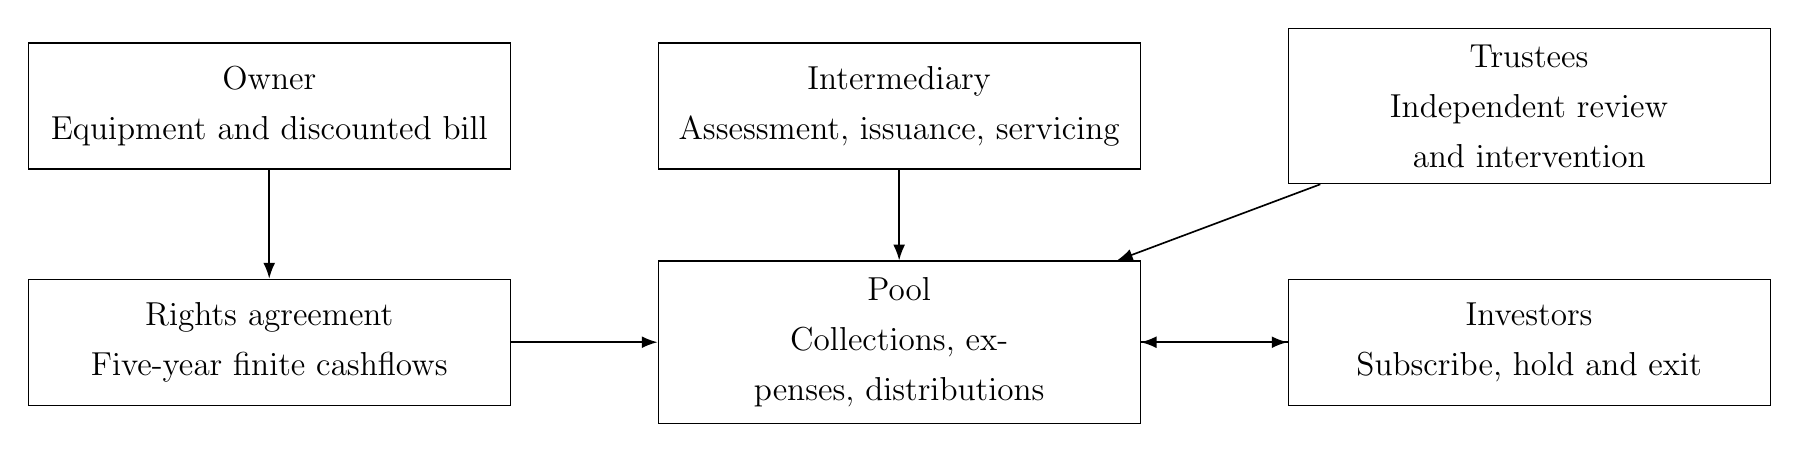
\begin{tikzpicture}[x=1cm,y=1cm,>=Latex,box/.style={draw,align=center,text width=5.7cm,minimum height=1.6cm,inner sep=6pt},arrow/.style={->,line width=.6pt}]
\node[box] (a) at (0,0) {Owner\\Equipment and discounted bill};
\node[box] (b) at (8,0) {Intermediary\\Assessment, issuance, servicing};
\node[box] (c) at (16,0) {Trustees\\Independent review and intervention};
\node[box] (d) at (0,-3) {Rights agreement\\Five-year finite cashflows};
\node[box] (e) at (8,-3) {Pool\\Collections, expenses, distributions};
\node[box] (f) at (16,-3) {Investors\\Subscribe, hold and exit};
\draw[arrow] (a) -- (d);
\draw[arrow] (d) -- (e);
\draw[arrow] (b) -- (e);
\draw[arrow] (c) -- (e);
\draw[arrow] (f) -- (e);
\draw[arrow] (e) -- (f);
\end{tikzpicture}\end{center}
\end{landscape}
\clearpage\begin{landscape}
\subsection{Data architecture}
Observed energy, modeled values, review status and chain confirmation are recorded separately. Collection is not another revenue recognition, and anchoring a digest does not publish the underlying raw evidence.

\begin{center}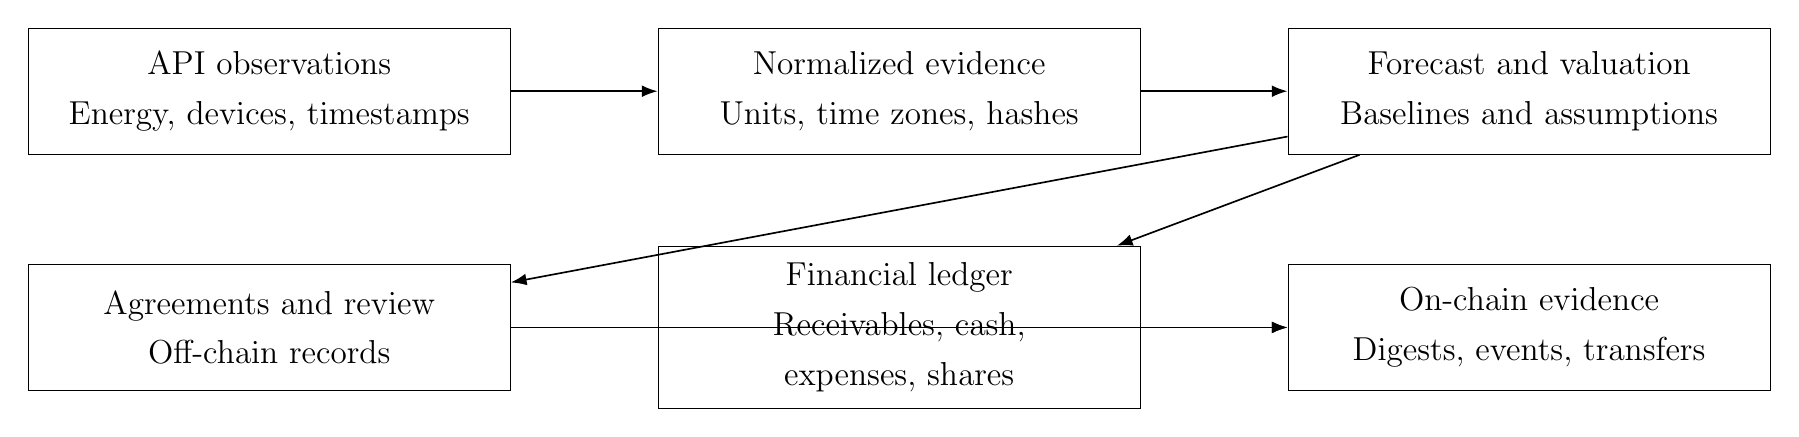
\begin{tikzpicture}[x=1cm,y=1cm,>=Latex,box/.style={draw,align=center,text width=5.7cm,minimum height=1.6cm,inner sep=6pt},arrow/.style={->,line width=.6pt}]
\node[box] (a) at (0,0) {API observations\\Energy, devices, timestamps};
\node[box] (b) at (8,0) {Normalized evidence\\Units, time zones, hashes};
\node[box] (c) at (16,0) {Forecast and valuation\\Baselines and assumptions};
\node[box] (d) at (0,-3) {Agreements and review\\Off-chain records};
\node[box] (e) at (8,-3) {Financial ledger\\Receivables, cash, expenses, shares};
\node[box] (f) at (16,-3) {On-chain evidence\\Digests, events, transfers};
\draw[arrow] (a) -- (b);
\draw[arrow] (b) -- (c);
\draw[arrow] (c) -- (d);
\draw[arrow] (d) -- (f);
\draw[arrow] (c) -- (e);
\draw[arrow] (e) -- (f);
\end{tikzpicture}\end{center}
\end{landscape}
\clearpage\begin{landscape}
\subsection{Functional architecture}
Workspaces show the operations permitted for each role. Guidance derives from actual state, and choosing a role does not grant approval, payment or signing authority.

\begin{center}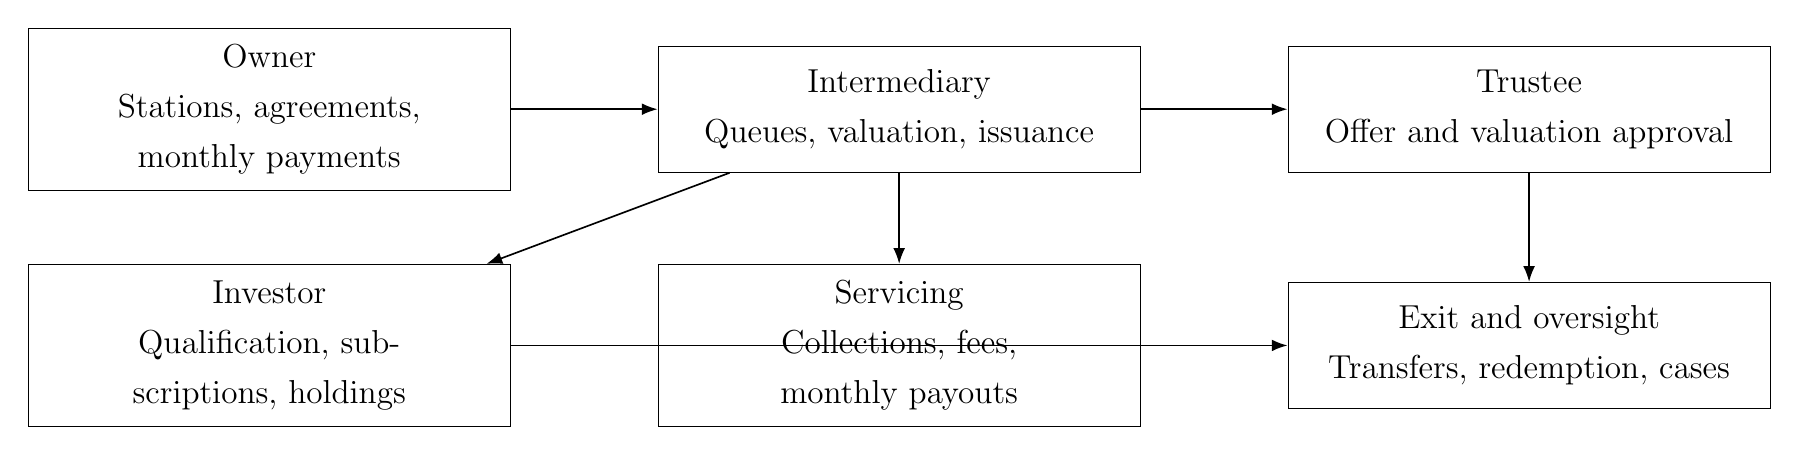
\begin{tikzpicture}[x=1cm,y=1cm,>=Latex,box/.style={draw,align=center,text width=5.7cm,minimum height=1.6cm,inner sep=6pt},arrow/.style={->,line width=.6pt}]
\node[box] (a) at (0,0) {Owner\\Stations, agreements, monthly payments};
\node[box] (b) at (8,0) {Intermediary\\Queues, valuation, issuance};
\node[box] (c) at (16,0) {Trustee\\Offer and valuation approval};
\node[box] (d) at (0,-3) {Investor\\Qualification, subscriptions, holdings};
\node[box] (e) at (8,-3) {Servicing\\Collections, fees, monthly payouts};
\node[box] (f) at (16,-3) {Exit and oversight\\Transfers, redemption, cases};
\draw[arrow] (a) -- (b);
\draw[arrow] (b) -- (c);
\draw[arrow] (b) -- (d);
\draw[arrow] (b) -- (e);
\draw[arrow] (d) -- (f);
\draw[arrow] (c) -- (f);
\end{tikzpicture}\end{center}
\end{landscape}
\clearpage\begin{landscape}
\subsection{Technical architecture}
Wallets sign on the client. The backend checks sender, target, method, arguments, receipt and events before advancing workflow state. The public RPC rejects reset, impersonation and balance-editing methods.

\begin{center}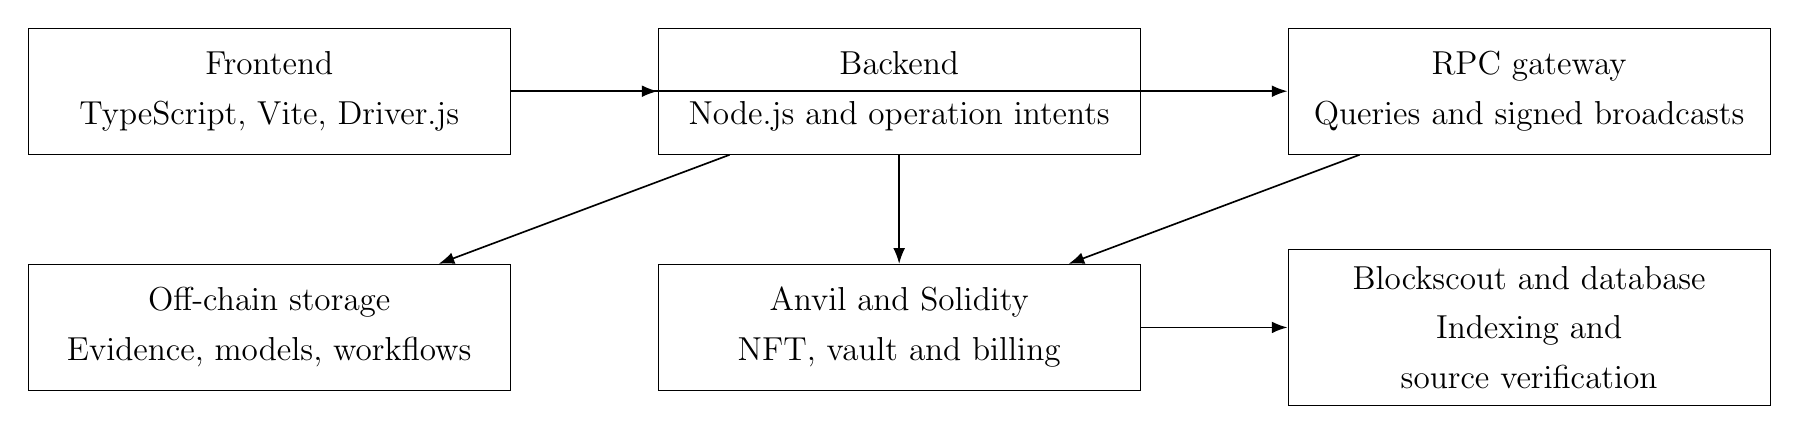
\begin{tikzpicture}[x=1cm,y=1cm,>=Latex,box/.style={draw,align=center,text width=5.7cm,minimum height=1.6cm,inner sep=6pt},arrow/.style={->,line width=.6pt}]
\node[box] (a) at (0,0) {Frontend\\TypeScript, Vite, Driver.js};
\node[box] (b) at (8,0) {Backend\\Node.js and operation intents};
\node[box] (c) at (16,0) {RPC gateway\\Queries and signed broadcasts};
\node[box] (d) at (0,-3) {Off-chain storage\\Evidence, models, workflows};
\node[box] (e) at (8,-3) {Anvil and Solidity\\NFT, vault and billing};
\node[box] (f) at (16,-3) {Blockscout and database\\Indexing and source verification};
\draw[arrow] (a) -- (b);
\draw[arrow] (a) -- (c);
\draw[arrow] (b) -- (d);
\draw[arrow] (b) -- (e);
\draw[arrow] (c) -- (e);
\draw[arrow] (e) -- (f);
\end{tikzpicture}\end{center}
\end{landscape}
\clearpage\section{Wallets and test accounts}
Install the browser extension through Rabby’s official website. Choose an existing address and private-key import, then verify the resulting full address. Enter private keys only inside the wallet extension. The business website never needs them.

\url{https://rabby.io/}\par
\begin{center}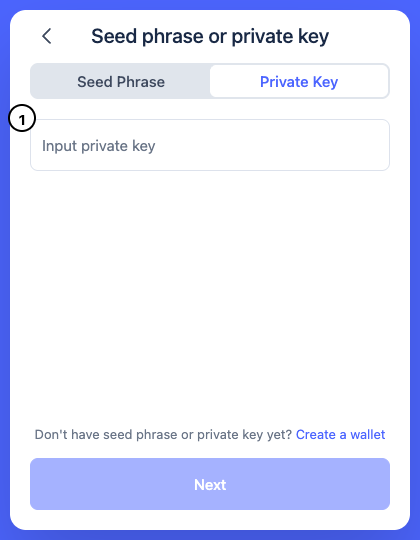
\includegraphics[width=\linewidth,height=.42\textheight,keepaspectratio]{assets/wallet-import-3-crop.png}\par Marker 1 identifies the private-key field inside the wallet extension. The illustrated field is empty.\end{center}
This release preserves the public owner, intermediary and two trustee addresses. Role bindings are not generated by clicking a role button. An ordinary wallet may apply as an investor. Investor A/B and trustee A/B use separate accounts for a full walkthrough.

The two trustees use the same login role but different wallets. A servicing case requires 30\% support under its fixed snapshot and approval from two distinct trustees before changing the demo collection recipient. Repeating approval with one address does not replace the second trustee.

\clearpage\begin{landscape}
\subsection{Role accounts 1}
\textbf{Owner}\par
\nolinkurl{0xadC4920e9036dadC146ba1aF84fb1475C612E15b}\par
The demo operator supplies the private key through an internal channel. It is excluded from this source document.

\textbf{Intermediary}\par
\nolinkurl{0xcee71e610f50435B8C9B0B25d3D322a5E184423a}\par
The demo operator supplies the private key through an internal channel. It is excluded from this source document.

\end{landscape}
\clearpage\begin{landscape}
\subsection{Role accounts 2}
\textbf{Investor A}\par
\nolinkurl{0x34cAACf0E56129F461afA460cDa3B220a3bfe2F2}\par
The demo operator supplies the private key through an internal channel. It is excluded from this source document.

\textbf{Investor B}\par
\nolinkurl{0xcC245B1140F25b91BD8C13B05d9516A85da75605}\par
The demo operator supplies the private key through an internal channel. It is excluded from this source document.

\end{landscape}
\clearpage\begin{landscape}
\subsection{Role accounts 3}
\textbf{Trustee A}\par
\nolinkurl{0x2641feCc09b01C7C482F51deDB28372daa41326a}\par
The demo operator supplies the private key through an internal channel. It is excluded from this source document.

\textbf{Trustee B}\par
\nolinkurl{0xfcf63f6E1100C4dD1bd0630C358848d990E33e64}\par
The demo operator supplies the private key through an internal channel. It is excluded from this source document.

\end{landscape}
\clearpage\section{Website, network and blockchain explorer}
\subsection{Unified public entry}
\url{https://reuters-romance-arranged-bloggers.trycloudflare.com/}\par
The addresses below were checked on 30 October 2026. The unified entry provides network selection for the private demonstration and Base Sepolia. Cloudflare temporary domains can change. If a bookmarked direct address stops working, open the public homepage and click Launch App to obtain the current entry.

\subsection{Public homepage}
\url{https://mengzhon001.github.io/deye-rwa-demo}\par
\subsection{Business application}
\url{https://reuters-romance-arranged-bloggers.trycloudflare.com/networks/private/app/}\par
\subsection{Blockchain explorer}
\url{https://quizzes-faces-simplified-discuss.trycloudflare.com}\par
\subsection{Wallet RPC}
\url{https://mazda-lopez-stevens-pittsburgh.trycloudflare.com}\par
The test network Chain ID is 20261008 and its gas token is DETH. Check the current RPC when adding the network. A tunnel change requires a new RPC URL but does not change the chain, accounts or existing balances. The address 127.0.0.1 points to the reader’s own computer and is not a remote access address.

Click a confirmed transaction hash to open its Blockscout page. Alternatively, paste a full hash, account or contract into the explorer search field. Check status, sender, target and block, followed by token transfers and events. Login and agreement message signatures are off-chain and do not create transaction records.

\subsection{Network selection and session isolation}
One business website now provides access to the private demonstration and Base Sepolia. Select a network on the GitHub homepage and click Launch App. The network button in the upper-right corner shows the current chain. Its menu explains each chain and its Chain ID. Network selection is also available in the sign-in dialog, before authentication.

After the wallet signature is verified, the role workspace and navigation appear first. Product metadata, wallet balances and saved records load independently. Transaction controls remain unavailable until the required business state is loaded, and a pending amount does not mean zero. An unavailable section can be retried separately. If business-state loading fails, sign-in is retained without repeatedly connecting or signing again.

To switch, confirm the destination network in Rabby and sign in again with the intended role. Role addresses remain unchanged, while sessions, products, pending operations and page selections are isolated by chain. Switching does not convert or bridge private-chain mUSDC into Circle USDC. Reconcile any pending operation on its original page or in the transaction log before switching. A rejected wallet request or unavailable destination leaves the application on its original network.

\begin{center}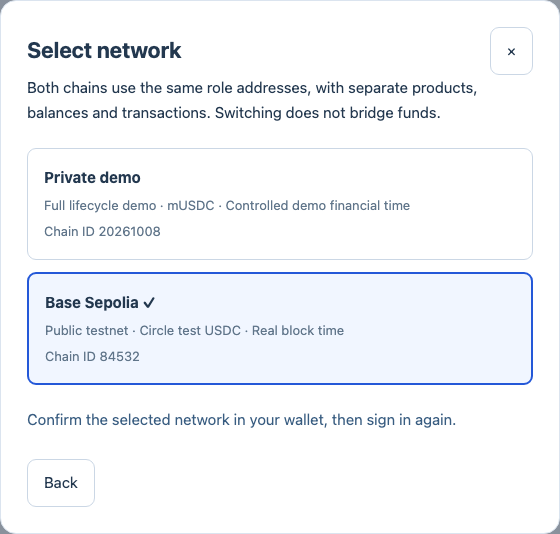
\includegraphics[width=\linewidth,height=.42\textheight,keepaspectratio]{assets/network-menu.en.png}\par Network selection in the unified application. Select the chain, verify it in the wallet and sign in again.\end{center}
\clearpage\section{Full lifecycle testing on the private demonstration}
\subsection{Purpose and prerequisites}
The shared private demonstration checks the complete handoff of the revenue-rights business between roles. It uses Anvil, demo mUSDC and its own Blockscout. Authorized intermediary time advancement allows monthly operations, the six-month lock, quarterly redemption and expiry to be exercised without waiting through the real calendar. Advancing time creates no station telemetry and does not replace invoices, payments, approvals or distribution transactions.

Obtain the role test accounts from the operator and agree which product the group will use. A full walkthrough requires an owner, intermediary, investors A/B and trustees A/B. An investor-only check can use a prepared product that is published and still fundraising, without repeating the application and issuance preparation. If the product is already active, primary fundraising subscriptions are closed; select another fundraising product or ask the operator to prepare a new scene.

\subsection{Entry and network confirmation}
\url{https://reuters-romance-arranged-bloggers.trycloudflare.com/networks/private/app/}\par
Click Launch App on the public homepage and select Private demo in the upper-right network menu. Verify Chain ID 20261008 in Rabby, select the intended role and sign in. Check the product name and vault address. Wallet funds, escrowed orders and issued DRS are separate records. Claiming demo funds increases the wallet balance but does not submit a subscription.

\subsection{Direct investor testing}
Choose a fundraising product, inspect its cashflow timeline and risks, and submit the eligibility declarations. After intermediary approval, obtain demo funds, enter an amount within the remaining capacity, approve mUSDC and confirm the subscription transaction. The intermediary reviews the current cumulative order. Additional subscriptions are allowed while fundraising and capacity permit, and each addition requires another review.

To check refunds, the original investor can cancel before settlement and recover the entire cumulative escrow. To continue to holdings and distributions, cover the displayed settlement shortfall and have the intermediary review and settle. The contract retains the agreed 10\% cash automatically; there is no separate reserve-transfer step. Until settlement completes, escrow must not be treated as issued shares.

\clearpage
\subsection{Lifecycle and illustrated-step index}
The table organizes the full walkthrough by business state. Confirm both the page result and corresponding chain record before handing off to the next role. The identifiers link to the annotated illustrations later in the manual. Investor testing on a prepared product starts with group D, while an empty scene starts with group B.

\begin{longtable}{L{2.8cm}L{4.6cm}L{5.1cm}L{1.7cm}}\toprule Stage & Participant and action & Result to confirm & Figures\\\midrule\endhead
Application and agreement & Owner applies; intermediary reviews and prices; trustee approves; owner accepts and signs. & Agreement, valuation and station evidence match. & \hyperref[step:B3]{B3} / \hyperref[step:B10]{B10}\\\addlinespace
Admission and publication & Intermediary mints; owner authorizes; intermediary admits and prepares NAV; trustee approves before publication. & Fundraising opens with reconciled custody and issuance terms. & \hyperref[step:C1]{C1} / \hyperref[step:C6]{C6}\\\addlinespace
Subscription and settlement & Investors obtain eligibility and subscribe; intermediary reviews and settles. & Escrow pays for rights, cash is retained and investors receive DRS. & \hyperref[step:D3]{D3} / \hyperref[step:D8]{D8}\\\addlinespace
Monthly servicing & Intermediary bills; owner pays; intermediary reconciles export and receipts; trustee approves NAV. & Both receipt sources, expenses and approved NAV are recorded separately. & \hyperref[step:E1]{E1} / \hyperref[step:E5]{E5}\\\addlinespace
Declaration and claim & Intermediary declares the monthly distribution; investors switch to their own wallets and claim. & Declared, claimable and paid amounts reconcile with USDC transfers. & \hyperref[step:E6]{E6} / \hyperref[step:E7]{E7}\\\addlinespace
Transfer and redemption & Participants and intermediary act after lock and notice conditions are met. & Shares, payments, partial fills and remaining requests agree. & \hyperref[step:F1]{F1}\\\addlinespace
Servicing and closure & Obtain snapshot support and two trustee approvals where required, then reconcile expiry. & Receivables and liabilities are reconciled, with final distribution and credential release. & \hyperref[step:G1]{G1} / \hyperref[step:H1]{H1}\\\addlinespace
\bottomrule\end{longtable}
\subsection{Clock advancement, shared state and evidence}
When waiting for a cutoff, the intermediary opens Product operations, expands Demo tools: financial time, selects the next monthly fee cutoff and confirms. Where supported, the guide locates the same shortcut. Complete each month's billing, receipts, expenses and valuation approval before moving to the next month. Skipping dates does not complete the missing accounting.

Products in the shared environment use the same chain clock. Advancing it can expire another product's fundraising or valuation, so coordinate through one operator. The operator should also control resets and preparation of new sample products. Record the product and role addresses, key hashes, business identifiers, expected outcomes and actual results. Do not record off-chain review as an on-chain transaction.

\clearpage\section{Base Sepolia public-chain testing}
The original public demonstration remains the environment for the full accelerated lifecycle. Base Sepolia is a separate environment for public-chain contracts and wallet transactions. Role addresses are shared, but contracts, balances and workflow records are independent. The complete lifecycle screenshots later in this manual illustrate the private-chain demonstration. Public-chain testing follows the real-time and funding restrictions in this section.

\subsection{Test objectives and later oracle integration}
Base Sepolia checks whether the business code handles wallet signatures, gas, Circle USDC approvals and transfers, contract calls, event reads and recovery on a real public chain. It also provides the foundation for later oracle integration, where report receivers, report digests, billing-period binding, permissions and failure handling can be tested on the same public test chain without disturbing the private-chain demonstration.

The current deployment has no oracle integration. Present tests validate public-chain transactions and the existing report workflow; they do not establish independent oracle certification of station data. The later implementation must add off-chain retrieval and validation, report signatures or attestations, and on-chain receipt and enforcement, followed by deployment and testing of the affected components. An oracle attestation does not itself prove household payment; USDC receipts still require separate transaction reconciliation.

\subsection{Entry and network configuration}
Public-chain application\par\url{https://reuters-romance-arranged-bloggers.trycloudflare.com/networks/base-sepolia/app/}\par
Public-chain explorer\par\url{https://base-sepolia.blockscout.com}\par
Wallet RPC\par\url{https://sepolia.base.org}\par
The Chain ID is 84532, gas is paid in test ETH, and payments use Circle test USDC. The homepage and application share one network-selection entry. Select Base Sepolia and verify the wallet network before signing in.

\nolinkurl{0x036CbD53842c5426634e7929541eC2318f3dCF7e}\par
The address above identifies the official Circle test USDC used here, with six decimals. It is separate from private-chain mUSDC. Test tokens have no monetary value, and balances on another chain cannot pay for subscriptions here.

\subsection{Environment components and data flow}
\begin{center}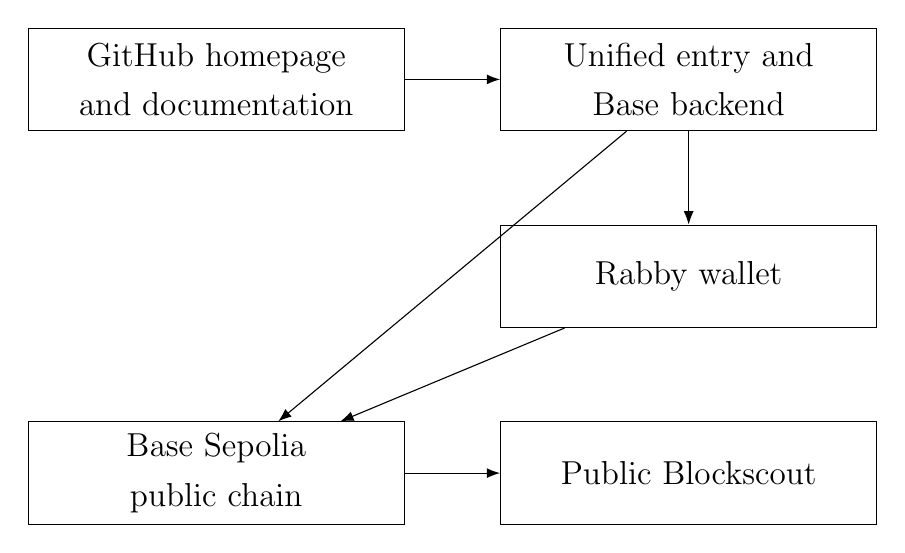
\begin{tikzpicture}[>=Latex,node distance=1cm,box/.style={draw,align=center,text width=4.5cm,minimum height=1.3cm}]
\node[box] (web) at (0,0) {GitHub homepage and documentation};
\node[box] (app) at (6,0) {Unified entry and Base backend};
\node[box] (wallet) at (6,-2.5) {Rabby wallet};
\node[box] (chain) at (0,-5) {Base Sepolia public chain};
\node[box] (explorer) at (6,-5) {Public Blockscout};
\draw[->] (web)--(app);
\draw[->] (app)--(wallet);
\draw[->] (wallet)--(chain);
\draw[->] (app)--(chain);
\draw[->] (chain)--(explorer);
\end{tikzpicture}\end{center}
The shared HTTPS application routes network-specific paths to the corresponding independent backend. The wallet signs transactions for Base Sepolia, the backend checks receipts and events, and the public explorer indexes the results. This environment does not run Anvil or depend on the private-chain RPC tunnel.

\subsection{Funding and subscription steps}
Open the official faucets from the test-funds entry, select Base Sepolia and request test ETH and Circle test USDC for the current role address. Providers may require login or limit claims. The application cannot mint Circle USDC. After confirmation, return and refresh the balance. Enter private keys only inside the wallet extension, never in a faucet or the application.

\url{https://portal.cdp.coinbase.com/products/faucet}\par\url{https://faucet.circle.com/}\par
Select a fundraising product and apply for eligibility. After intermediary approval, enter an amount, approve the corresponding USDC allowance and confirm the subscription transaction. Additional subscriptions are allowed while fundraising remains open, and the intermediary reviews the new accumulated amount. Cancellation before settlement refunds the full accumulated escrow for that address. Escrow does not mean DRS has been issued.

Settlement still requires a current valuation, order approvals, the fundraising threshold and sufficient purchase funding and reserve. The contract automatically retains 10\%; no separate reserve transfer is needed. Small test balances support approvals, subscriptions, review and refunds, but do not establish that a larger funded settlement has completed.

\subsection{Public-chain checks and completion criteria}
Start with one investor account and test sign-in, eligibility, USDC approval, a small subscription and its refund. Then check the intermediary and trustee permissions using their own accounts. Verify the network and balance before each transaction, and reconcile its receipt, events and token transfers in the public explorer. While fundraising is open, add a subscription and check that the intermediary reviews the latest cumulative amount. Retain and reconfirm the original hash when a submitted transaction is slow to appear rather than paying again.

This round is complete when actual transaction amounts agree with business records, wrong wallets and networks are rejected, and records recover after refresh or restart. If settlement funding or the real monthly cutoff has not been reached, record settlement, billing and distribution as not executed in this round and explain why. Small test balances and a short observation window do not amount to lifecycle acceptance; use the private demonstration or your own local instance for that path.

\subsection{Real time and testing scope}
The application cannot advance public-chain time. Monthly billing requires a settled product and the end of the relevant service period. The six-month transfer lock, redemption notice period and expiry remain unchanged. Reset and time-advance controls are therefore unavailable. Use the original public private-chain environment for the complete accelerated lifecycle.

Household monthly payments use Circle test USDC. Grid-export receipts remain a separately disclosed economic simulation, funded from a prefunded independent treasury. Station observations use fixed recorded evidence; tariffs and future cashflows remain modeling assumptions. No oracle is added by this deployment, so anchoring a report does not independently validate API data.

\clearpage
\subsection{Transaction checks and recovery}
After submission, use the hash to check the sender, destination, method, events and USDC transfers in the public explorer. The wallet and backend RPC may see the same transaction at different times. Retain the original hash and retry confirmation rather than paying again. Explorer indexing can lag without a transaction having failed.

Station credential\par\nolinkurl{0xf17FFEAb245CebCd260a2E6aFAe90A43F2749176}\par
Revenue-rights vault\par\nolinkurl{0xB84F6E2EB3b9e63bBE447190dF268c49D617A445}\par
Monthly billing contract\par\nolinkurl{0xa2748E730069A38913b5E2e09a45C5aB546a0908}\par
\clearpage\begin{landscape}
\begin{center}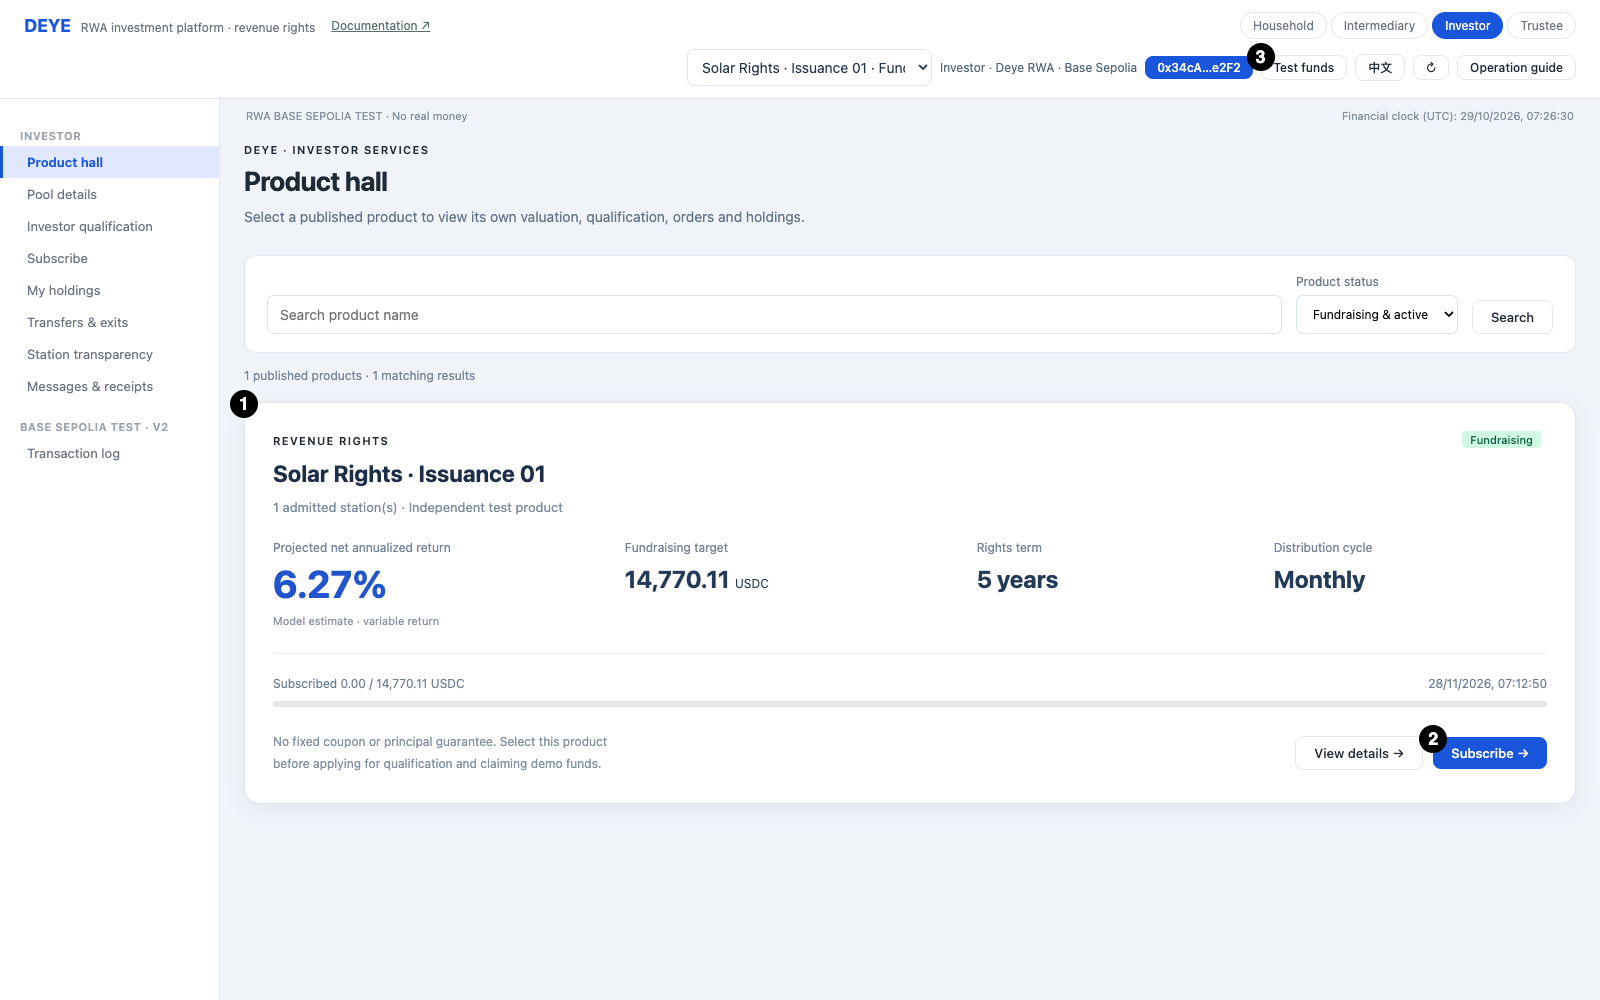
\includegraphics[width=\linewidth,height=.90\textheight,keepaspectratio]{assets/base-product.en.png}\par Public-chain product and network. Markers identify the product, subscription navigation and test-funds entry.\end{center}
\end{landscape}
\clearpage\begin{landscape}
\begin{center}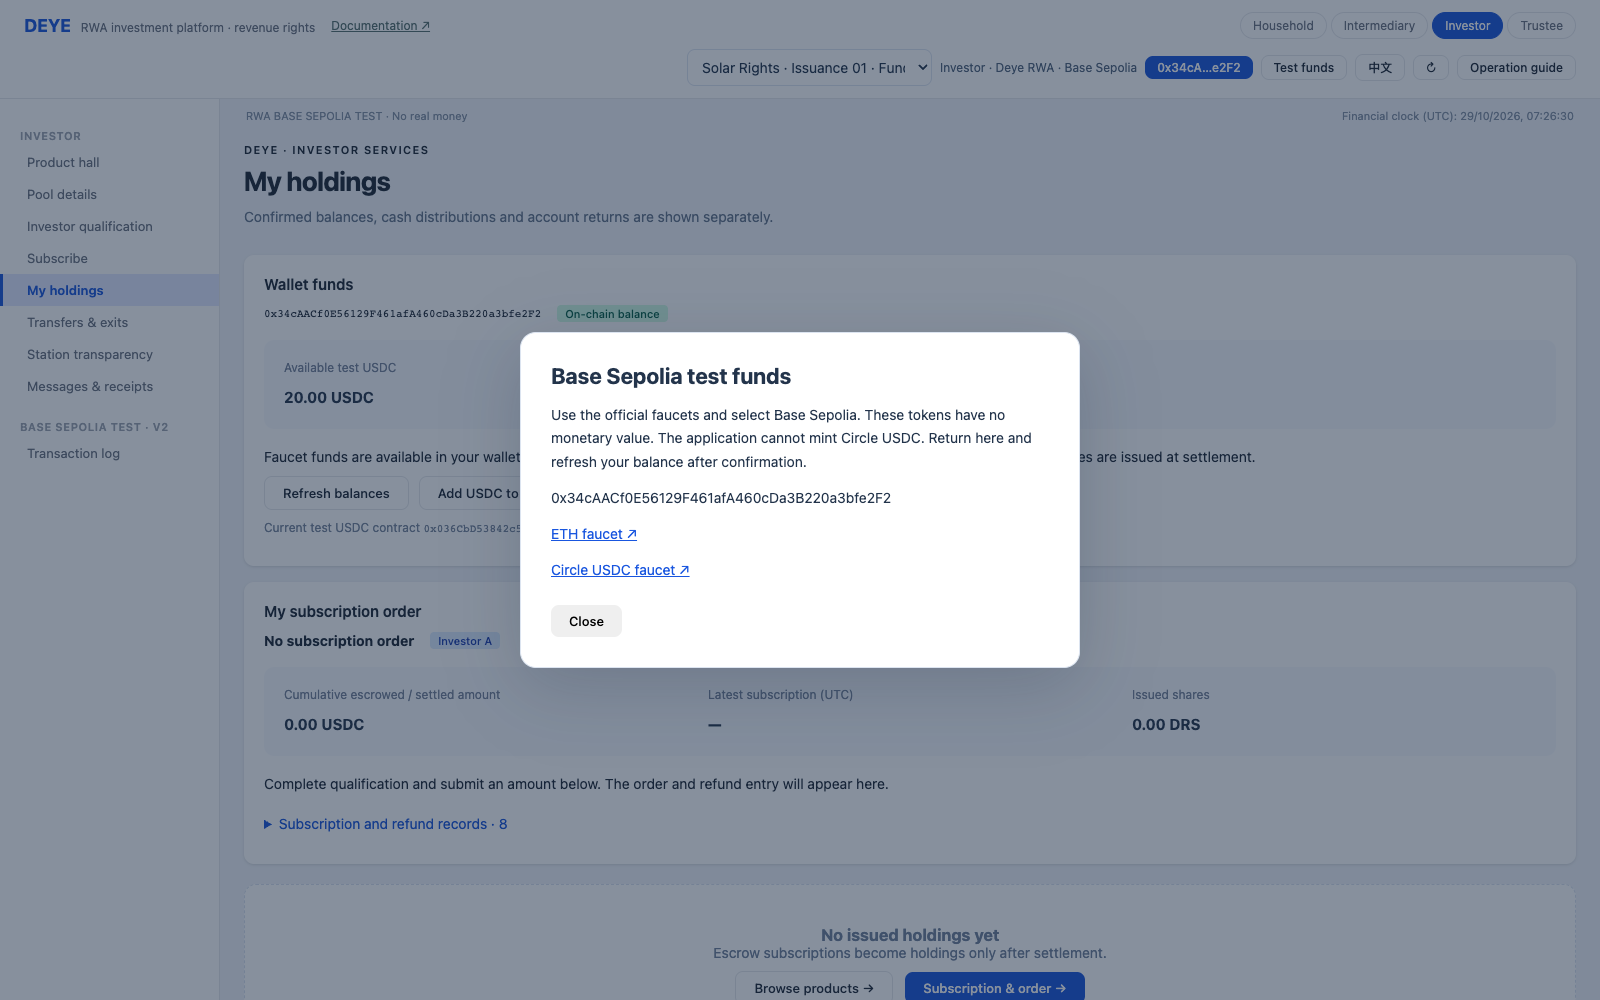
\includegraphics[width=\linewidth,height=.90\textheight,keepaspectratio]{assets/base-wallet.en.png}\par Wallet balances and official-faucet instructions. The backend does not mint Circle USDC.\end{center}
\end{landscape}
\clearpage\section{Local deployment and independent testing}
\subsection{Purpose and default environment}
A local deployment lets developers reproduce issues, change the model and contracts, validate the interface and repeat a walkthrough from an empty scene. It needs no public tunnel and does not depend on the demonstration operator's Mac staying online. The commands below assume a fresh clone in an independent directory, not a working directory already hosting the shared demonstration.

The default Compose project is deye-rwa-platform and its Chain ID is 20260922. The application, Blockscout and wallet RPC use local ports 4174, 4000 and 18545. Check that the ports are free before starting. Resolve a conflict without stopping someone else's active demonstration. The address 127.0.0.1 refers only to the current computer and does not give a colleague access from another machine.

The existing maintenance profile on port 4191 and Chain ID 20261014 is a separate guidance regression environment with separately prepared recorded evidence. A fresh deployment does not copy that profile, shared public wallets, prepared products or real station credentials. These addresses differ because the environments are isolated; use the network information returned by your own deployment.

\begin{center}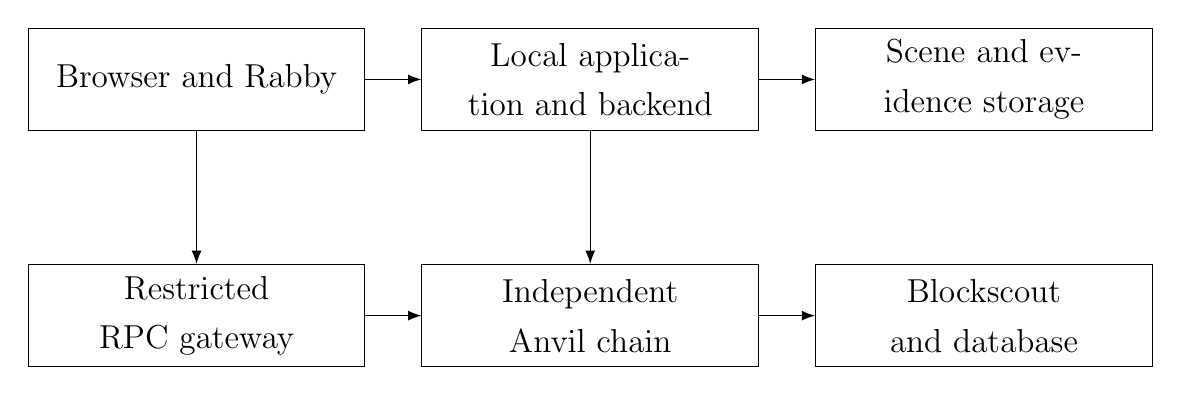
\begin{tikzpicture}[>=Latex,box/.style={draw,align=center,text width=4cm,minimum height=1.3cm}]
\node[box] (browser) at (0,0) {Browser and Rabby};
\node[box] (app) at (5,0) {Local application and backend};
\node[box] (data) at (10,0) {Scene and evidence storage};
\node[box] (rpc) at (0,-3) {Restricted RPC gateway};
\node[box] (chain) at (5,-3) {Independent Anvil chain};
\node[box] (explorer) at (10,-3) {Blockscout and database};
\draw[->] (browser)--(app);
\draw[->] (app)--(data);
\draw[->] (browser)--(rpc);
\draw[->] (rpc)--(chain);
\draw[->] (app)--(chain);
\draw[->] (chain)--(explorer);
\end{tikzpicture}\end{center}
\clearpage
\subsection{Installation, startup and health checks}
Prepare Node.js 22.19 or a newer 22.x release, npm, and running Docker with Compose. The scripts call docker-compose, so installations offering only docker compose need a compatible command first. Full deployment has primarily been validated on Apple Silicon Macs. Check image architecture on other platforms; the source-verification compiler uses amd64 and needs emulation on Apple Silicon. The first installation downloads npm dependencies, container images and explorer dependencies and therefore needs an internet connection.

Run these commands in a new directory. web3:init creates local configuration, web3:wallets exports this instance's test accounts, and web3:up builds and starts the application, node and explorer. Initial Blockscout migrations may take time. Wait for the health checks before connecting a wallet.

\begin{verbatim}
git clone https://github.com/Mengzhon001/deye-rwa-demo.git deye-rwa-local
cd deye-rwa-local
npm ci
DEYE_LOCAL_SOLC=1 npm run build
npm run web3:init
npm run web3:wallets
npm run web3:up
npm run web3:health
\end{verbatim}
Health checks cover the RPC Chain ID, application API, homepage, business page, documentation and Blockscout interface and API. If a check fails, use web3:status to inspect container status and web3:logs to inspect startup. Reinitializing wallets or deleting volumes is not a remedy for indexing delay. A healthy service does not itself prove source verification; inspect the relevant contract page in Blockscout.

\begin{verbatim}
npm run web3:status
npm run web3:logs
\end{verbatim}
\subsection{Local entry points and wallets}
Homepage\par\url{http://127.0.0.1:4174/}\par
Role sign-in and application\par\url{http://127.0.0.1:4174/app/}\par
Product documentation\par\url{http://127.0.0.1:4174/docs/}\par
Explorer\par\url{http://127.0.0.1:4000/}\par
Wallet RPC\par\url{http://127.0.0.1:18545}\par
Import the six accounts into Rabby from .data/local-wallets/wallet-import.private.json on your own machine. The file has mode 600 and the terminal prints addresses only. Verify Chain ID 20260922, choose the role and sign in. The generated accounts differ from the shared-environment addresses listed earlier in the manual; importing a shared role key does not automatically grant its role in a new instance.

\subsection{Empty scenes, data sources and workflow reproduction}
The public source excludes raw station records, API credentials and pre-issued products. An empty product hall on first startup is therefore expected. The intermediary opens Monitoring and evidence, explicitly selects Synthetic fixture as the source and confirms. The owner then submits an application for the sample station. The synthetic label must remain visible; the fixture tests workflow and does not prove a real asset's value.

Follow group B for application, quotation, review and signing, group C for credential approval, admission, valuation and publication, and group D for eligibility, subscription and settlement. Drafts do not appear in the investor hall. Group E covers actual household wallet payments, intermediary confirmation and distributions. Follow groups F to H for exits and expiry. Settlement still requires sufficient funds, and advancing time does not approve orders.

The standard local Docker profile exposes time controls under Demo tools: financial time at the bottom of the intermediary's Product operations page. Complete billing, payment, confirmation, expenses and valuation month by month before advancing, without relying on a maintenance-profile-specific guide shortcut. A bill does not mean cash has arrived; household payment and simulated grid-export funding still require separate reconciliation.

For real-data integration, obtain authorization and configure the station API on the server, or import validated recorded evidence. A container needs a read-only mount for the replay file, and DEYE\_REPLAY\_FILE must identify its container path rather than only a host filename. An API failure never silently selects synthetic data. Field mappings, units and suitability for valuation must still be checked; displaying numbers is not data certification.

\subsection{Development regression, shutdown and recovery}
After a code change, run the following checks from the repository root. They test types, contracts and guidance rules and do not replace real-wallet and browser acceptance. Perform the interface walkthrough in your own instance and retain hashes and business records.

\begin{verbatim}
npm run typecheck:ui
DEYE_LOCAL_SOLC=1 npm run test:onchain
npm run test:guidance
\end{verbatim}
For automated lifecycle regression, web3:e2e operates on your own local Docker instance. It backs up the scene, executes signed transactions, advances time and restores the scene, stopping services in the process. It is not a read-only check for the shared public environment. Use web3:down to stop and web3:up to restart; ordinary shutdown preserves volumes. Remove volumes only for an intentional complete rebuild after preserving the local wallets and deployment records.

\begin{verbatim}
npm run web3:e2e
npm run web3:down
npm run web3:up
npm run web3:health
\end{verbatim}
These commands follow the current repository scripts. This documentation revision does not restart or reset the existing public, Base Sepolia or maintenance environments, and successful document compilation is not a claim that a fresh machine has been deployed and tested. A new machine still needs its health checks and validation of wallets, container platform and data source.

\clearpage\section{Dynamic guidance and handoffs}
The first-entry introduction explains equipment, rights, money and participant responsibilities. The guide panel identifies the product, object, prerequisites, handler and expected result. Pause or collapse it and reopen Operation guide from the top bar. Completion comes from business and chain state rather than a Next button.

Participant mode focuses on the connected participant’s tasks and handoffs. Four-role demonstration mode can inspect other roles’ tasks and open their login entry. The correct wallet and a new signature are still required. It does not sign on behalf of another role or grant intermediary authority to an investor.

Locate operation opens the relevant page and identifies a control, field or prerequisite. If a condition is missing, use the specific remedy shown. Switch to the named reviewer, prepare the missing report or let the intermediary confirm the controlled time advancement. A read-only inspection is not presented as a blocked payment.

In the monthly cycle, a pending trustee approval must be completed first. The guide hands off to investors only after a new declaration creates an actual claimable amount. Fully paid earlier distributions do not remain the current task. Investors can distinguish historical payments, an undeclared current period and remaining NAV.

\clearpage
\subsection{Product overview and task entry}
\begin{center}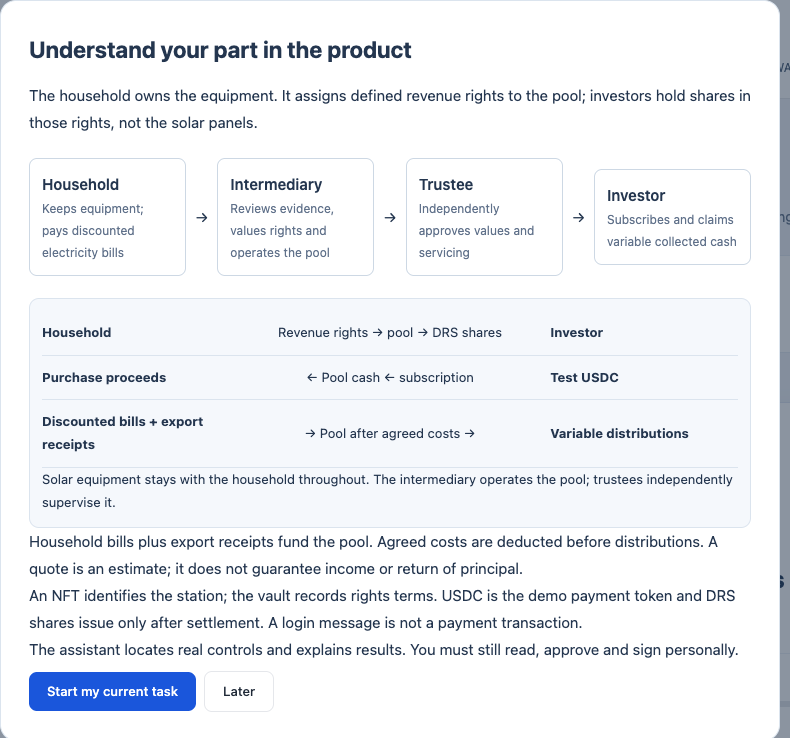
\includegraphics[width=\linewidth,height=.62\textheight,keepaspectratio]{assets/guide-overview.en.png}\par Read the overview and start the current task, or choose Later. The guide does not sign for a participant.\end{center}
\clearpage\begin{landscape}
\section{Application entry}
\subsection{A0 Application access}
\label{step:A0}
This step is performed by All participants. Open the public homepage and click Launch App. The browser should enter the current HTTPS application address and show the role selection dialog. If the environment is unavailable, ask the demonstration operator to check the Mac and tunnels.

After this step, select the intended role before connecting the wallet.

\begin{center}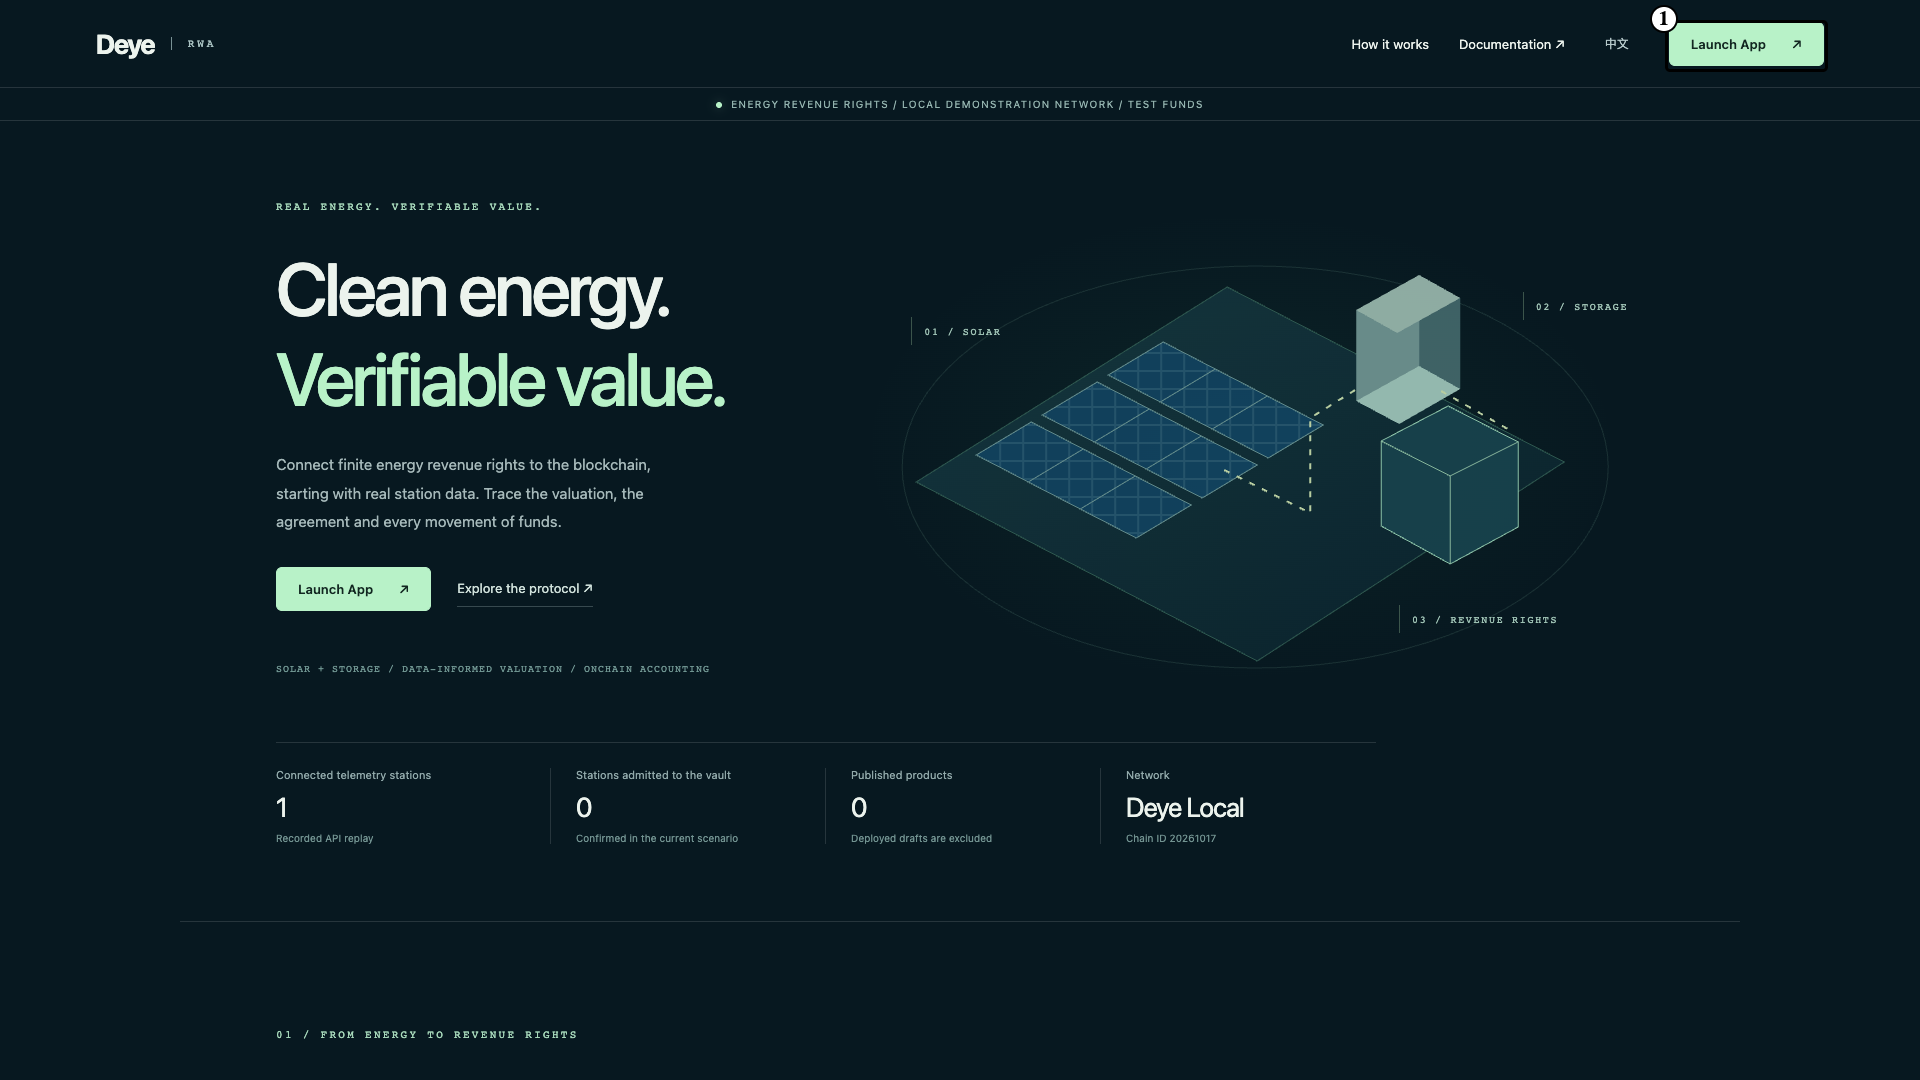
\includegraphics[width=\linewidth,height=.44\textheight,keepaspectratio]{assets/A0.en-context.png}\par Marker 1 identifies the control or information to inspect for this step. Amounts and dates refer to the isolated demonstration.\end{center}
\begin{center}
\includegraphics[width=.7\linewidth,height=1.55cm,keepaspectratio]{assets/A0.en-detail.png}\end{center}
\end{landscape}
\clearpage\begin{landscape}
\subsection{A1 Role selection and wallet sign-in}
\label{step:A1}
This step is performed by The participant performing the next task. Select the role, choose Rabby and click Connect wallet and sign in. In the extension, check the account, application domain, role and Chain ID before signing. A successful login opens the corresponding workspace without transferring funds.

After this step, continue in the selected role's workspace.

\begin{center}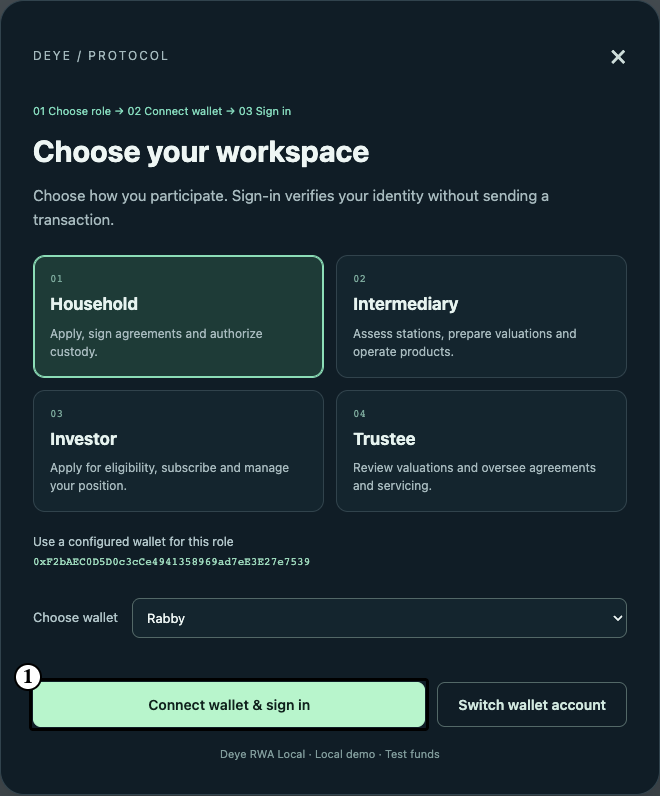
\includegraphics[width=\linewidth,height=.60\textheight,keepaspectratio]{assets/A1.en.png}\par Marker 1 identifies the control or information to inspect for this step. Amounts and dates refer to the isolated demonstration.\end{center}
\end{landscape}
\clearpage\begin{landscape}
\subsection{A2 Creation of an issuance draft}
\label{step:A2}
This step is performed by Intermediary. Click Create new series in the top bar. Enter the product name, acknowledge that this is a test and confirm deployment. The new draft has separate contracts and does not appear in the investor hall until fundraising is published.

After this step, ask the owner to select this same product before applying.

\begin{center}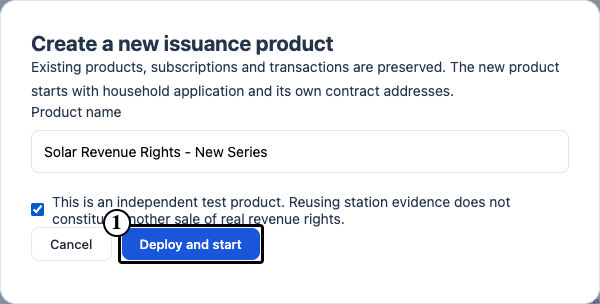
\includegraphics[width=\linewidth,height=.60\textheight,keepaspectratio]{assets/A2.en.png}\par Marker 1 identifies the control or information to inspect for this step. Amounts and dates refer to the isolated demonstration.\end{center}
\end{landscape}
\clearpage\begin{landscape}
\subsection{A3 Test funds for the selected product}
\label{step:A3}
This step is performed by The connected participant. Click Receive test funds in the top bar and check the wallet balances. The faucet supplies demo gas and the selected product's test USDC. It does not create an investment or issue DRS, and another product may have a different test USDC contract.

After this step, the investor can subscribe after qualification is approved.

\begin{center}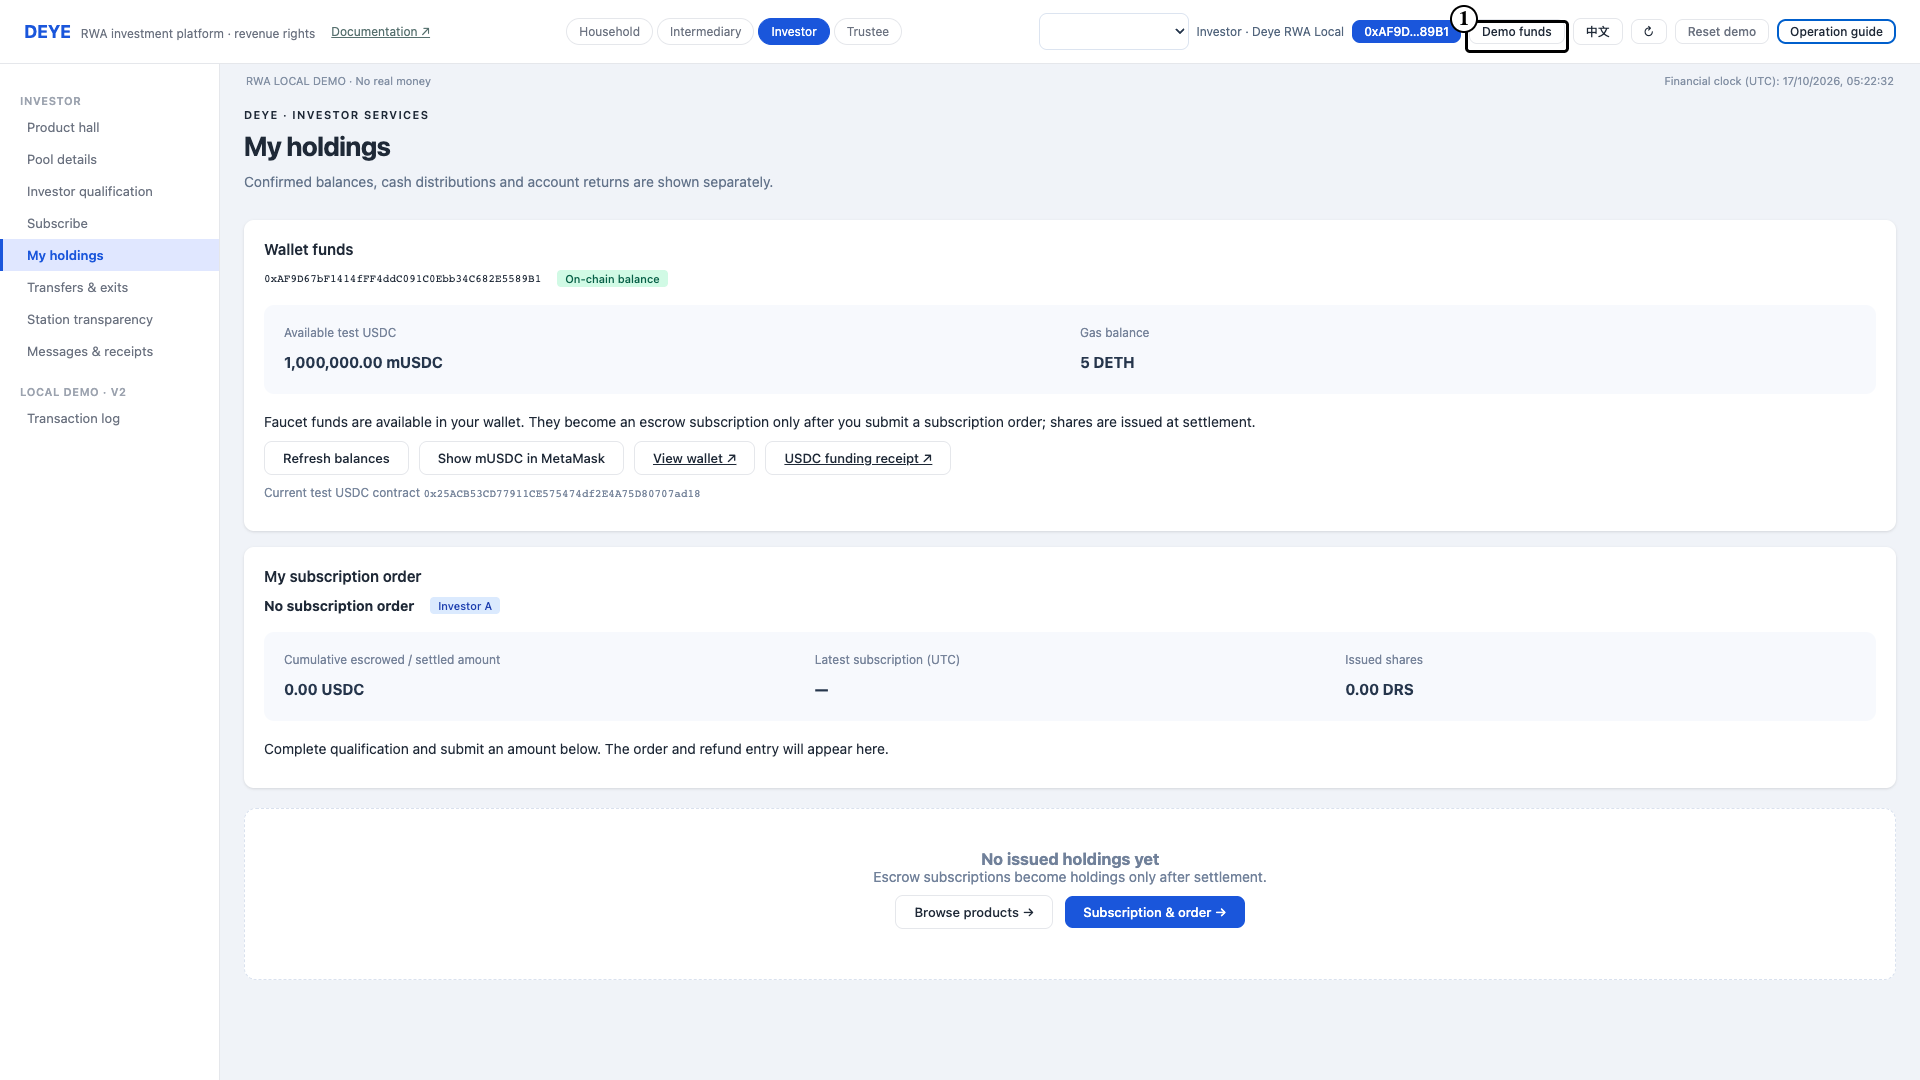
\includegraphics[width=\linewidth,height=.56\textheight,keepaspectratio]{assets/A3.en-context.png}\par Marker 1 identifies the control or information to inspect for this step. Amounts and dates refer to the isolated demonstration.\end{center}
\begin{center}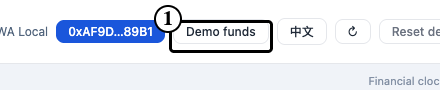
\includegraphics[width=.7\linewidth,height=1.55cm,keepaspectratio]{assets/A3.en-detail.png}\end{center}
\end{landscape}
\clearpage\begin{landscape}
\section{Application, valuation and agreement}
\subsection{B1 Station identity and evidence source}
\label{step:B1}
This step is performed by Owner. Open My stations and select the station details entry. Check the station identity, capacity and evidence timestamp before starting an application. The station list and the single-station dashboard serve different purposes.

After this step, review the detailed evidence and then submit an application.

\begin{center}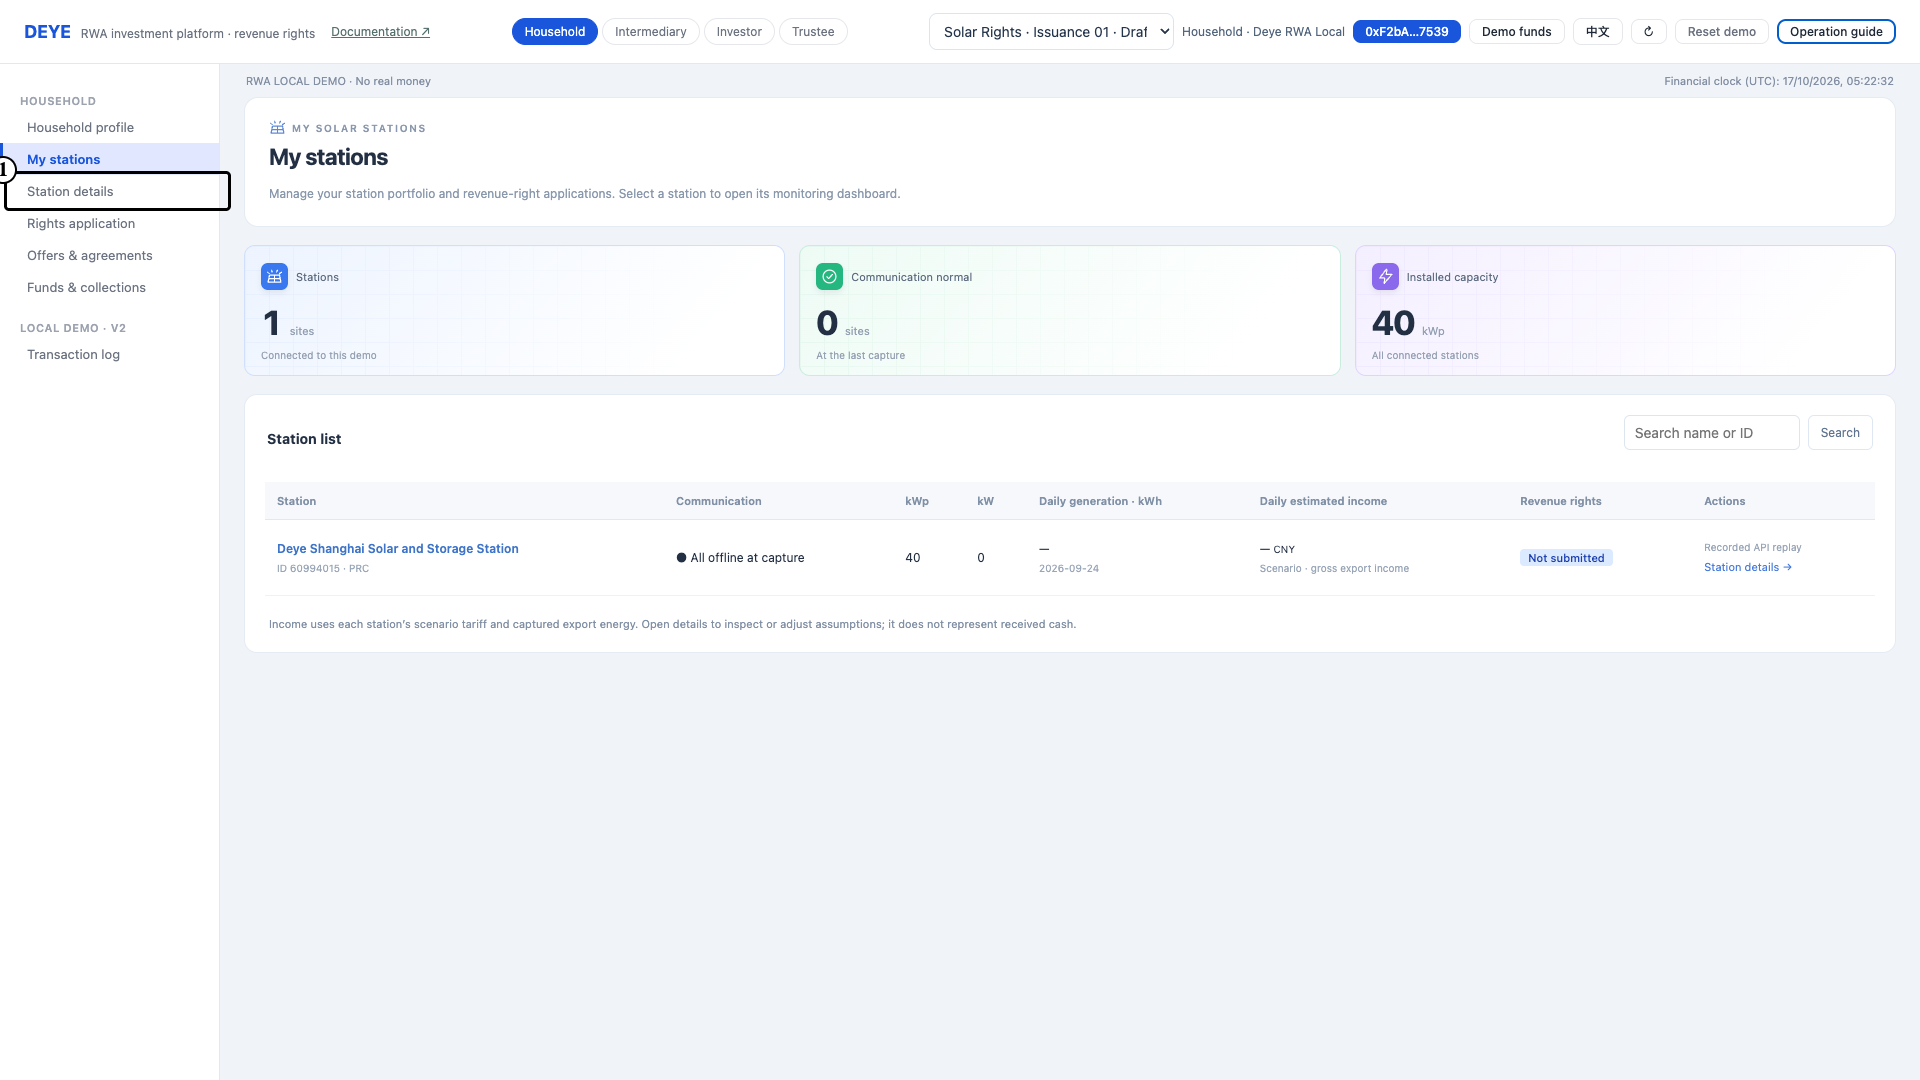
\includegraphics[width=\linewidth,height=.44\textheight,keepaspectratio]{assets/B1.en-context.png}\par Marker 1 identifies the control or information to inspect for this step. Amounts and dates refer to the isolated demonstration.\end{center}
\begin{center}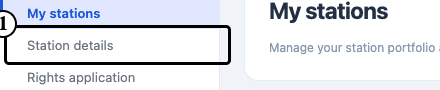
\includegraphics[width=.7\linewidth,height=1.55cm,keepaspectratio]{assets/B1.en-detail.png}\end{center}
\end{landscape}
\clearpage\begin{landscape}
\subsection{B2 Station dashboard review}
\label{step:B2}
This step is performed by Owner. Review generation, export, devices, alerts and the source badge in Station details. Recorded replay describes an earlier collection and is not a live reading. ALL\_OFFLINE is the reported telemetry status and does not by itself invalidate a blockchain product.

After this step, submit the revenue-right application for the selected station.

\begin{center}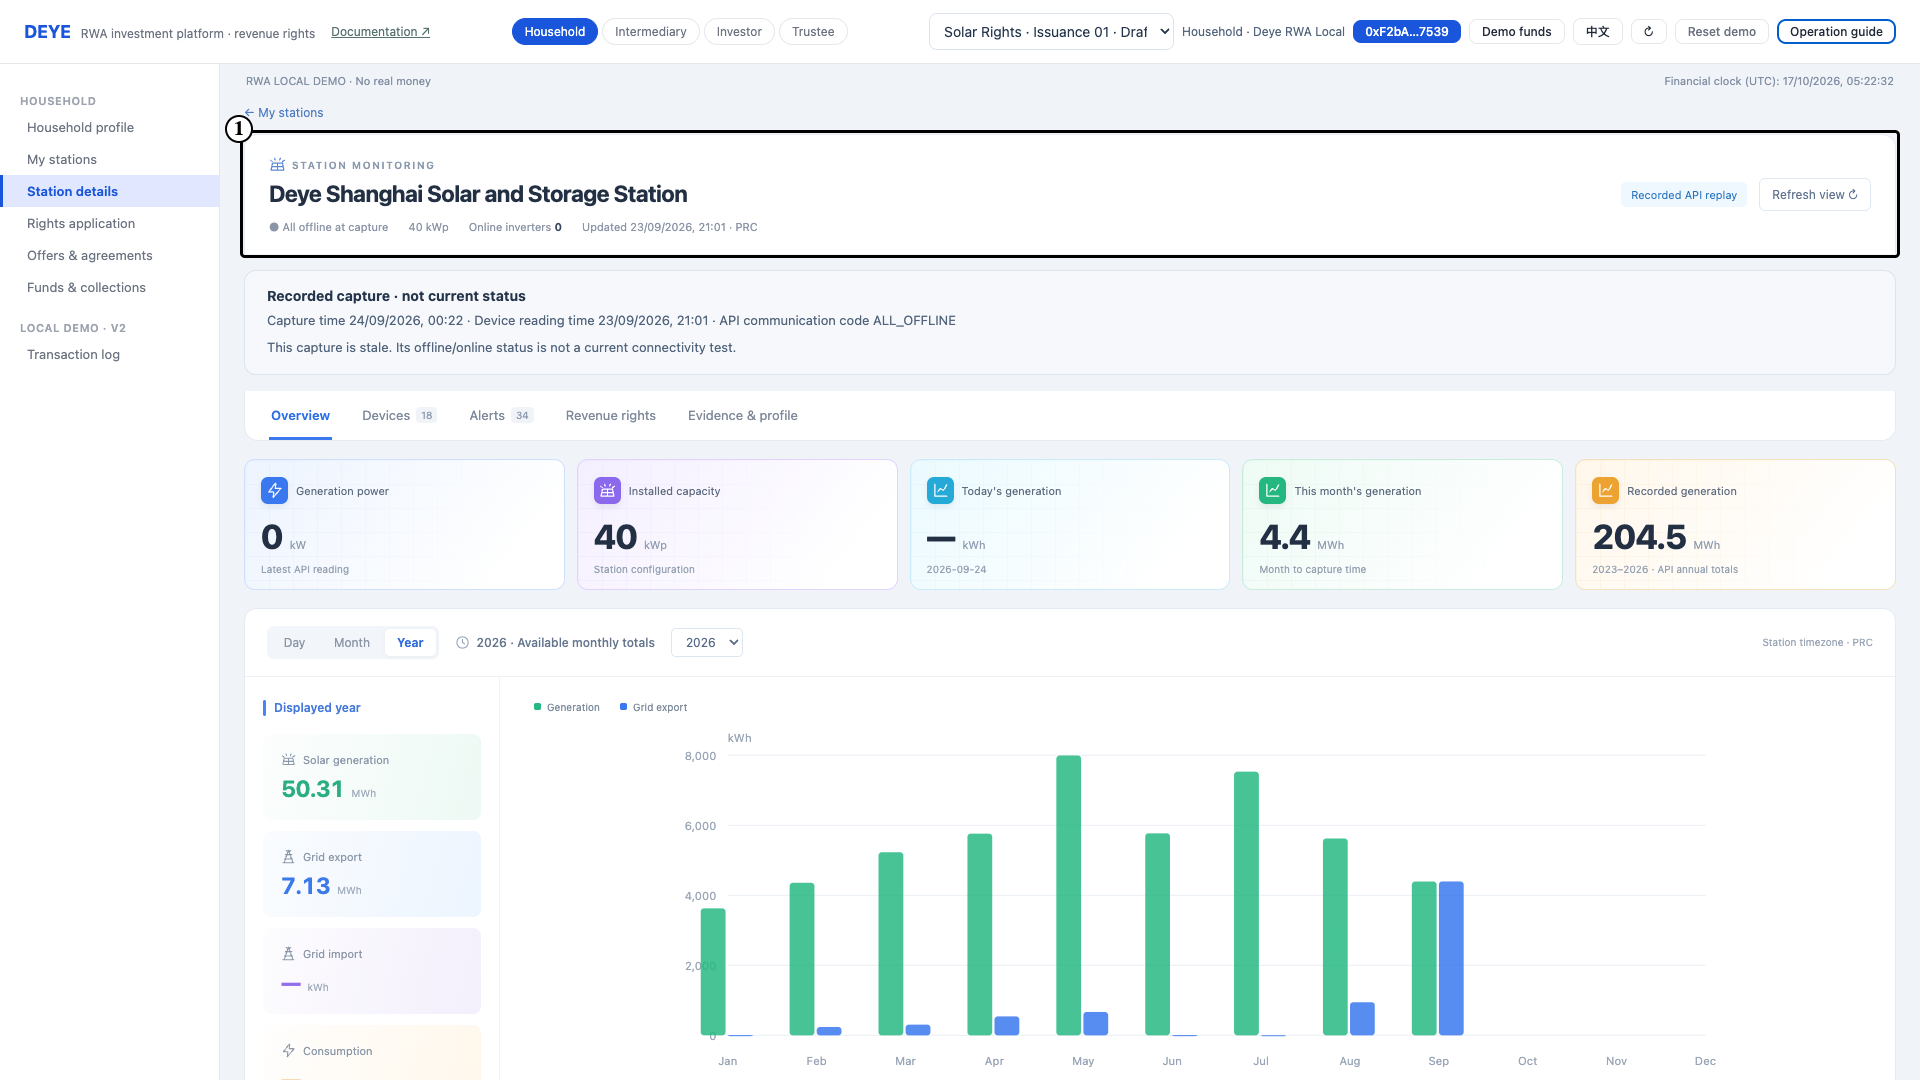
\includegraphics[width=\linewidth,height=.56\textheight,keepaspectratio]{assets/B2.en-context.png}\par Marker 1 identifies the control or information to inspect for this step. Amounts and dates refer to the isolated demonstration.\end{center}
\begin{center}
\includegraphics[width=.7\linewidth,height=1.55cm,keepaspectratio]{assets/B2.en-detail.png}\end{center}
\end{landscape}
\clearpage\begin{landscape}
\subsection{B3 Revenue-right application}
\label{step:B3}
This step is performed by Owner. Select the station and enter the requested information in the application form. Submit the record and retain its application identifier. This step stores the application and evidence references without minting an NFT or issuing investor shares.

After this step, the intermediary reviews the application queue.

\begin{center}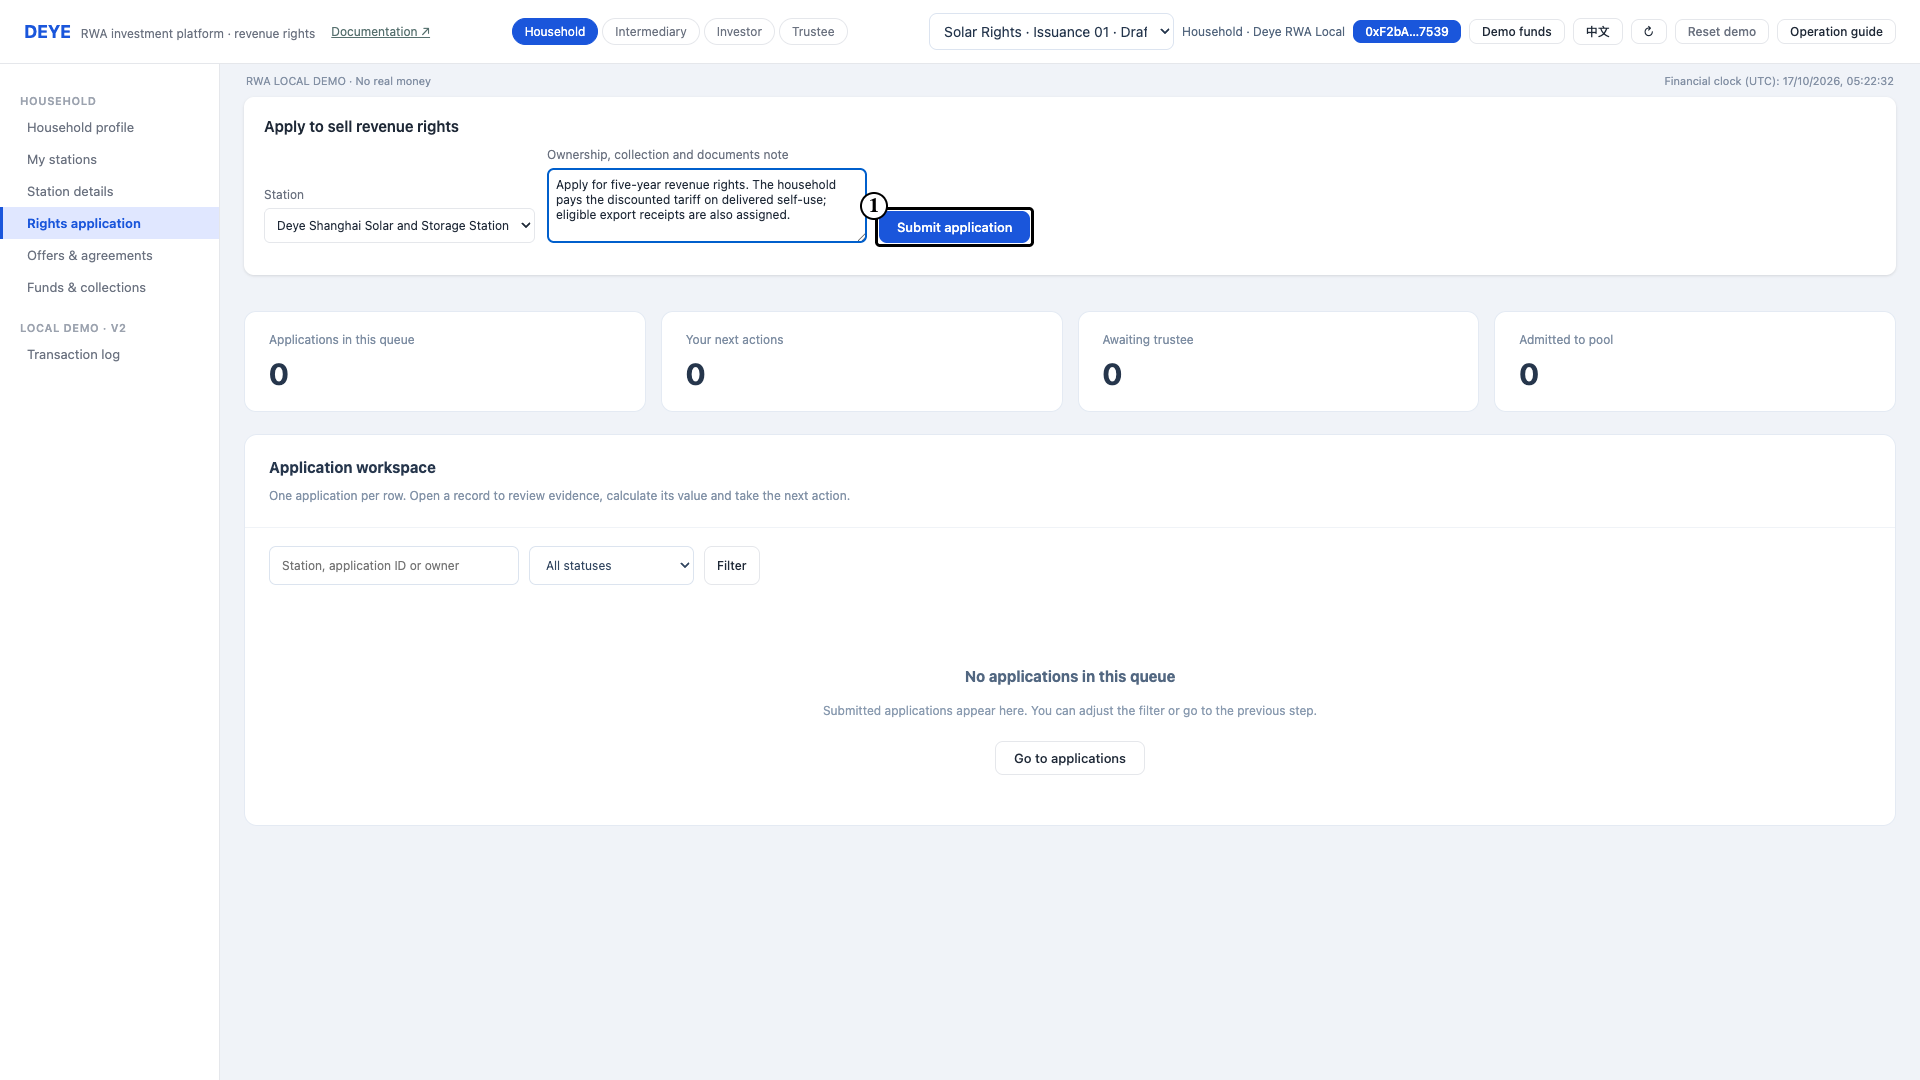
\includegraphics[width=\linewidth,height=.56\textheight,keepaspectratio]{assets/B3.en-context.png}\par Marker 1 identifies the control or information to inspect for this step. Amounts and dates refer to the isolated demonstration.\end{center}
\begin{center}
\includegraphics[width=.7\linewidth,height=1.55cm,keepaspectratio]{assets/B3.en-detail.png}\end{center}
\end{landscape}
\clearpage\begin{landscape}
\subsection{B4 Application queue}
\label{step:B4}
This step is performed by Intermediary. Open Application review and find the row for the relevant product and station. Check its status and next handler, then open the detailed record. Use the application identifier to distinguish separate requests for the same station.

After this step, review the evidence and terms in the application detail.

\begin{center}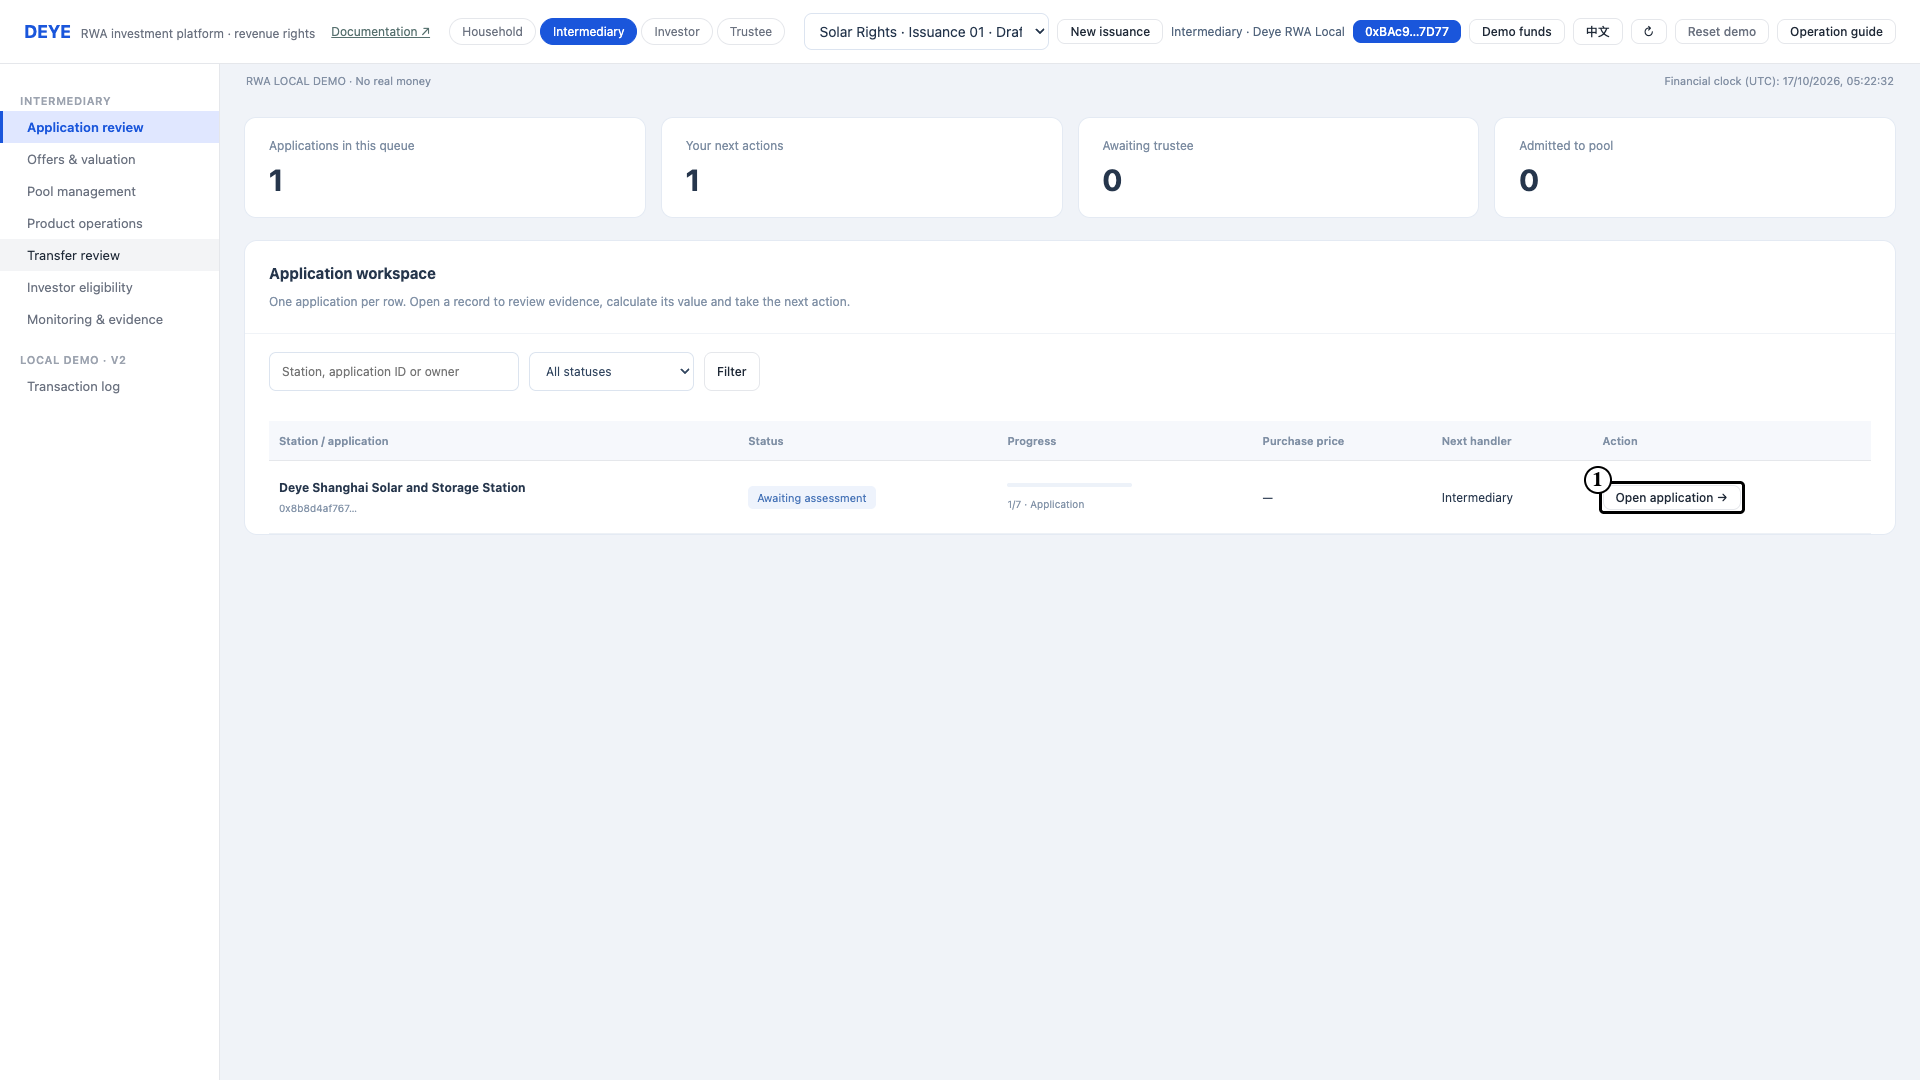
\includegraphics[width=\linewidth,height=.56\textheight,keepaspectratio]{assets/B4.en-context.png}\par Marker 1 identifies the control or information to inspect for this step. Amounts and dates refer to the isolated demonstration.\end{center}
\begin{center}
\includegraphics[width=.7\linewidth,height=1.55cm,keepaspectratio]{assets/B4.en-detail.png}\end{center}
\end{landscape}
\clearpage\begin{landscape}
\subsection{B5 Application assessment}
\label{step:B5}
This step is performed by Intermediary. Check station identity, evidence, the proposed rights scope and collection responsibilities. Approve complete materials or request supplementation with a clear explanation. A rejected or incomplete application must be resolved before pricing continues.

After this step, prepare the revenue-right offer for an approved application.

\begin{center}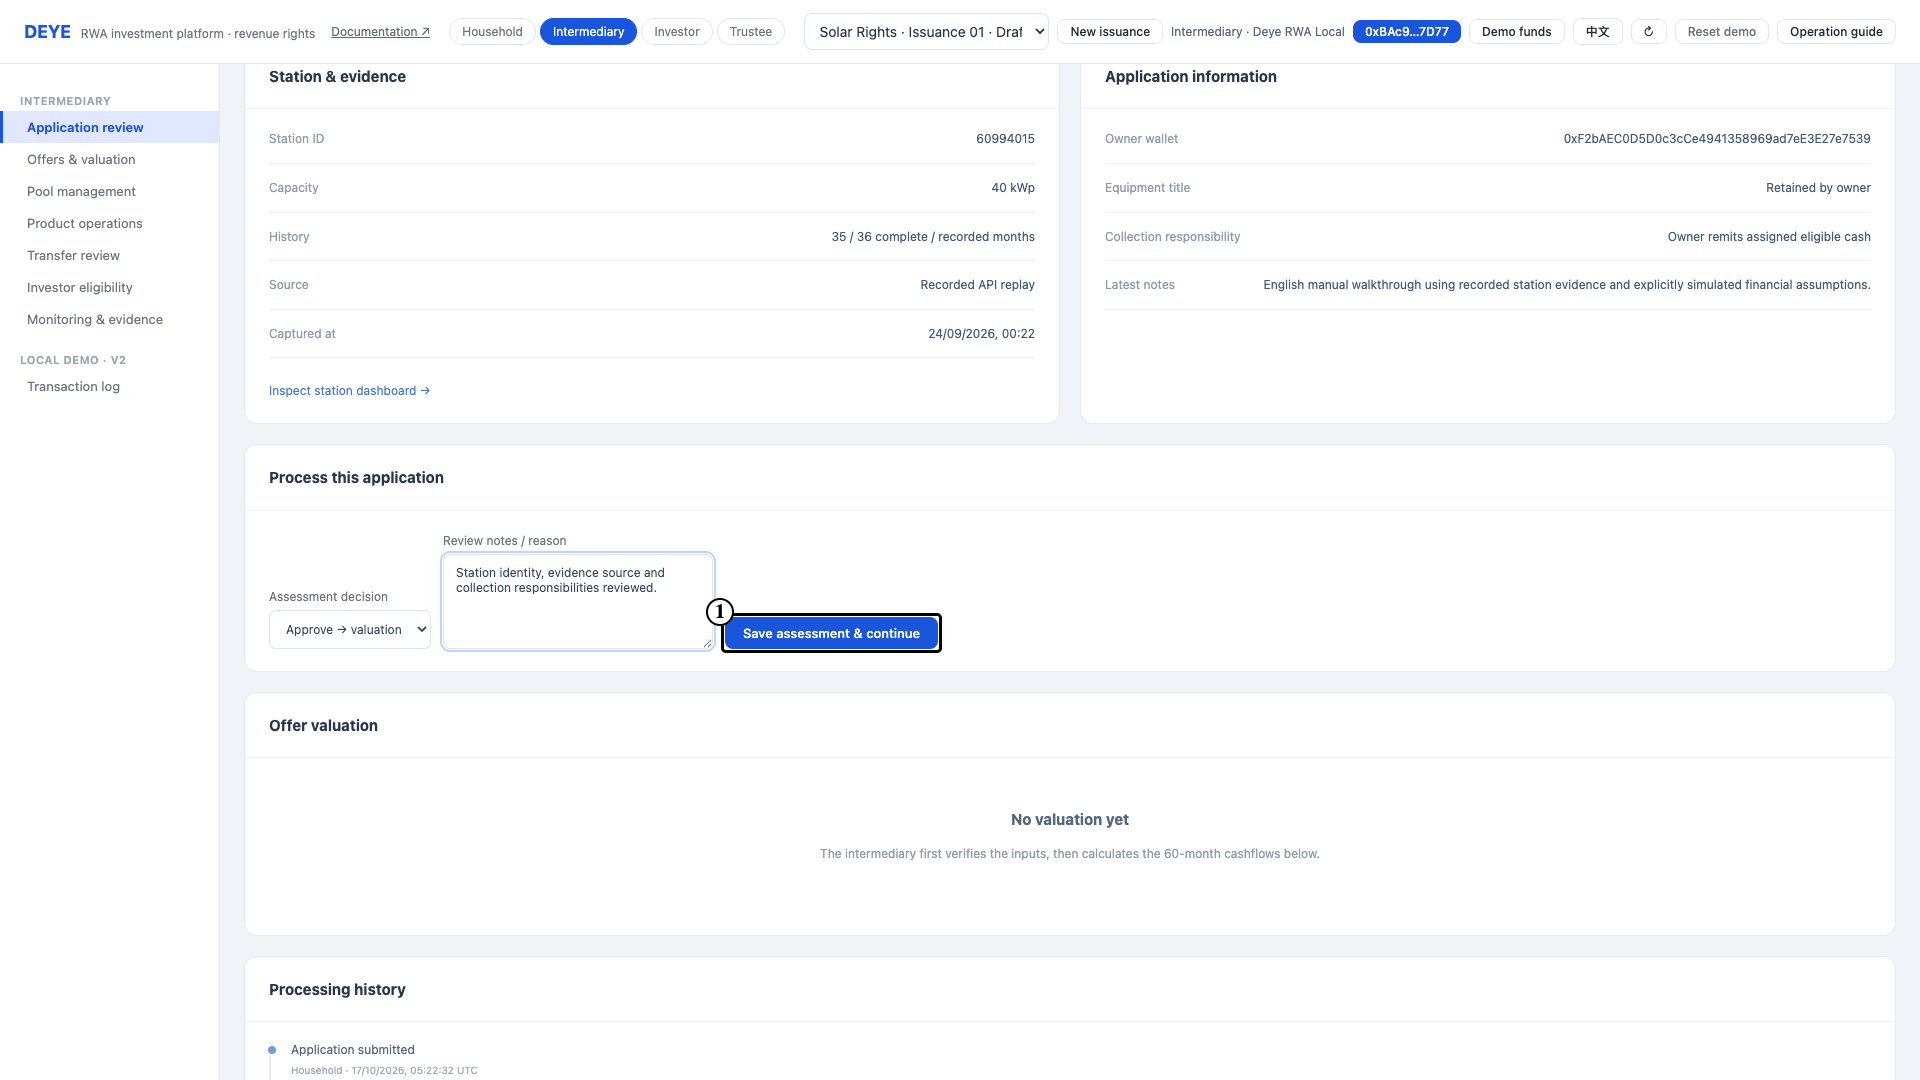
\includegraphics[width=\linewidth,height=.56\textheight,keepaspectratio]{assets/B5.en-context.png}\par Marker 1 identifies the control or information to inspect for this step. Amounts and dates refer to the isolated demonstration.\end{center}
\begin{center}
\includegraphics[width=.7\linewidth,height=1.55cm,keepaspectratio]{assets/B5.en-detail.png}\end{center}
\end{landscape}
\clearpage\begin{landscape}
\subsection{B6 Revenue-right valuation and offer}
\label{step:B6}
This step is performed by Intermediary. Open Quotes and valuation for the approved application. Review historical sample quality, seasonal generation and export estimates, delivered self-use, tariffs, owner discount, costs, FX and discounting. Record the reason for any provisional baseline before generating the offer.

After this step, the trustee independently reviews the offer and assumptions.

\begin{center}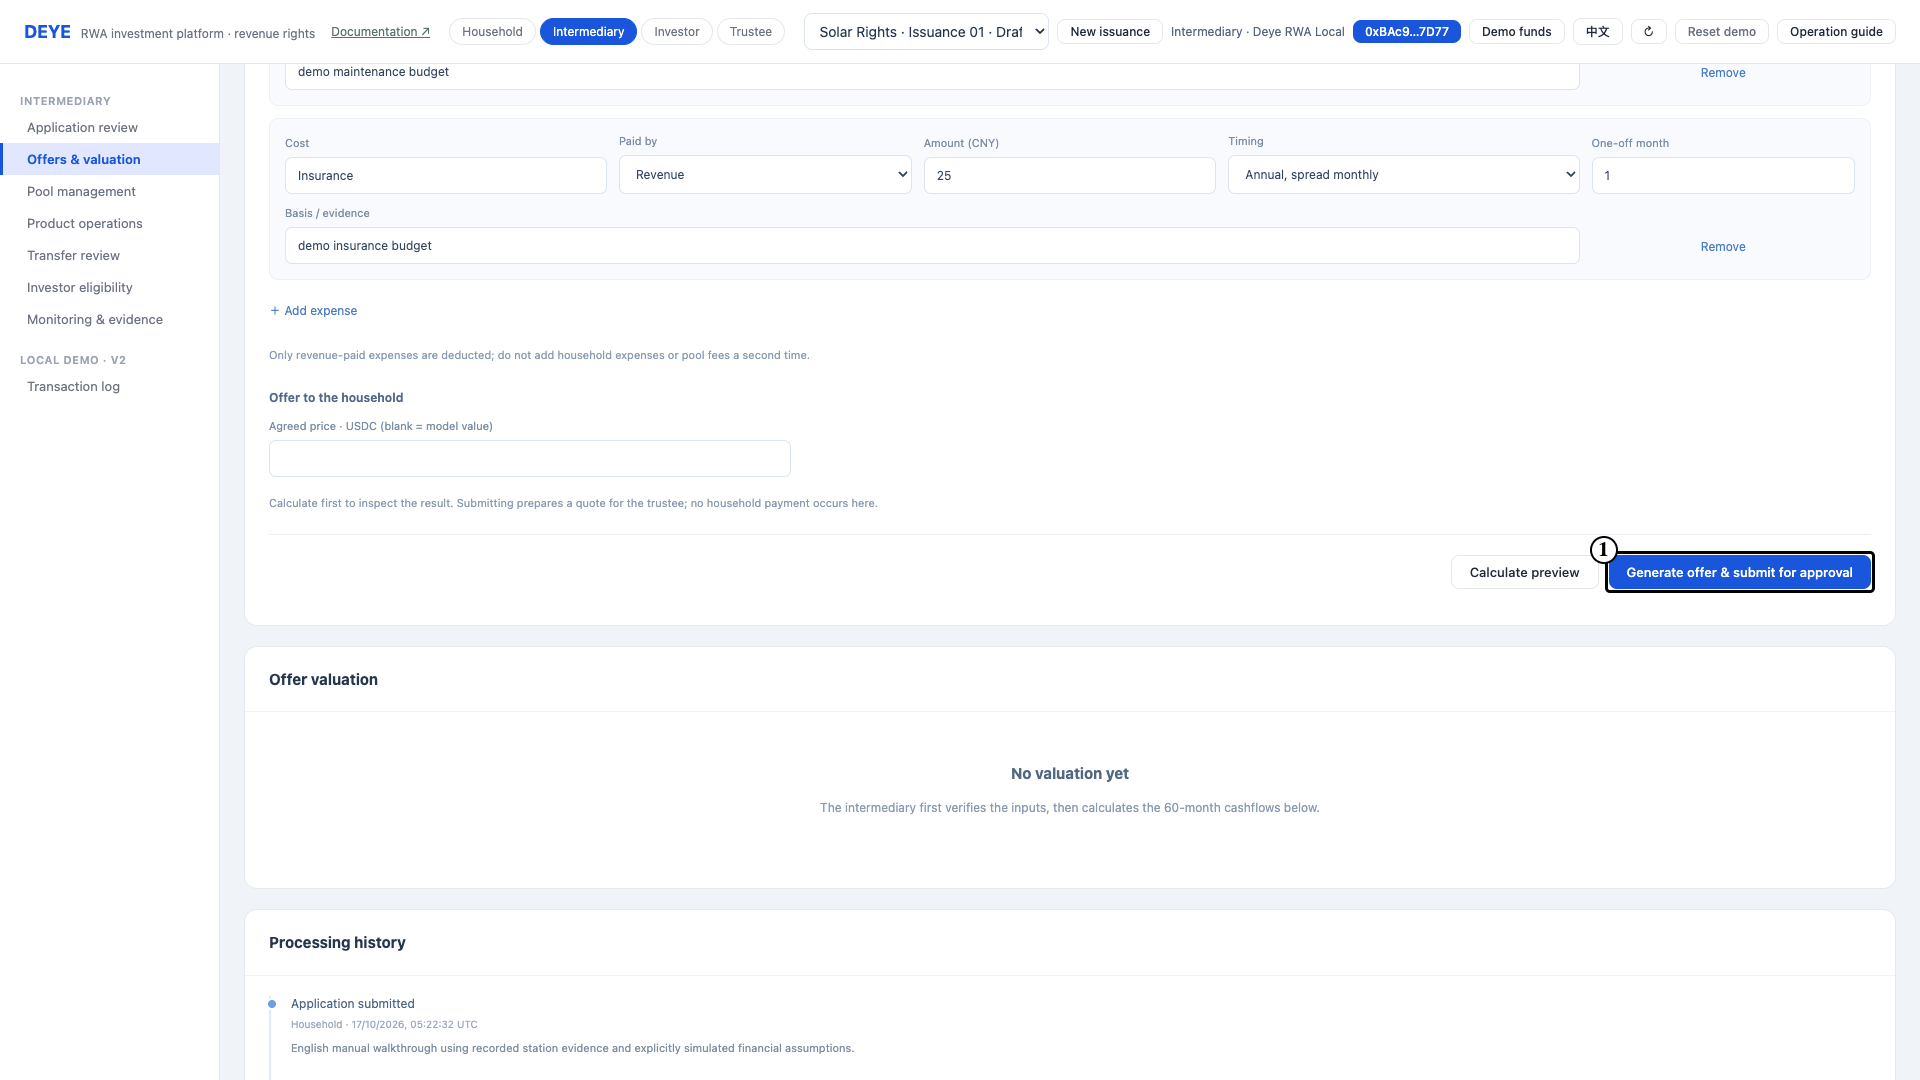
\includegraphics[width=\linewidth,height=.56\textheight,keepaspectratio]{assets/B6.en-context.png}\par Marker 1 identifies the control or information to inspect for this step. Amounts and dates refer to the isolated demonstration.\end{center}
\begin{center}
\includegraphics[width=.7\linewidth,height=1.55cm,keepaspectratio]{assets/B6.en-detail.png}\end{center}
\end{landscape}
\clearpage\begin{landscape}
\subsection{B7 Independent offer approval}
\label{step:B7}
This step is performed by Trustee. Open the application in the review queue and compare the forecast with its evidence and assumptions. Explicitly acknowledge provisional data when justified, then approve the offer. Approval does not sign the owner's agreement or transfer funds.

After this step, the owner reviews and accepts the approved offer.

\begin{center}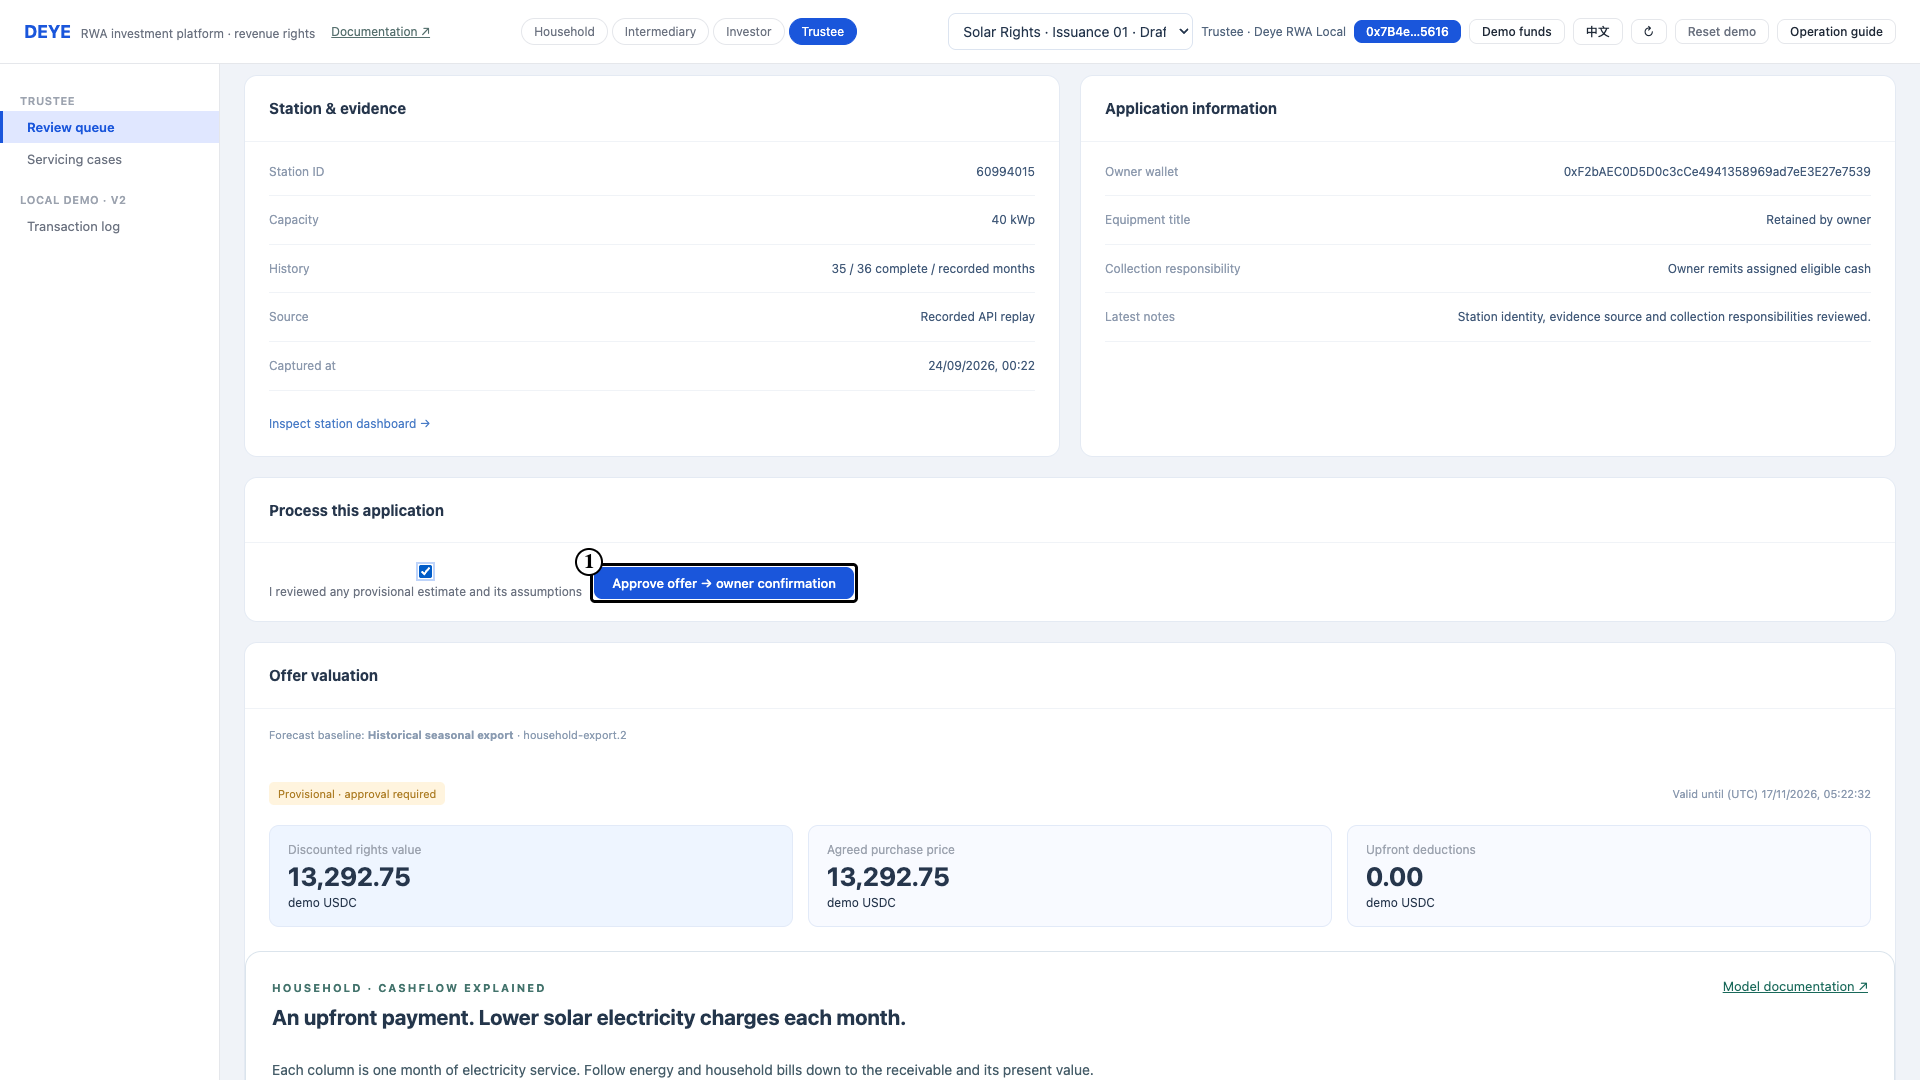
\includegraphics[width=\linewidth,height=.56\textheight,keepaspectratio]{assets/B7.en-context.png}\par Marker 1 identifies the control or information to inspect for this step. Amounts and dates refer to the isolated demonstration.\end{center}
\begin{center}
\includegraphics[width=.7\linewidth,height=1.55cm,keepaspectratio]{assets/B7.en-detail.png}\end{center}
\end{landscape}
\clearpage\begin{landscape}
\subsection{B8 Owner cashflow and electricity discount}
\label{step:B8}
This step is performed by Owner. Open the approved quote and inspect the monthly timeline from left to right. For each period, compare generation, export, delivered self-use, the grid-price comparison, the owner's discounted payment, export income, costs and discounted present value. These are forecasts rather than recorded receipts.

After this step, accept only after the price and future payment obligation are understood.

\begin{center}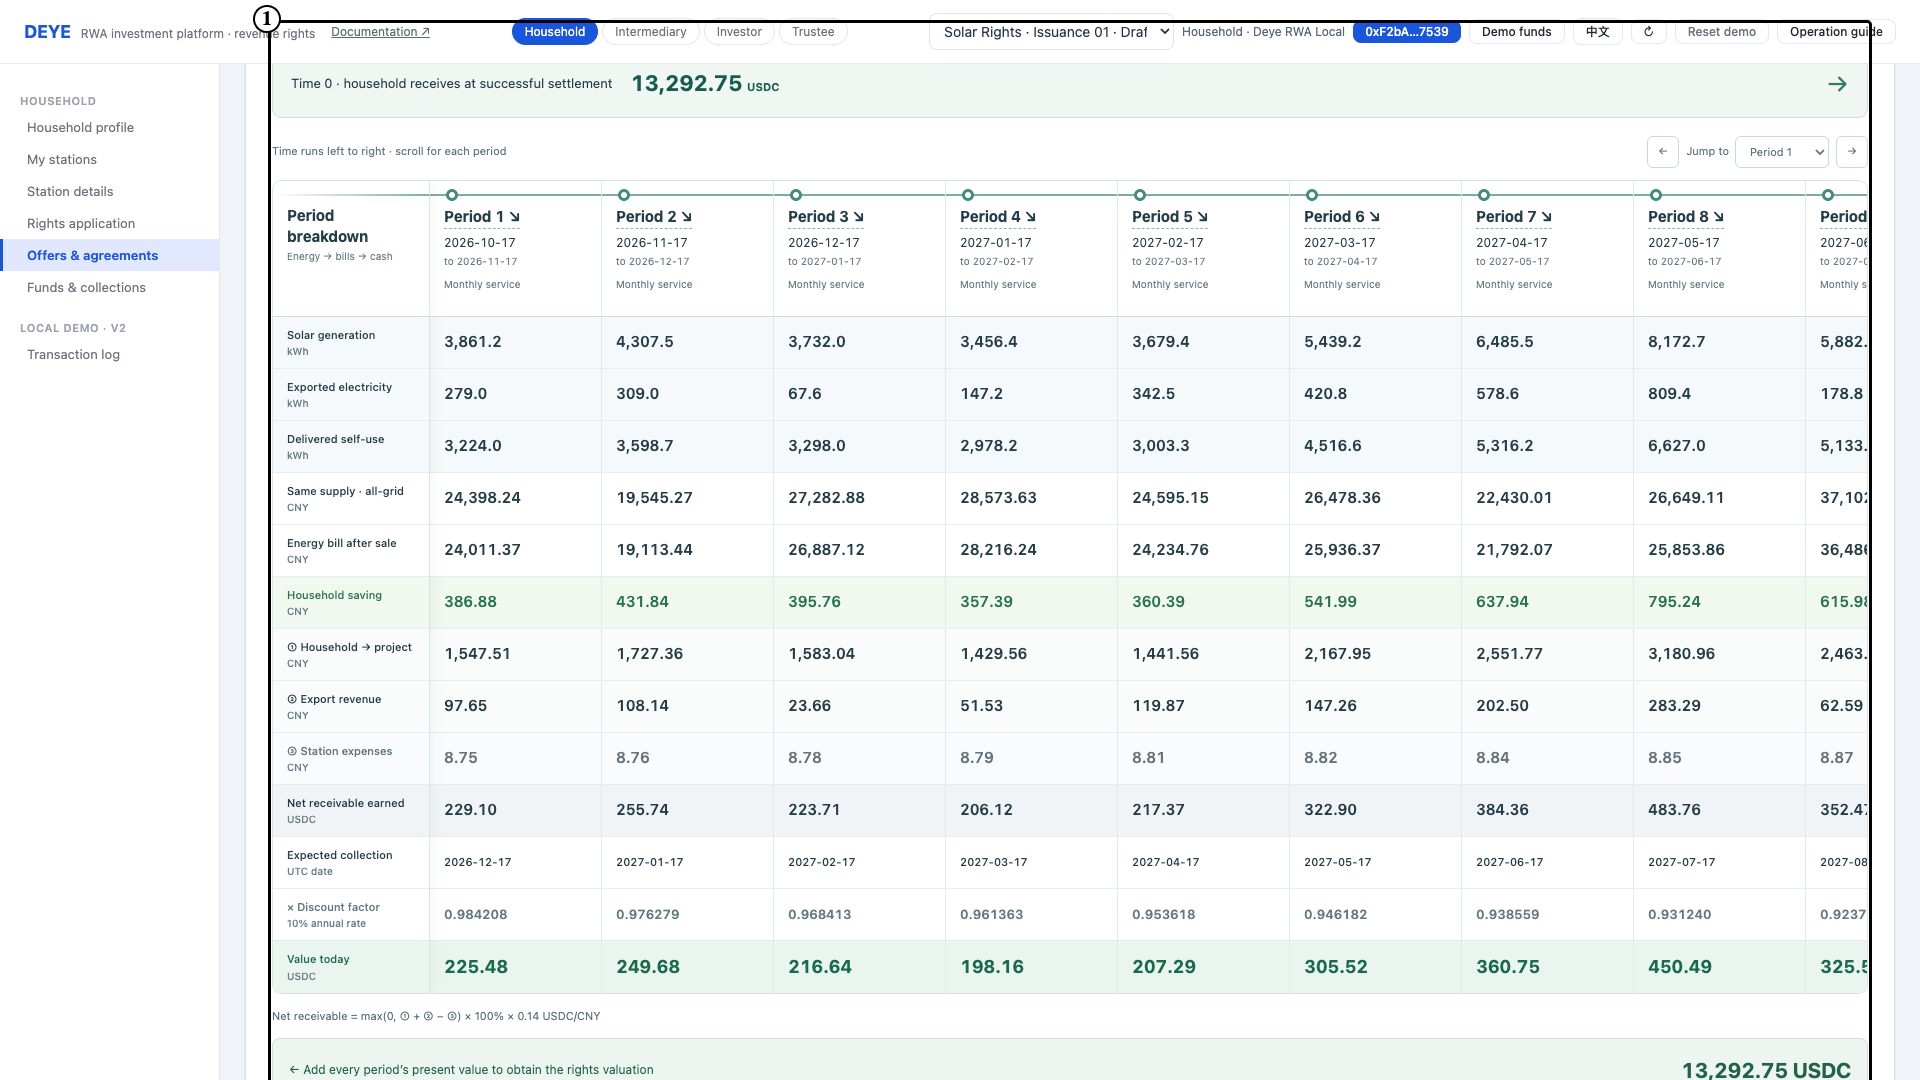
\includegraphics[width=\linewidth,height=.68\textheight,keepaspectratio]{assets/B8.en.png}\par Marker 1 identifies the control or information to inspect for this step. Amounts and dates refer to the isolated demonstration.\end{center}
\end{landscape}
\clearpage\begin{landscape}
\subsection{B9 Acceptance of the approved offer}
\label{step:B9}
This step is performed by Owner. Check the rights percentage, five-year term, purchase price, deductions and discounted electricity payment rule. Click Accept for the approved offer. Acceptance records consent to these terms and does not yet mint the station credential.

After this step, sign the corresponding agreement with the owner wallet.

\begin{center}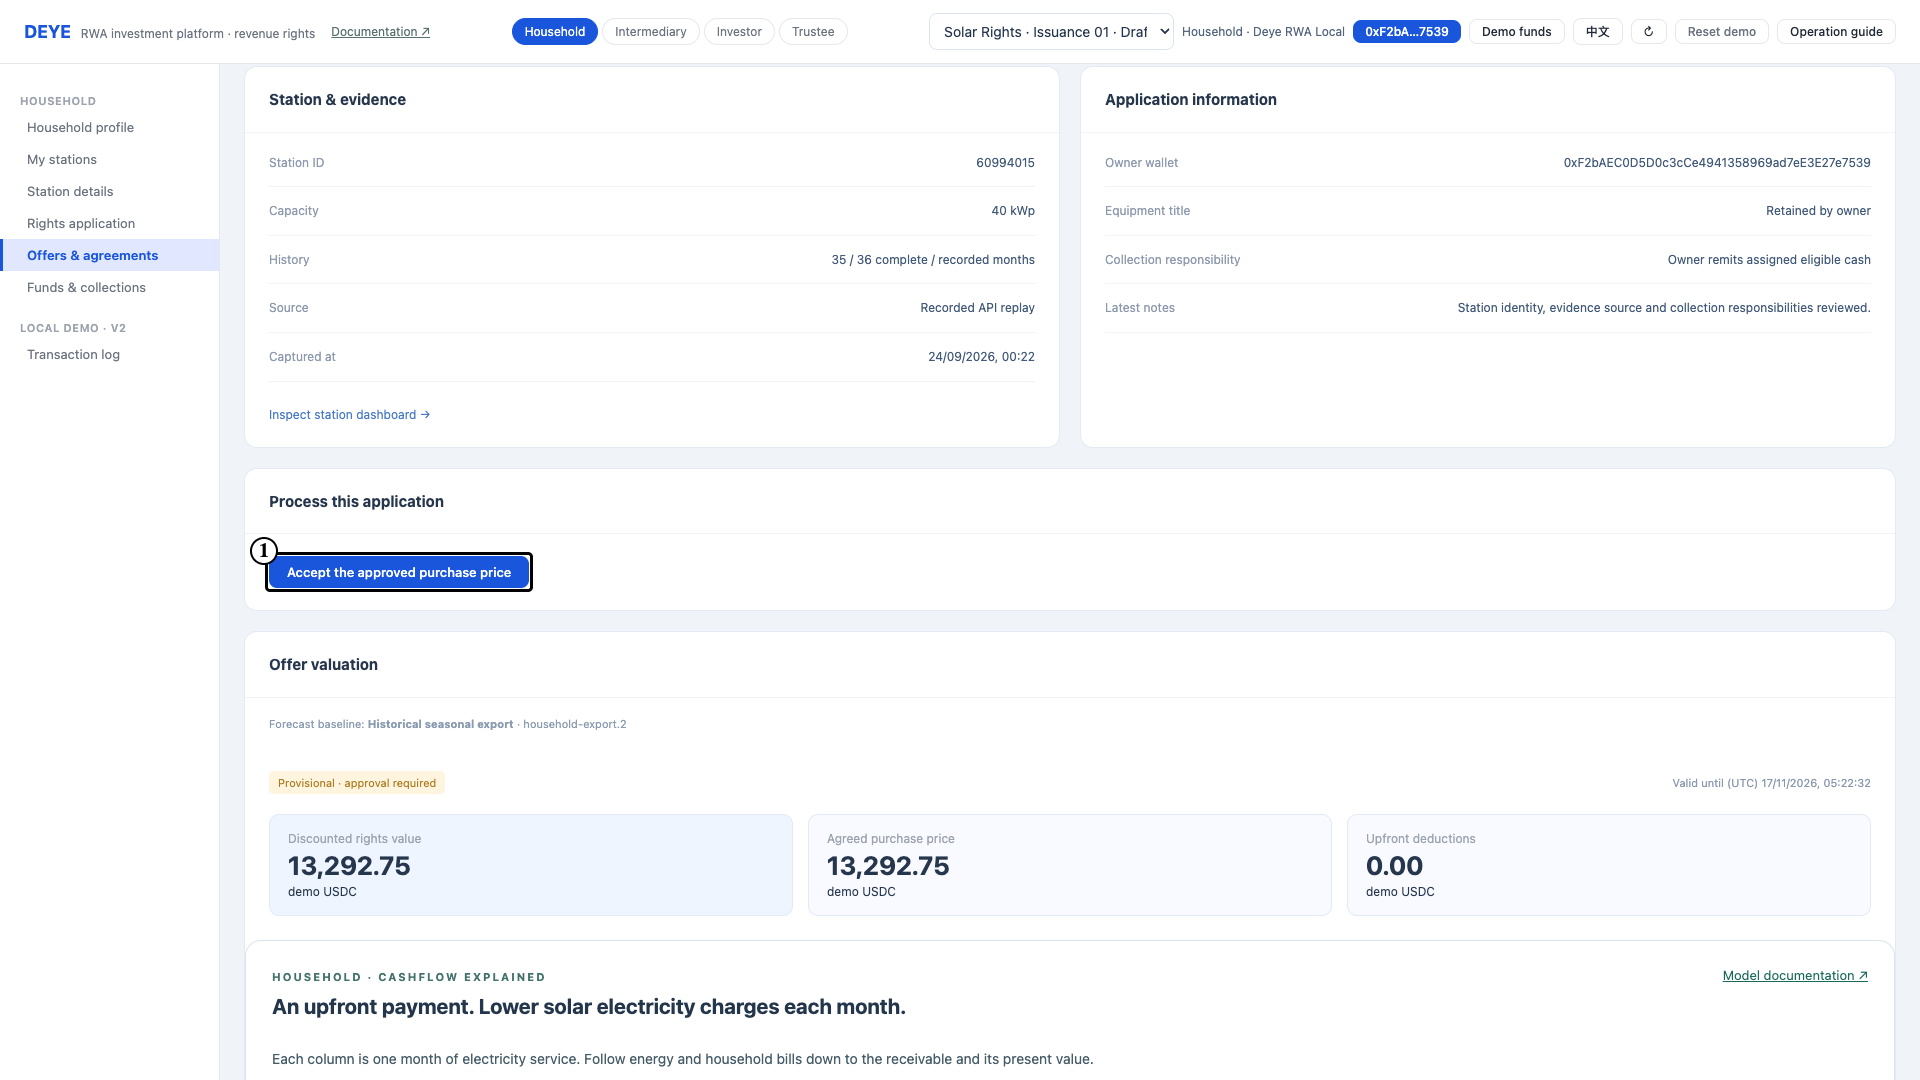
\includegraphics[width=\linewidth,height=.56\textheight,keepaspectratio]{assets/B9.en-context.png}\par Marker 1 identifies the control or information to inspect for this step. Amounts and dates refer to the isolated demonstration.\end{center}
\begin{center}
\includegraphics[width=.7\linewidth,height=1.55cm,keepaspectratio]{assets/B9.en-detail.png}\end{center}
\end{landscape}
\clearpage\begin{landscape}
\subsection{B10 Revenue-right agreement signature}
\label{step:B10}
This step is performed by Owner. Read the agreement and request the wallet signature. Verify the station, product, Chain ID, price, term and content digest in the message. The signature records agreement acceptance off-chain without transferring equipment ownership.

After this step, the intermediary mints the station identity credential.

\begin{center}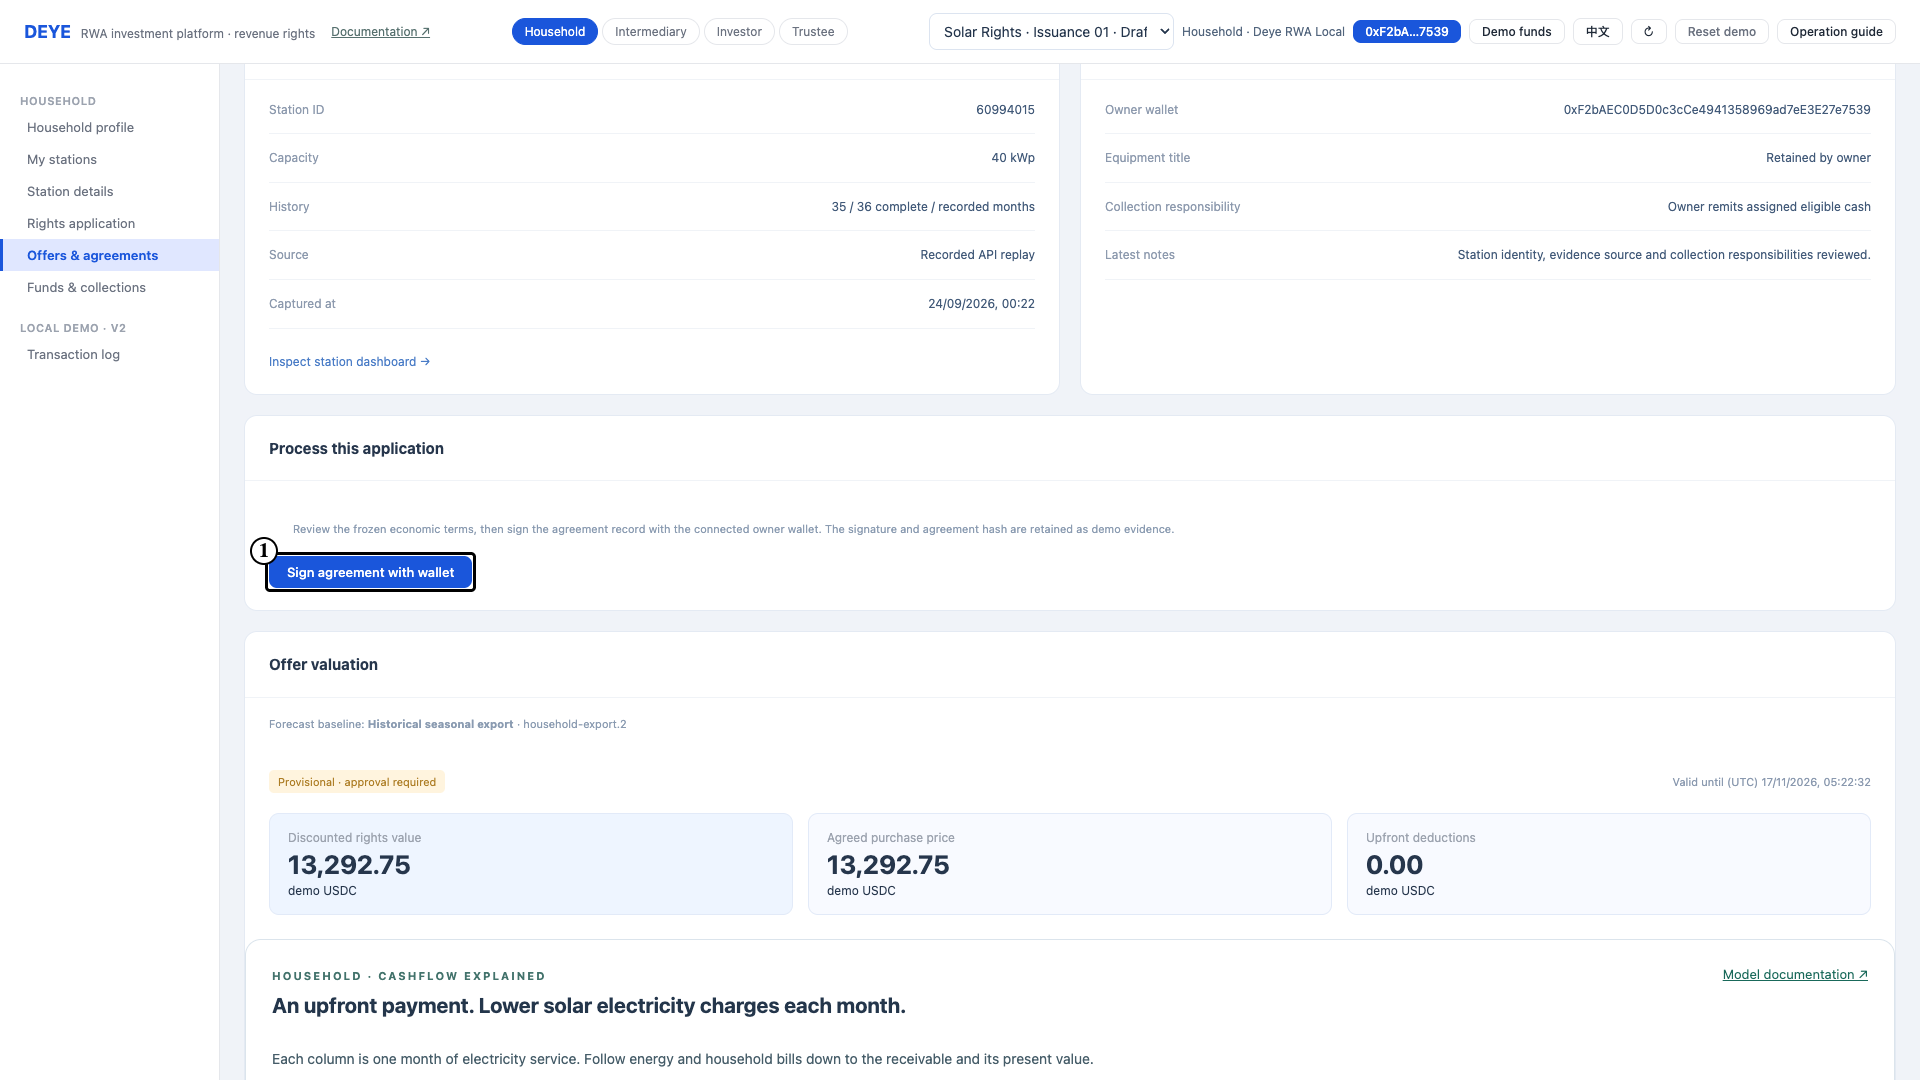
\includegraphics[width=\linewidth,height=.56\textheight,keepaspectratio]{assets/B10.en-context.png}\par Marker 1 identifies the control or information to inspect for this step. Amounts and dates refer to the isolated demonstration.\end{center}
\begin{center}
\includegraphics[width=.7\linewidth,height=1.55cm,keepaspectratio]{assets/B10.en-detail.png}\end{center}
\end{landscape}
\clearpage\begin{landscape}
\section{Credentials, admission and publication}
\subsection{C1 Station credential minting}
\label{step:C1}
This step is performed by Intermediary. In Pool management, open the signed application and click Mint station credential. Confirm the transaction with the intermediary wallet. After confirmation, the station NFT belongs to the owner and the transaction can be checked in Blockscout.

After this step, the owner authorizes custody by this pool.

\begin{center}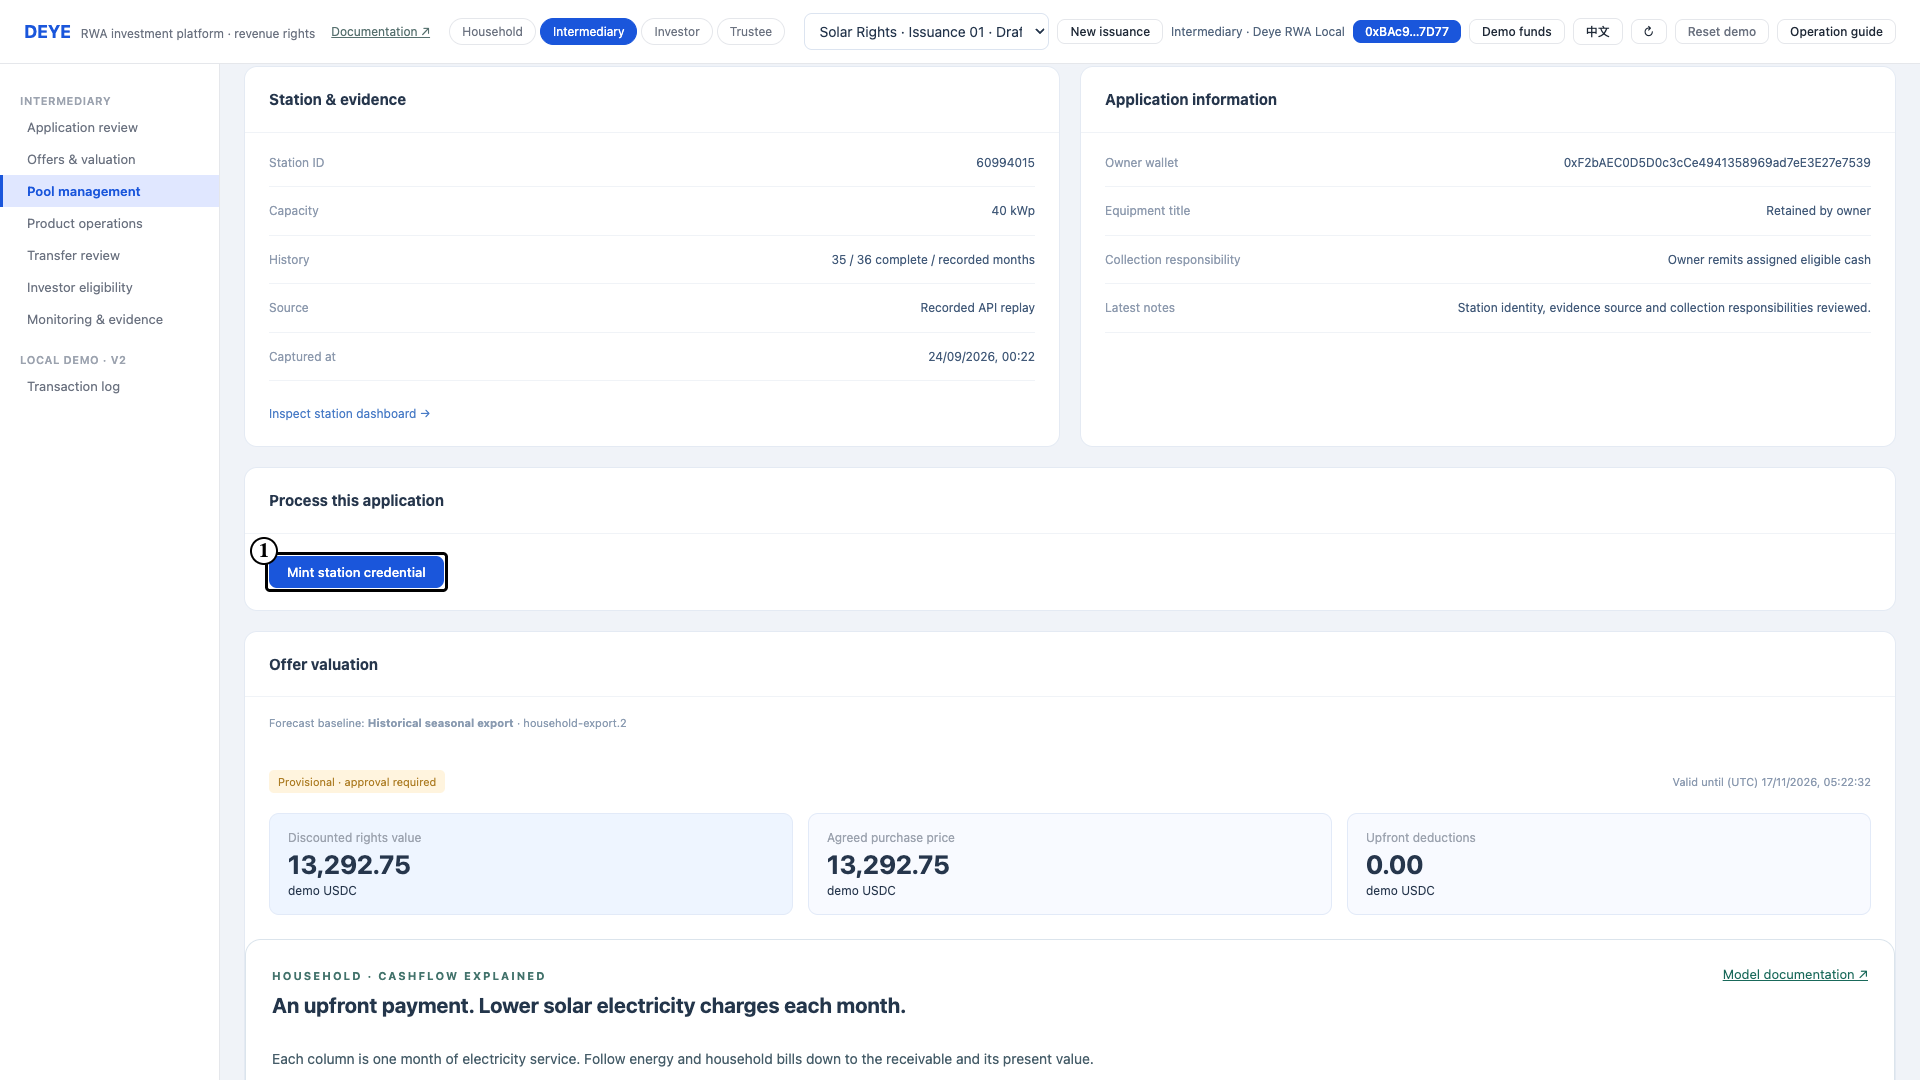
\includegraphics[width=\linewidth,height=.44\textheight,keepaspectratio]{assets/C1.en-context.png}\par Marker 1 identifies the control or information to inspect for this step. Amounts and dates refer to the isolated demonstration.\end{center}
\begin{center}
\includegraphics[width=.7\linewidth,height=1.55cm,keepaspectratio]{assets/C1.en-detail.png}\end{center}
\end{landscape}
\clearpage\begin{landscape}
\subsection{C2 Pool custody authorization}
\label{step:C2}
This step is performed by Owner. Open the agreement's custody task and check the station NFT and destination vault. Authorize this pool in the wallet and wait for chain confirmation. Approval permits custody but is not itself admission into the pool.

After this step, the intermediary executes admission after authorization is confirmed.

\begin{center}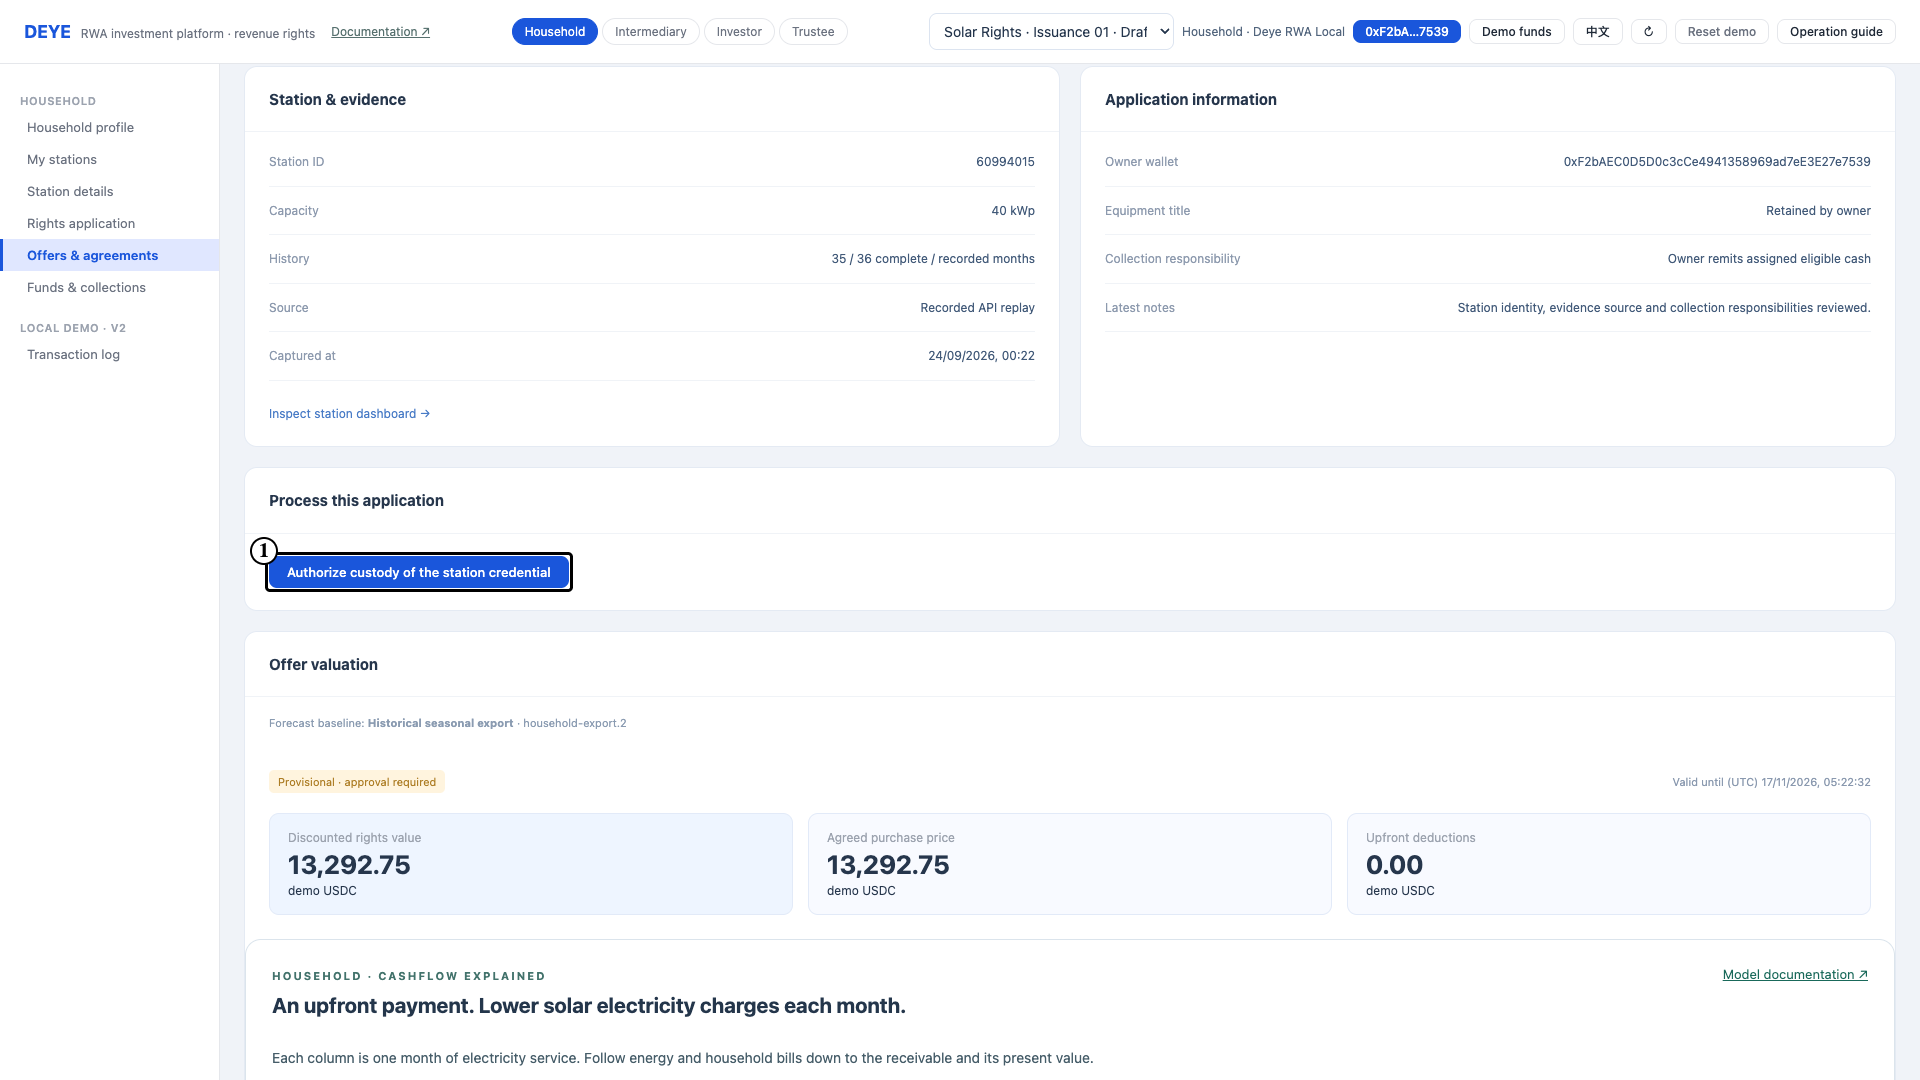
\includegraphics[width=\linewidth,height=.56\textheight,keepaspectratio]{assets/C2.en-context.png}\par Marker 1 identifies the control or information to inspect for this step. Amounts and dates refer to the isolated demonstration.\end{center}
\begin{center}
\includegraphics[width=.7\linewidth,height=1.55cm,keepaspectratio]{assets/C2.en-detail.png}\end{center}
\end{landscape}
\clearpage\begin{landscape}
\subsection{C3 Revenue-right admission}
\label{step:C3}
This step is performed by Intermediary. Check the signed agreement, owner authorization, purchase price and rights term, then execute admission. Confirm that the station NFT is held by the vault and the agreement digest is recorded. Admission does not mint investor shares.

After this step, prepare the pool valuation.

\begin{center}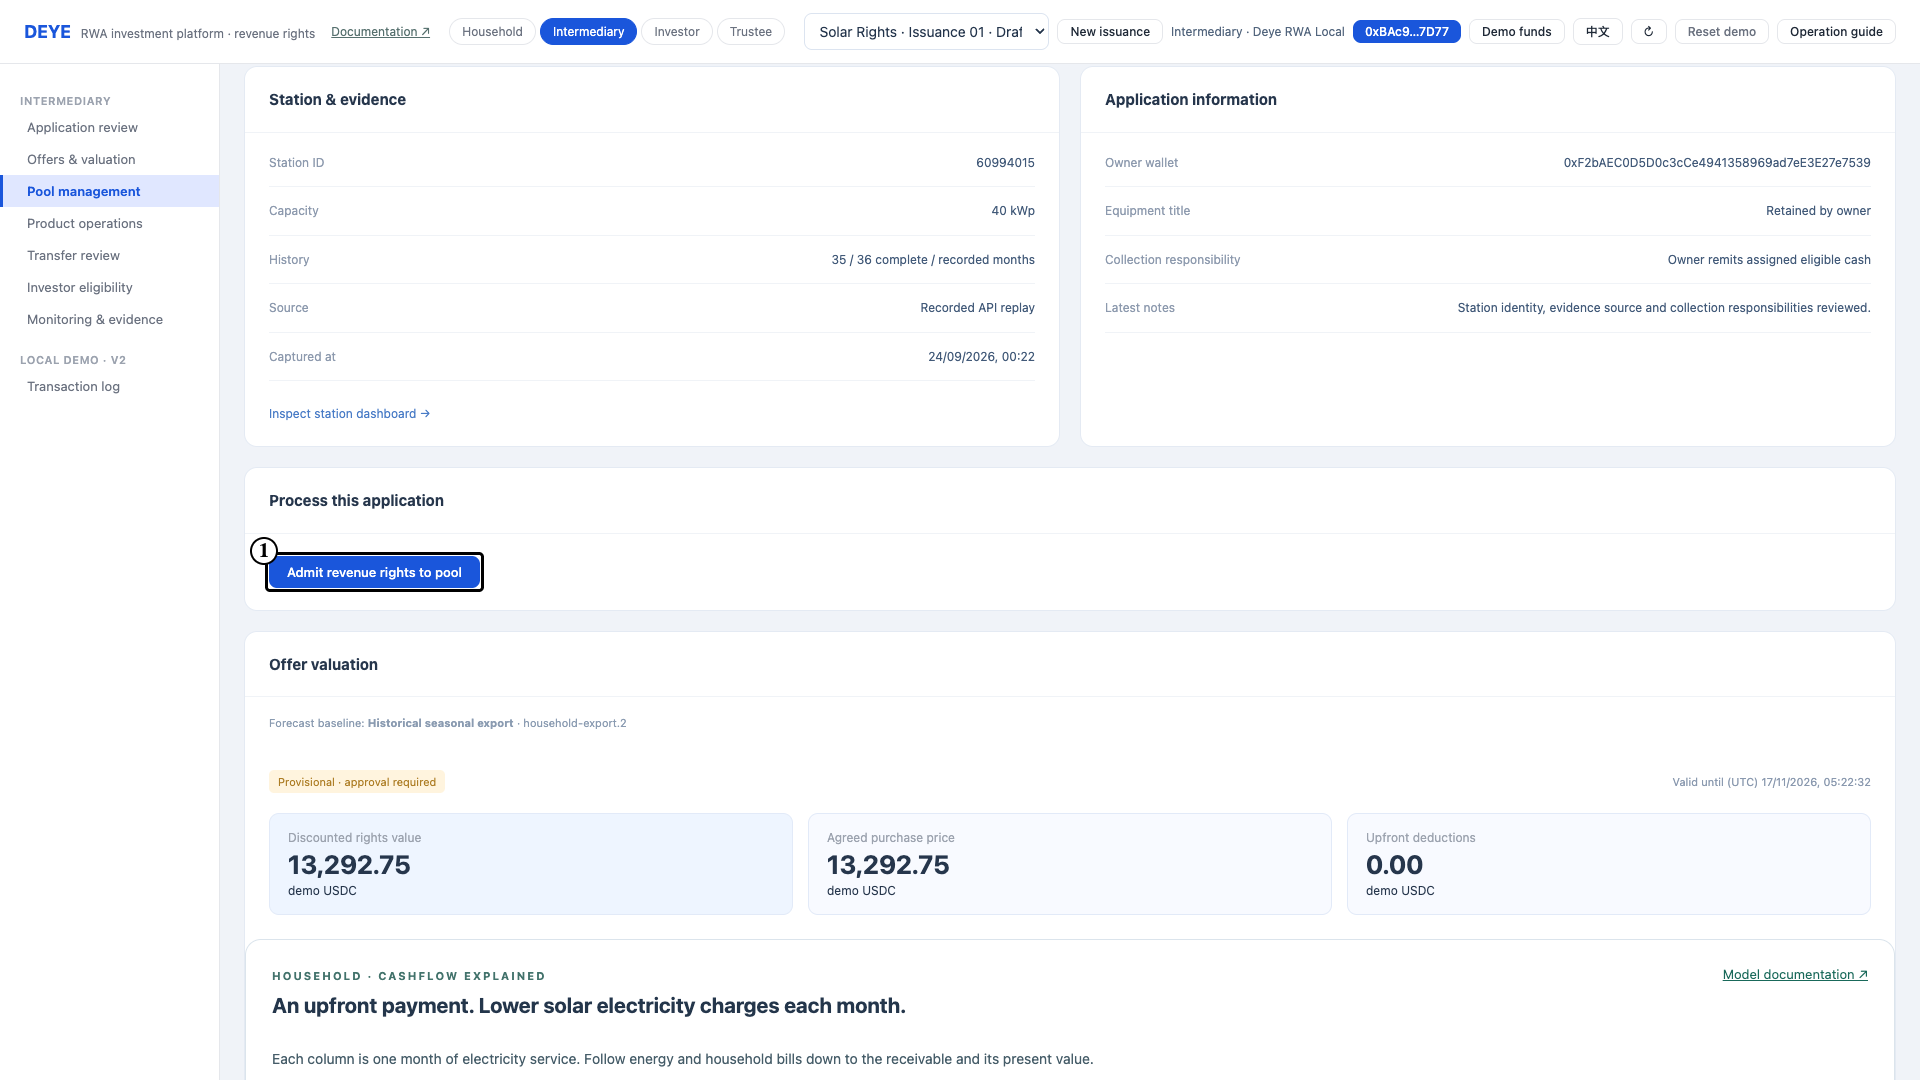
\includegraphics[width=\linewidth,height=.56\textheight,keepaspectratio]{assets/C3.en-context.png}\par Marker 1 identifies the control or information to inspect for this step. Amounts and dates refer to the isolated demonstration.\end{center}
\begin{center}
\includegraphics[width=.7\linewidth,height=1.55cm,keepaspectratio]{assets/C3.en-detail.png}\end{center}
\end{landscape}
\clearpage\begin{landscape}
\subsection{C4 Pool valuation submission}
\label{step:C4}
This step is performed by Intermediary. Prepare the pool report after reconciling rights value, cash, receivables, liabilities and future pool expenses. Confirm the submission transaction and retain its report digest and validity period. A material cashflow change may require a new report.

After this step, the trustee approves the submitted report.

\begin{center}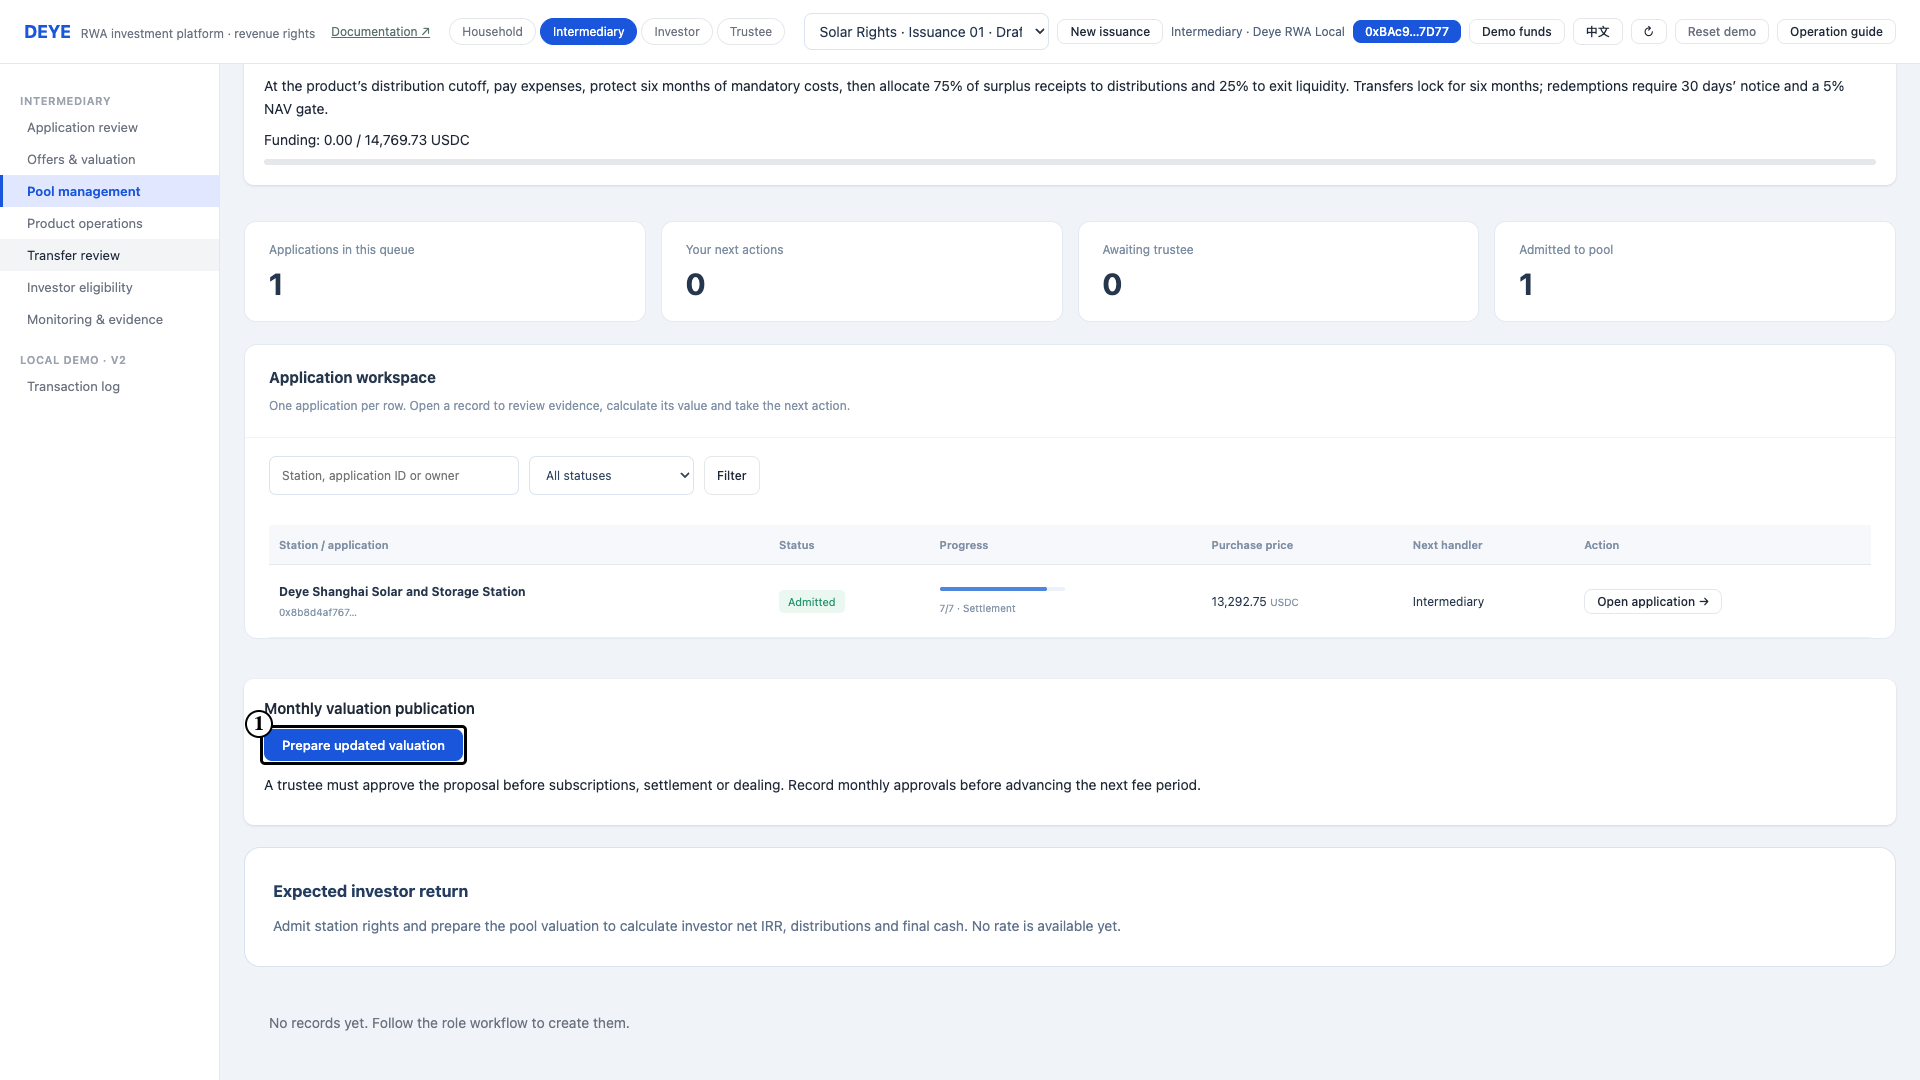
\includegraphics[width=\linewidth,height=.56\textheight,keepaspectratio]{assets/C4.en-context.png}\par Marker 1 identifies the control or information to inspect for this step. Amounts and dates refer to the isolated demonstration.\end{center}
\begin{center}
\includegraphics[width=.7\linewidth,height=1.55cm,keepaspectratio]{assets/C4.en-detail.png}\end{center}
\end{landscape}
\clearpage\begin{landscape}
\subsection{C5 Pool valuation approval}
\label{step:C5}
This step is performed by Trustee. Review the current report and explicitly check the assumptions acknowledgement before clicking Approve and anchor valuation. Confirm with the trustee wallet. An expired or changed report must return to the intermediary for preparation rather than being forced through approval.

After this step, the intermediary publishes fundraising after approval.

\begin{center}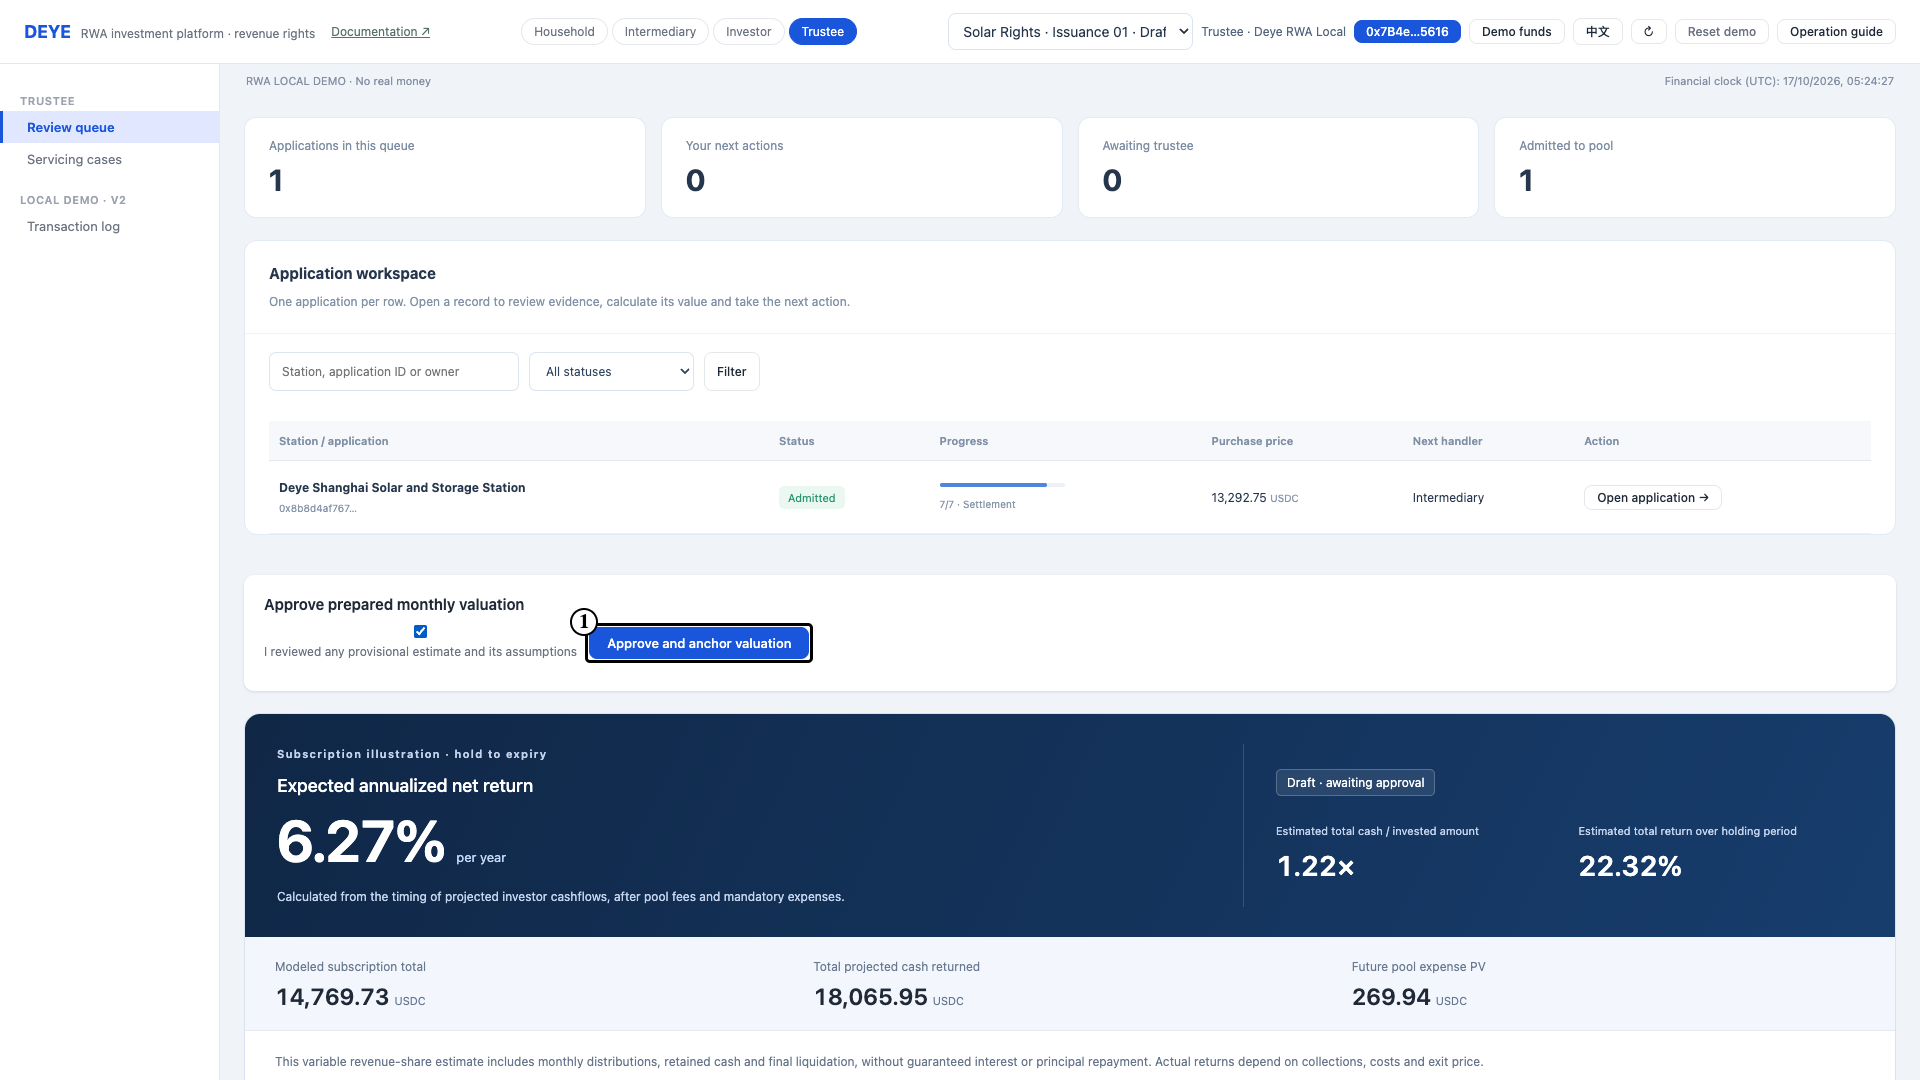
\includegraphics[width=\linewidth,height=.56\textheight,keepaspectratio]{assets/C5.en-context.png}\par Marker 1 identifies the control or information to inspect for this step. Amounts and dates refer to the isolated demonstration.\end{center}
\begin{center}
\includegraphics[width=.7\linewidth,height=1.55cm,keepaspectratio]{assets/C5.en-detail.png}\end{center}
\end{landscape}
\clearpage\begin{landscape}
\subsection{C6 Fundraising publication}
\label{step:C6}
This step is performed by Intermediary. Open Product operations and review projected net IRR, expected distributions, reserve policy, target, price and deadline. Publish the issuance terms with the wallet. Investors can then see the product as Fundraising, although no investor shares have been issued yet.

After this step, investors review the published product and apply for qualification.

\begin{center}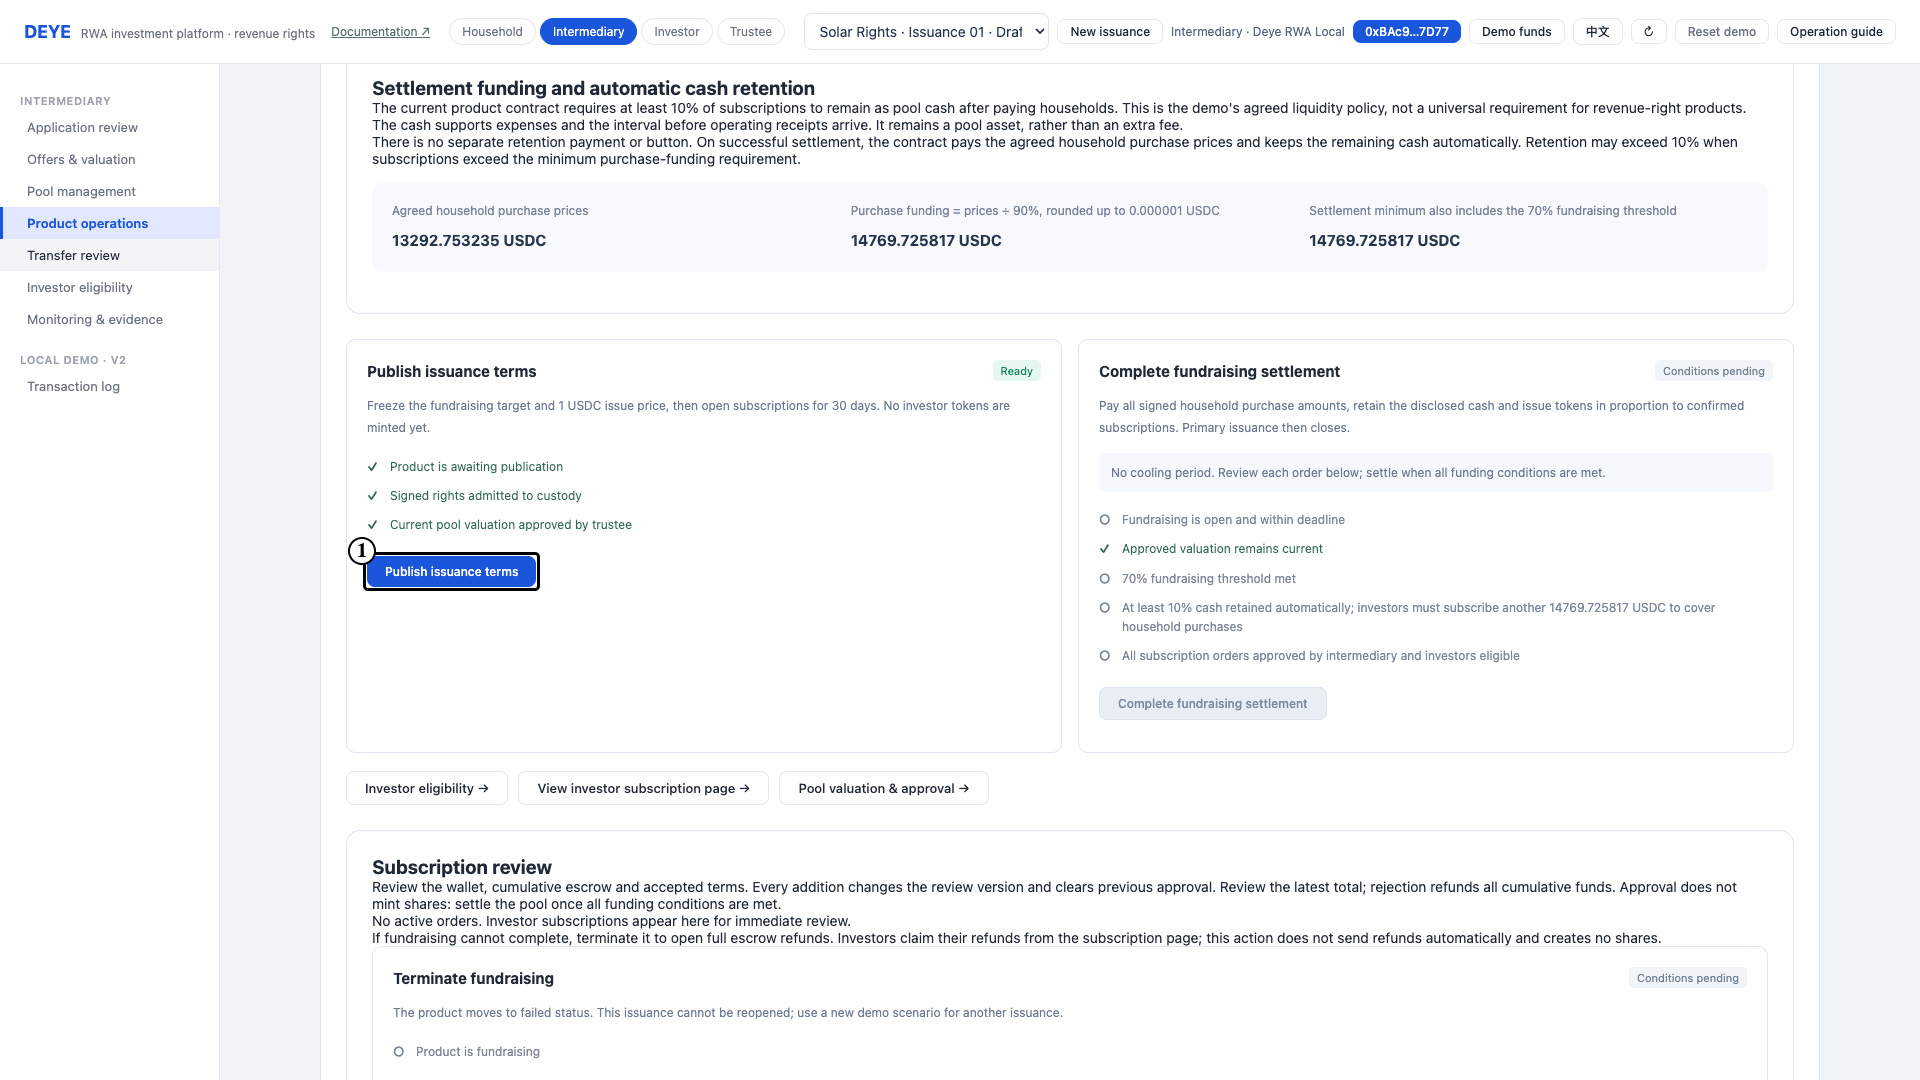
\includegraphics[width=\linewidth,height=.56\textheight,keepaspectratio]{assets/C6.en-context.png}\par Marker 1 identifies the control or information to inspect for this step. Amounts and dates refer to the isolated demonstration.\end{center}
\begin{center}
\includegraphics[width=.7\linewidth,height=1.55cm,keepaspectratio]{assets/C6.en-detail.png}\end{center}
\end{landscape}
\clearpage\begin{landscape}
\section{Qualification, subscriptions and settlement}
\subsection{D1 Product selection}
\label{step:D1}
This step is performed by Investor. Open Product hall and select a published Fundraising or Active product. Check its status, cadence, target and contract before entering details. Draft contracts are management work and are excluded from the investor hall.

After this step, review the product timeline and eligibility requirements.

\begin{center}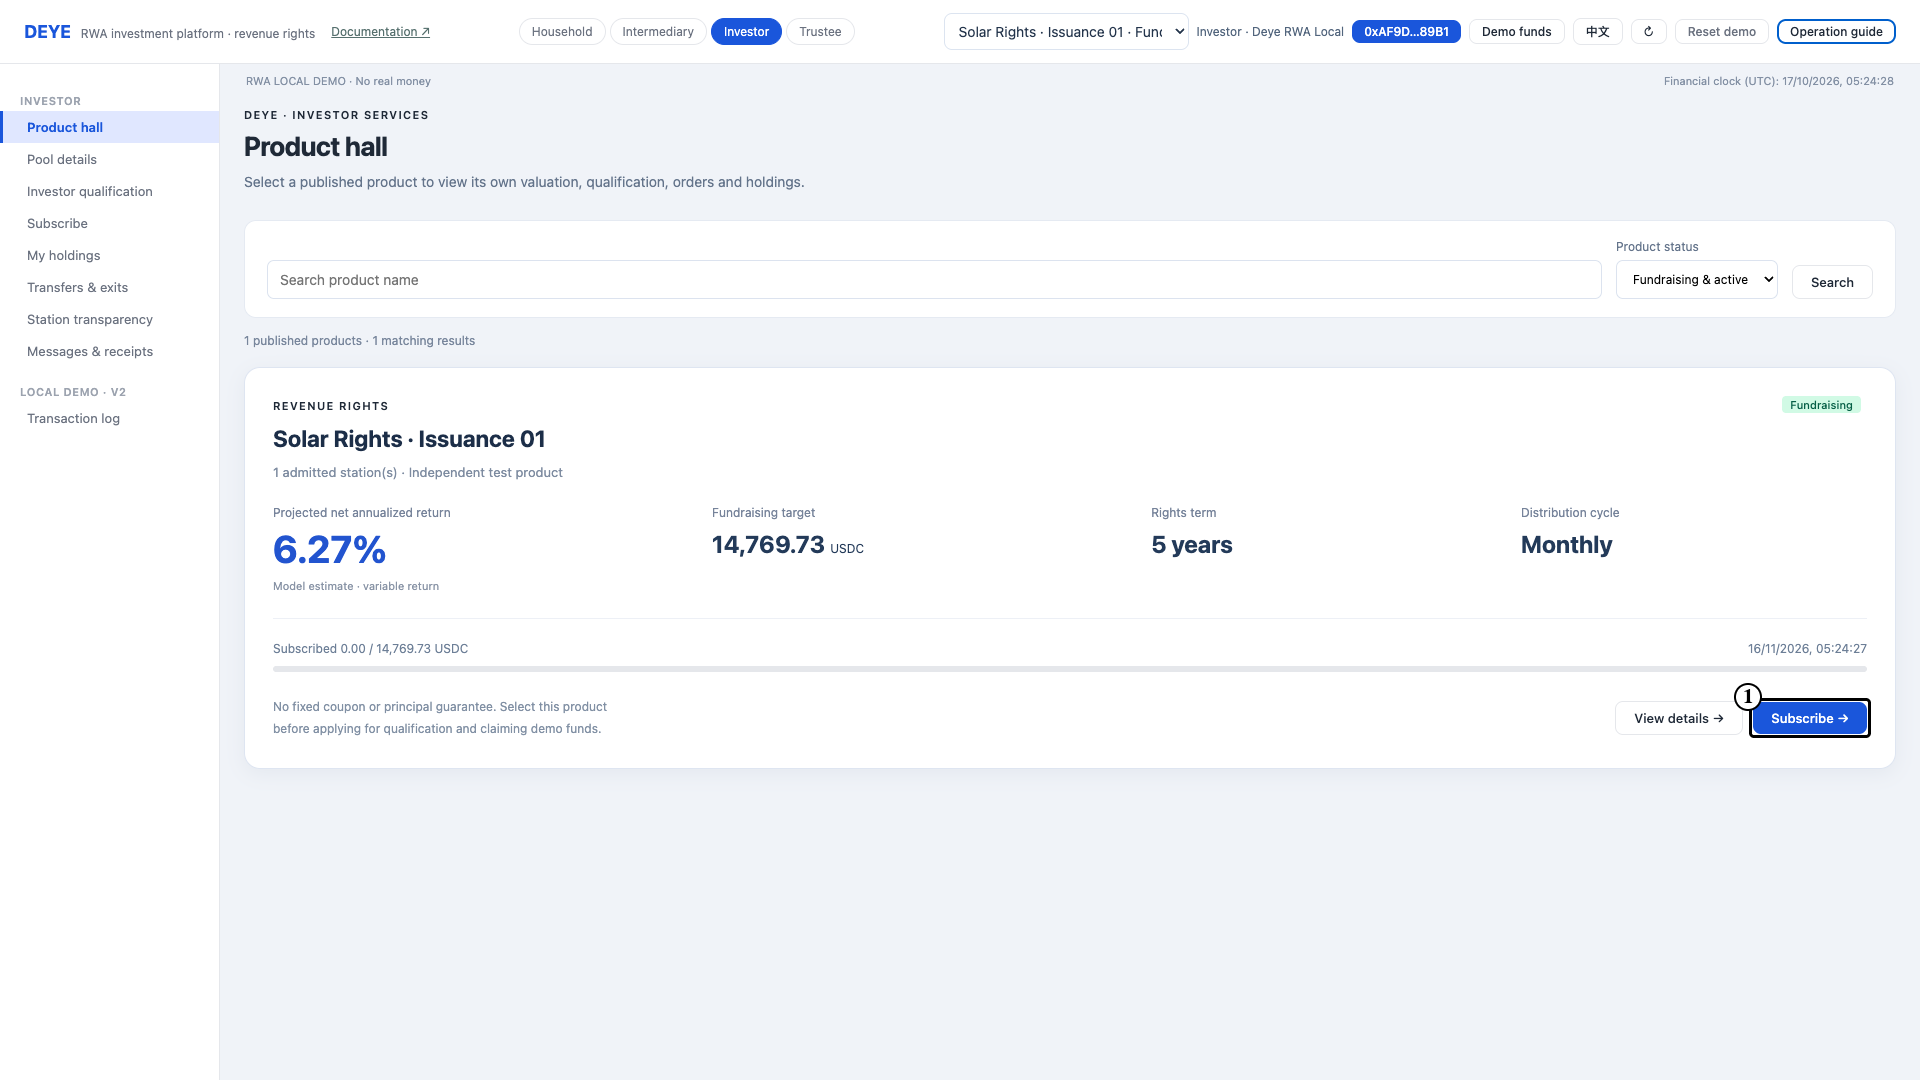
\includegraphics[width=\linewidth,height=.44\textheight,keepaspectratio]{assets/D1.en-context.png}\par Marker 1 identifies the control or information to inspect for this step. Amounts and dates refer to the isolated demonstration.\end{center}
\begin{center}
\includegraphics[width=.7\linewidth,height=1.55cm,keepaspectratio]{assets/D1.en-detail.png}\end{center}
\end{landscape}
\clearpage\begin{landscape}
\subsection{D2 Investor cashflow timeline}
\label{step:D2}
This step is performed by Investor. Read the monthly timeline in Pool details. Distinguish the initial investment, monthly collections, accrued expenses, declared distributions, retained cash and remaining NAV. The projected net IRR is a model result and is not the valuation discount rate or a guaranteed coupon.

After this step, apply for qualification before subscribing.

\begin{center}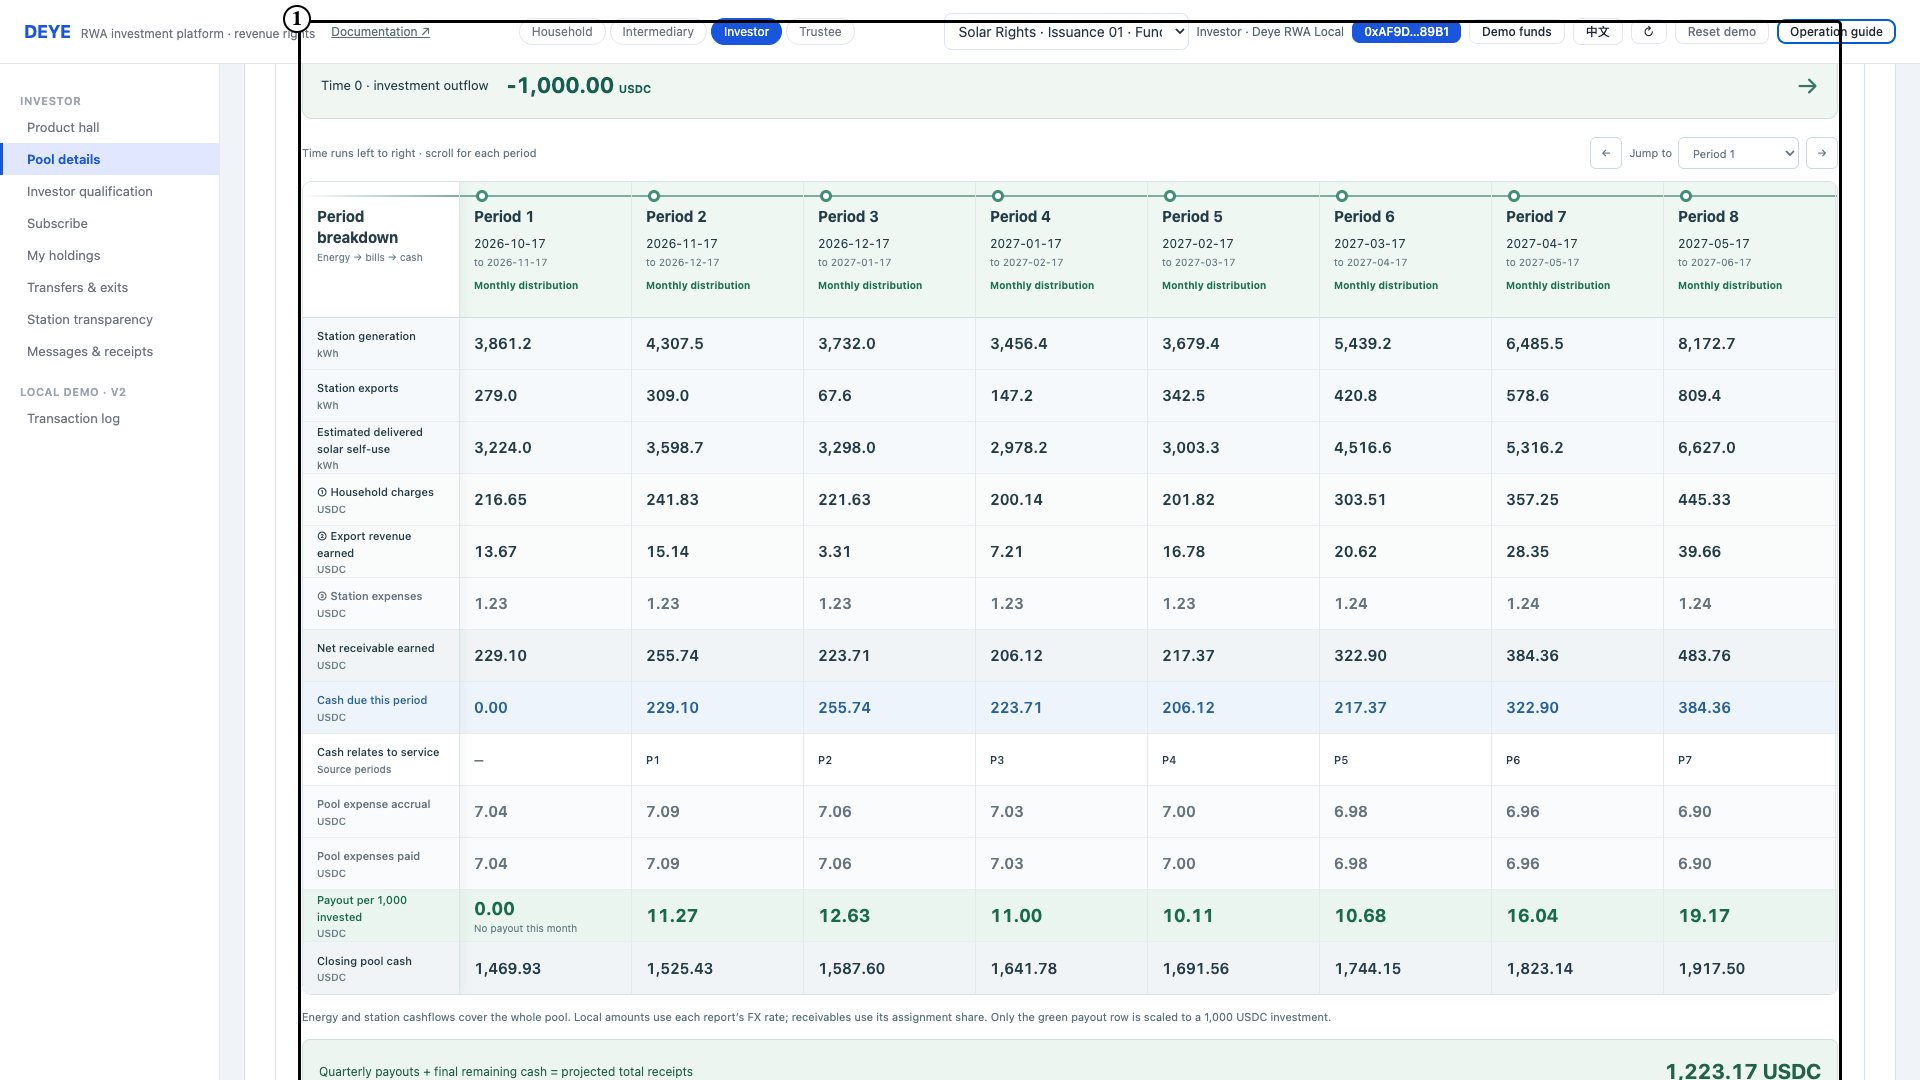
\includegraphics[width=\linewidth,height=.68\textheight,keepaspectratio]{assets/D2.en.png}\par Marker 1 identifies the control or information to inspect for this step. Amounts and dates refer to the isolated demonstration.\end{center}
\end{landscape}
\clearpage\begin{landscape}
\subsection{D3 Investment qualification application}
\label{step:D3}
This step is performed by Investor. Open Investment qualification, read the risk statement and acknowledge the test-only setting. Submit the application for the connected wallet and selected product. A staff member must approve it before the contract accepts a subscription.

After this step, the intermediary reviews this wallet's qualification.

\begin{center}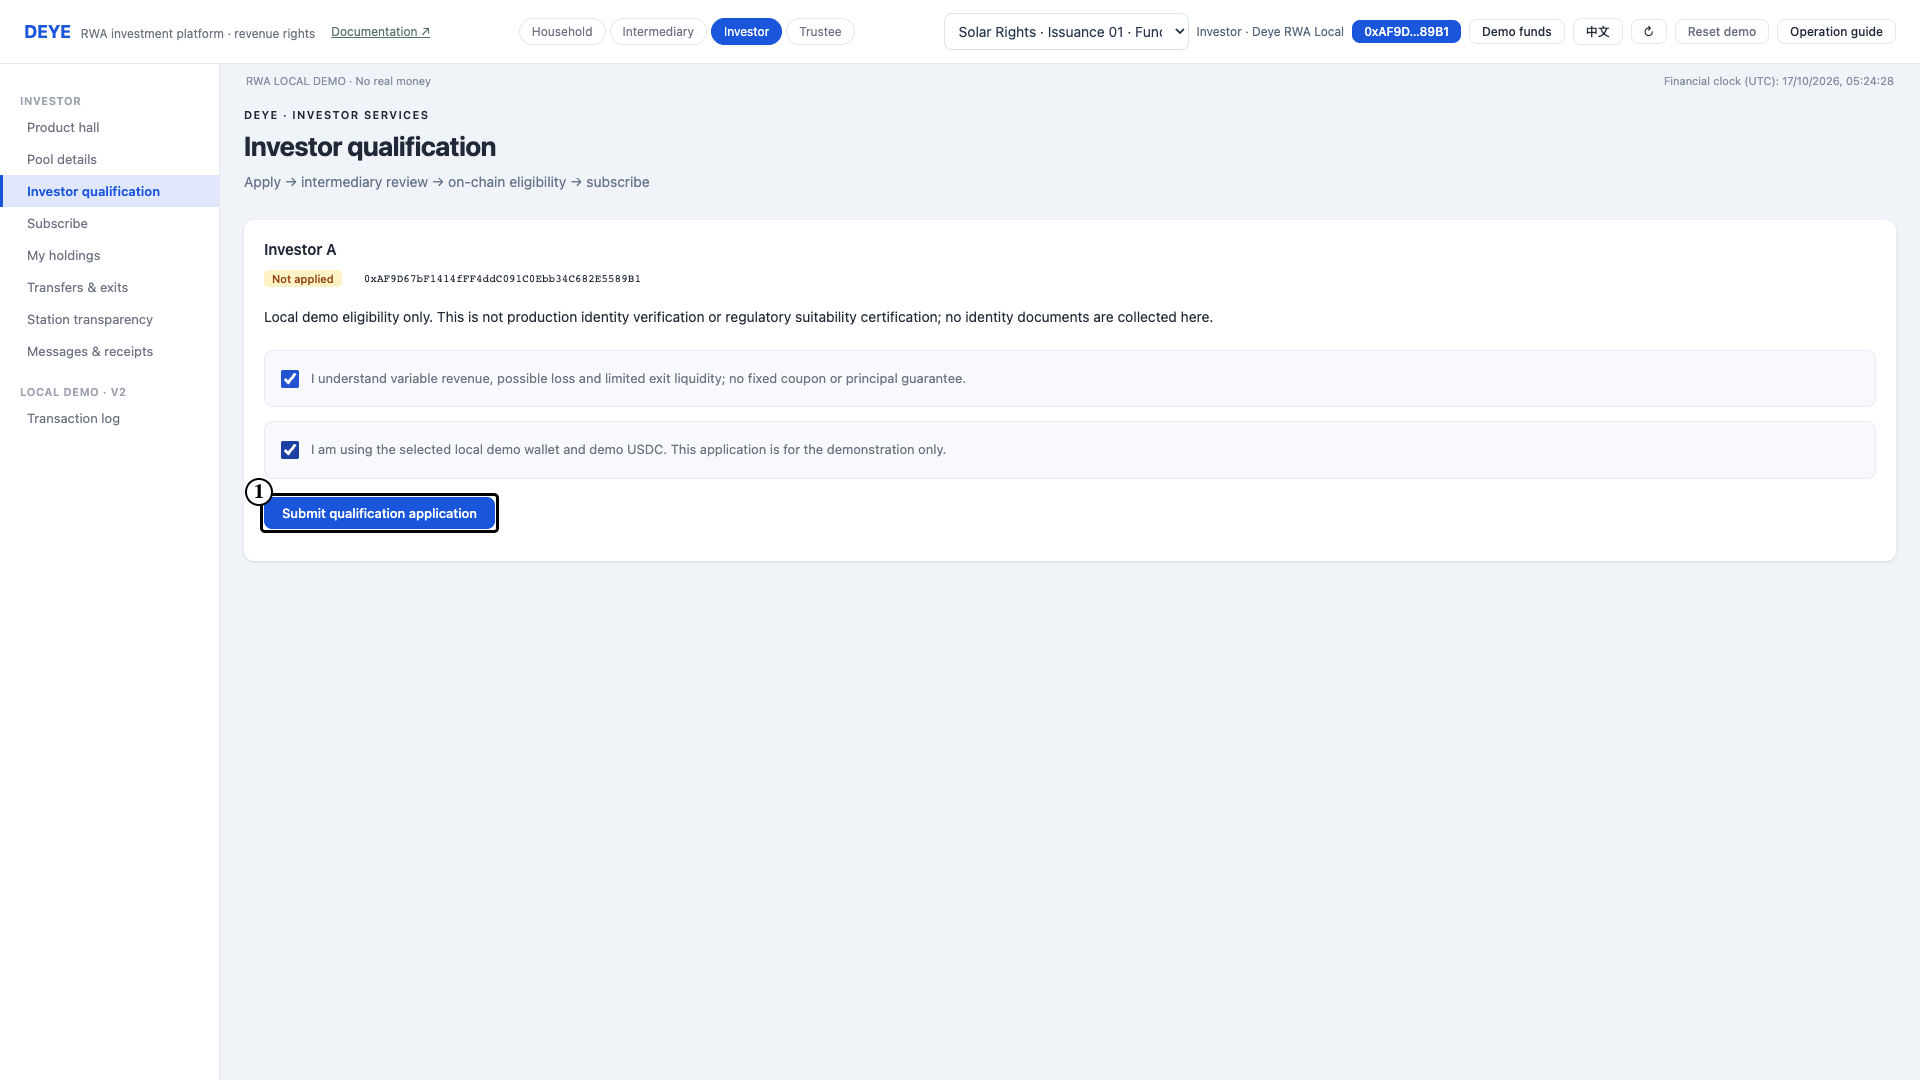
\includegraphics[width=\linewidth,height=.56\textheight,keepaspectratio]{assets/D3.en-context.png}\par Marker 1 identifies the control or information to inspect for this step. Amounts and dates refer to the isolated demonstration.\end{center}
\begin{center}
\includegraphics[width=.7\linewidth,height=1.55cm,keepaspectratio]{assets/D3.en-detail.png}\end{center}
\end{landscape}
\clearpage\begin{landscape}
\subsection{D4 Qualification approval}
\label{step:D4}
This step is performed by Intermediary. Open the qualification queue, select the investor and review the application. Approve the correct wallet for the selected product and confirm the on-chain transaction. Choosing an investor role in the UI does not grant eligibility.

After this step, the investor receives test funds and submits a subscription.

\begin{center}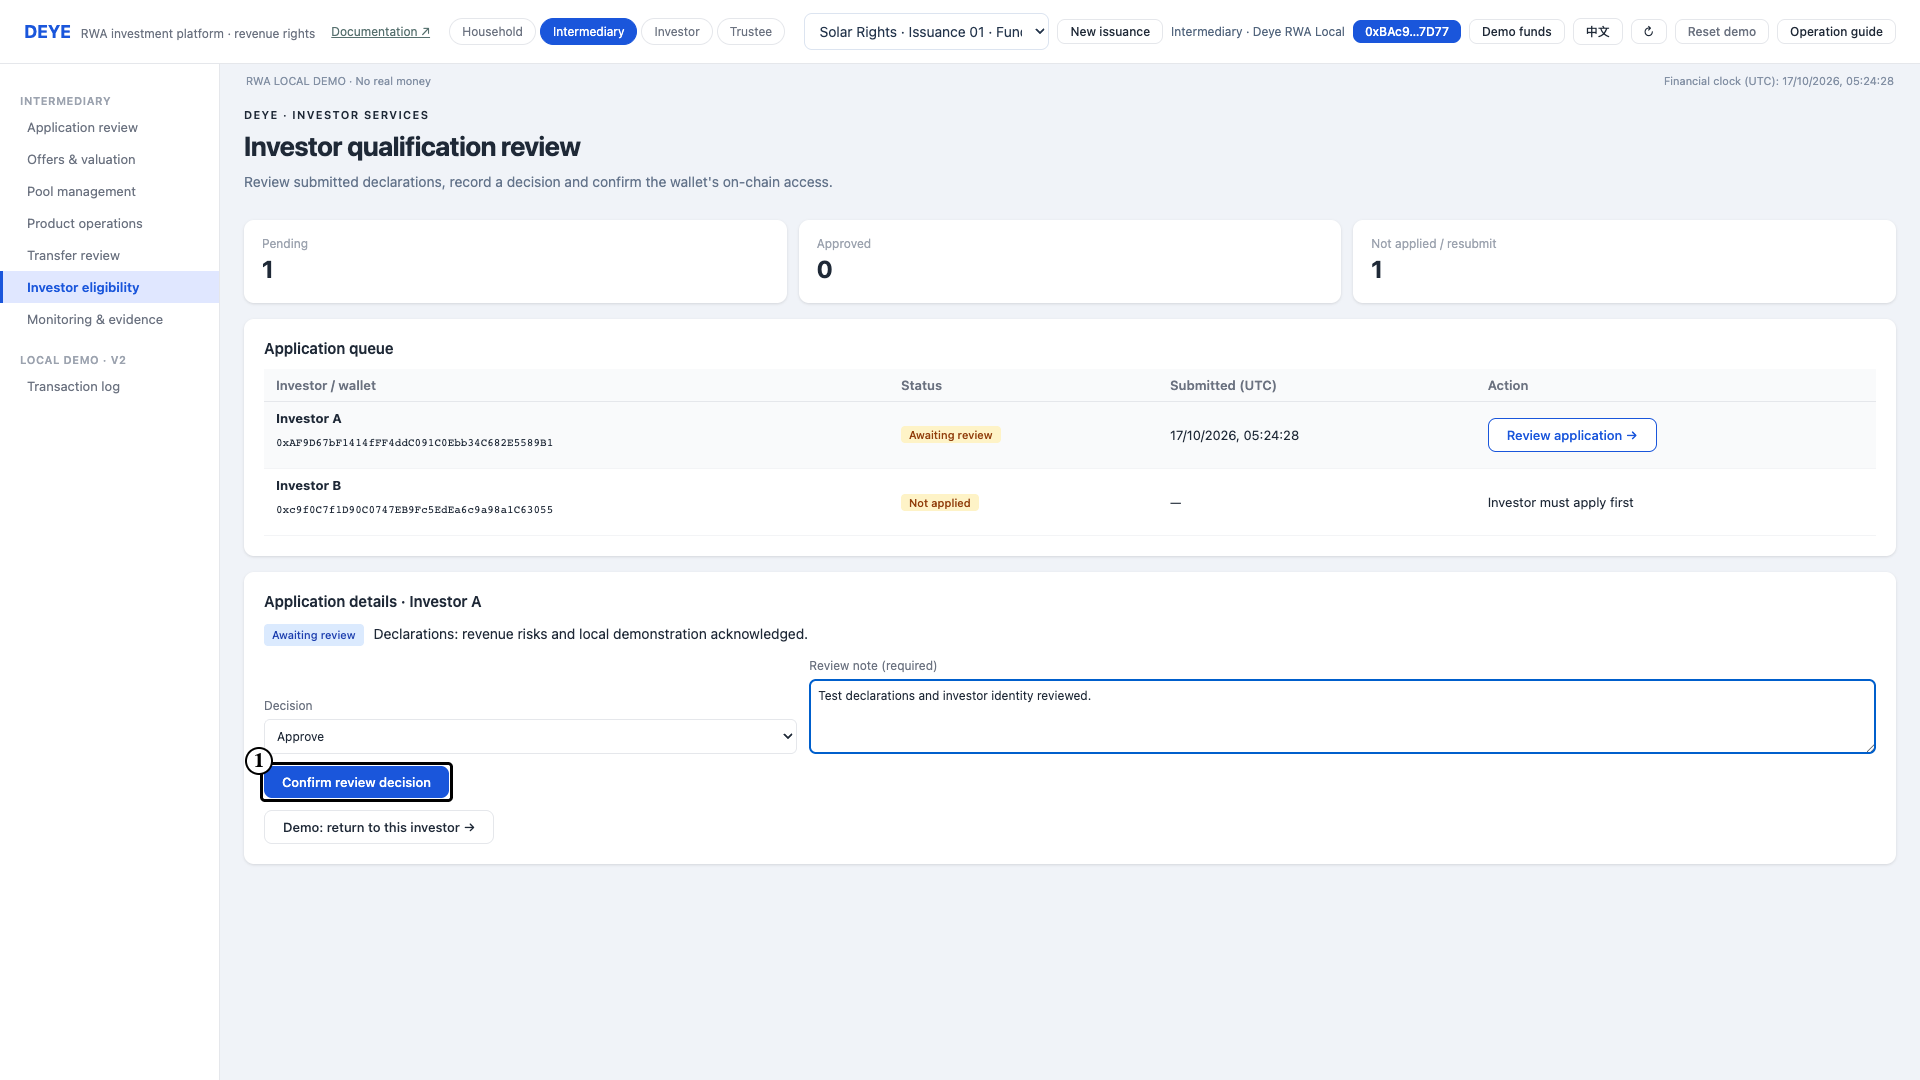
\includegraphics[width=\linewidth,height=.56\textheight,keepaspectratio]{assets/D4.en-context.png}\par Marker 1 identifies the control or information to inspect for this step. Amounts and dates refer to the isolated demonstration.\end{center}
\begin{center}
\includegraphics[width=.7\linewidth,height=1.55cm,keepaspectratio]{assets/D4.en-detail.png}\end{center}
\end{landscape}
\clearpage\begin{landscape}
\subsection{D5 USDC approval and subscription}
\label{step:D5}
This step is performed by Investor. Enter the additional amount in Subscription and check the remaining capacity and wallet balance. Confirm USDC approval if requested, then confirm the subscription transaction. Each addition increases cumulative escrow and invalidates the earlier order review. Repeat subscriptions remain available while fundraising permits them.

After this step, the intermediary reviews the latest cumulative amount before settlement.

\begin{center}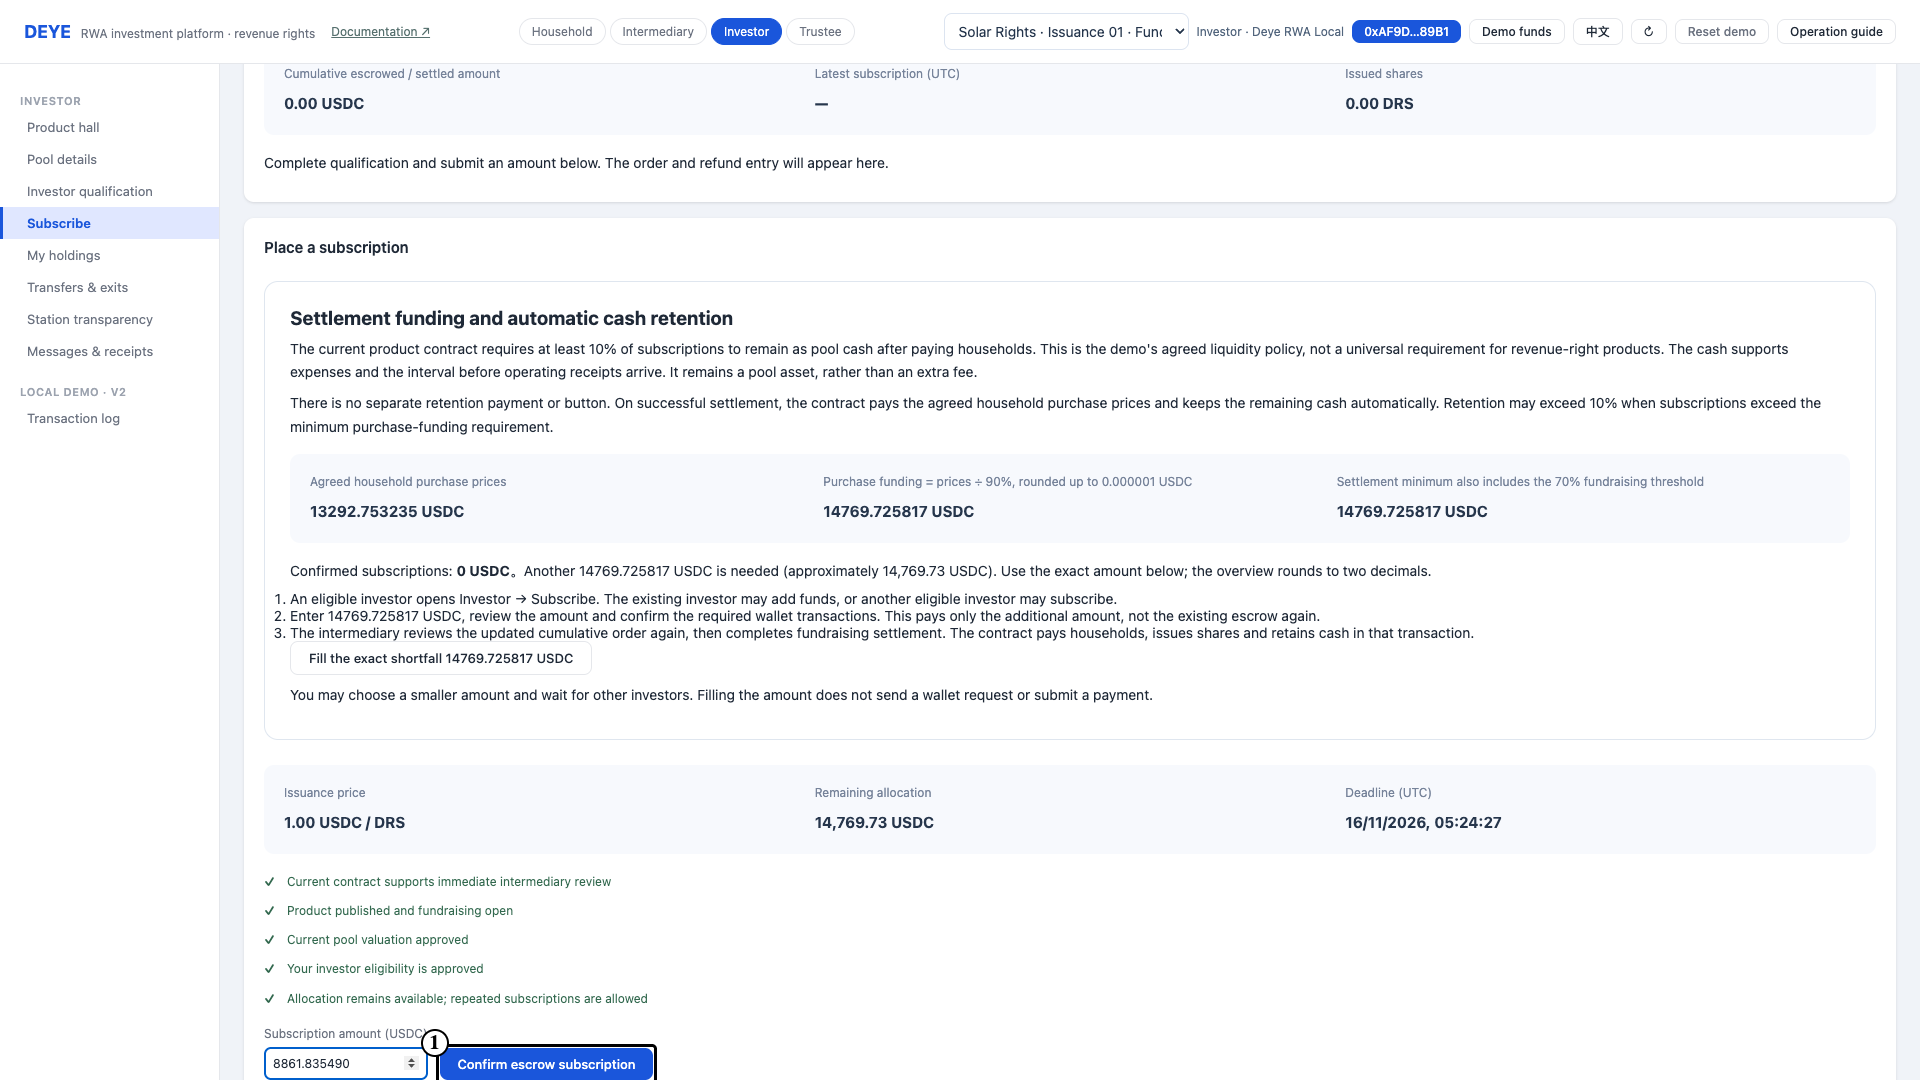
\includegraphics[width=\linewidth,height=.56\textheight,keepaspectratio]{assets/D5.en-context.png}\par Marker 1 identifies the control or information to inspect for this step. Amounts and dates refer to the isolated demonstration.\end{center}
\begin{center}
\includegraphics[width=.7\linewidth,height=1.55cm,keepaspectratio]{assets/D5.en-detail.png}\end{center}
\end{landscape}
\clearpage\begin{landscape}
\subsection{D6 Cancellation before settlement}
\label{step:D6}
This step is performed by Investor. Open the order and click the refund action before issuance settlement. Confirm the wallet transaction and check that the full cumulative escrow returns to the wallet. This cancels the pending investment without issuing DRS.

After this step, the investor may subscribe again while fundraising remains open.

\begin{center}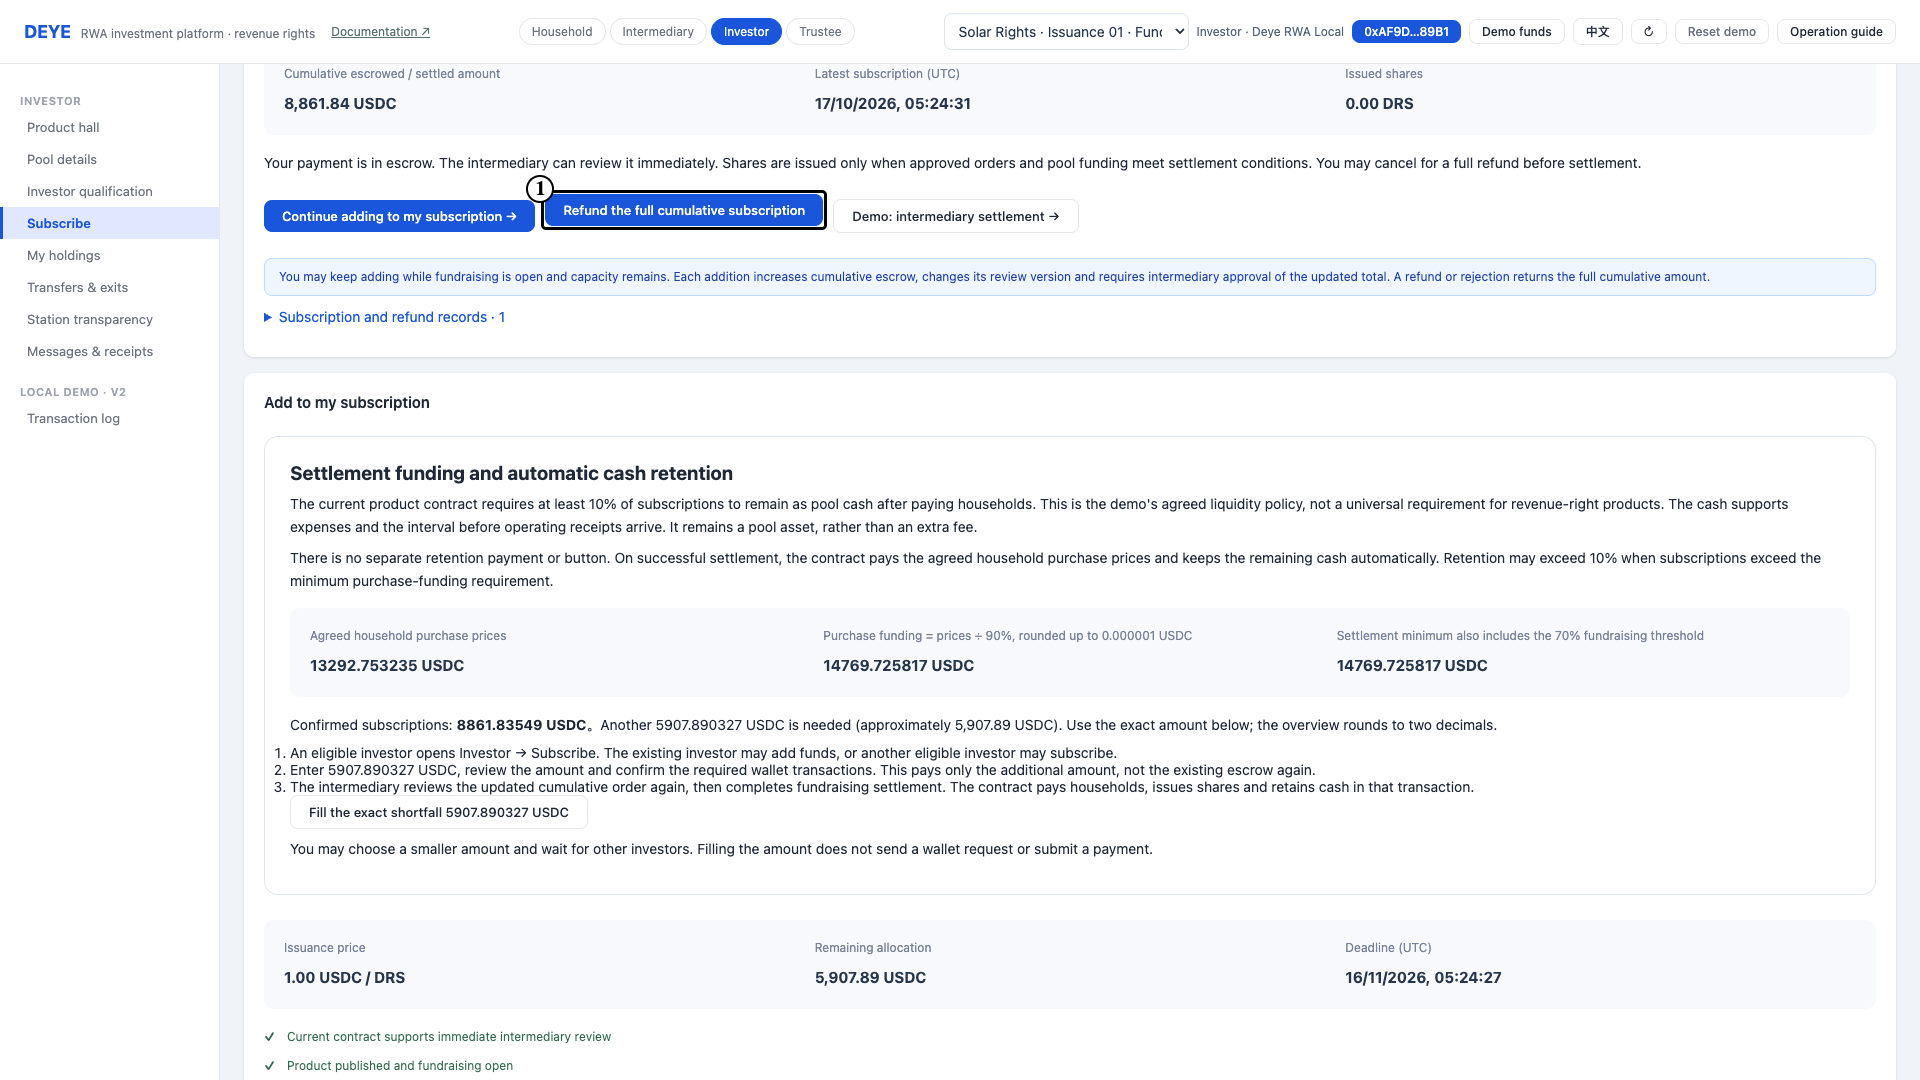
\includegraphics[width=\linewidth,height=.56\textheight,keepaspectratio]{assets/D6.en-context.png}\par Marker 1 identifies the control or information to inspect for this step. Amounts and dates refer to the isolated demonstration.\end{center}
\begin{center}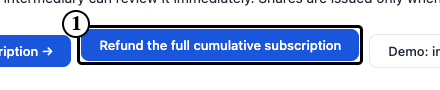
\includegraphics[width=.7\linewidth,height=1.55cm,keepaspectratio]{assets/D6.en-detail.png}\end{center}
\end{landscape}
\clearpage\begin{landscape}
\subsection{D7 Cumulative subscription review}
\label{step:D7}
This step is performed by Intermediary. In Product operations, locate the investor's order and compare wallet, cumulative escrow and issuance terms. Approve the latest review version with the intermediary wallet. Approval does not issue shares, and a later addition requires another review.

After this step, settle only when every order and all funding conditions are satisfied.

\begin{center}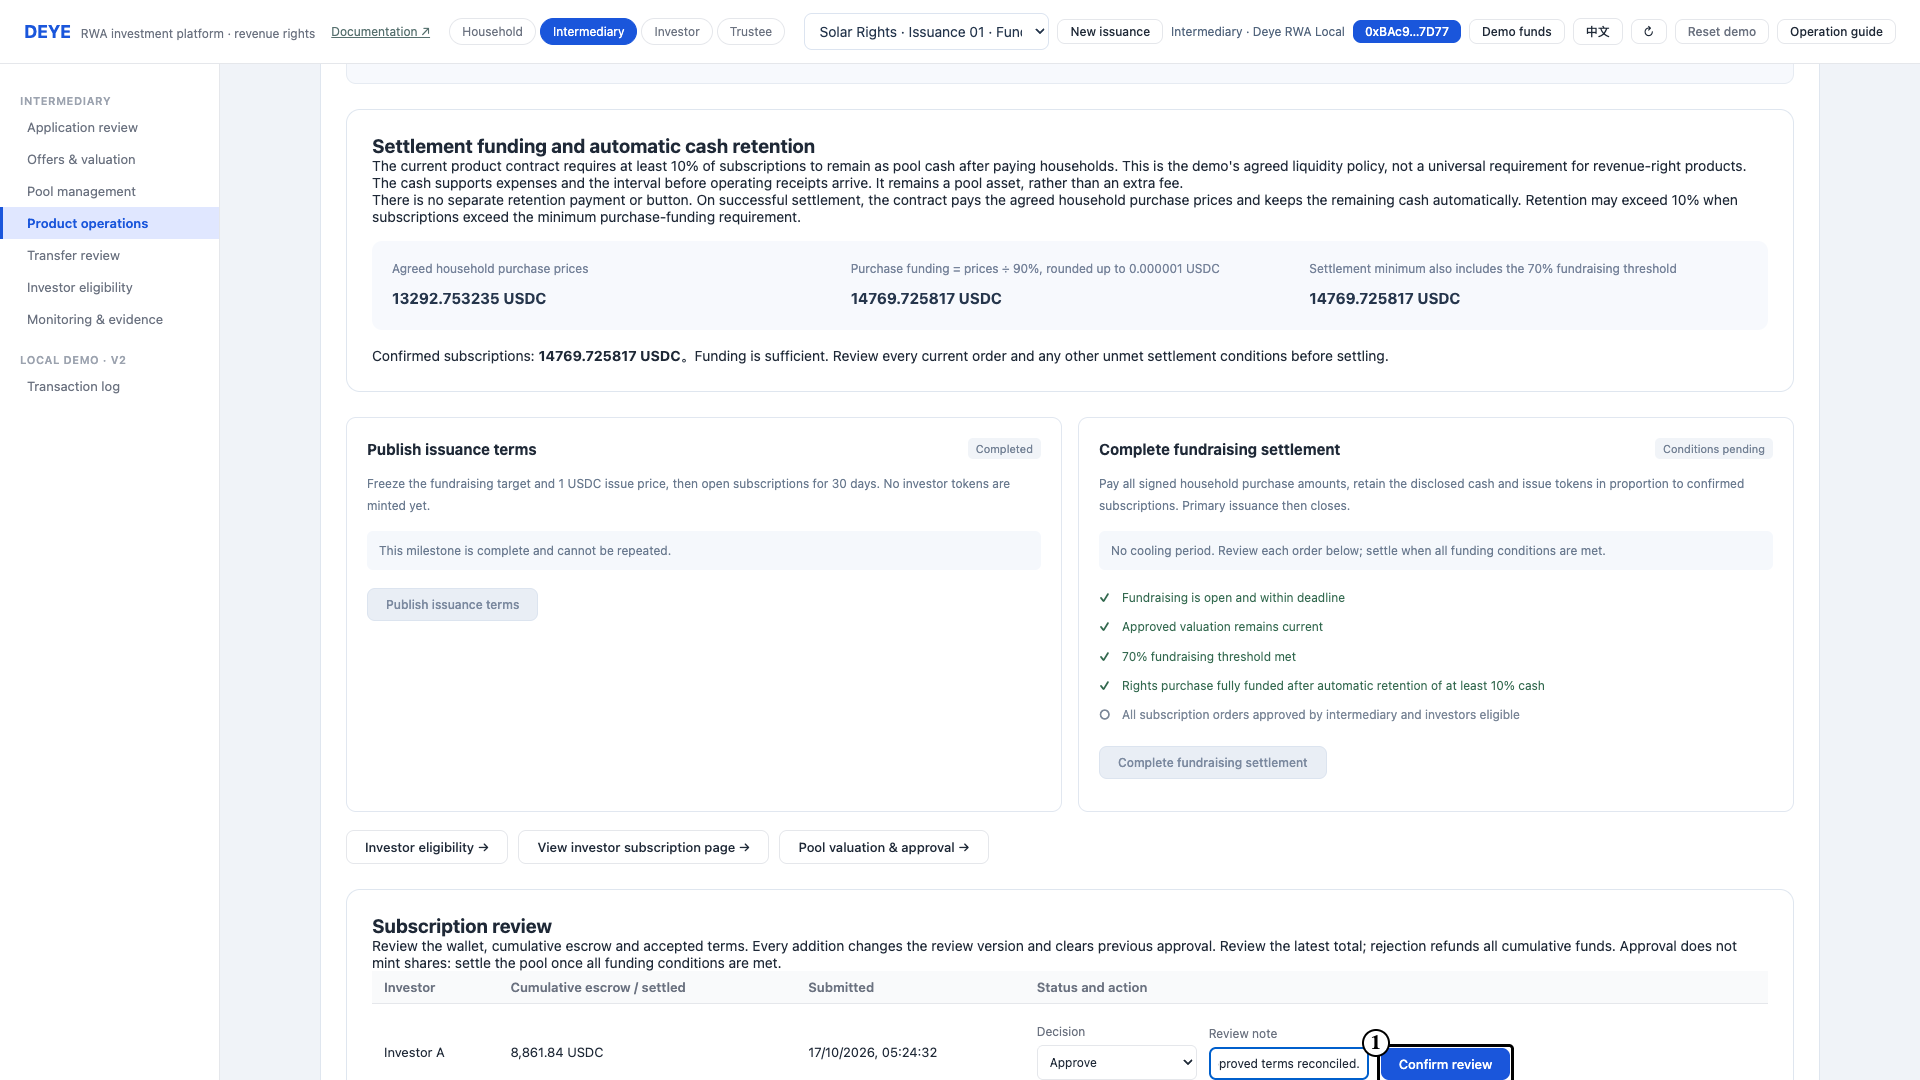
\includegraphics[width=\linewidth,height=.56\textheight,keepaspectratio]{assets/D7.en-context.png}\par Marker 1 identifies the control or information to inspect for this step. Amounts and dates refer to the isolated demonstration.\end{center}
\begin{center}
\includegraphics[width=.7\linewidth,height=1.55cm,keepaspectratio]{assets/D7.en-detail.png}\end{center}
\end{landscape}
\clearpage\begin{landscape}
\subsection{D8 Fundraising settlement and share issuance}
\label{step:D8}
This step is performed by Intermediary. Check that all orders are approved and the subscription total covers signed purchases plus the 10\% initial cash retention. The contract retains the cash automatically during settlement. If a shortfall is shown, direct the investor to add exactly that amount and review the updated order before settling.

After this step, the owner receives the purchase payment and investors inspect their issued shares.

\begin{center}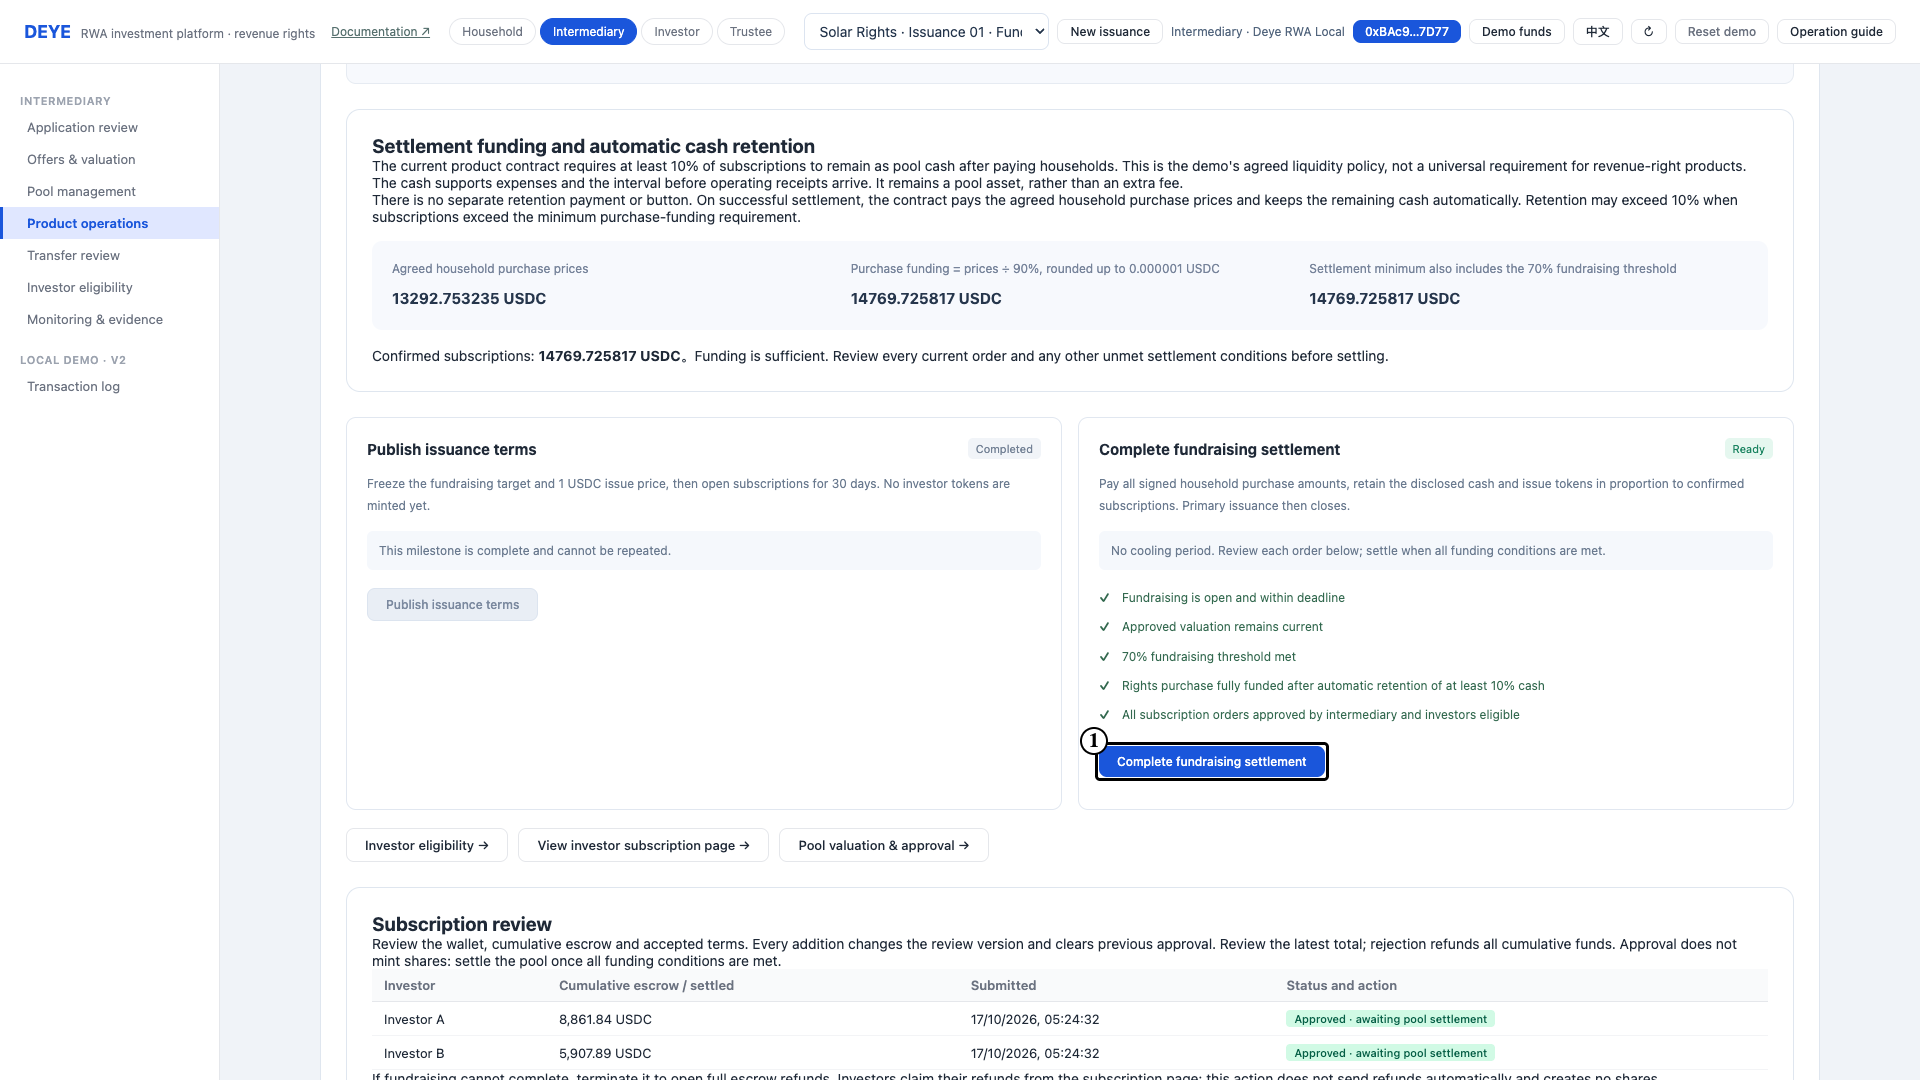
\includegraphics[width=\linewidth,height=.56\textheight,keepaspectratio]{assets/D8.en-context.png}\par Marker 1 identifies the control or information to inspect for this step. Amounts and dates refer to the isolated demonstration.\end{center}
\begin{center}
\includegraphics[width=.7\linewidth,height=1.55cm,keepaspectratio]{assets/D8.en-detail.png}\end{center}
\end{landscape}
\clearpage\begin{landscape}
\subsection{D9 Confirmed investment position}
\label{step:D9}
This step is performed by Investor. Open My holdings after settlement and refresh the confirmed state. Check DRS, the settlement record, the latest approved NAV and any declared distribution. Wallet USDC, subscription escrow and investment NAV are different amounts.

After this step, the intermediary begins monthly collection and accounting.

\begin{center}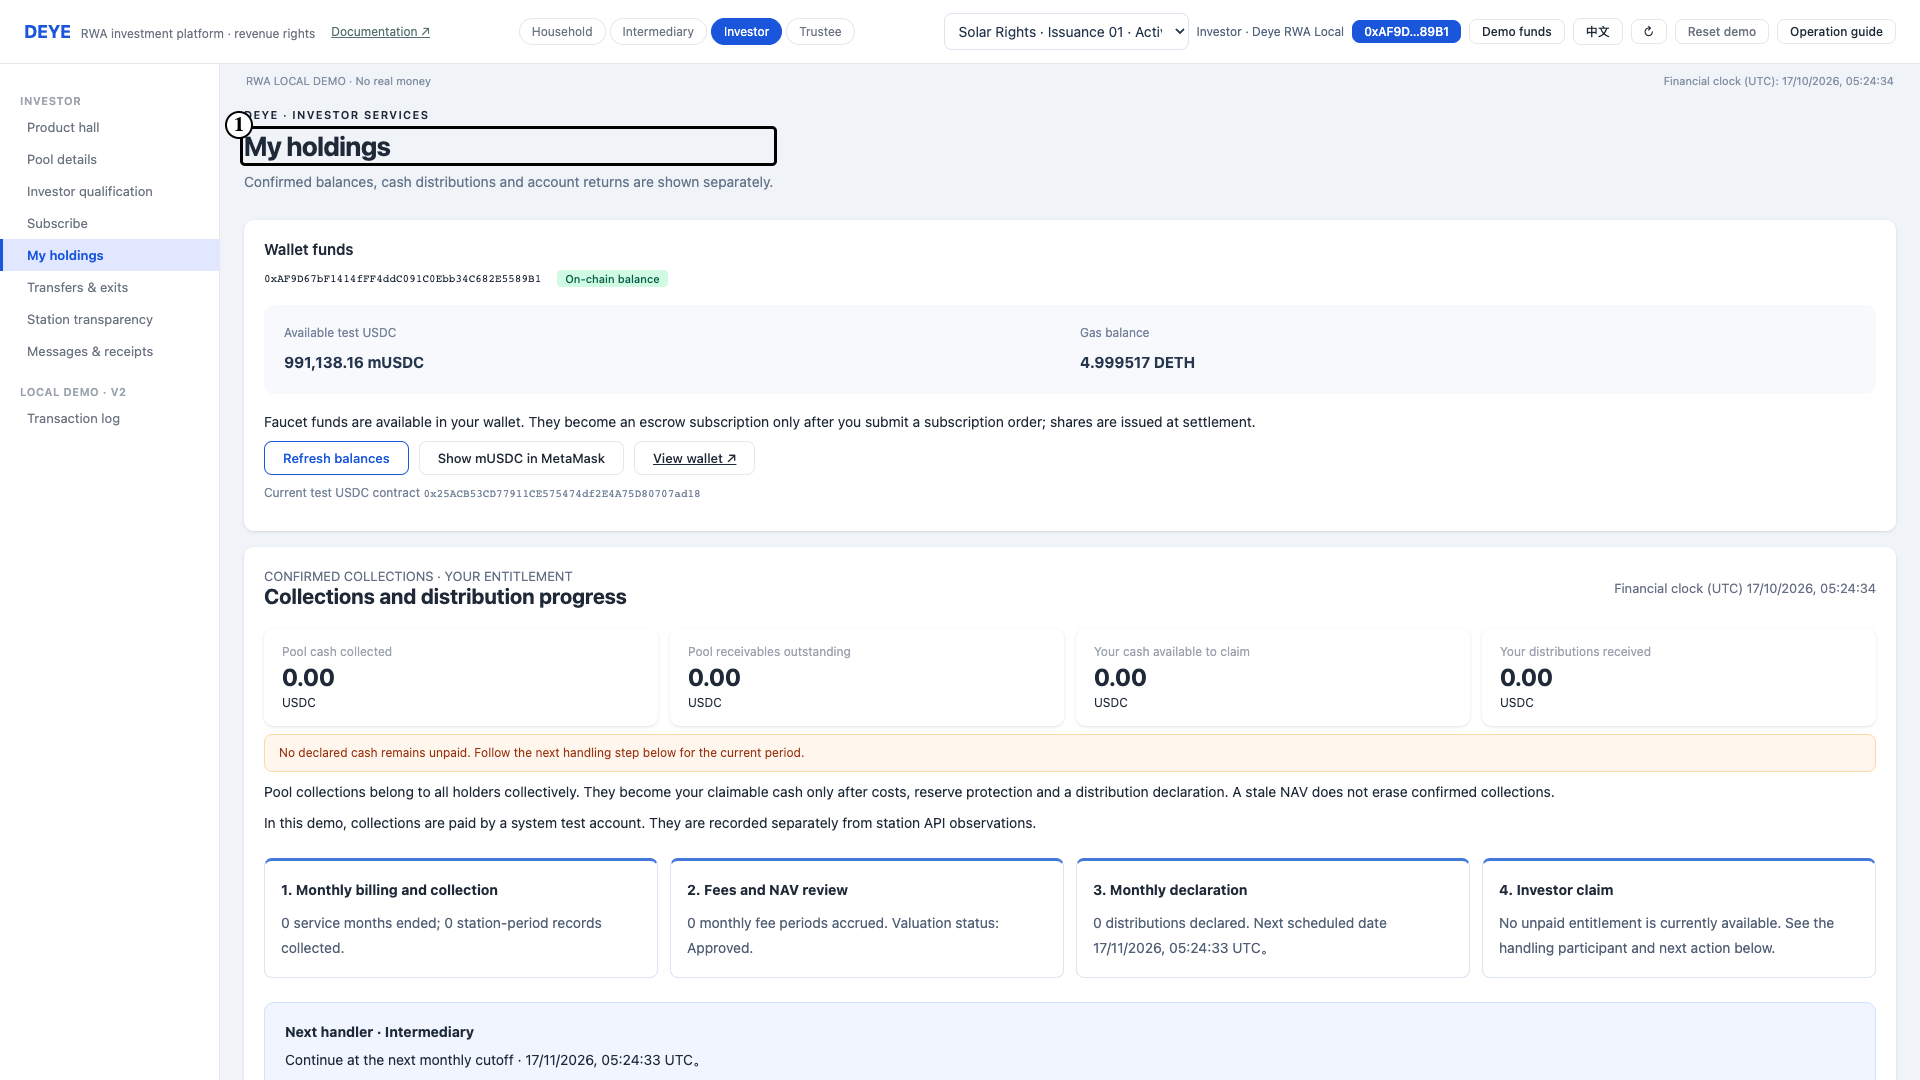
\includegraphics[width=\linewidth,height=.56\textheight,keepaspectratio]{assets/D9.en-context.png}\par Marker 1 identifies the control or information to inspect for this step. Amounts and dates refer to the isolated demonstration.\end{center}
\begin{center}
\includegraphics[width=.7\linewidth,height=1.55cm,keepaspectratio]{assets/D9.en-detail.png}\end{center}
\end{landscape}
\clearpage\begin{landscape}
\section{Monthly collections, valuation and distributions}
\subsection{E1 Demonstration financial cutoff}
\label{step:E1}
This step is performed by Intermediary. Use Locate operation for the monthly fee task. If its cutoff has not arrived, choose the offered financial-time shortcut and read the shared-clock confirmation. Advancing the test clock affects all products on the chain and does not create live telemetry or approve valuations.

After this step, record completed service periods and reconcile the opening NAV before accruing fees.

\begin{center}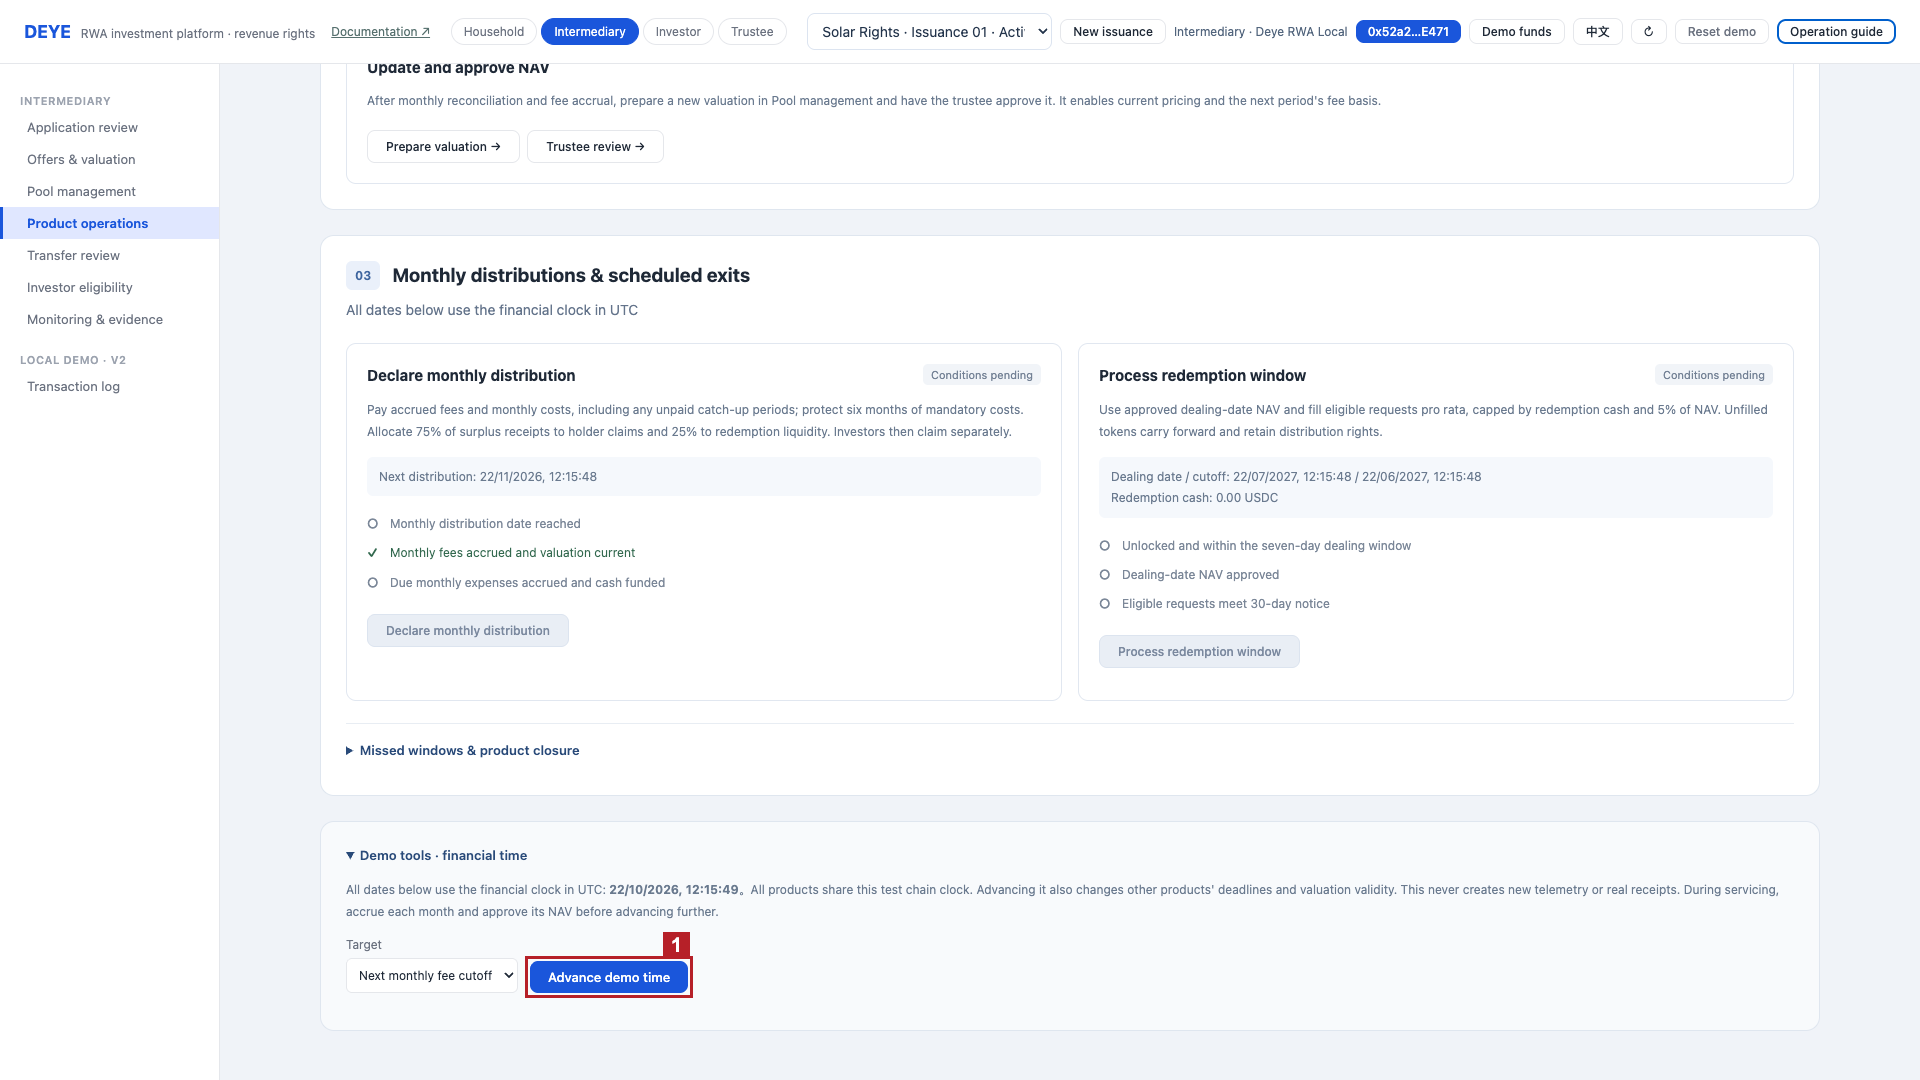
\includegraphics[width=\linewidth,height=.44\textheight,keepaspectratio]{assets/E1.en-context.png}\par Marker 1 identifies the control or information to inspect for this step. Amounts and dates refer to the isolated demonstration.\end{center}
\begin{center}
\includegraphics[width=.7\linewidth,height=1.55cm,keepaspectratio]{assets/E1.en-detail.png}\end{center}
\end{landscape}
\clearpage\begin{landscape}
\subsection{E2 Publish the monthly payment bill}
\label{step:E2}
This step is performed by Intermediary. Under Monitoring \& evidence, check the service period and complete recorded history month. Review the household bill, export income, station costs and FX, then use marker 1 to publish and confirm the wallet transaction.

After this step, the invoice binds the designated household, exact test-USDC payment and evidence digest. No cash has been collected yet. The owner pays next.

\begin{center}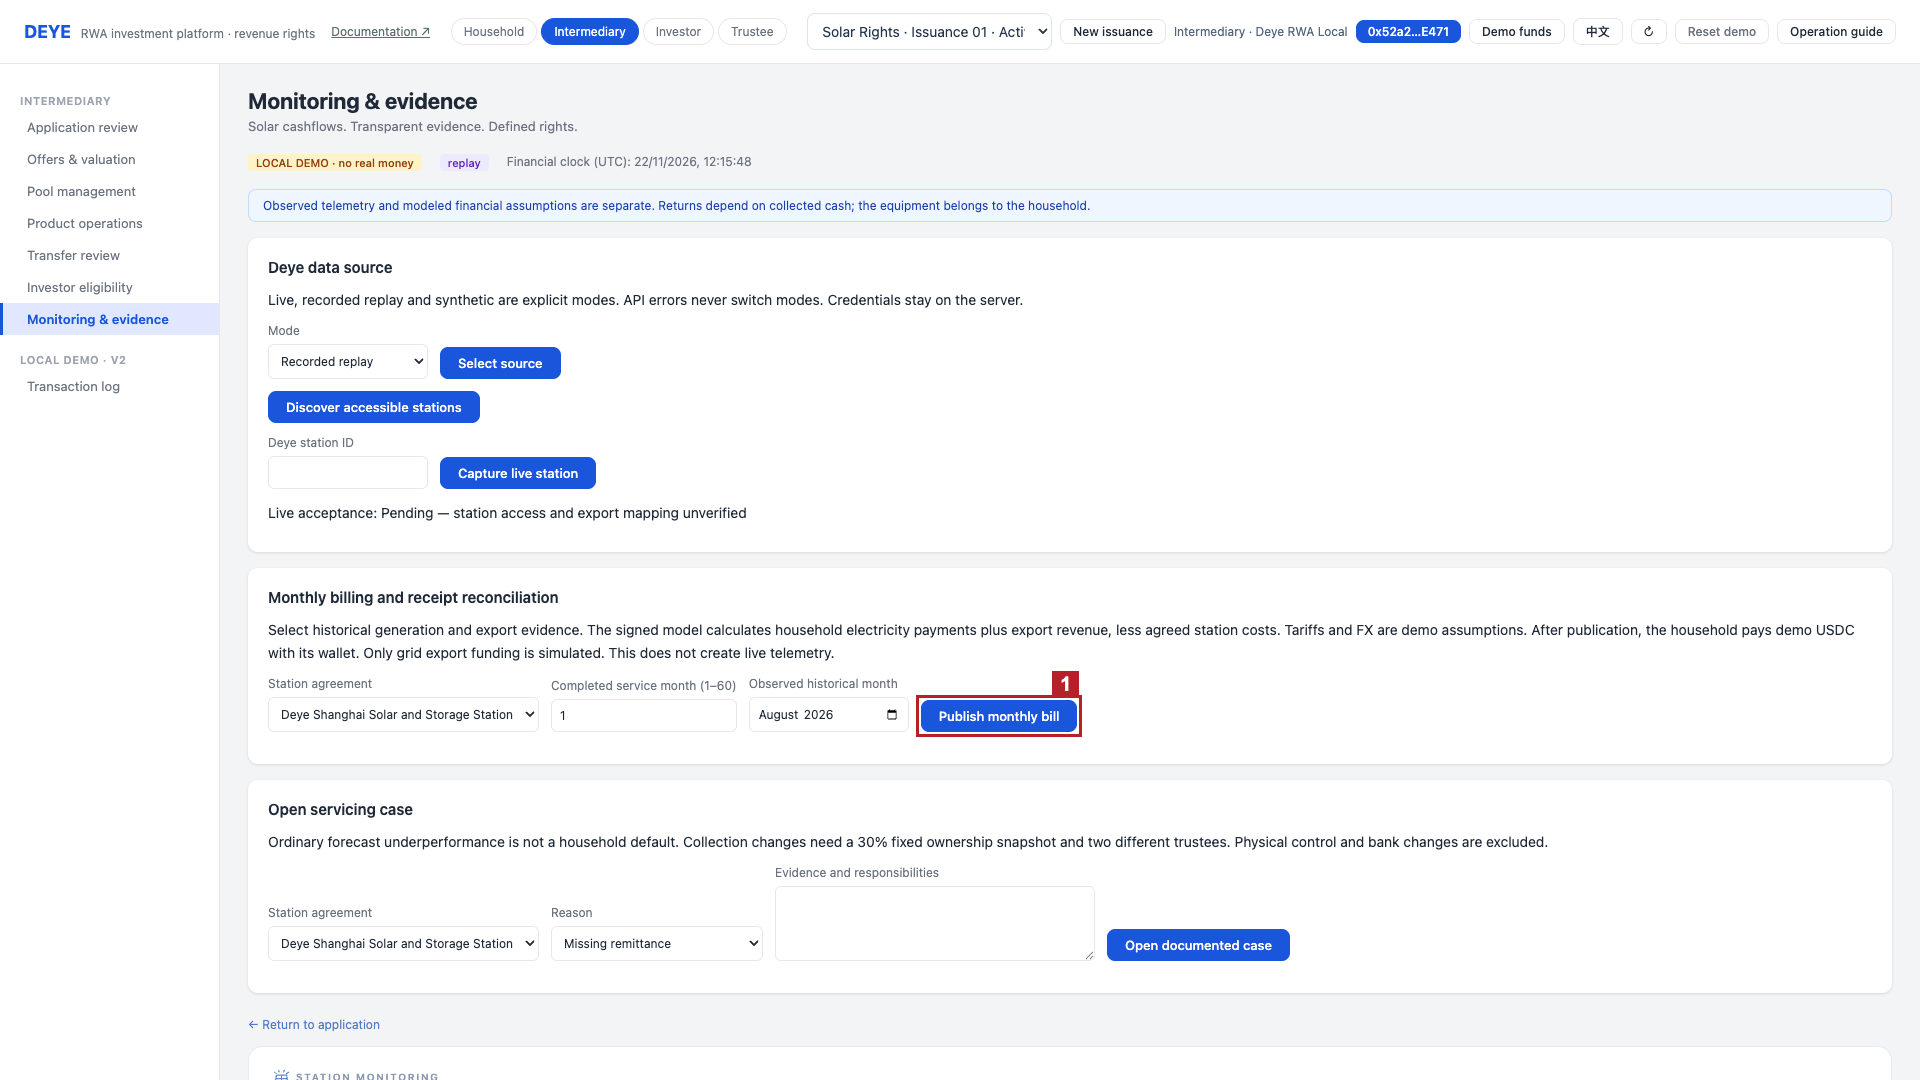
\includegraphics[width=\linewidth,height=.56\textheight,keepaspectratio]{assets/E2.en-context.png}\par Marker 1 identifies the control or information to inspect for this step. Amounts and dates refer to the isolated demonstration.\end{center}
\begin{center}
\includegraphics[width=.7\linewidth,height=1.55cm,keepaspectratio]{assets/E2.en-detail.png}\end{center}
\end{landscape}
\clearpage\begin{landscape}
\subsection{E3 Approve and pay the monthly bill}
\label{step:E3}
This step is performed by Owner. Under Funds \& monthly bills, check the product, period, token and amount. Use marker 1, approve the exact invoice amount in the wallet and then confirm payment. Explicitly claim test funds first if the balance is insufficient.

After this step, the household wallet transfers the bill amount into the billing contract. The invoice awaits intermediary reconciliation. A direct token transfer does not settle a named bill.

\begin{center}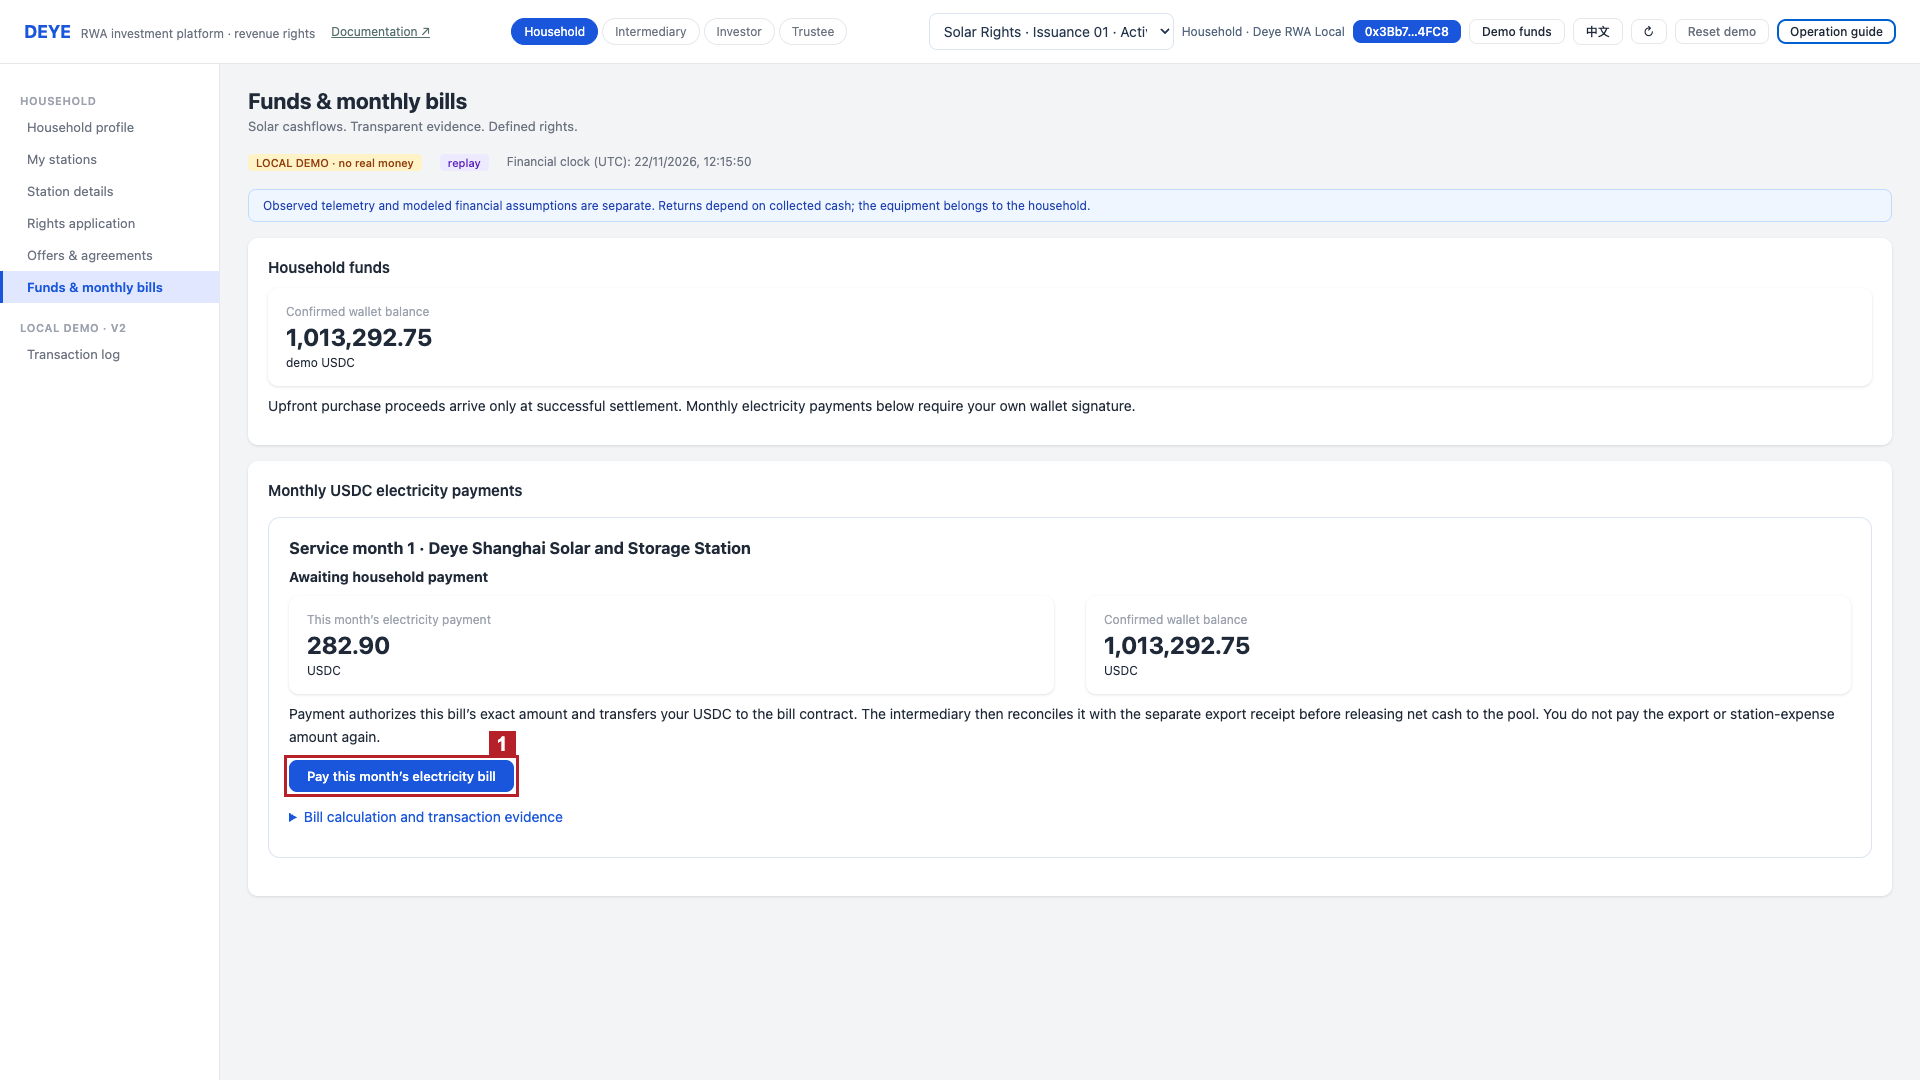
\includegraphics[width=\linewidth,height=.56\textheight,keepaspectratio]{assets/E3.en-context.png}\par Marker 1 identifies the control or information to inspect for this step. Amounts and dates refer to the isolated demonstration.\end{center}
\begin{center}
\includegraphics[width=.7\linewidth,height=1.55cm,keepaspectratio]{assets/E3.en-detail.png}\end{center}
\end{landscape}
\clearpage\begin{landscape}
\subsection{E3a Record the separate grid-export receipt}
\label{step:E3a}
This step is performed by Intermediary. Under Monitoring \& evidence, inspect the same invoice and household-payment status. Use marker 1 to record only the explicitly simulated grid-export receipt.

After this step, a separate system account funds the export component. It does not replace or top up the household payment. Both components await reconciliation.

\begin{center}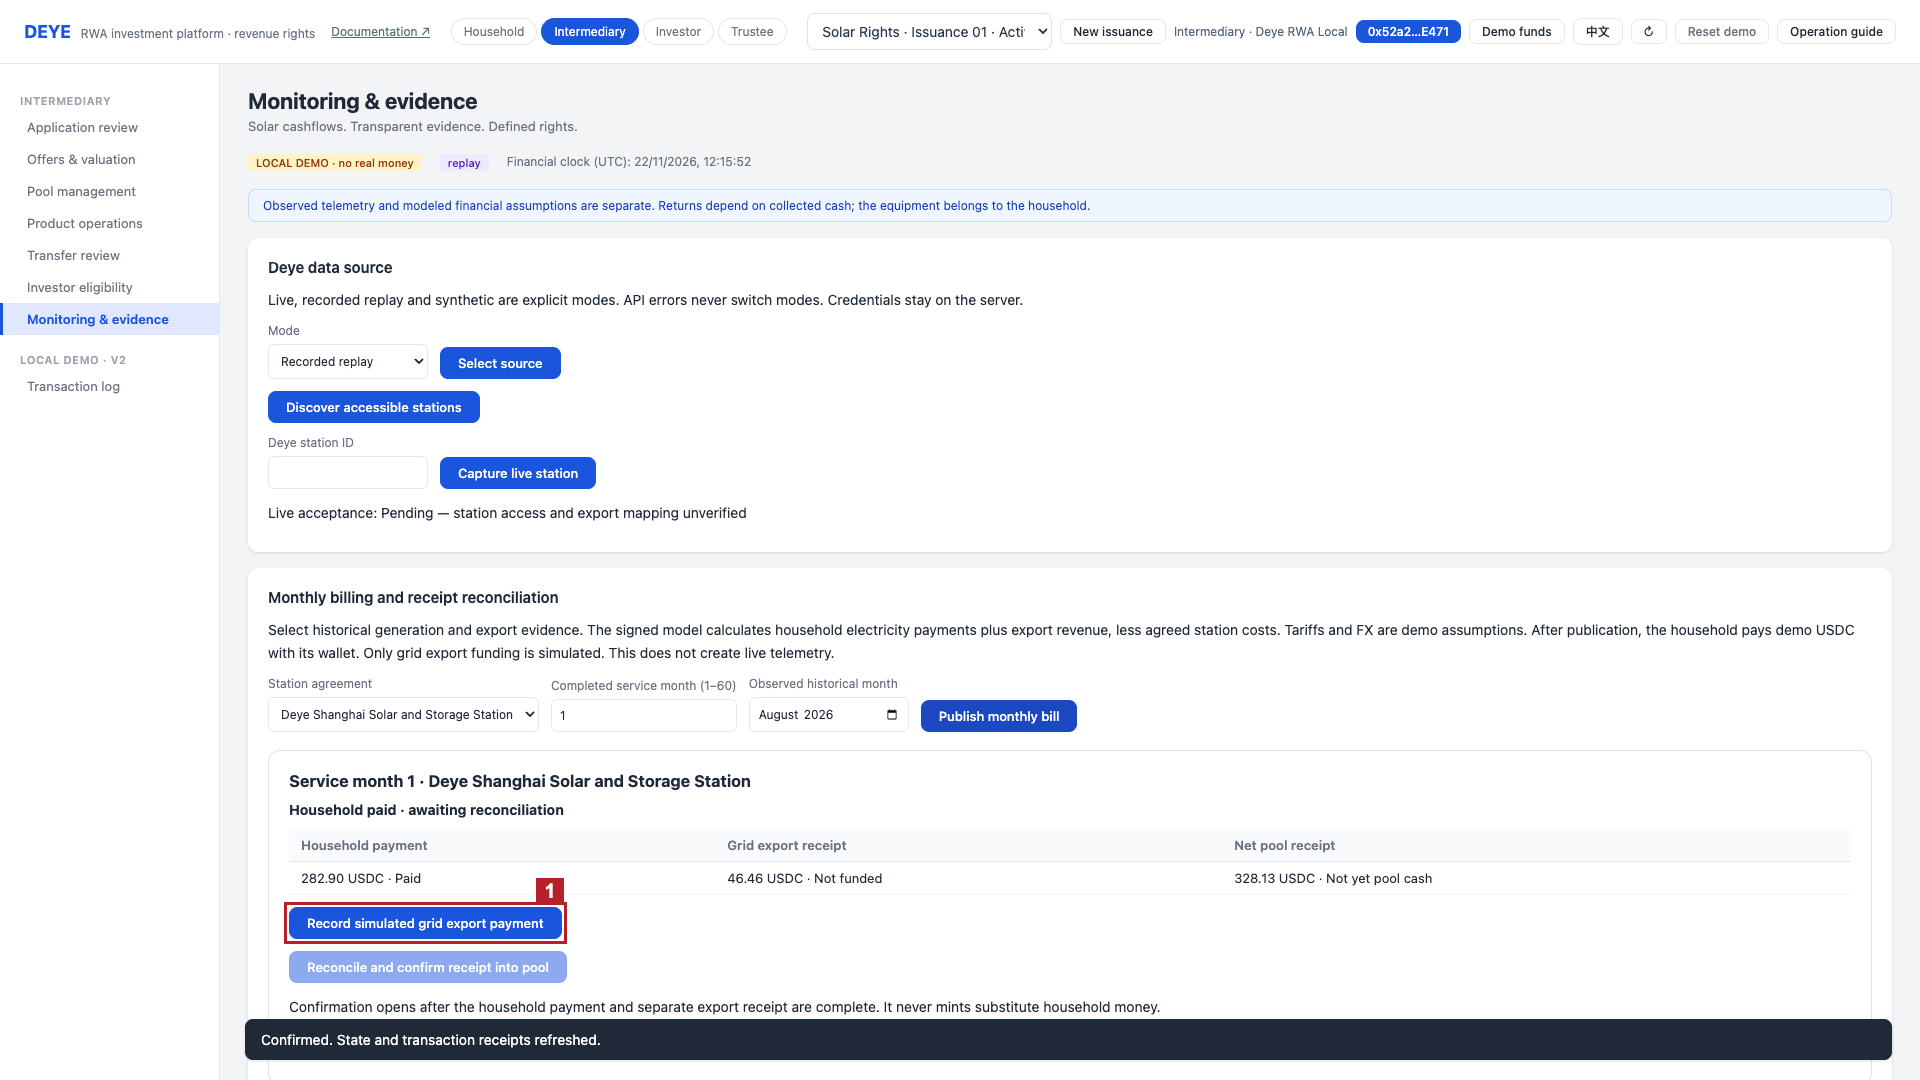
\includegraphics[width=\linewidth,height=.56\textheight,keepaspectratio]{assets/E3a.en-context.png}\par Marker 1 identifies the control or information to inspect for this step. Amounts and dates refer to the isolated demonstration.\end{center}
\begin{center}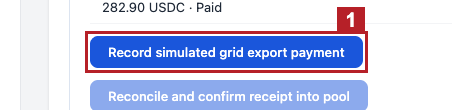
\includegraphics[width=.7\linewidth,height=1.55cm,keepaspectratio]{assets/E3a.en-detail.png}\end{center}
\end{landscape}
\clearpage\begin{landscape}
\subsection{E3b Reconcile and confirm receipt into the pool}
\label{step:E3b}
This step is performed by Intermediary. Inspect the household payment, export receipt, station expense and net amount on the same invoice. Use marker 1 to reconcile and confirm receipt into the pool, then confirm the intermediary wallet transaction.

After this step, the billing contract pays agreed station expenses once and transfers assigned net proceeds to the vault. The receivable clears once. Completed historical collections are not charged again. Continue with monthly fees and valuation approval.

\begin{center}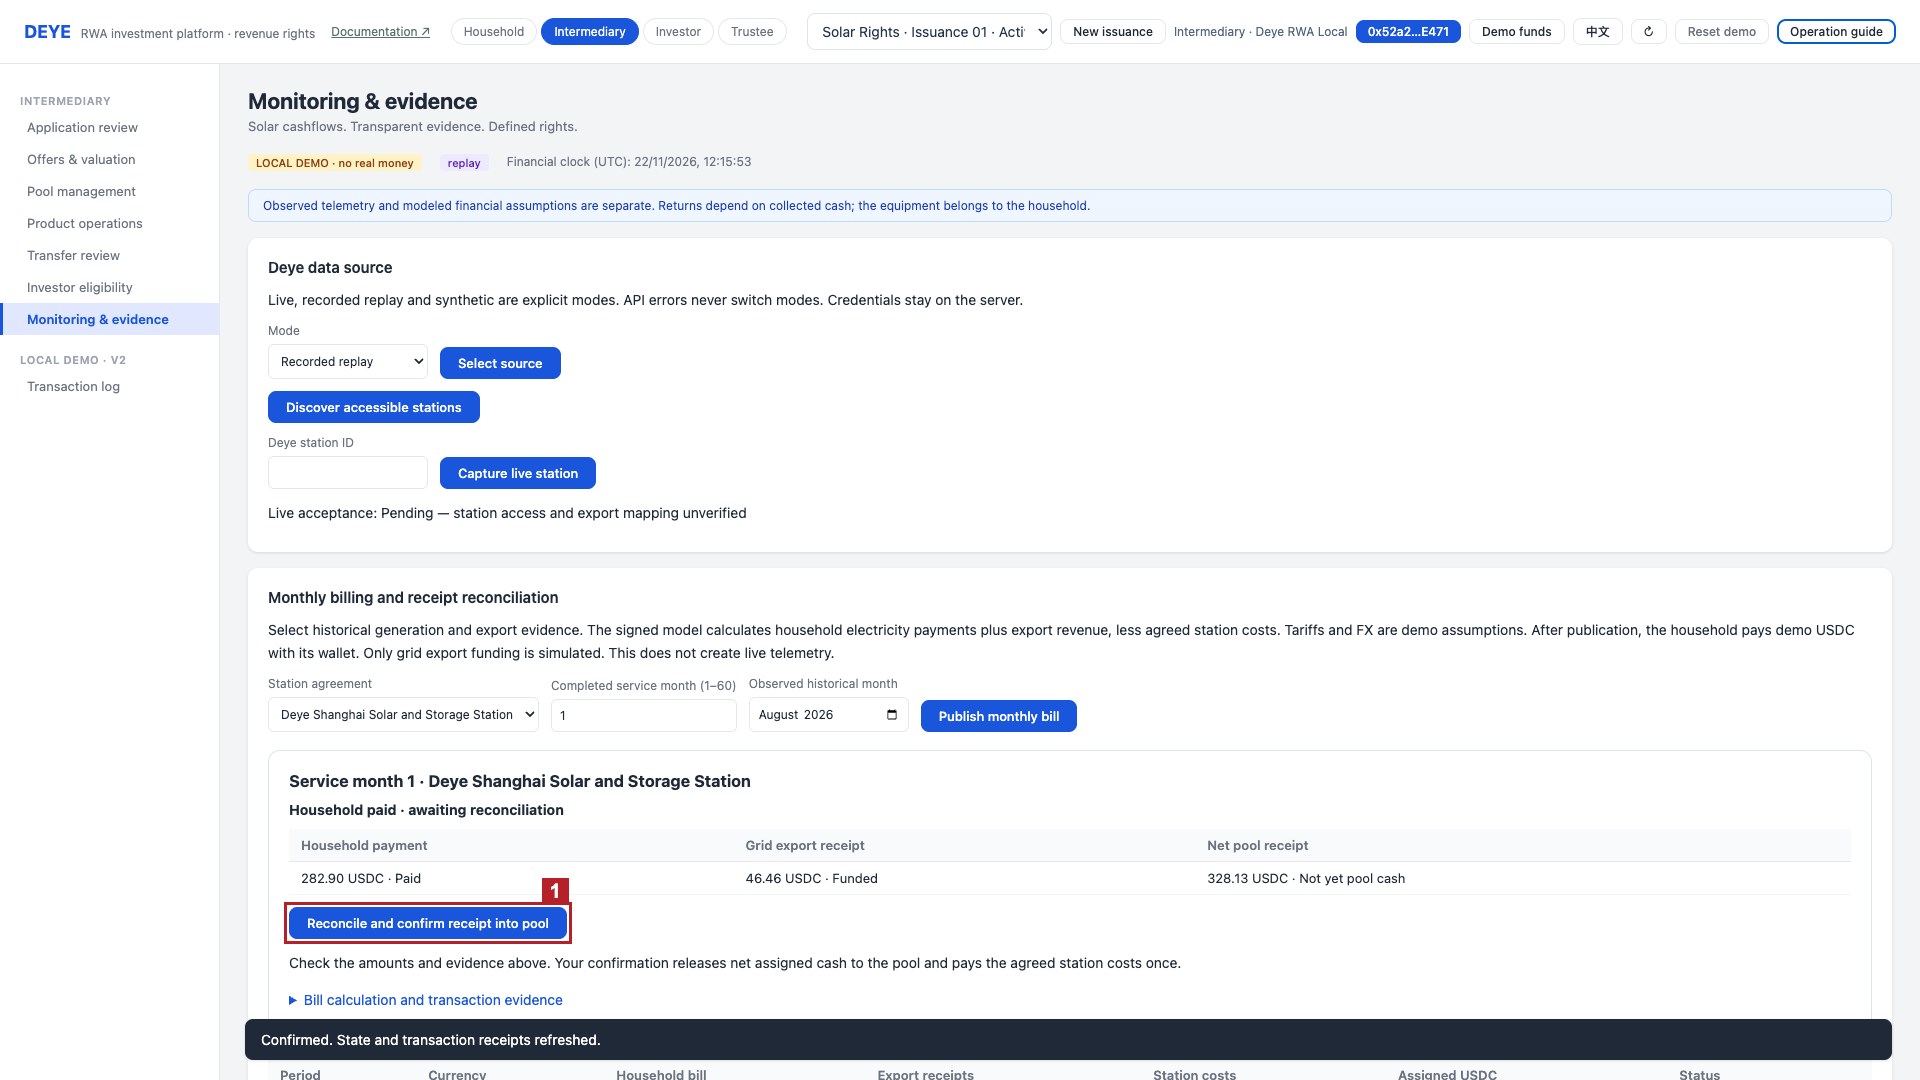
\includegraphics[width=\linewidth,height=.56\textheight,keepaspectratio]{assets/E3b.en-context.png}\par Marker 1 identifies the control or information to inspect for this step. Amounts and dates refer to the isolated demonstration.\end{center}
\begin{center}
\includegraphics[width=.7\linewidth,height=1.55cm,keepaspectratio]{assets/E3b.en-detail.png}\end{center}
\end{landscape}
\clearpage\begin{landscape}
\subsection{E4 Monthly pool expense accrual}
\label{step:E4}
This step is performed by Intermediary. Check the fee cutoff and the approved opening NAV for this fee period. If the basis is missing, follow the guide to prepare a report and obtain trustee approval. Accrue the monthly annual-fee fraction and mandatory pool costs once. Accrual records liabilities rather than another immediate cash payment.

After this step, prepare the post-accounting valuation for trustee approval.

\begin{center}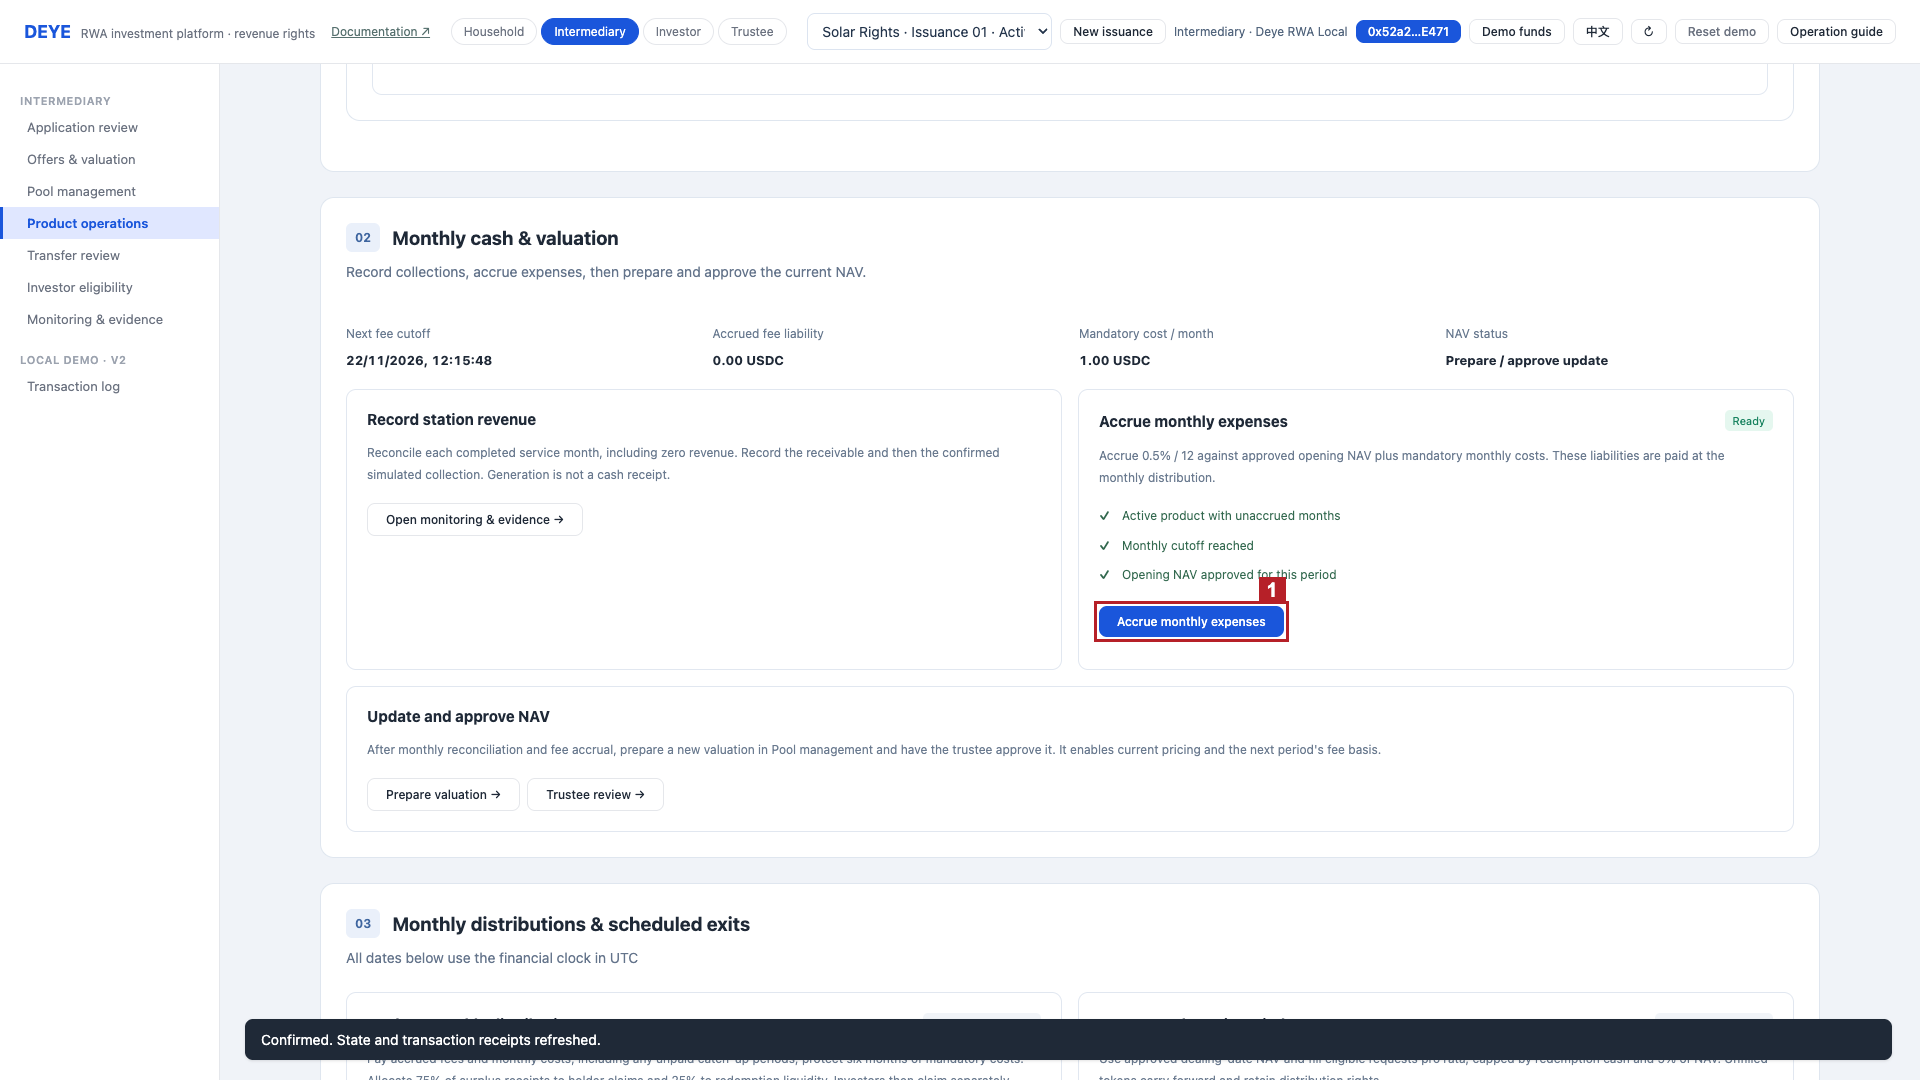
\includegraphics[width=\linewidth,height=.56\textheight,keepaspectratio]{assets/E4.en-context.png}\par Marker 1 identifies the control or information to inspect for this step. Amounts and dates refer to the isolated demonstration.\end{center}
\begin{center}
\includegraphics[width=.7\linewidth,height=1.55cm,keepaspectratio]{assets/E4.en-detail.png}\end{center}
\end{landscape}
\clearpage\begin{landscape}
\subsection{E5 Monthly valuation approval}
\label{step:E5}
This step is performed by Intermediary, followed by trustee. Prepare a report after receipts and fee accrual are reconciled. The trustee must check the current report and approve its anchor transaction. An older fully paid distribution must not replace this pending approval task. Reprepare a report whose inputs or validity have changed.

After this step, return to the intermediary for the monthly distribution declaration.

\begin{center}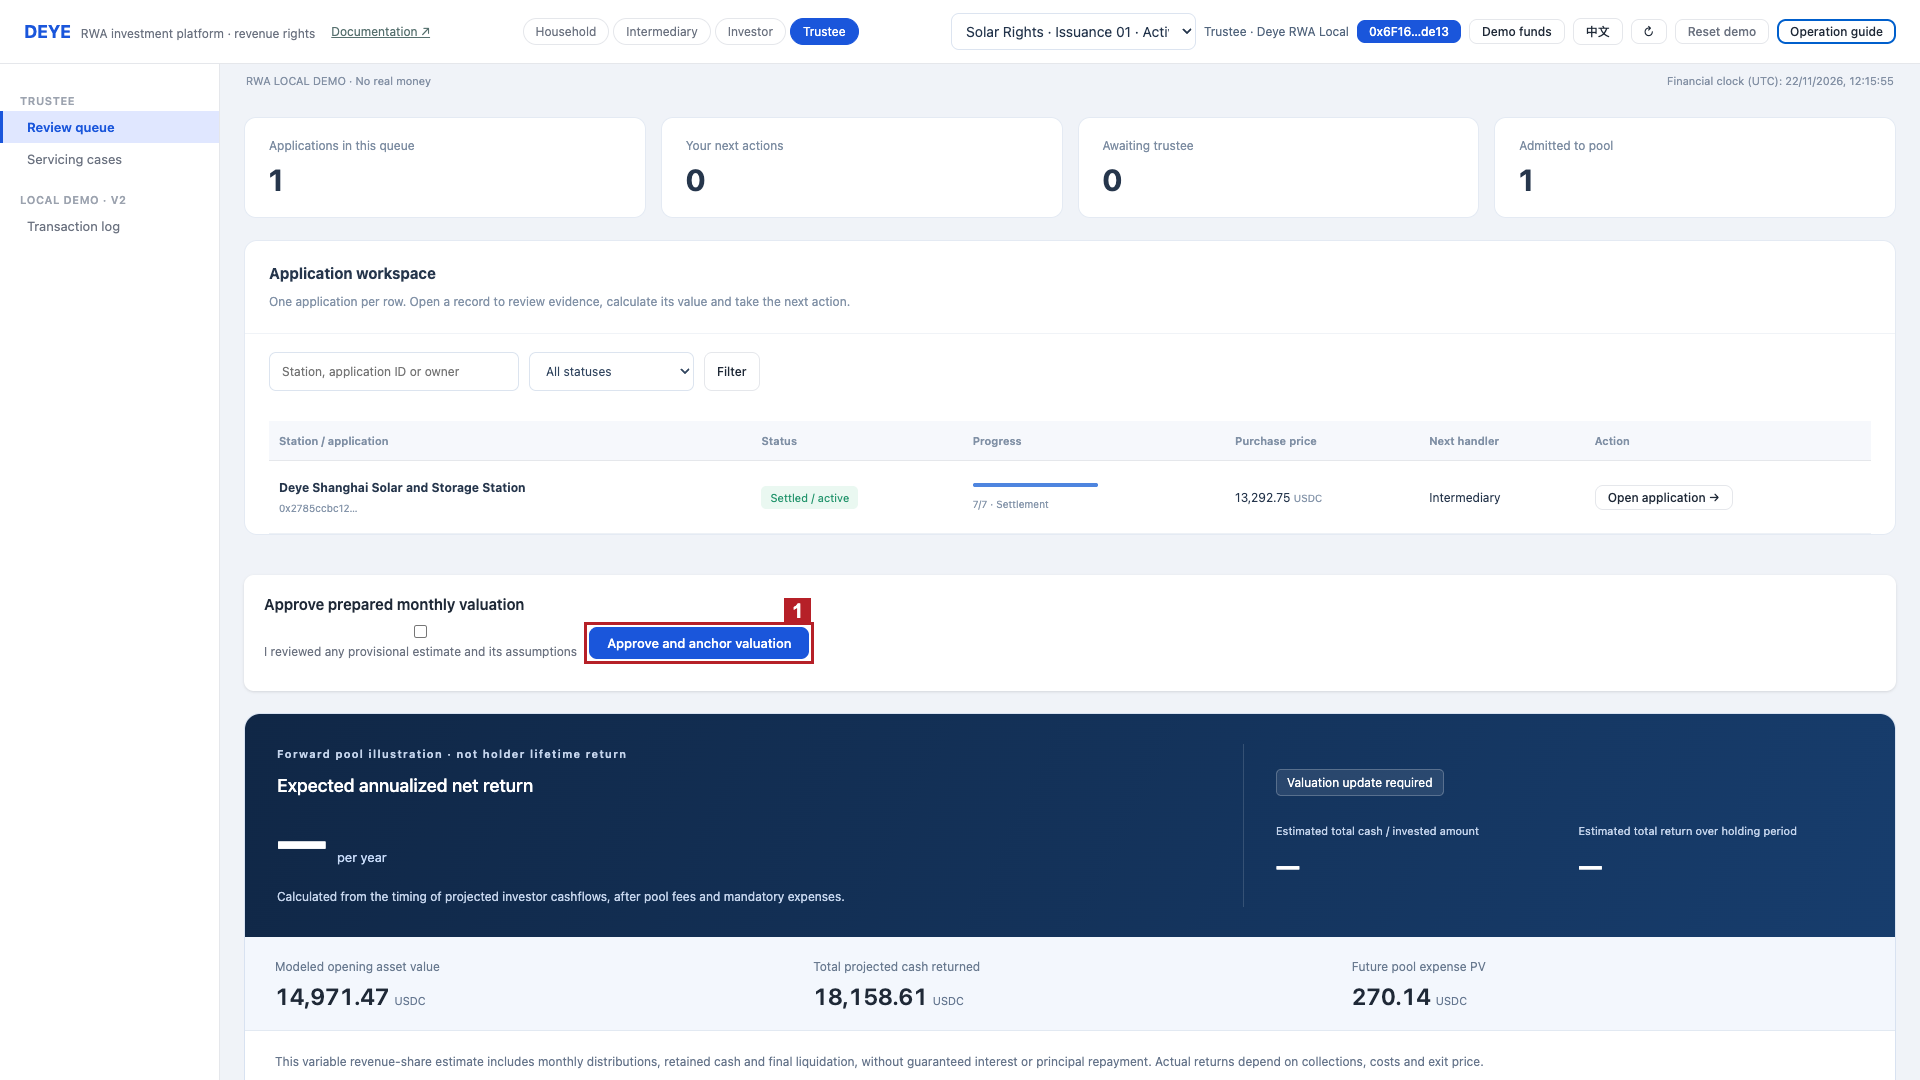
\includegraphics[width=\linewidth,height=.56\textheight,keepaspectratio]{assets/E5.en-context.png}\par Marker 1 identifies the control or information to inspect for this step. Amounts and dates refer to the isolated demonstration.\end{center}
\begin{center}
\includegraphics[width=.7\linewidth,height=1.55cm,keepaspectratio]{assets/E5.en-detail.png}\end{center}
\end{landscape}
\clearpage\begin{landscape}
\subsection{E6 Monthly distribution declaration}
\label{step:E6}
This step is performed by Intermediary. After the current report is approved, declare the due monthly distribution. The contract pays applicable accrued expenses, restores six months of mandatory-cost reserve and allocates eligible remaining receipts 75\% to distribution and 25\% to redemption liquidity. The initial retained cash is not treated as distributable revenue.

After this step, follow the explicit handoff to the investor to inspect and claim this new distribution.

\begin{center}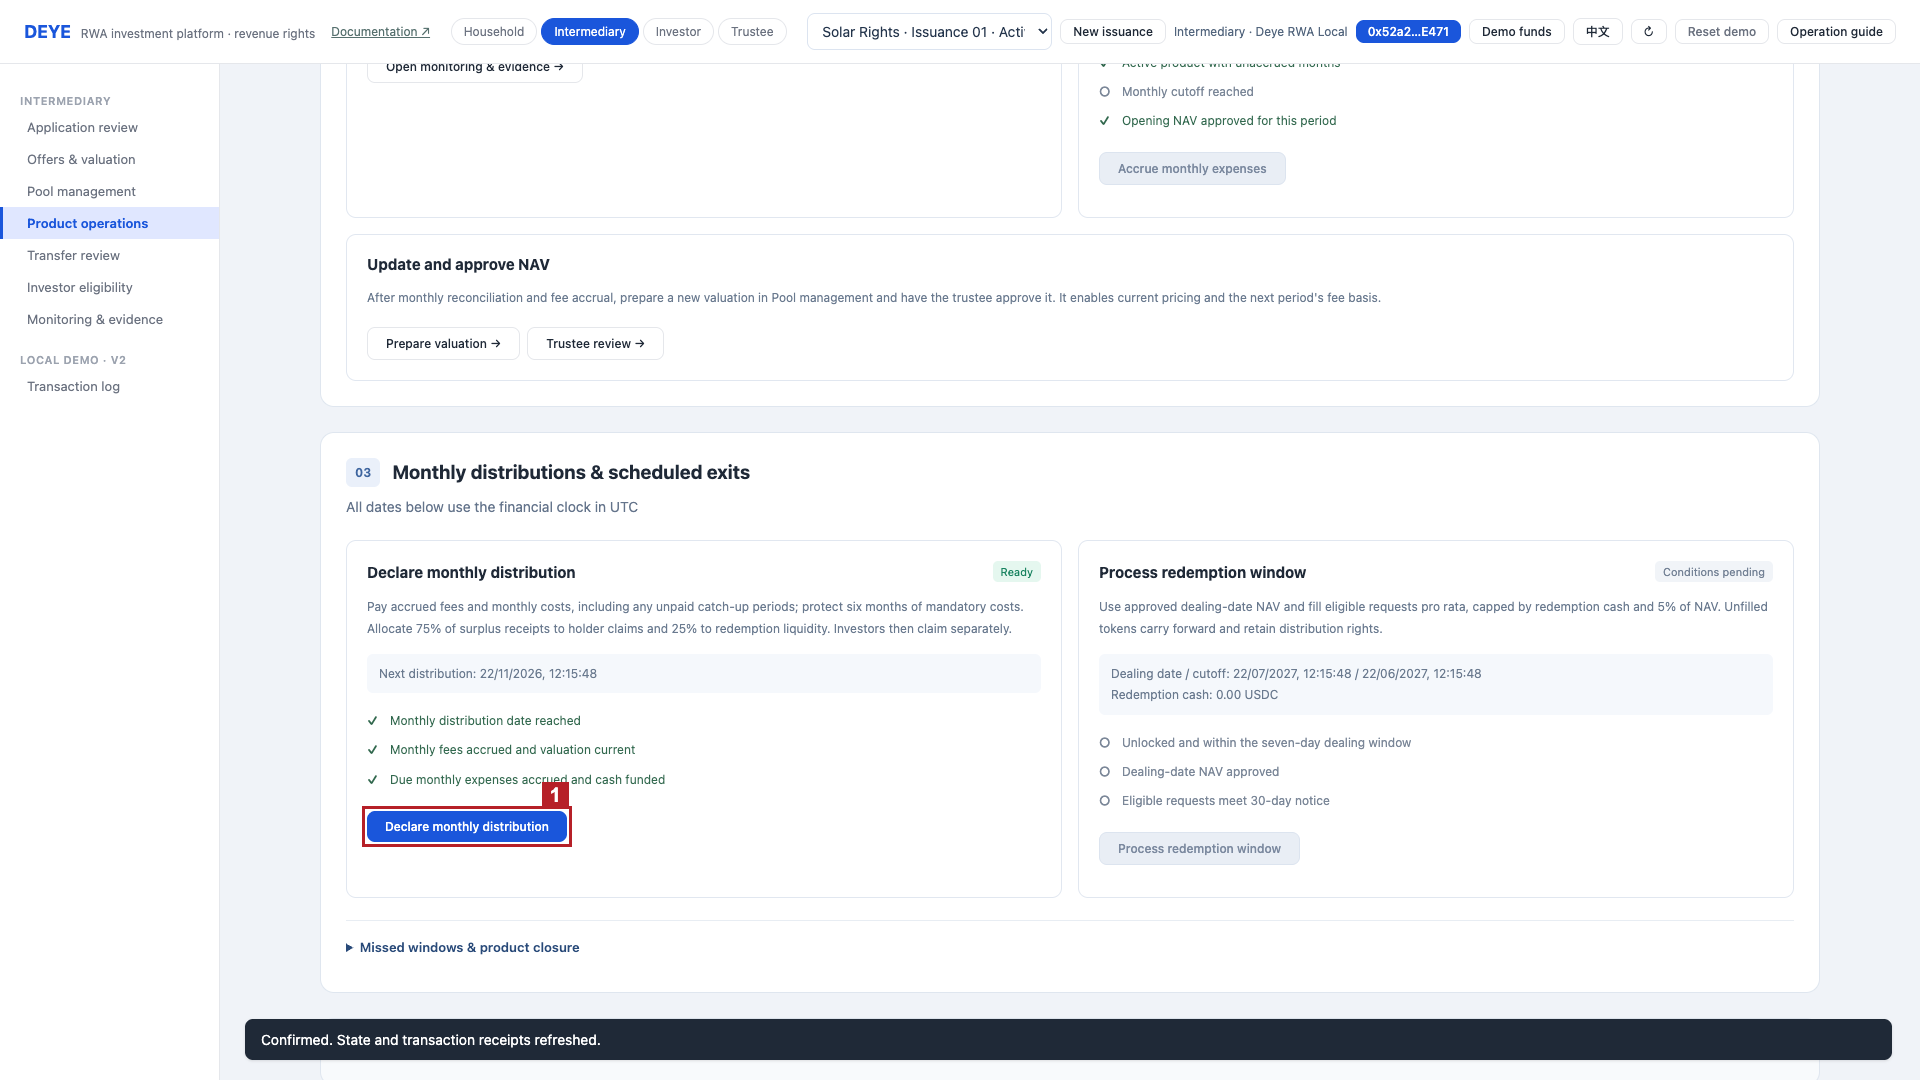
\includegraphics[width=\linewidth,height=.56\textheight,keepaspectratio]{assets/E6.en-context.png}\par Marker 1 identifies the control or information to inspect for this step. Amounts and dates refer to the isolated demonstration.\end{center}
\begin{center}
\includegraphics[width=.7\linewidth,height=1.55cm,keepaspectratio]{assets/E6.en-detail.png}\end{center}
\end{landscape}
\clearpage\begin{landscape}
\subsection{E7 Distribution claim}
\label{step:E7}
This step is performed by Investor. Open My holdings and locate the newly declared distribution identifier. Check the positive claimable amount, confirm Claim in Rabby and compare the wallet balance before and after confirmation. A paid record remains historical and must not continue to appear as payable.

After this step, staff can reconcile the next month after the claim or explicitly defer investor viewing.

\begin{center}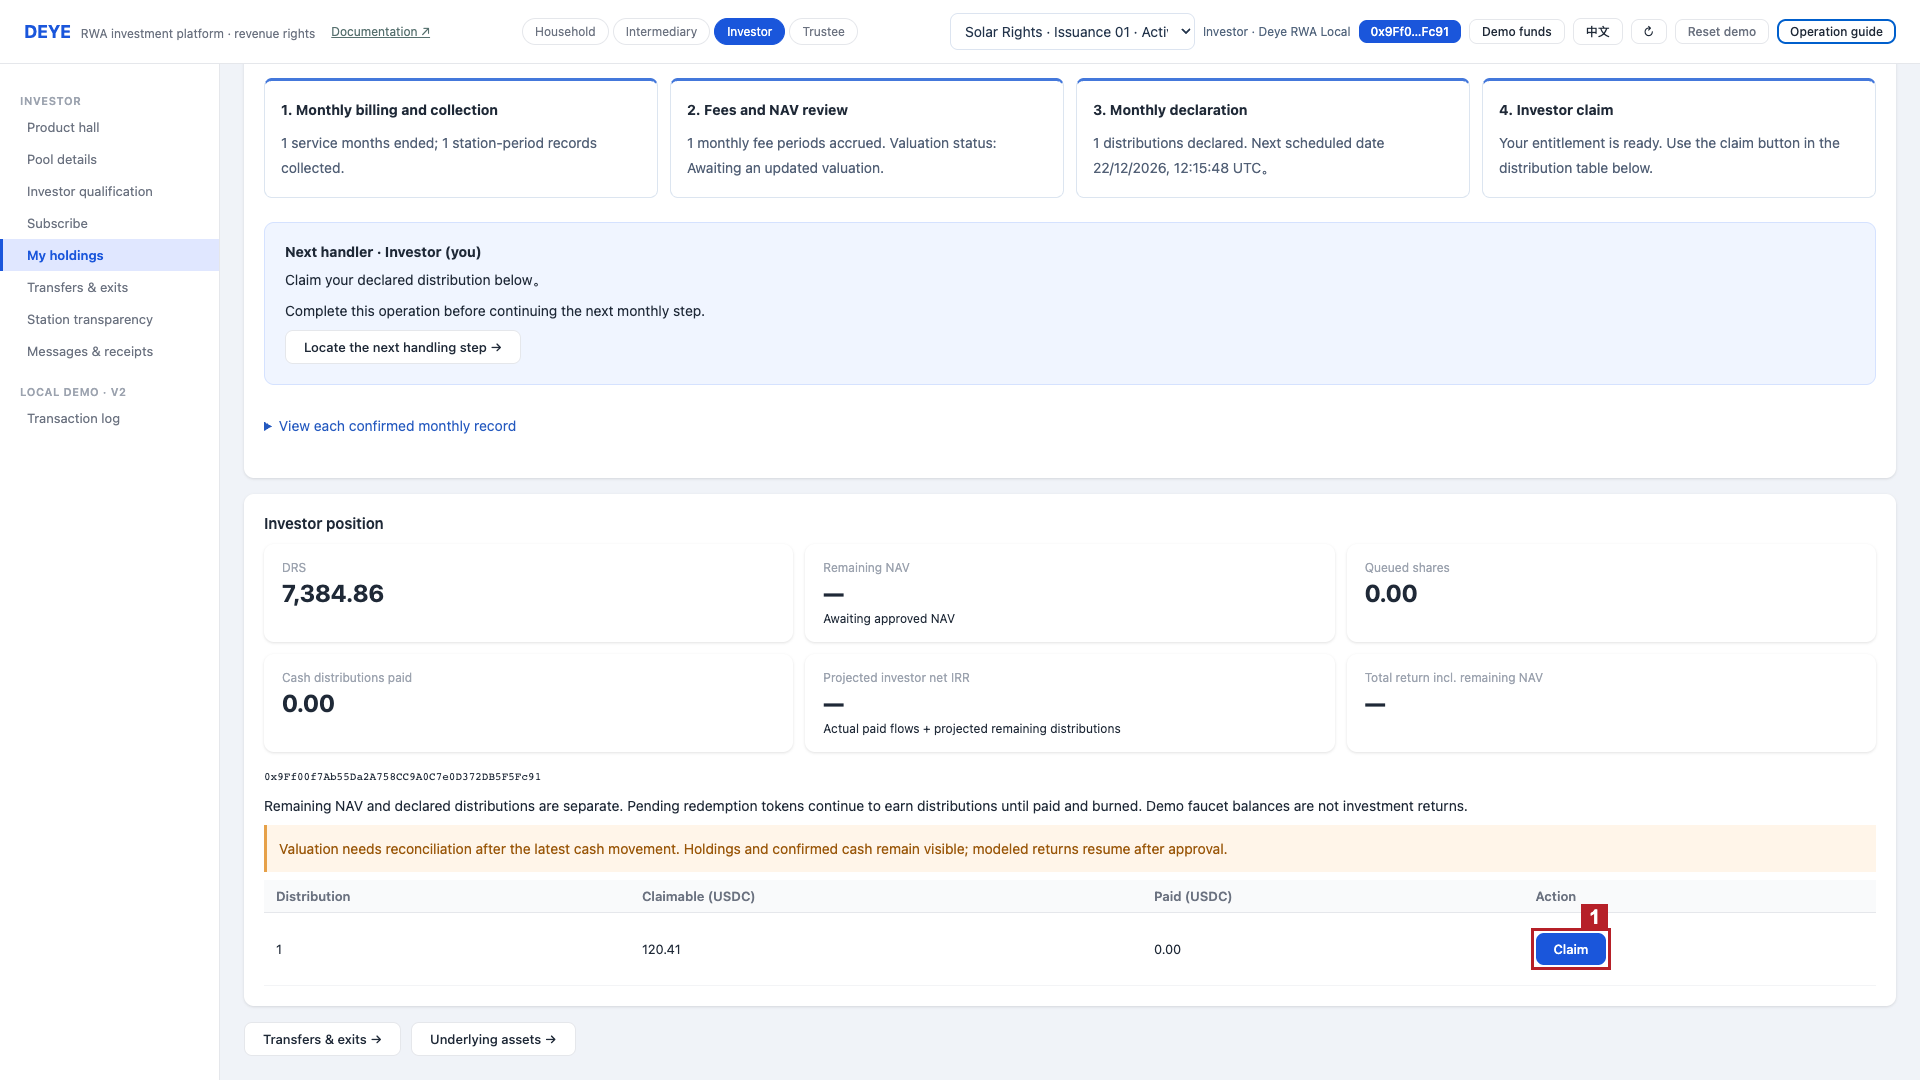
\includegraphics[width=\linewidth,height=.56\textheight,keepaspectratio]{assets/E7.en-context.png}\par Marker 1 identifies the control or information to inspect for this step. Amounts and dates refer to the isolated demonstration.\end{center}
\begin{center}
\includegraphics[width=.7\linewidth,height=1.55cm,keepaspectratio]{assets/E7.en-detail.png}\end{center}
\end{landscape}
\clearpage\begin{landscape}
\section{Peer transfers and quarterly redemption}
\subsection{F1 Peer transfer proposal}
\label{step:F1}
This step is performed by Investor A as seller. After the six-month lock, enter the eligible buyer, share quantity and negotiated USDC total in Transfers and exits. Submit the exact terms and inspect the NAV comparison. A proposal does not itself transfer shares or collect payment.

After this step, investor B accepts these terms and authorizes payment.

\begin{center}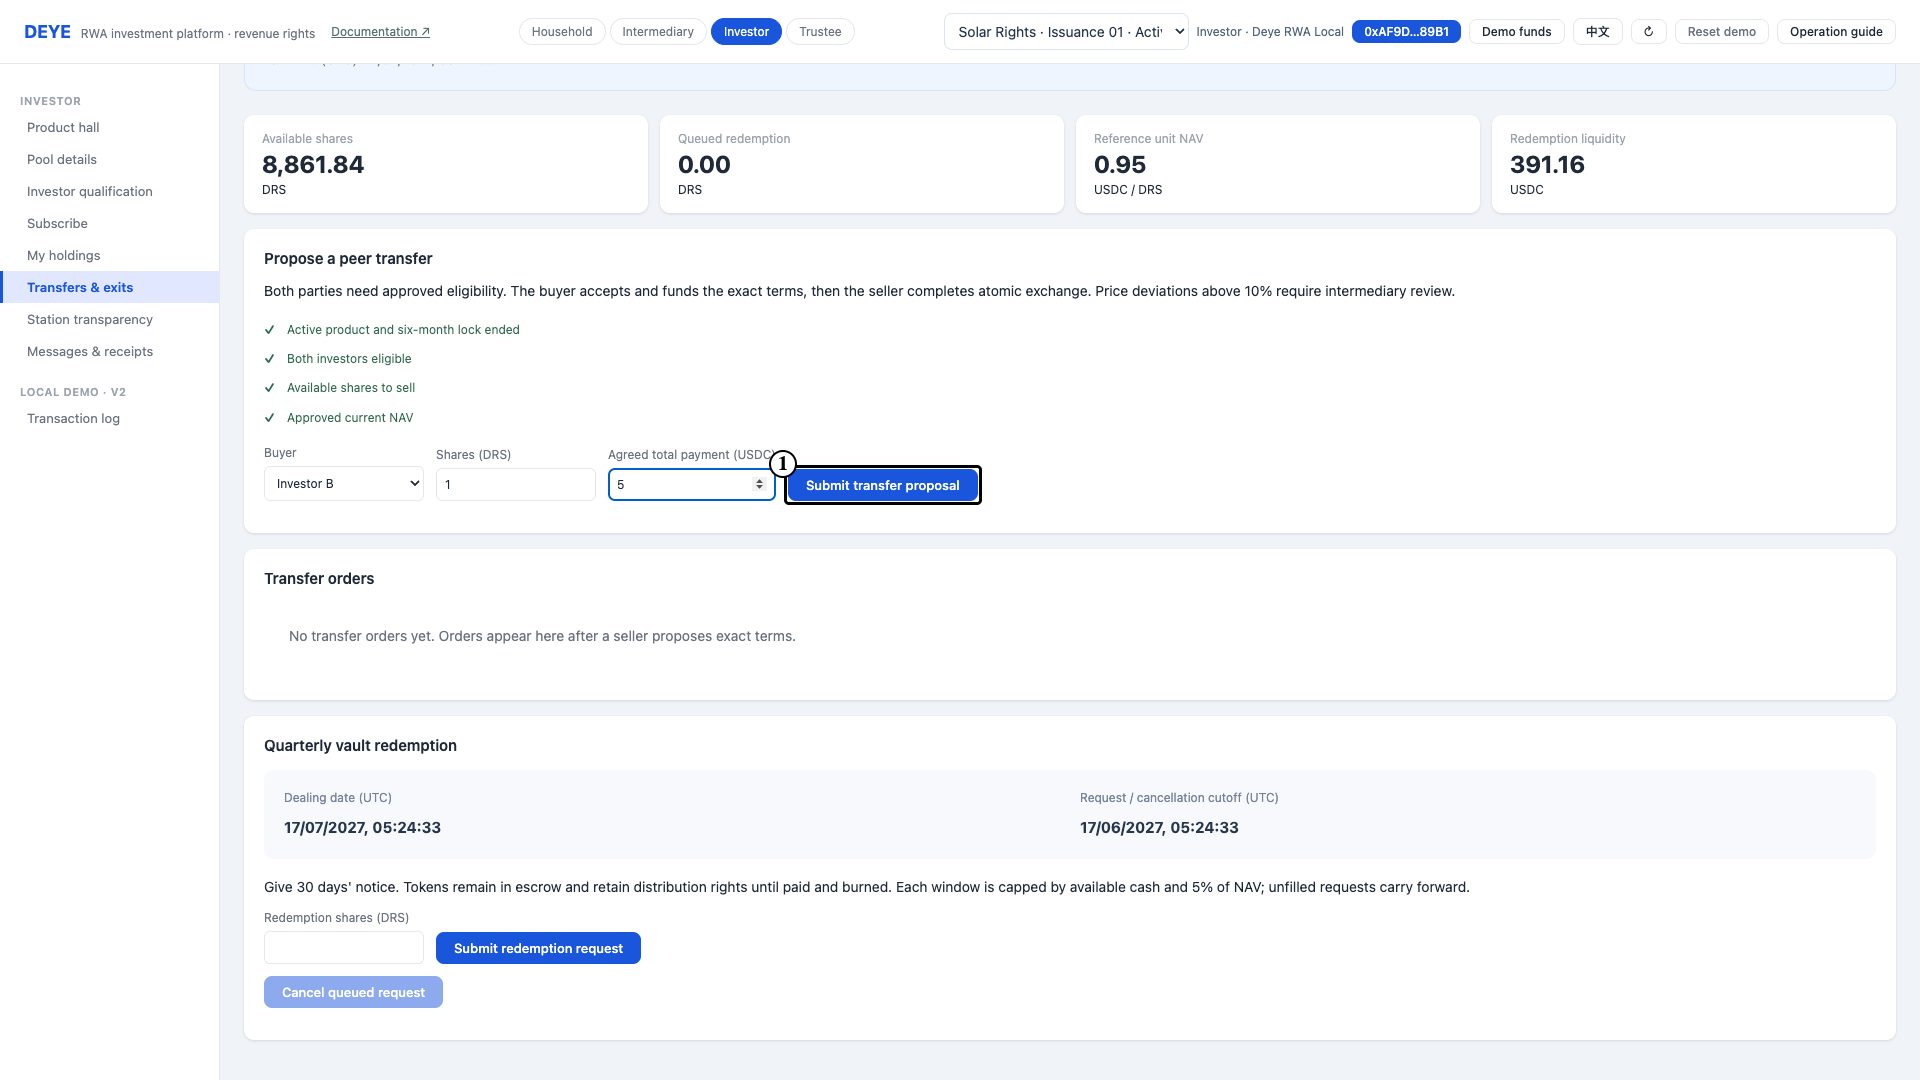
\includegraphics[width=\linewidth,height=.44\textheight,keepaspectratio]{assets/F1.en-context.png}\par Marker 1 identifies the control or information to inspect for this step. Amounts and dates refer to the isolated demonstration.\end{center}
\begin{center}
\includegraphics[width=.7\linewidth,height=1.55cm,keepaspectratio]{assets/F1.en-detail.png}\end{center}
\end{landscape}
\clearpage\begin{landscape}
\subsection{F2 Buyer consent and payment approval}
\label{step:F2}
This step is performed by Investor B. Open the proposed transfer and verify the seller, shares and total consideration. Complete the required USDC approval and buyer-consent transactions in the indicated order. Consent is bound to these exact terms and cannot be supplied by the seller.

After this step, obtain intermediary price review if the deviation exceeds 10\%.

\begin{center}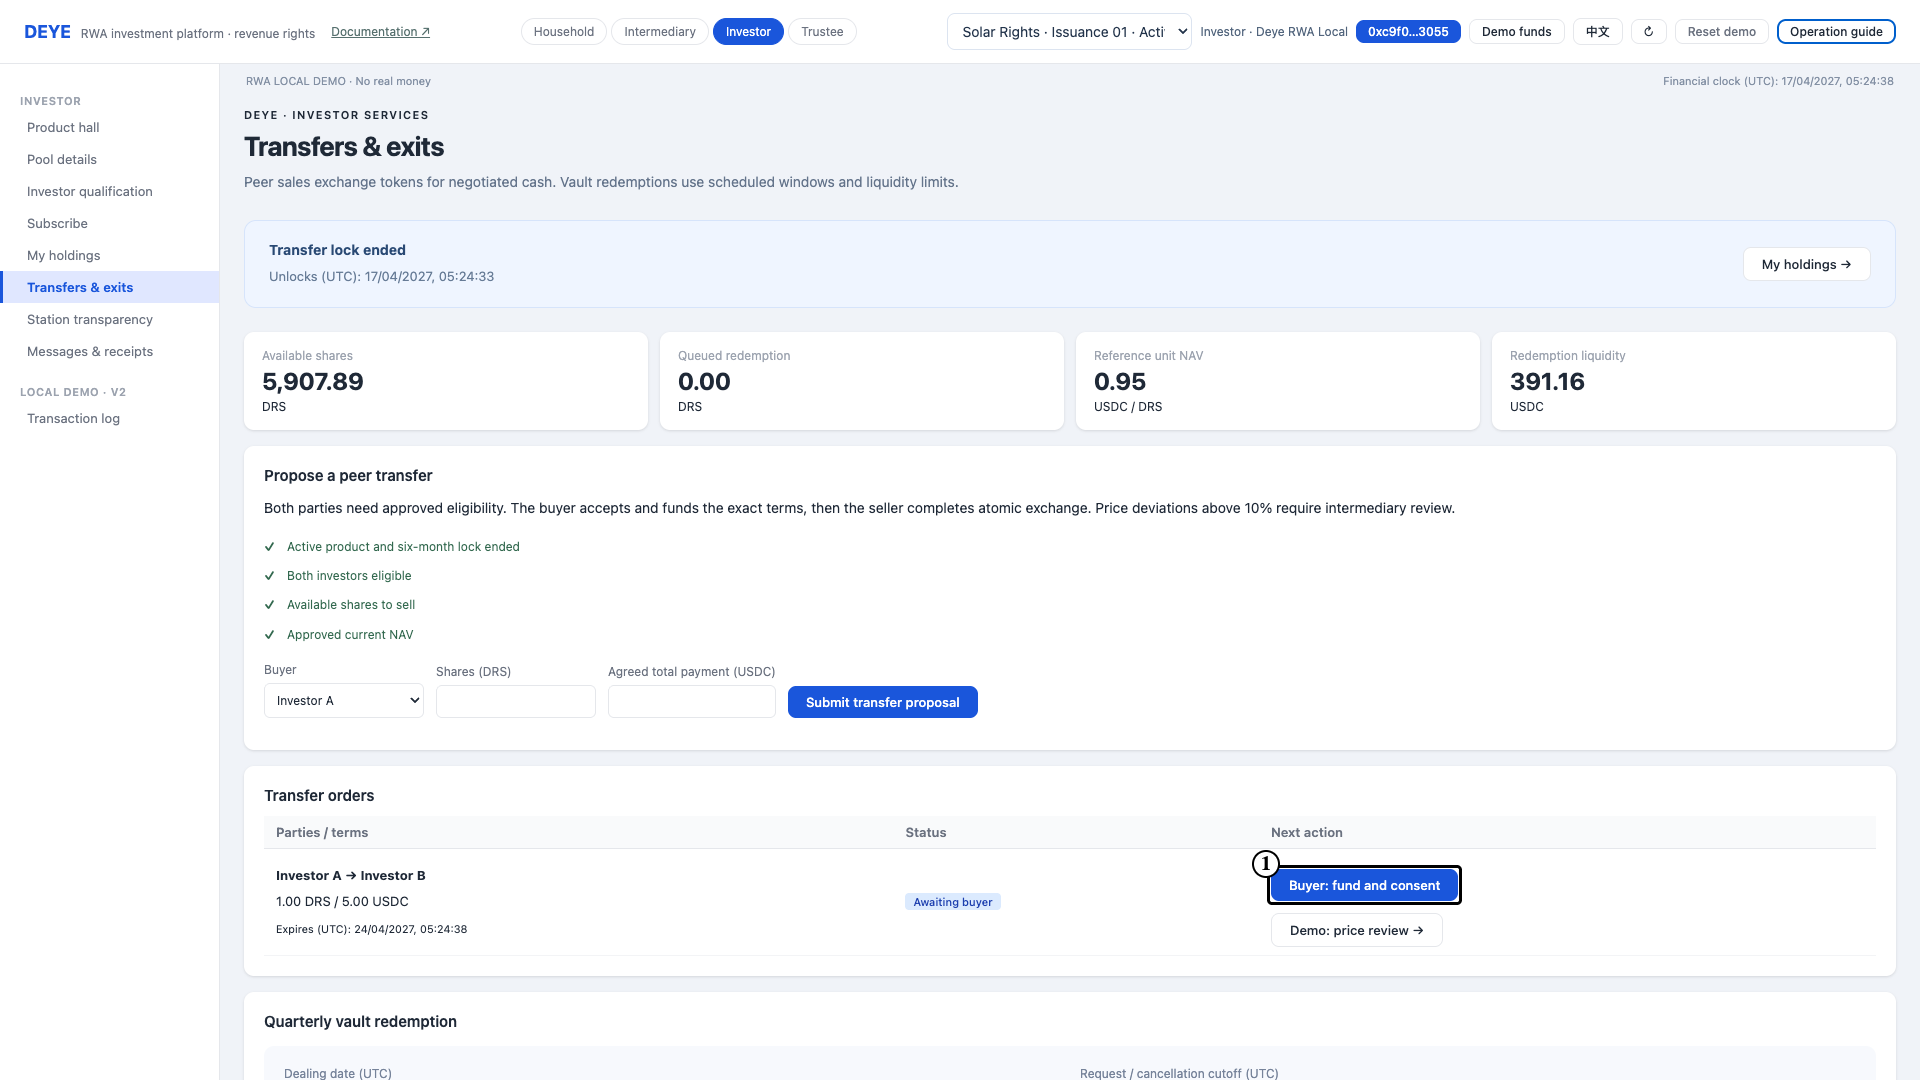
\includegraphics[width=\linewidth,height=.56\textheight,keepaspectratio]{assets/F2.en-context.png}\par Marker 1 identifies the control or information to inspect for this step. Amounts and dates refer to the isolated demonstration.\end{center}
\begin{center}
\includegraphics[width=.7\linewidth,height=1.55cm,keepaspectratio]{assets/F2.en-detail.png}\end{center}
\end{landscape}
\clearpage\begin{landscape}
\subsection{F3 Transfer price review}
\label{step:F3}
This step is performed by Intermediary. Open Transfer review and compare the negotiated price with the approved NAV reference. Record the required approval for a deviation above 10\%. Review does not guarantee the price or complete either transfer leg.

After this step, the seller completes atomic settlement.

\begin{center}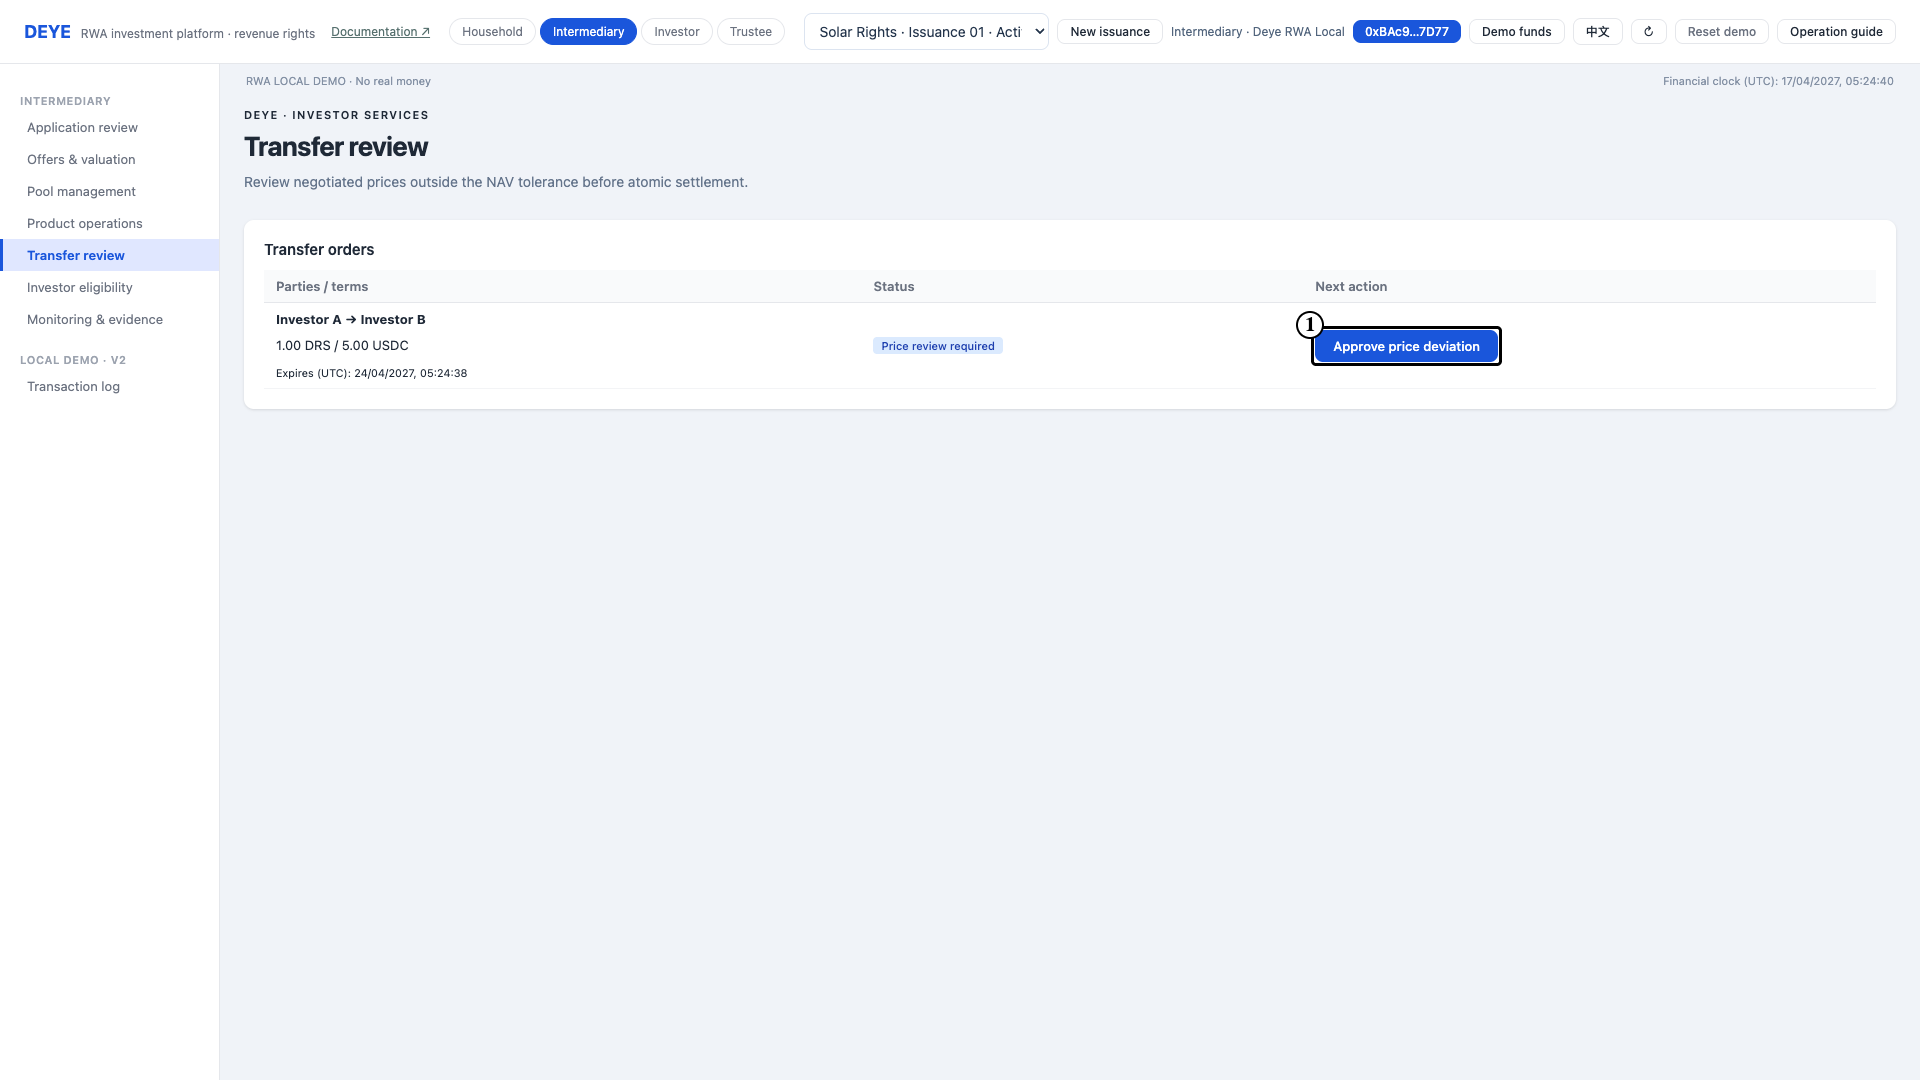
\includegraphics[width=\linewidth,height=.56\textheight,keepaspectratio]{assets/F3.en-context.png}\par Marker 1 identifies the control or information to inspect for this step. Amounts and dates refer to the isolated demonstration.\end{center}
\begin{center}
\includegraphics[width=.7\linewidth,height=1.55cm,keepaspectratio]{assets/F3.en-detail.png}\end{center}
\end{landscape}
\clearpage\begin{landscape}
\subsection{F4 Atomic peer settlement}
\label{step:F4}
This step is performed by Investor A as seller. Check buyer consent, allowance, eligibility, lock and required review, then confirm settlement. A successful transaction transfers shares to the buyer and USDC to the seller together. Verify both token transfers in Blockscout.

After this step, both investors review their updated positions.

\begin{center}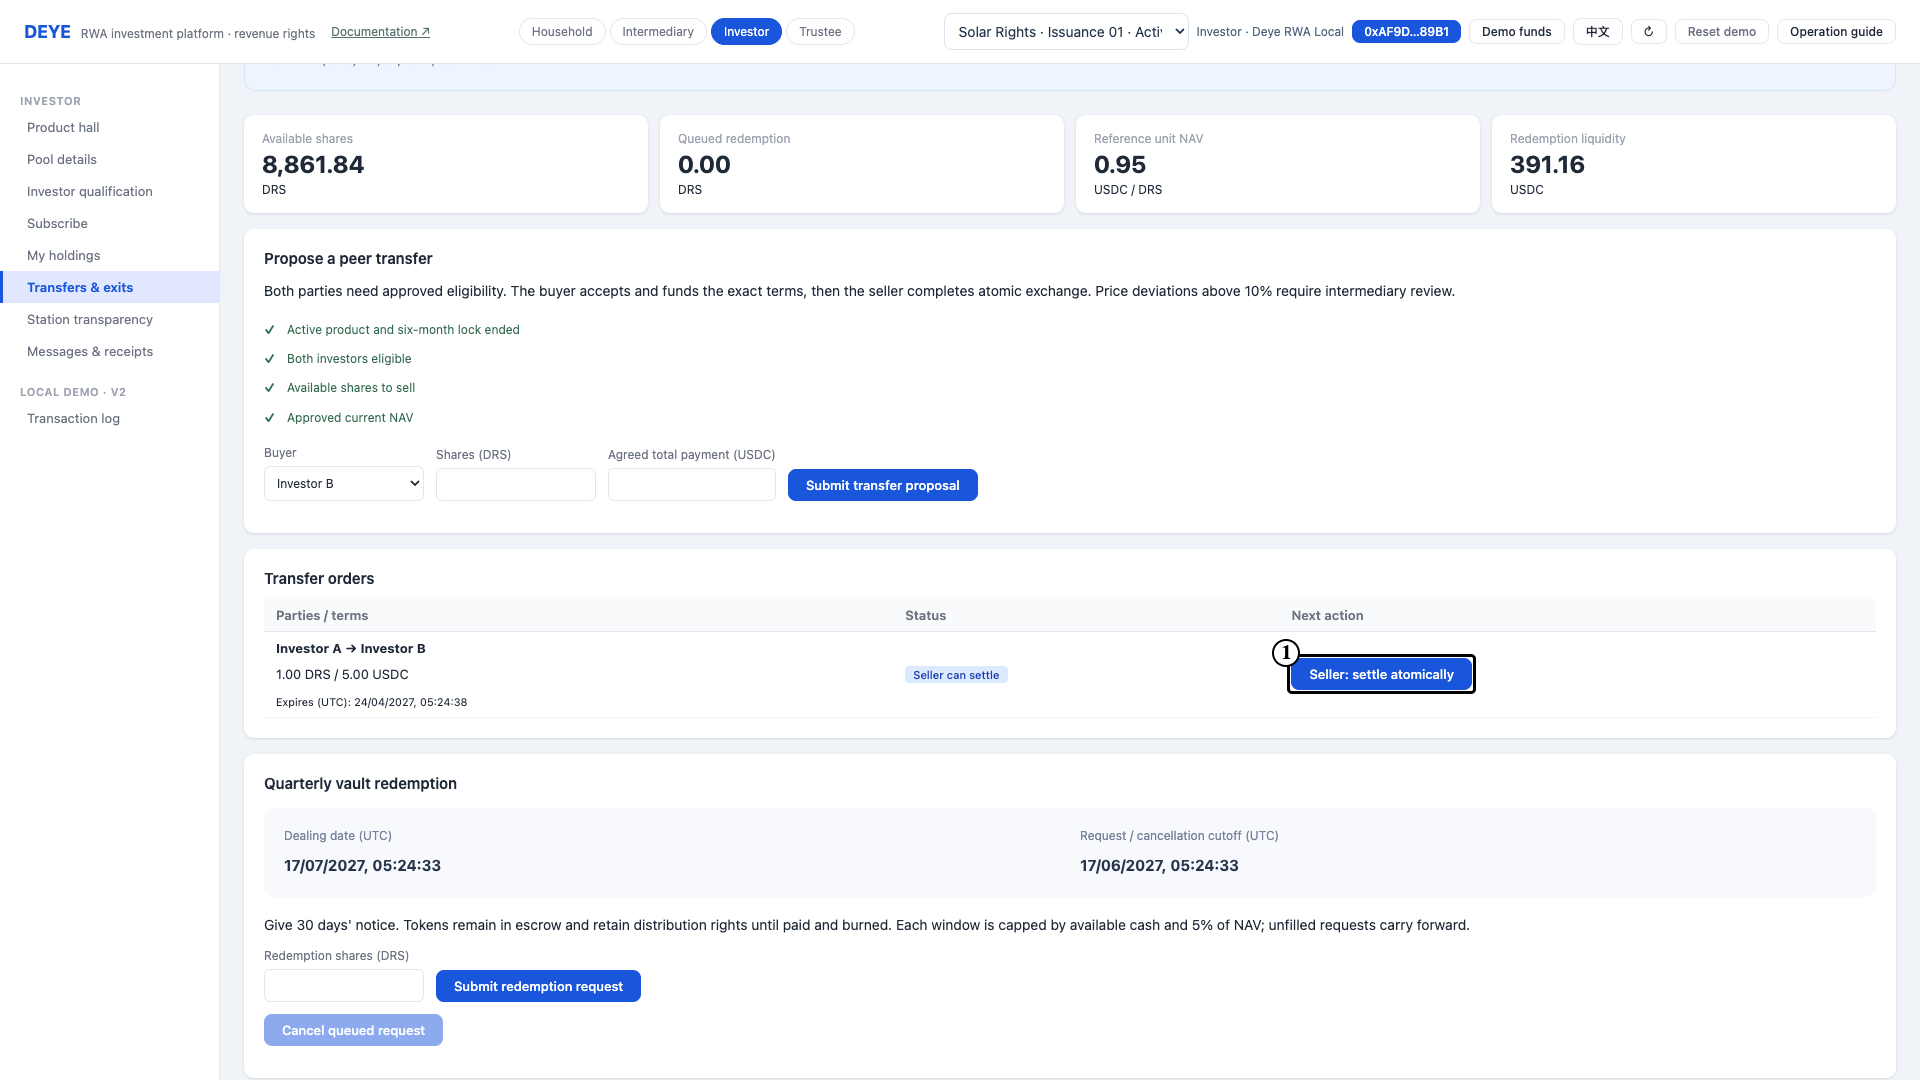
\includegraphics[width=\linewidth,height=.56\textheight,keepaspectratio]{assets/F4.en-context.png}\par Marker 1 identifies the control or information to inspect for this step. Amounts and dates refer to the isolated demonstration.\end{center}
\begin{center}
\includegraphics[width=.7\linewidth,height=1.55cm,keepaspectratio]{assets/F4.en-detail.png}\end{center}
\end{landscape}
\clearpage\begin{landscape}
\subsection{F5 Quarterly redemption request}
\label{step:F5}
This step is performed by Investor. Before the notice cutoff, enter the shares to redeem and confirm the request. The shares enter escrow and remain entitled to distributions until paid. The request is not an immediate cash redemption at today's reference NAV.

After this step, the intermediary processes an eligible quarterly dealing window after the lock.

\begin{center}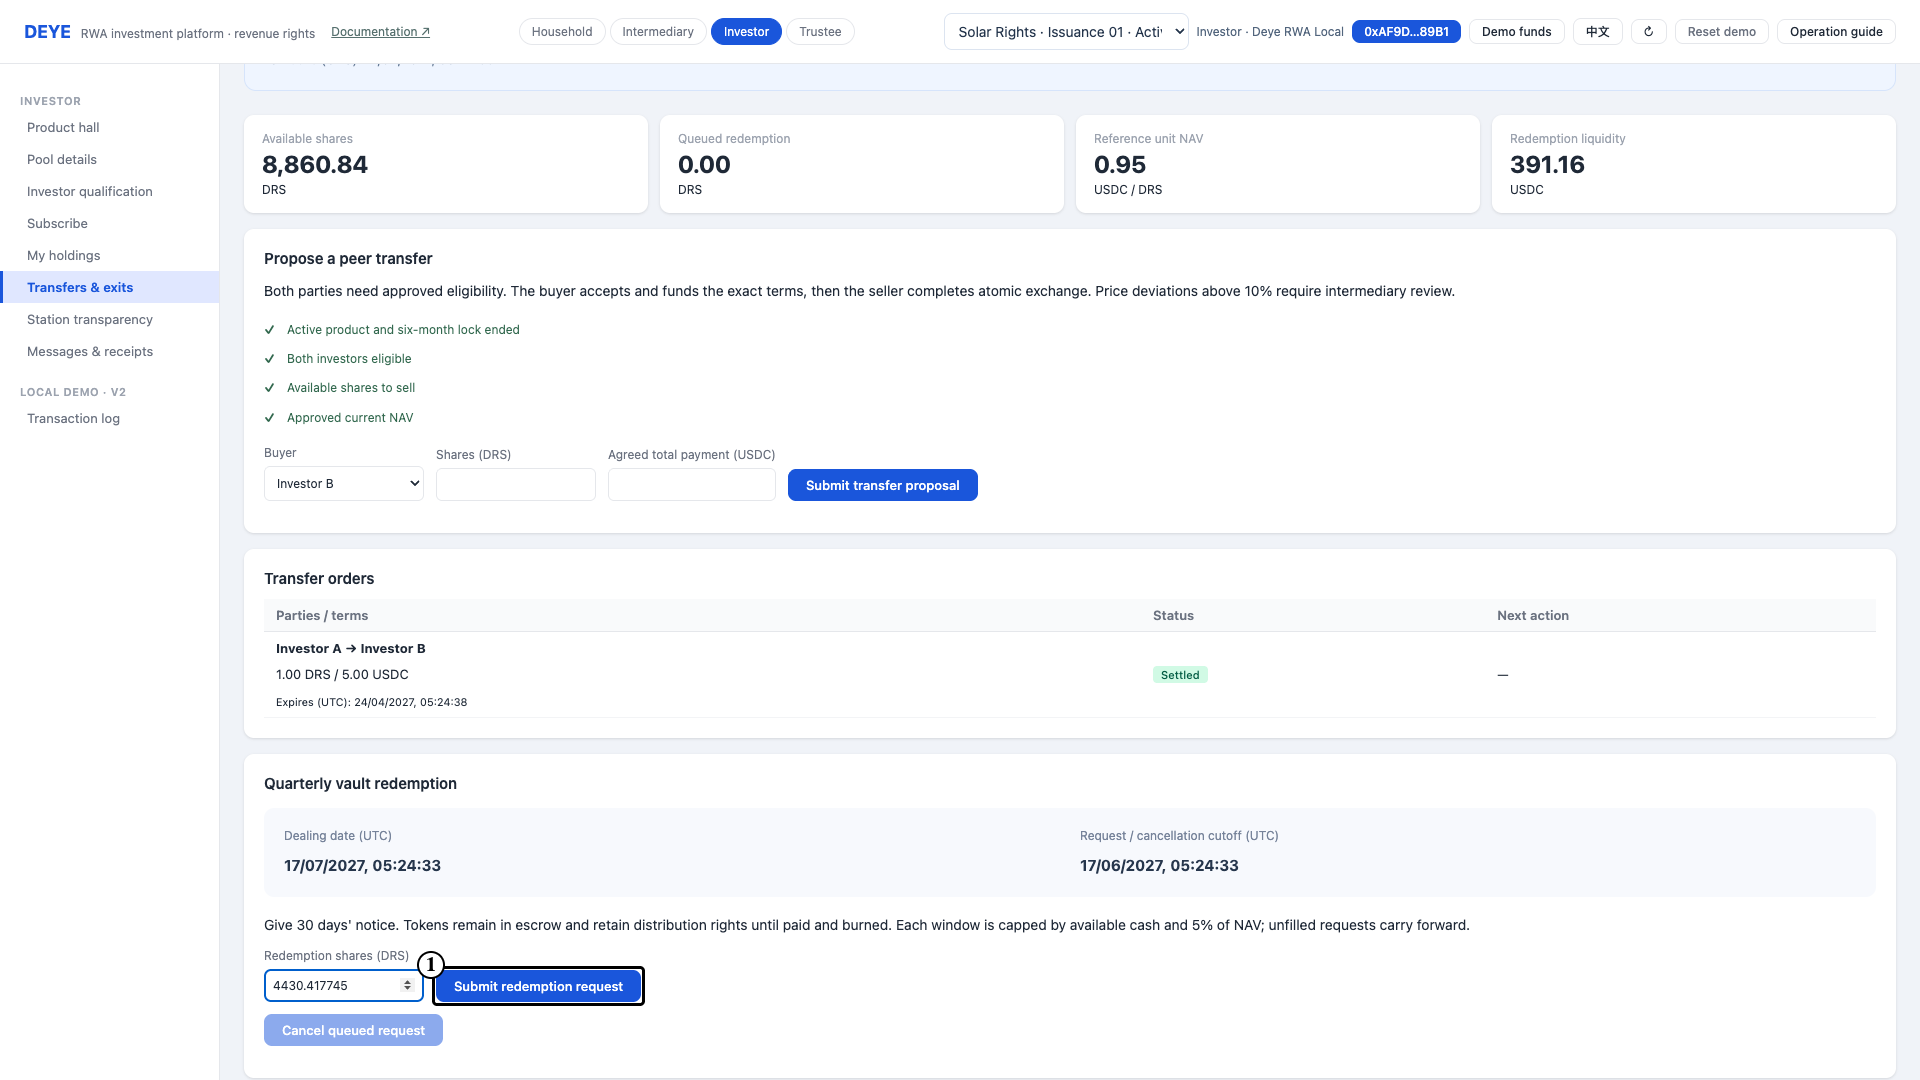
\includegraphics[width=\linewidth,height=.56\textheight,keepaspectratio]{assets/F5.en-context.png}\par Marker 1 identifies the control or information to inspect for this step. Amounts and dates refer to the isolated demonstration.\end{center}
\begin{center}
\includegraphics[width=.7\linewidth,height=1.55cm,keepaspectratio]{assets/F5.en-detail.png}\end{center}
\end{landscape}
\clearpage\begin{landscape}
\subsection{F6 Proportional redemption processing}
\label{step:F6}
This step is performed by Intermediary. At the eligible dealing date, reconcile and approve the dealing NAV before processing requests. Payment is capped by the lower of redemption liquidity and 5\% of pool NAV. The contract pays and burns only filled shares and carries the unfilled balance forward.

After this step, the investor checks payment, burned shares and the remaining escrow request.

\begin{center}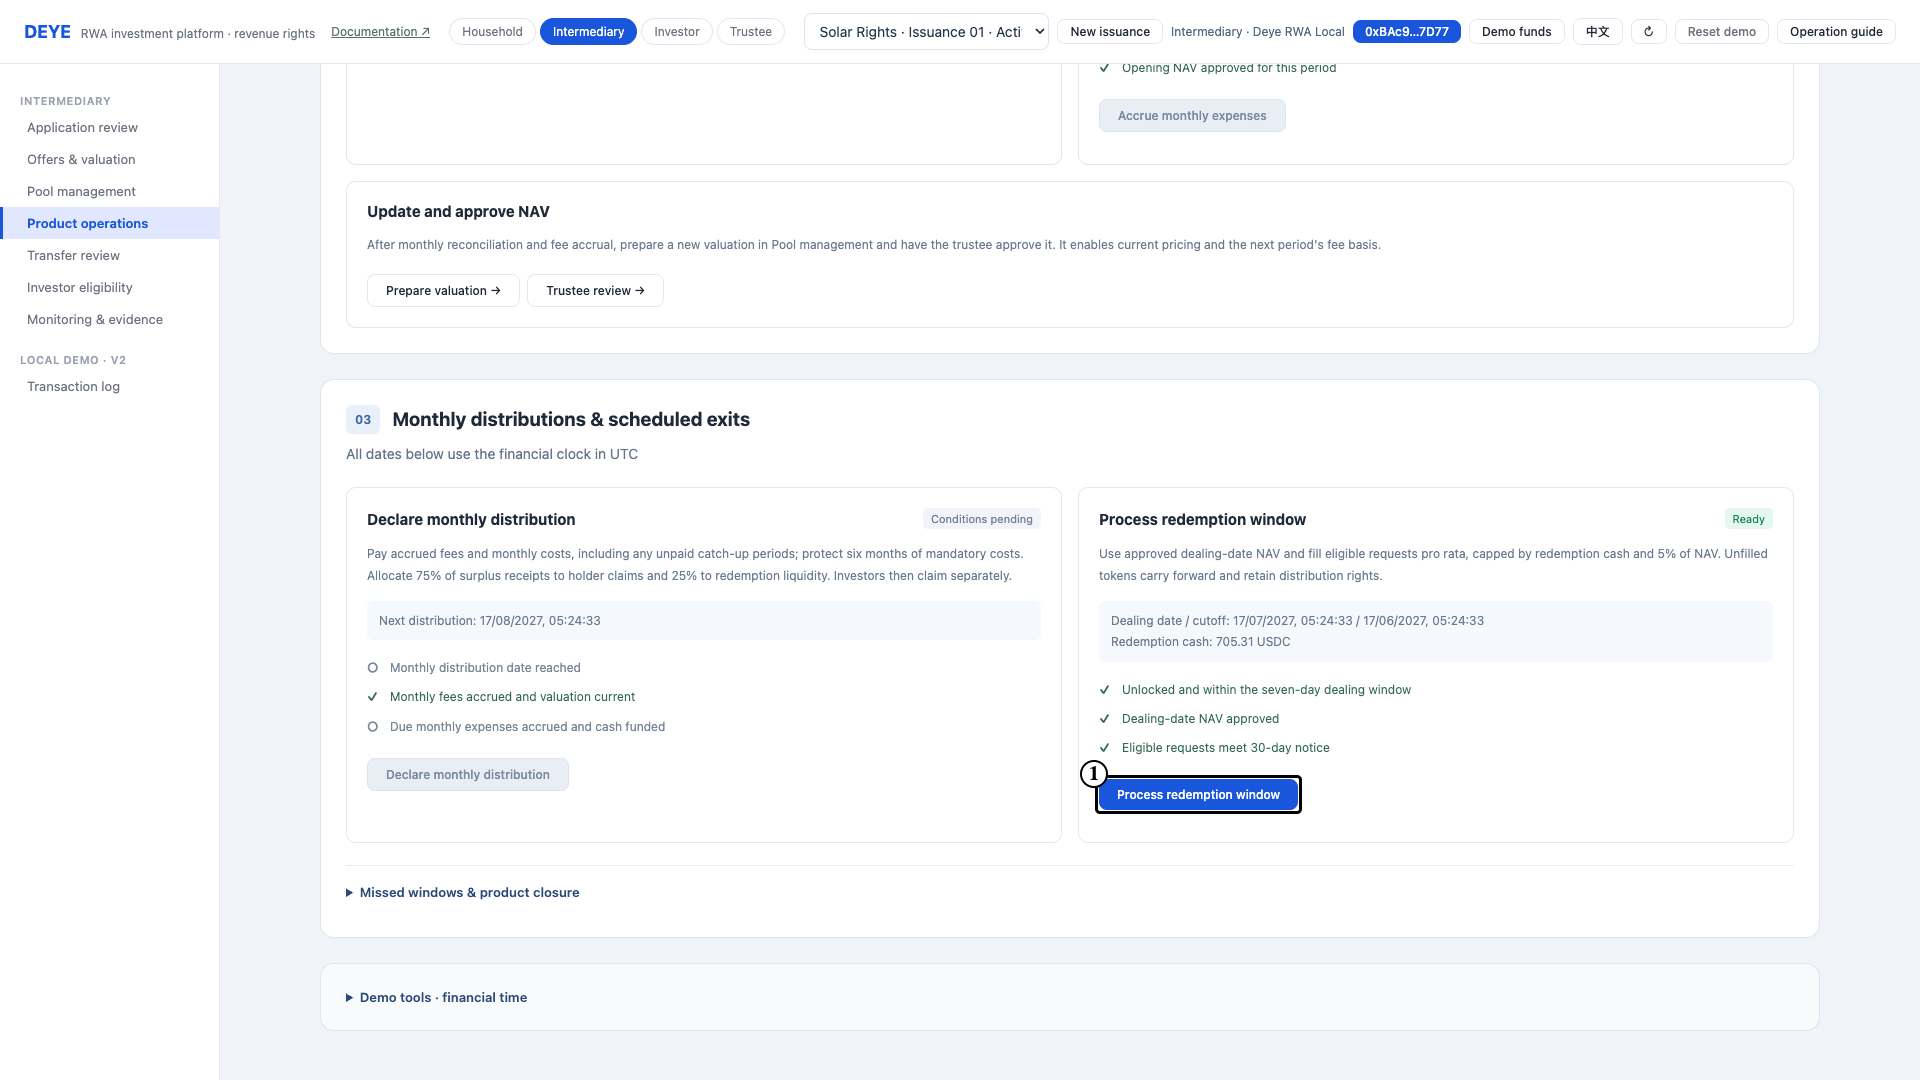
\includegraphics[width=\linewidth,height=.56\textheight,keepaspectratio]{assets/F6.en-context.png}\par Marker 1 identifies the control or information to inspect for this step. Amounts and dates refer to the isolated demonstration.\end{center}
\begin{center}
\includegraphics[width=.7\linewidth,height=1.55cm,keepaspectratio]{assets/F6.en-detail.png}\end{center}
\end{landscape}
\clearpage\begin{landscape}
\subsection{F7 Cancellation of the unfilled request}
\label{step:F7}
This step is performed by Investor. Before the next cutoff, cancel the outstanding unpaid portion of the redemption request. Confirm that these escrowed shares return to the wallet. Already paid and burned shares cannot be cancelled.

After this step, continue holding or submit a later request if appropriate.

\begin{center}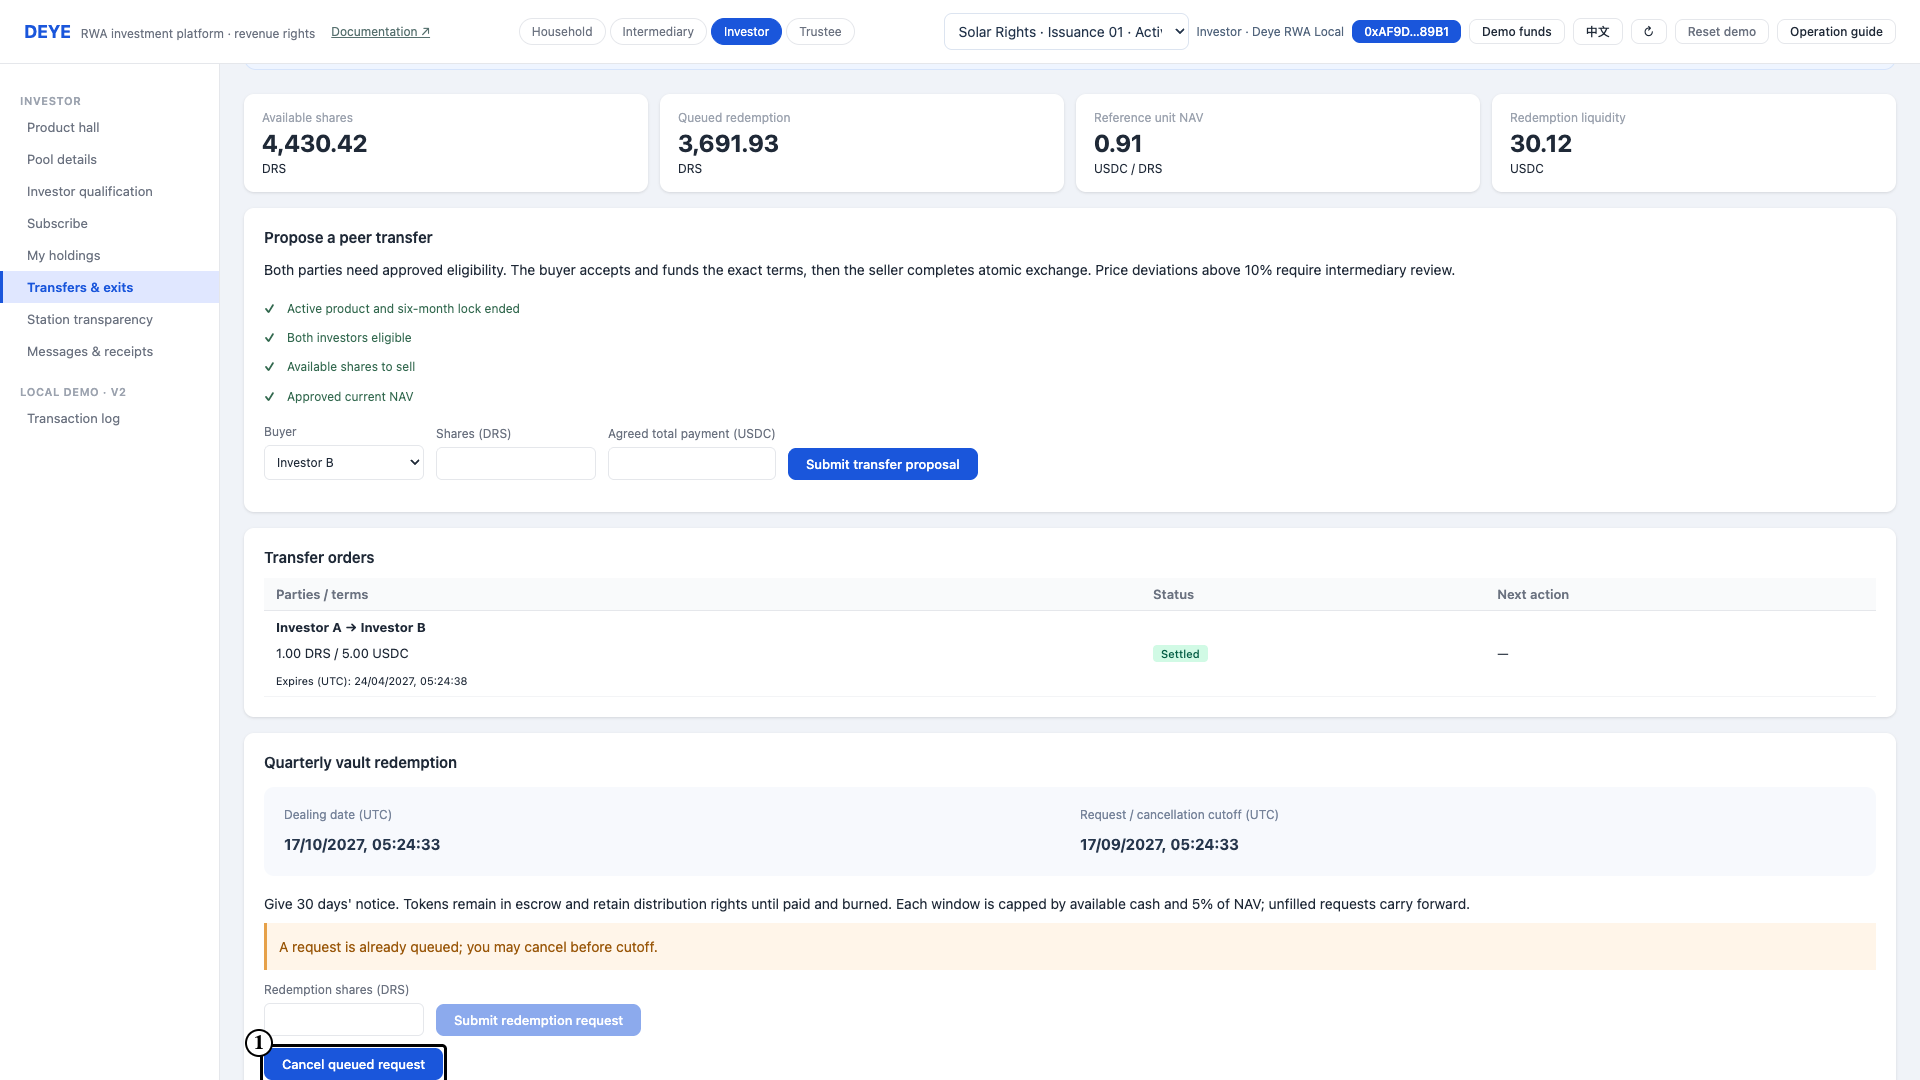
\includegraphics[width=\linewidth,height=.56\textheight,keepaspectratio]{assets/F7.en-context.png}\par Marker 1 identifies the control or information to inspect for this step. Amounts and dates refer to the isolated demonstration.\end{center}
\begin{center}
\includegraphics[width=.7\linewidth,height=1.55cm,keepaspectratio]{assets/F7.en-detail.png}\end{center}
\end{landscape}
\clearpage\begin{landscape}
\section{Servicing cases and trustee intervention}
\subsection{G1 Servicing case creation}
\label{step:G1}
This step is performed by Intermediary. Open Monitoring and evidence and document the reason, supporting evidence and proposed collection-recipient change. Create the case and inspect its fixed ownership snapshot. Ordinary forecast underperformance is not automatically a household default.

After this step, investors review the case and may support it using snapshot weights.

\begin{center}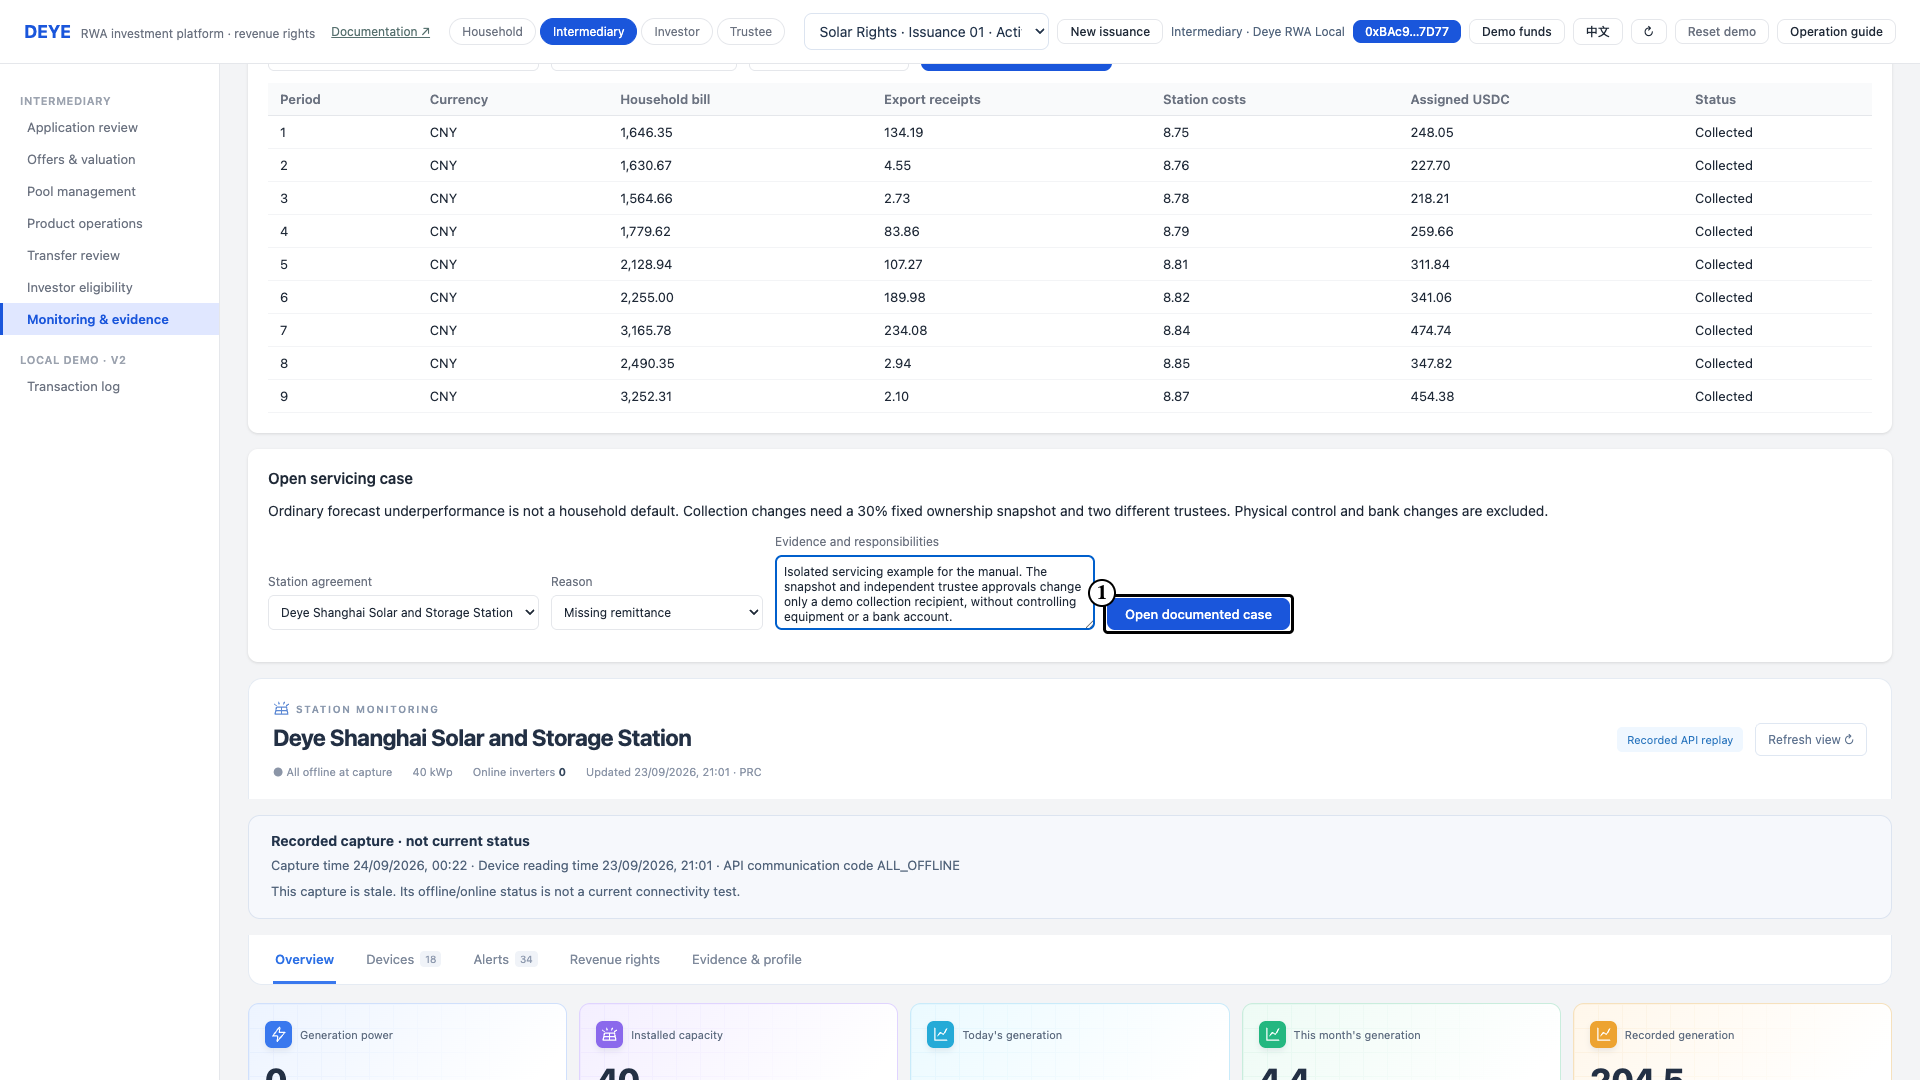
\includegraphics[width=\linewidth,height=.44\textheight,keepaspectratio]{assets/G1.en-context.png}\par Marker 1 identifies the control or information to inspect for this step. Amounts and dates refer to the isolated demonstration.\end{center}
\begin{center}
\includegraphics[width=.7\linewidth,height=1.55cm,keepaspectratio]{assets/G1.en-detail.png}\end{center}
\end{landscape}
\clearpage\begin{landscape}
\subsection{G2 Snapshot-weighted support}
\label{step:G2}
This step is performed by Investor. Read the case and the proposed recipient, then confirm support with the investor wallet. The contract uses the fixed snapshot and requires 30\% support before trustee action. Later transfers cannot create duplicate voting weight.

After this step, trustee A independently reviews the eligible case.

\begin{center}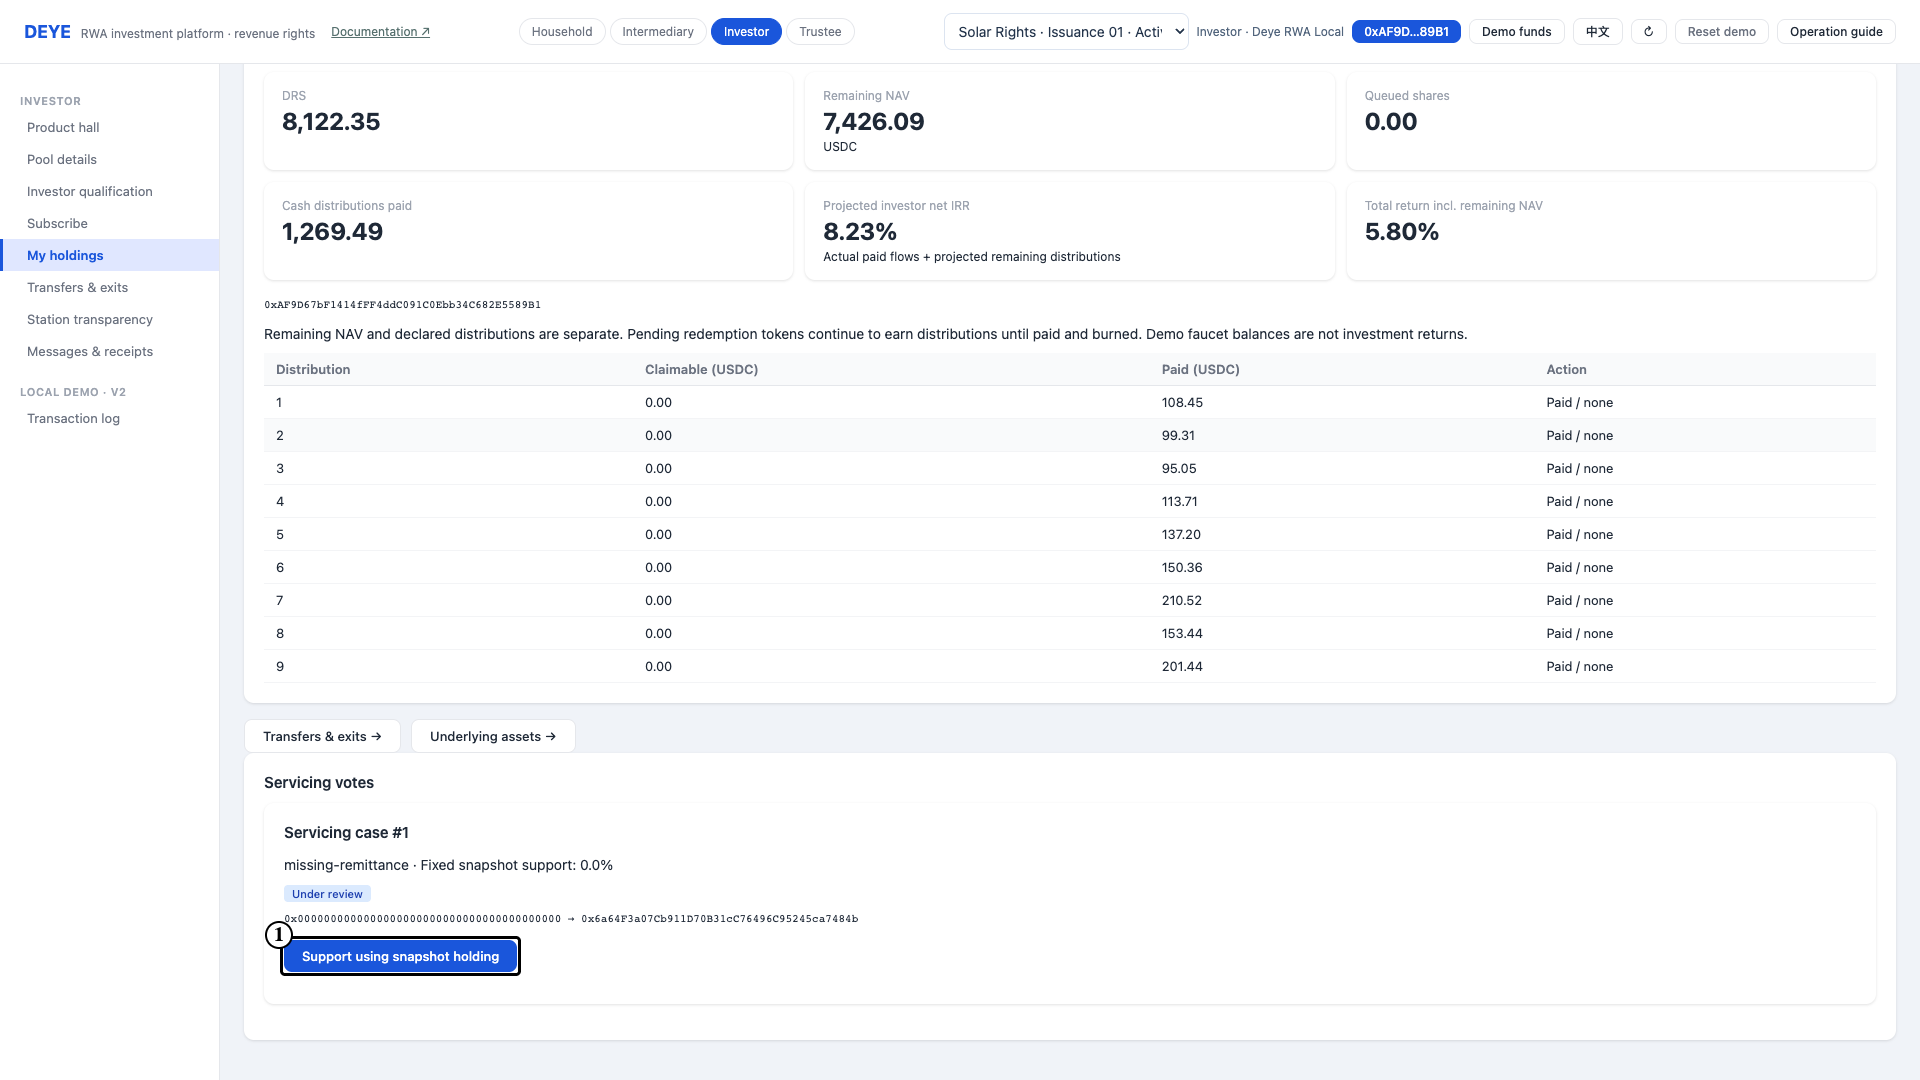
\includegraphics[width=\linewidth,height=.56\textheight,keepaspectratio]{assets/G2.en-context.png}\par Marker 1 identifies the control or information to inspect for this step. Amounts and dates refer to the isolated demonstration.\end{center}
\begin{center}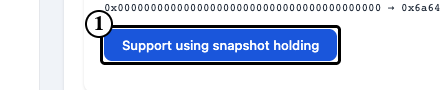
\includegraphics[width=.7\linewidth,height=1.55cm,keepaspectratio]{assets/G2.en-detail.png}\end{center}
\end{landscape}
\clearpage\begin{landscape}
\subsection{G3 First trustee approval}
\label{step:G3}
This step is performed by Trustee A. Open the case, check evidence, snapshot support and recipient, then approve with trustee A's wallet. The contract records this distinct address but does not yet execute the recipient change.

After this step, trustee B performs a separate review of the same case.

\begin{center}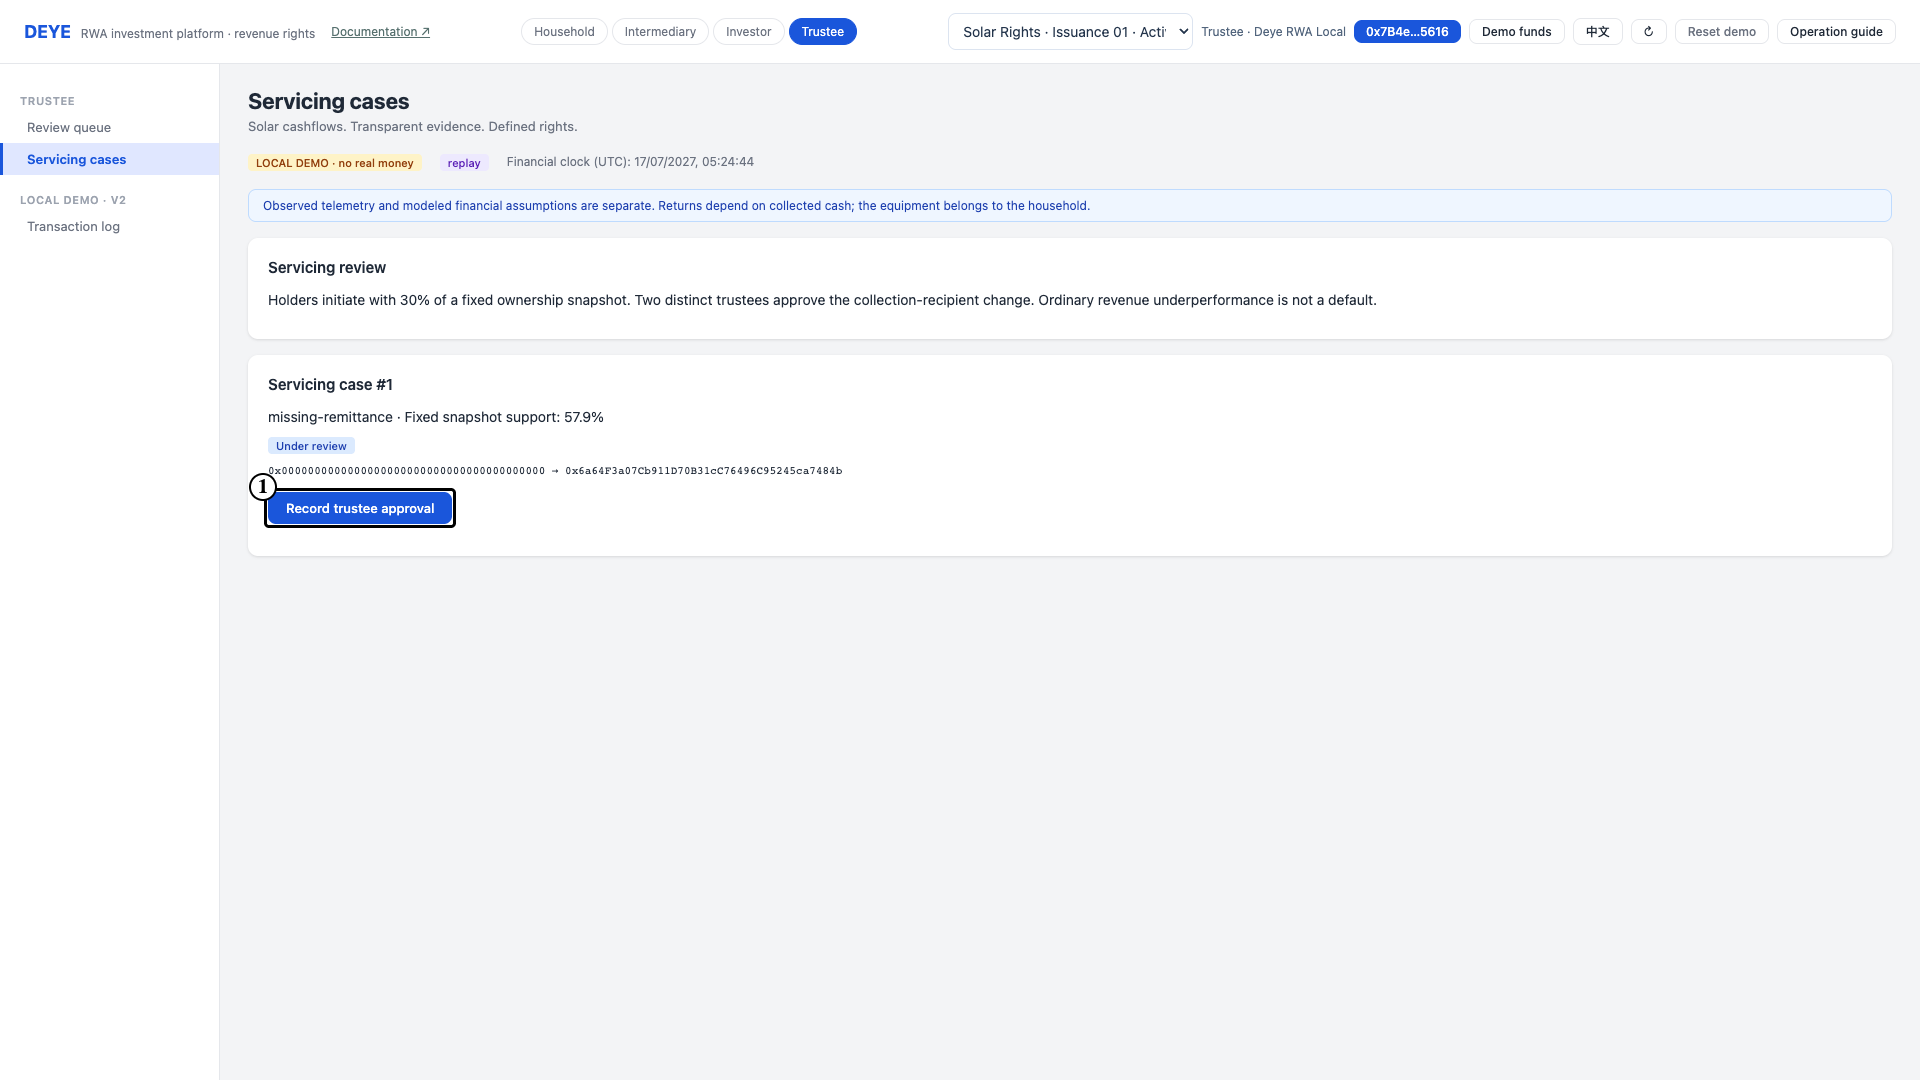
\includegraphics[width=\linewidth,height=.56\textheight,keepaspectratio]{assets/G3.en-context.png}\par Marker 1 identifies the control or information to inspect for this step. Amounts and dates refer to the isolated demonstration.\end{center}
\begin{center}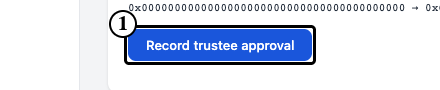
\includegraphics[width=.7\linewidth,height=1.55cm,keepaspectratio]{assets/G3.en-detail.png}\end{center}
\end{landscape}
\clearpage\begin{landscape}
\subsection{G4 Second trustee approval and execution}
\label{step:G4}
This step is performed by Trustee B. Switch to trustee B's configured wallet and sign in again. Review the same case independently and approve it. Two different trustee addresses are required to authorize the demo collection-recipient change, which does not control equipment or a real bank account.

After this step, the intermediary checks execution and continues servicing.

\begin{center}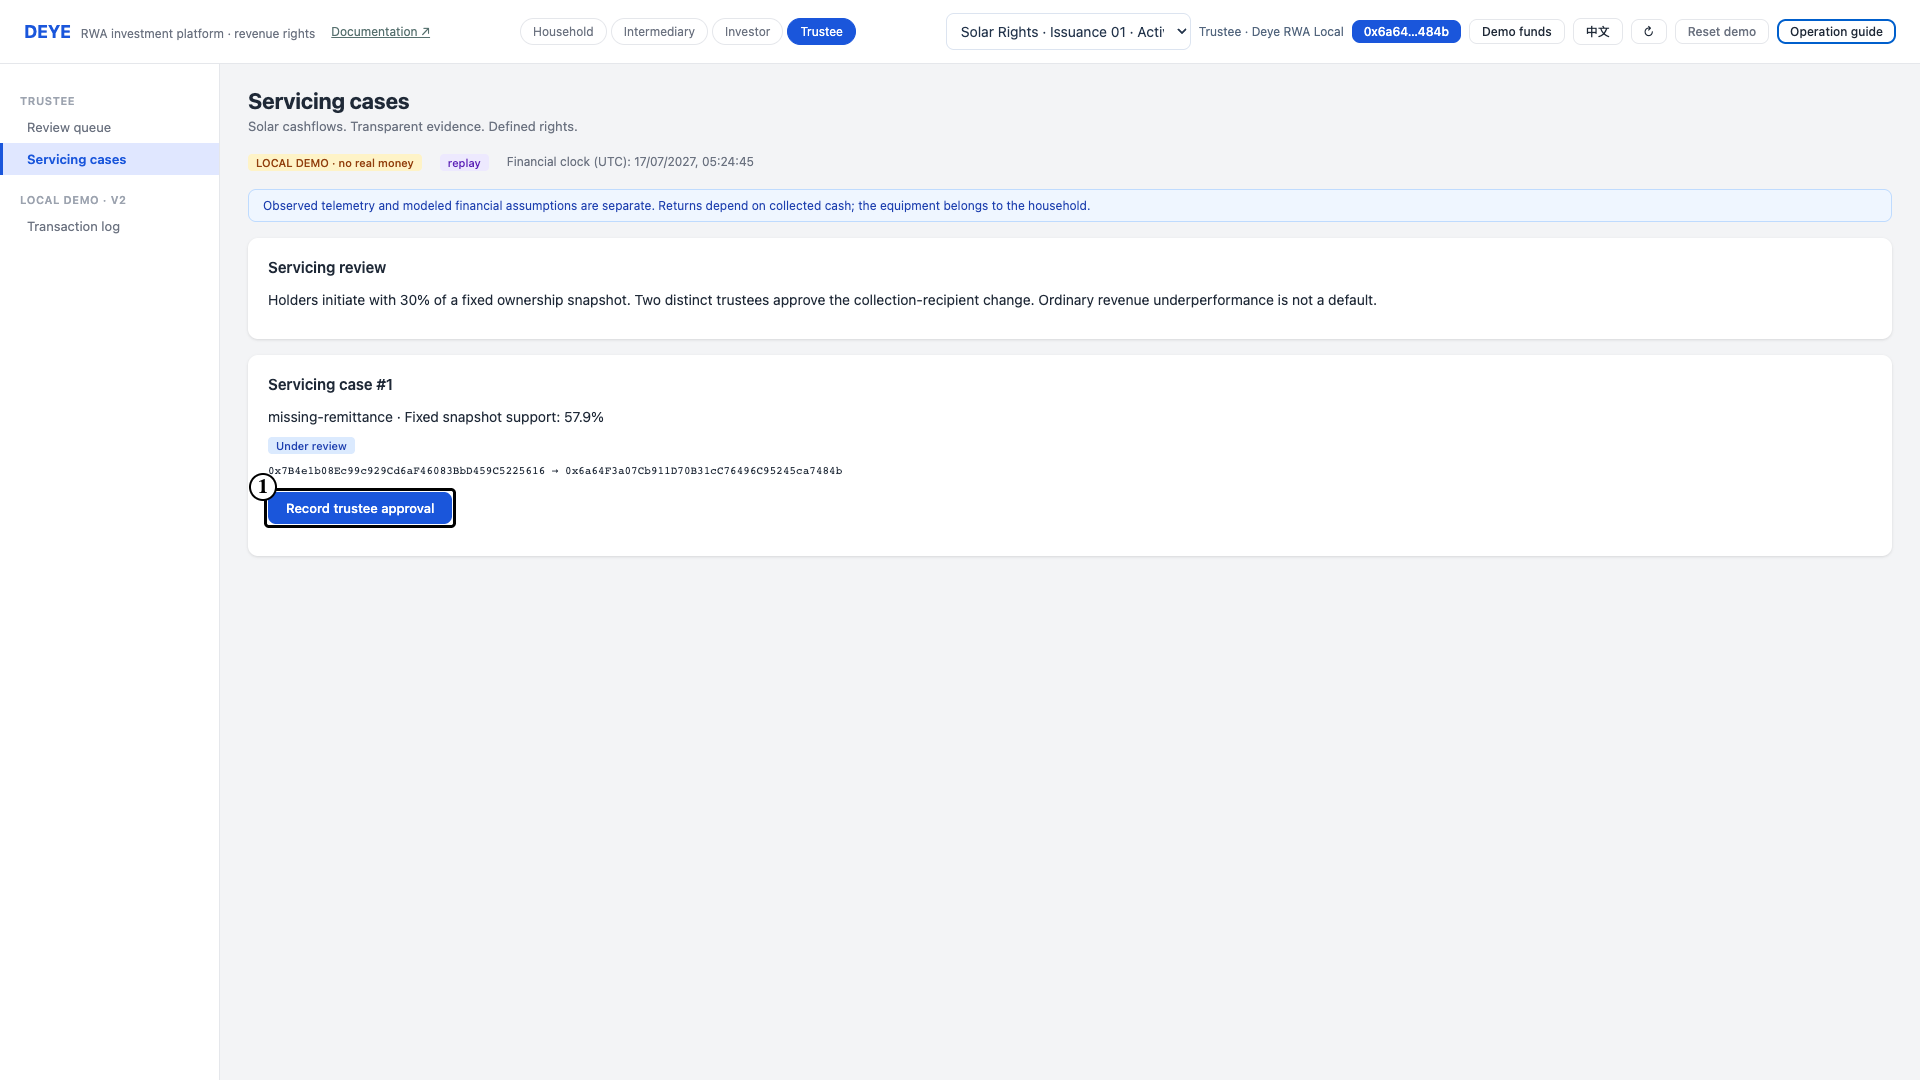
\includegraphics[width=\linewidth,height=.56\textheight,keepaspectratio]{assets/G4.en-context.png}\par Marker 1 identifies the control or information to inspect for this step. Amounts and dates refer to the isolated demonstration.\end{center}
\begin{center}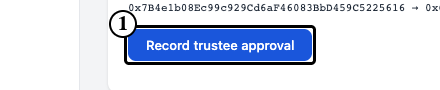
\includegraphics[width=.7\linewidth,height=1.55cm,keepaspectratio]{assets/G4.en-detail.png}\end{center}
\end{landscape}
\clearpage\begin{landscape}
\section{Expiry, closure and credential release}
\subsection{H1 Product closure at rights expiry}
\label{step:H1}
This step is performed by Intermediary. After all 60 service months, reconcile receivables, accrued liabilities and distributions, then obtain the final required valuation approval. Confirm Close product when every condition is satisfied. Remaining cash becomes a final distribution rather than an invented repayment of original principal.

After this step, investors claim remaining amounts and the owner retrieves the station credential.

\begin{center}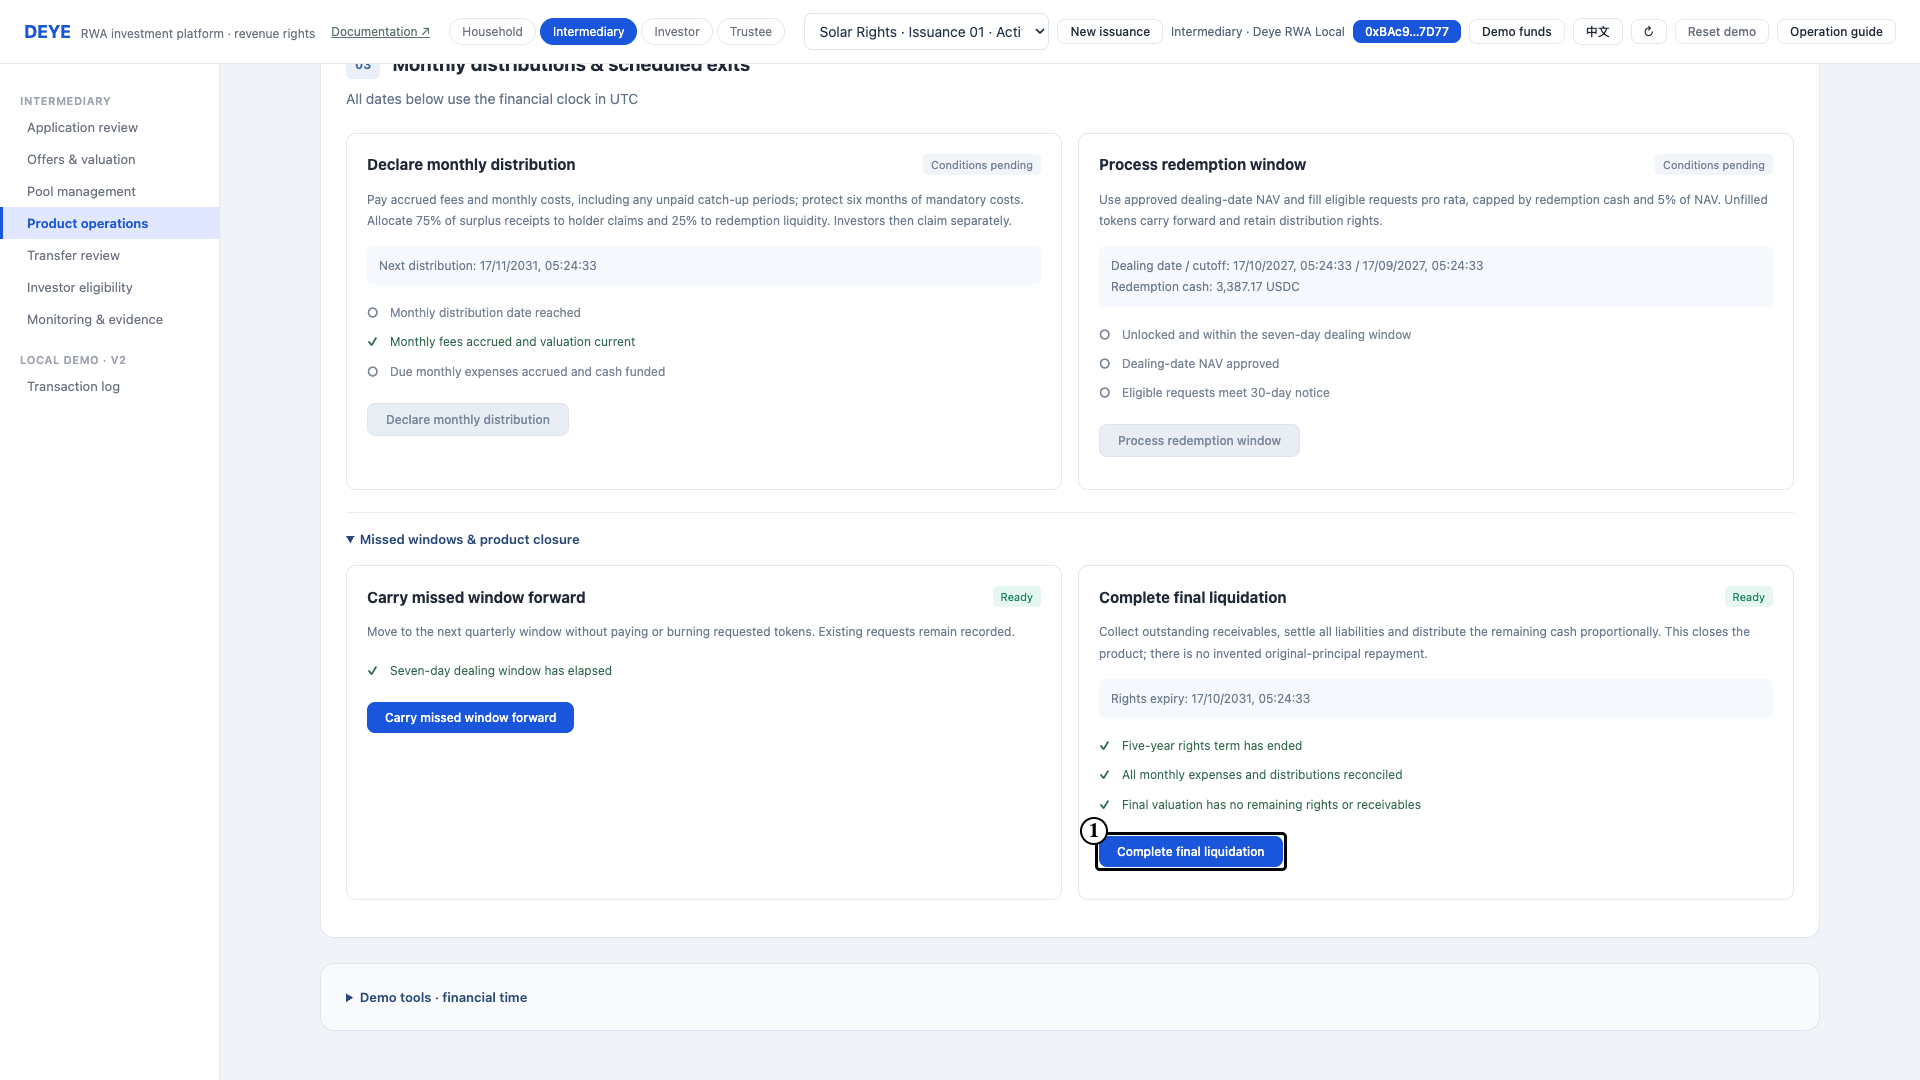
\includegraphics[width=\linewidth,height=.44\textheight,keepaspectratio]{assets/H1.en-context.png}\par Marker 1 identifies the control or information to inspect for this step. Amounts and dates refer to the isolated demonstration.\end{center}
\begin{center}
\includegraphics[width=.7\linewidth,height=1.55cm,keepaspectratio]{assets/H1.en-detail.png}\end{center}
\end{landscape}
\clearpage\begin{landscape}
\subsection{H2 Final and outstanding distribution claims}
\label{step:H2}
This step is performed by Each investor. Review every unpaid distribution in My holdings and claim the amounts belonging to this wallet. Check the confirmed USDC transfers. Previously paid distributions are not paid again, and a remaining historical DRS balance does not extend expired revenue rights.

After this step, the owner completes station credential release.

\begin{center}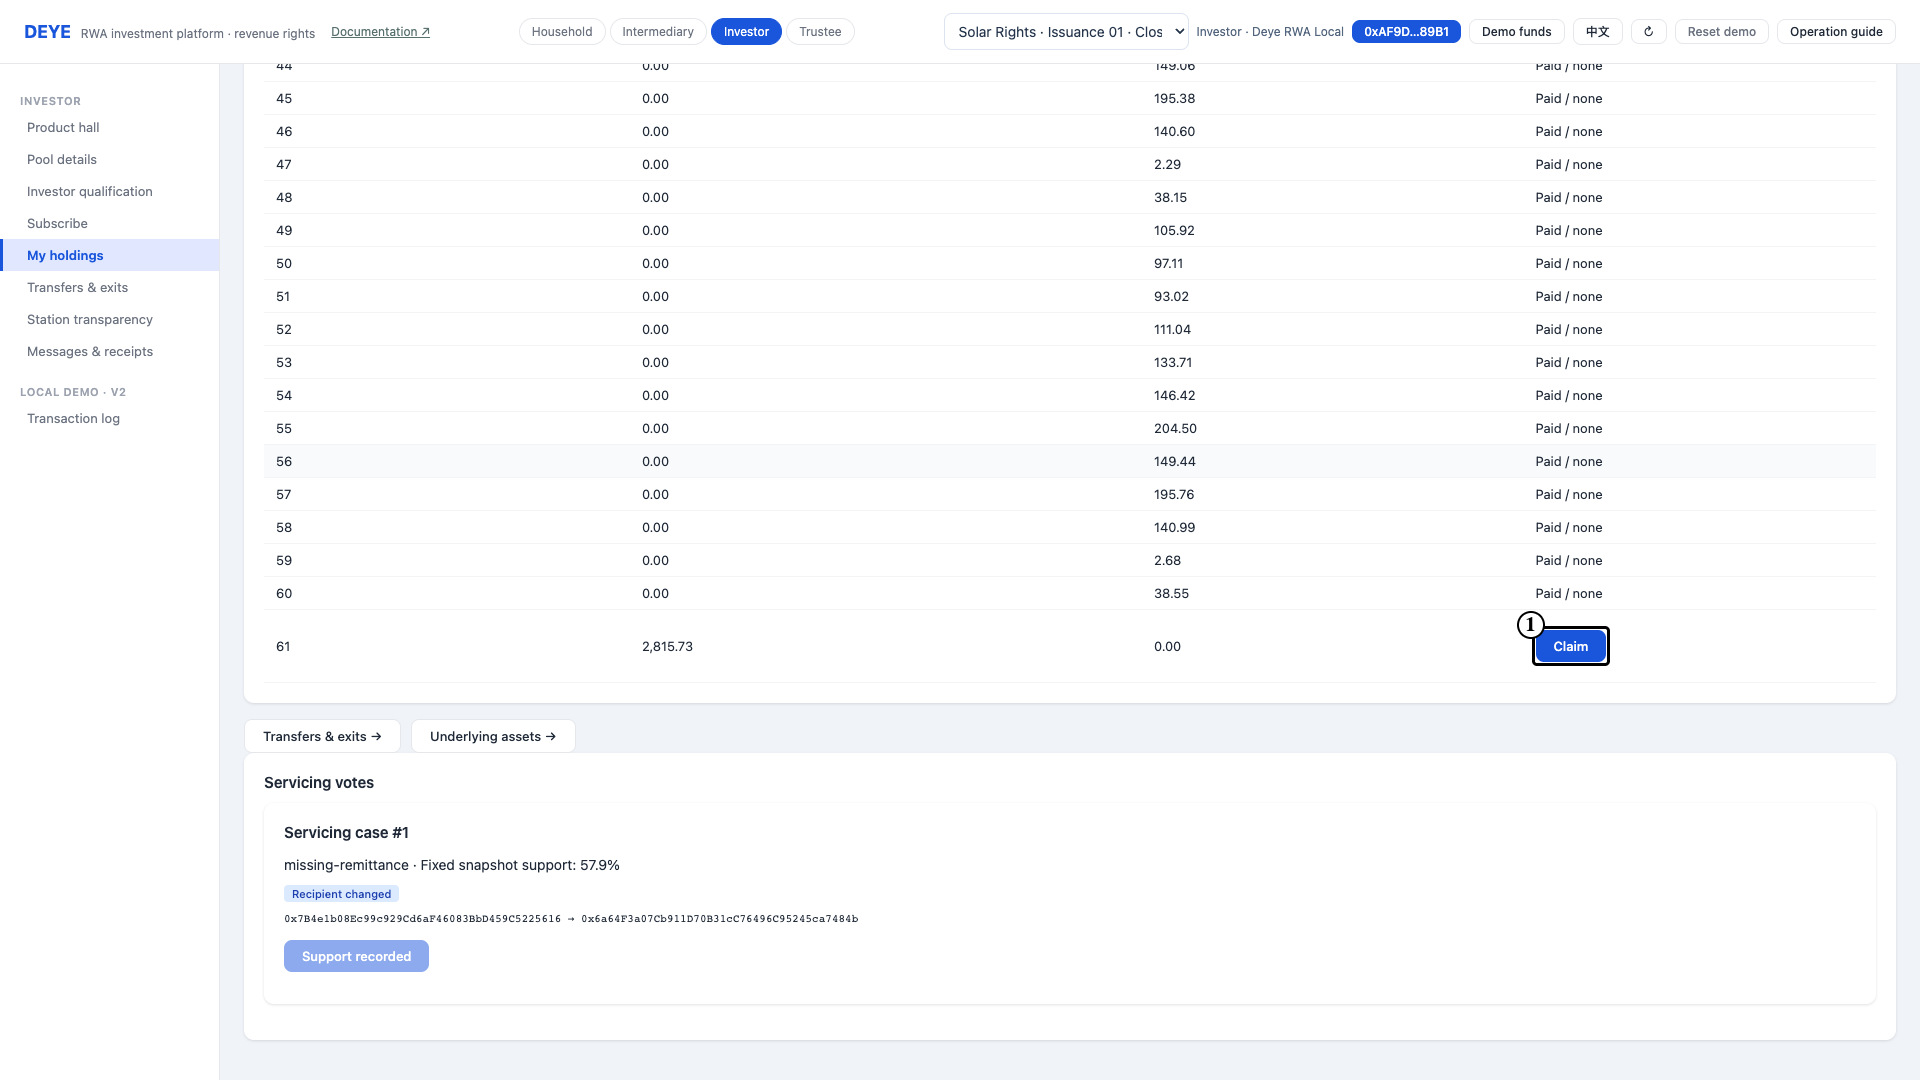
\includegraphics[width=\linewidth,height=.56\textheight,keepaspectratio]{assets/H2.en-context.png}\par Marker 1 identifies the control or information to inspect for this step. Amounts and dates refer to the isolated demonstration.\end{center}
\begin{center}
\includegraphics[width=.7\linewidth,height=1.55cm,keepaspectratio]{assets/H2.en-detail.png}\end{center}
\end{landscape}
\clearpage\begin{landscape}
\subsection{H3 Station credential release}
\label{step:H3}
This step is performed by Owner. Open the expired agreement's release task after product closure. Confirm the release transaction and check that the station NFT returns from the vault to the owner. Equipment ownership remained with the owner throughout the agreement.

After this step, the product lifecycle is complete and its transaction history remains queryable.

\begin{center}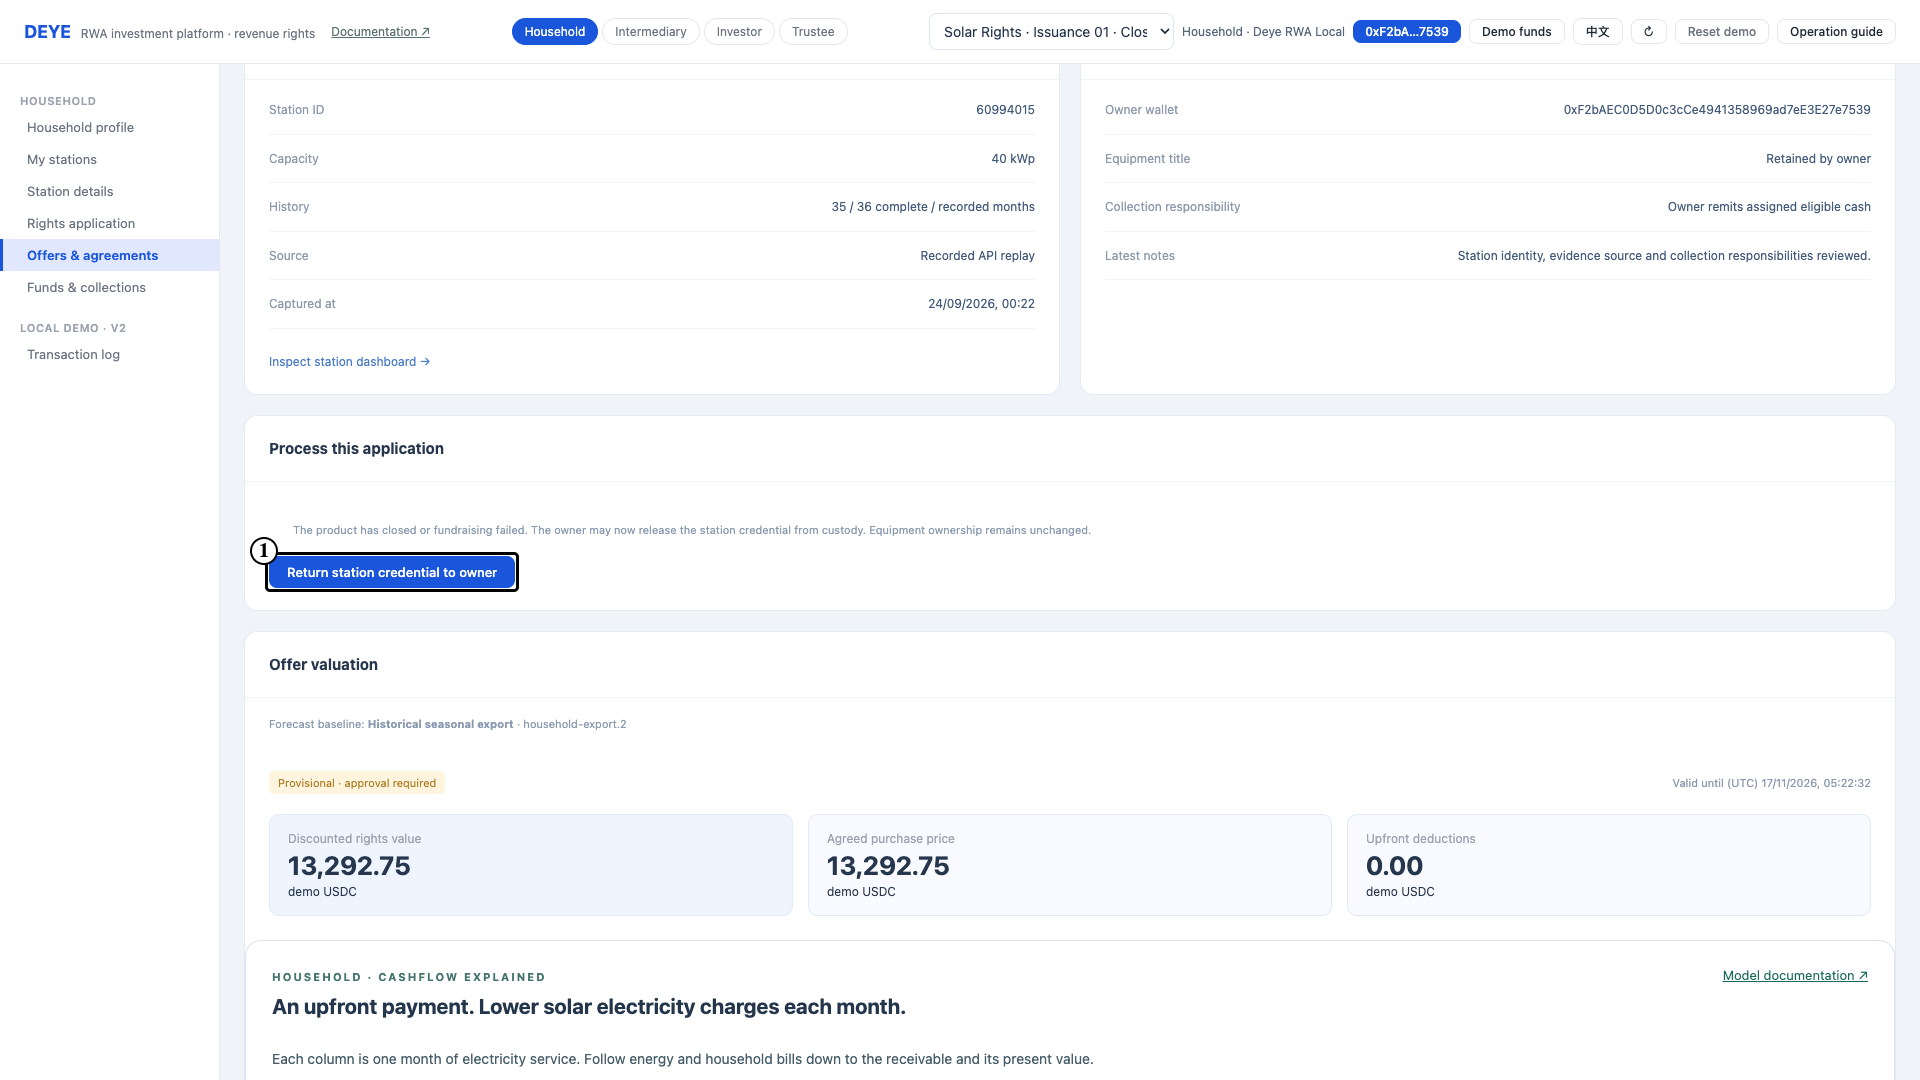
\includegraphics[width=\linewidth,height=.56\textheight,keepaspectratio]{assets/H3.en-context.png}\par Marker 1 identifies the control or information to inspect for this step. Amounts and dates refer to the isolated demonstration.\end{center}
\begin{center}
\includegraphics[width=.7\linewidth,height=1.55cm,keepaspectratio]{assets/H3.en-detail.png}\end{center}
\end{landscape}
\clearpage\section{Cashflow calculations and valuation}
The forecast uses up to 36 available historical months to form calendar-month seasonal baselines, then applies degradation, availability, export behavior and tariff schedules. Fewer than 12 complete months requires a labeled provisional estimate and review. Imbalanced generation and export samples require investigation rather than silently capping export at 100\% and treating the result as valid self-use.

\[S_t=\max(G_t-E_t,0)\,q_t,\qquad B_t=S_t\,p^{grid}_t\,d_t.\]
G denotes forecast generation, E is validated eligible export and q is the self-use delivery factor. S is delivered self-use and B is the owner’s electricity payment at discount factor d. The grid-price comparison is S times the grid tariff. The difference is the saving on this delivered solar energy, not a claim that the owner’s entire grid bill falls by the same percentage.

\[C_t=(B_t+E_t p^{export}_t-K_t)\,f_t\,a_t,\qquad V_0=\sum_{t=1}^{60}\frac{\widehat C_t}{(1+r)^{\tau_t/12}}.\]
K represents agreed station costs borne by the rights, f is the demo FX conversion into USDC and a is the signed assignment proportion. New agreements default to 100\% assignment, with the owner retaining a benefit through the discounted tariff. Discounting uses expected cash-collection dates, so tau includes receipt delays. The default 10\% nominal annual discount rate is a pricing assumption, not a promised return, and 6\% and 14\% sensitivities are also shown.

\clearpage\begin{landscape}
\subsection{Owner cashflow timeline for the first three periods}
\begin{center}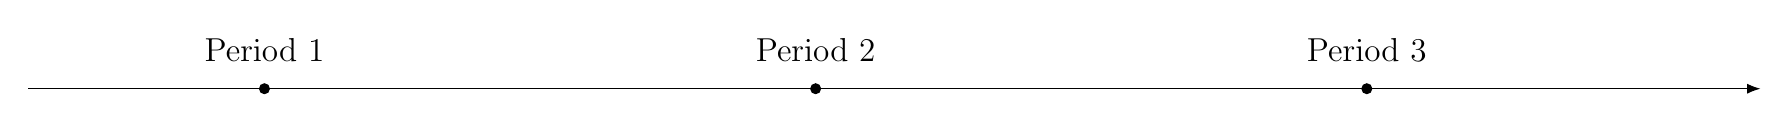
\begin{tikzpicture}[>=Latex]\draw[->](0,0)--(22,0);
\fill(3,0)circle(2pt);\node[above]at(3,.2){Period 1};
\fill(10,0)circle(2pt);\node[above]at(10,.2){Period 2};
\fill(17,0)circle(2pt);\node[above]at(17,.2){Period 3};
\end{tikzpicture}\end{center}\begin{center}\begin{tabular}{L{10cm}rrr}\toprule Calculation & Period 1 & Period 2 & Period 3\\\midrule
Generation kWh & 3,861.20 & 4,307.49 & 3,732.04\\
Export kWh & 279.01 & 308.98 & 67.61\\
Delivered self-use kWh & 3,223.97 & 3,598.66 & 3,297.99\\
Grid-price comparison CNY & 1,934.38 & 2,159.19 & 1,978.80\\
Owner electricity payment CNY & 1,547.51 & 1,727.36 & 1,583.04\\
Owner saving CNY & 386.88 & 431.84 & 395.76\\
Export income CNY & 97.65 & 108.14 & 23.66\\
Station costs CNY & 8.75 & 8.76 & 8.78\\
Assigned net receivable USDC & 229.10 & 255.74 & 223.71\\
Discounted present value USDC & 225.48 & 249.68 & 216.64\\
\bottomrule\end{tabular}\end{center}
These values come from one isolated product report and are modeled examples. The full report covers 60 periods. Owner bills, export income and costs are calculated separately and discounted at their expected collection times.

\end{landscape}
\clearpage\begin{landscape}
\subsection{Investor cashflow timeline for the first three months}
\begin{center}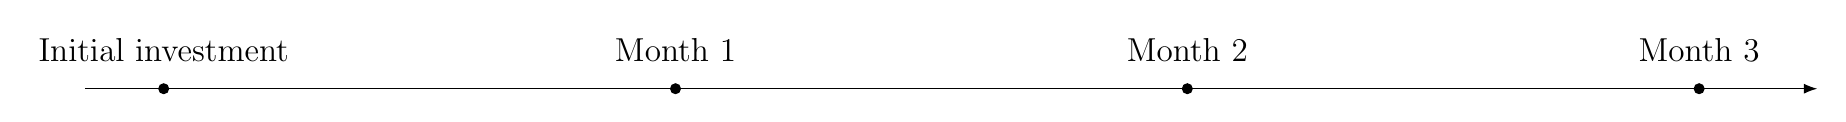
\begin{tikzpicture}[>=Latex]\draw[->](0,0)--(22,0);
\fill(1.0,0)circle(2pt);\node[above]at(1.0,.2){Initial investment};
\fill(7.5,0)circle(2pt);\node[above]at(7.5,.2){Month 1};
\fill(14.0,0)circle(2pt);\node[above]at(14.0,.2){Month 2};
\fill(20.5,0)circle(2pt);\node[above]at(20.5,.2){Month 3};
\end{tikzpicture}\end{center}\begin{center}\begin{tabular}{L{11cm}rrr}\toprule Calculation & Month 1 & Month 2 & Month 3\\\midrule
Forecast cash collected USDC & 0.00 & 229.10 & 255.74\\
Accrued annual-fee portion USDC & 6.04 & 6.09 & 6.06\\
Mandatory monthly pool costs USDC & 1.00 & 1.00 & 1.00\\
Pool distribution USDC & 0.00 & 166.51 & 186.51\\
Pool cash after distribution USDC & 1,469.93 & 1,525.43 & 1,587.60\\
Forecast payout per 1,000 USDC & 0.00 & 11.27 & 12.63\\\bottomrule\end{tabular}\end{center}
The vault automatically retains 10\% of initial subscription cash and uses the balance to purchase rights. Monthly declarations require the relevant collections, expenses and valuation conditions and do not guarantee a positive payout each month. Investors must still claim. Monthly distribution does not remove the six-month transfer lock or change quarterly redemption windows.

Investor NAV consists of cash, collectible receivables and remaining rights, less liabilities and applicable future costs. Declared distributions are separated from dealing NAV to prevent double counting. Projected net IRR uses the initial investment, expected distributions and final cash. Assess paid cash, remaining NAV and total return together.

\end{landscape}
\clearpage\section{On-chain record reconciliation}
For each monthly invoice, reconcile BillPublished, HouseholdPaid, ExportFunded and ReceiptConfirmed separately. Household payment must come from the named owner to the product billing contract for the invoiced amount. The intermediary signs receipt confirmation. Check net proceeds into the vault and station costs paid once. Paid but unconfirmed amounts remain in the billing contract, separate from vault cash.

For NFT minting, check the station token ID and owner. For approval, check the authorized vault. For admission, check custody, agreement digest and purchase price. For valuation, check report digest, reviewer and validity. Distinguish subscription transfers from settlement, and reconcile cumulative escrow, issued DRS, owner payment and retained cash.

\begin{center}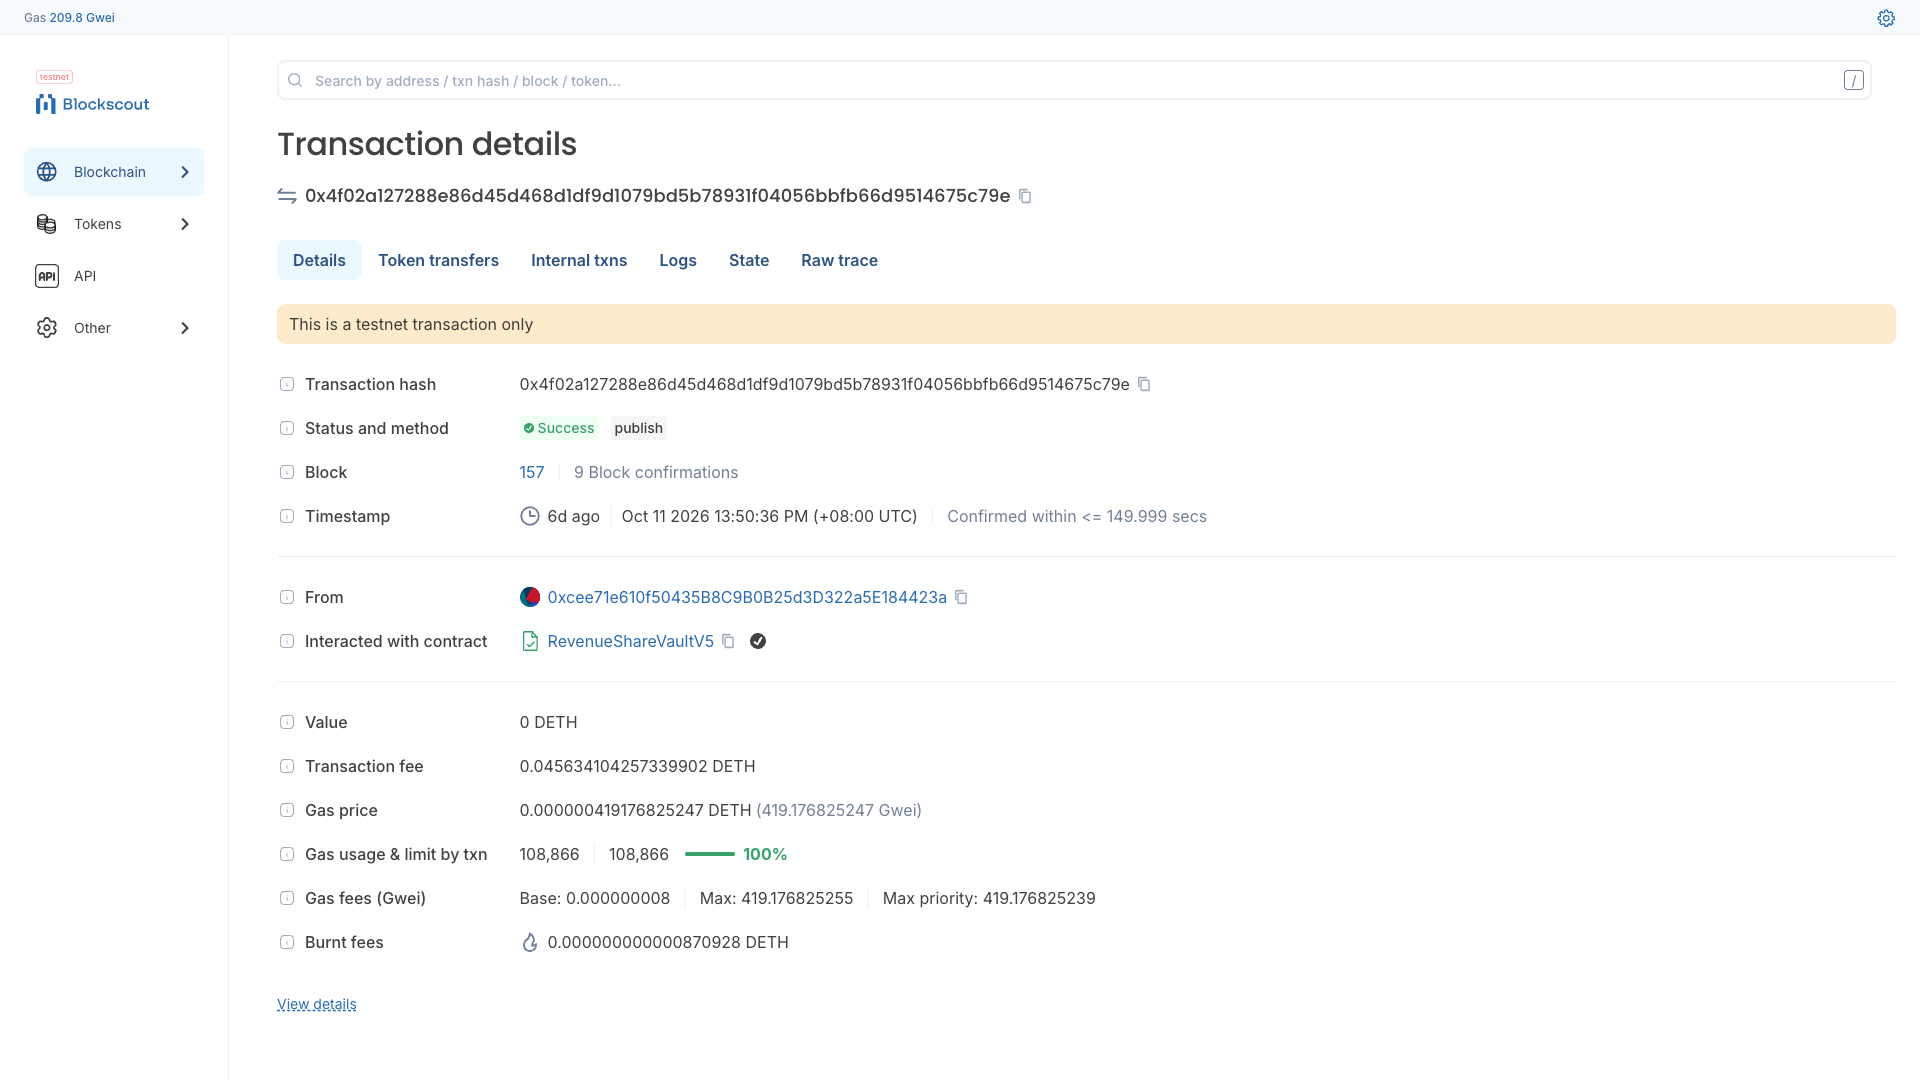
\includegraphics[width=\linewidth,height=.4\textheight,keepaspectratio]{assets/explorer-transaction.en.png}\par Explorer transaction example. Check execution status, sender, target contract and block.\end{center}
\clearpage
Declaration and claim are different transactions. Declaration creates an entitlement, while claiming transfers USDC to the investor. A peer settlement should contain both the DRS and USDC legs. A redemption should reconcile the fill, payment, burn and remaining escrow. A servicing case should show its snapshot, support weight and two distinct approval addresses.

\begin{center}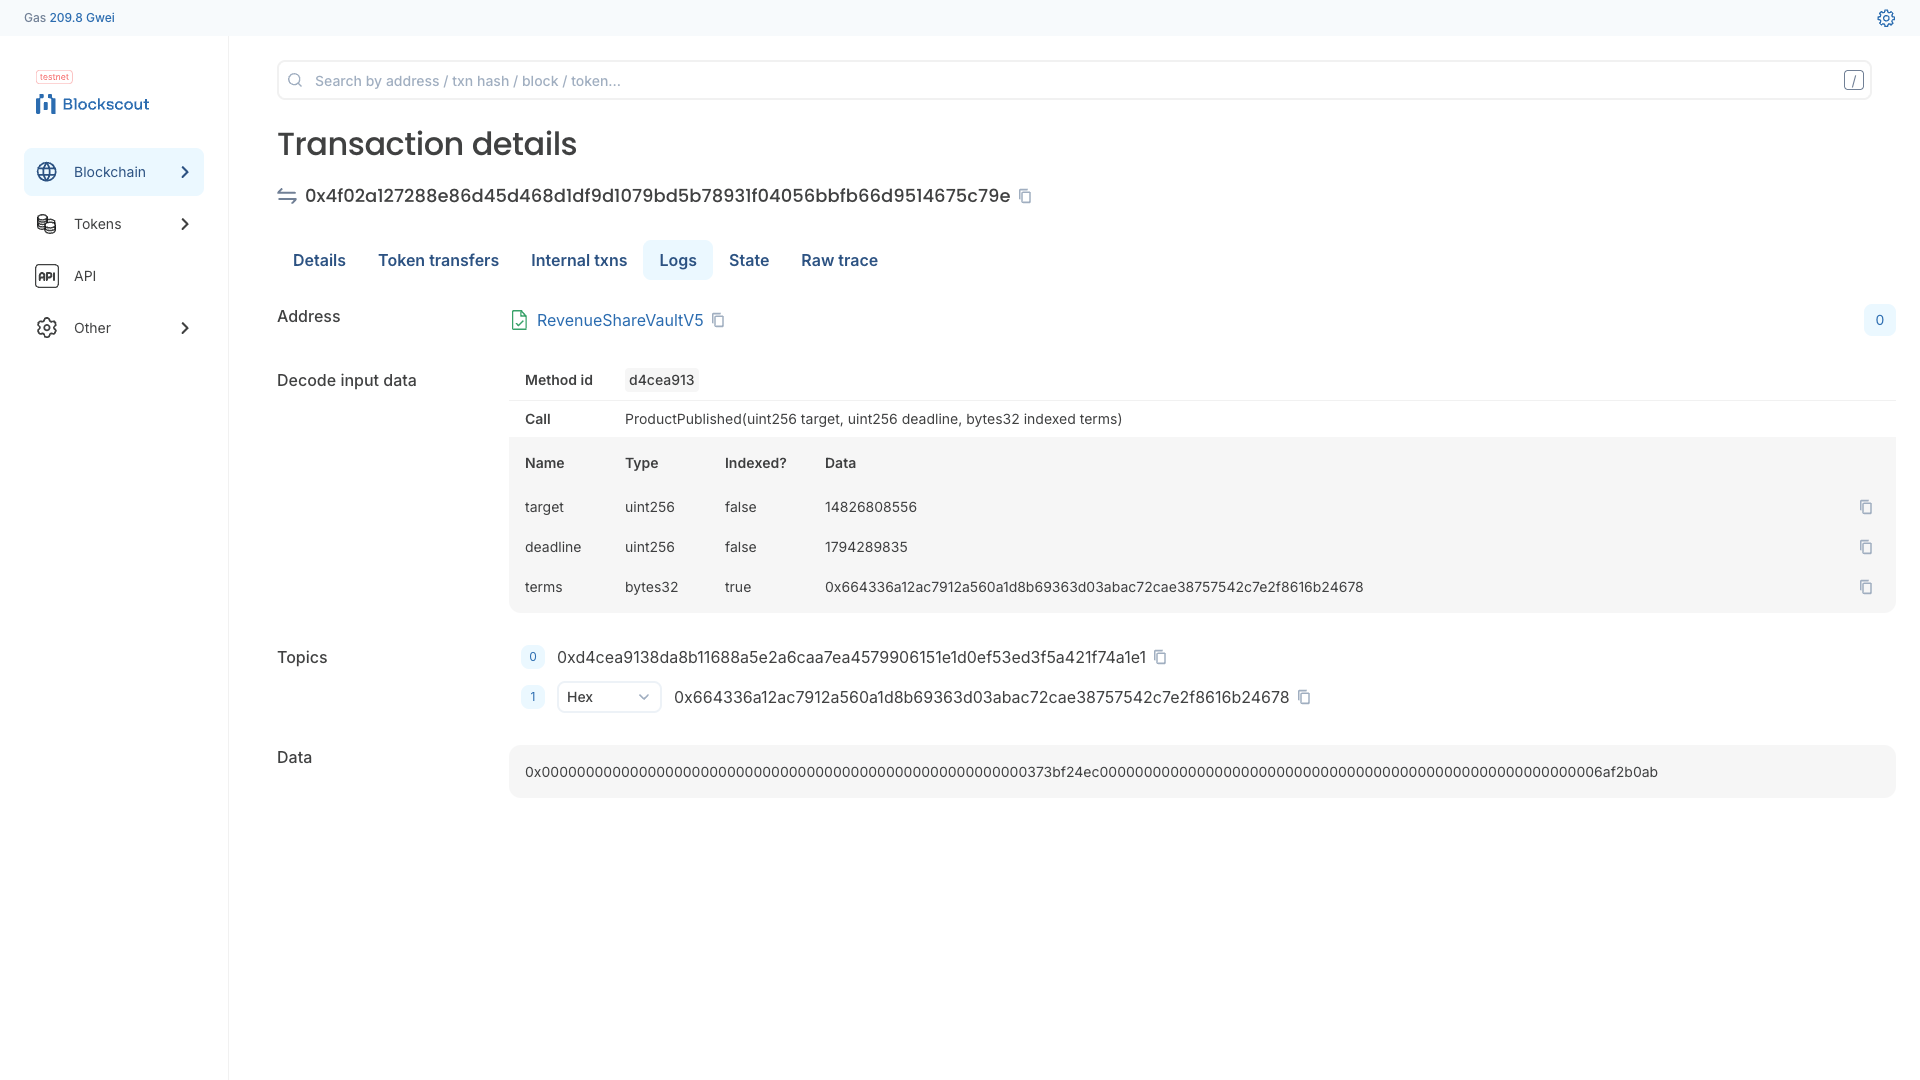
\includegraphics[width=\linewidth,height=.42\textheight,keepaspectratio]{assets/explorer-events.en.png}\par Events and token-record example. A digest links the off-chain record without storing the full underlying material on-chain.\end{center}
\clearpage\section{Troubleshooting and test boundaries}
\subsection{Wallet or role mismatch}
Check the full address, Chain ID and selected role. Switch the wallet account and sign in again with the intended role. Repeated role-button clicks do not grant permissions.

\subsection{Insufficient settlement funding}
The contract automatically retains 10\% as initial cash. Minimum funding typically covers the purchase price divided by 90\%. Add the displayed shortfall and have the intermediary review the new total rather than editing accounting records.

\subsection{Missing valuation or fee prerequisites}
Use Locate operation to open the specific remedy. The intermediary reprepares an expired or changed report and the trustee approves it. Reaching the cutoff does not itself approve NAV.

\subsection{Distribution or balance not updated}
Check whether the current period was declared, then distinguish claimable amounts from paid history. Wallet USDC, escrow and investment NAV are separate. If confirmation precedes indexing, retain the hash and refresh later.

\subsection{Rejection, pending transactions and recovery}
After rejection, review and retry the original action. If a hash exists, inspect its receipt before sending another payment. Refresh and backend restart should recover the original operation. A complete test-chain rebuild requires the operator to notify users about clearing stale test-network transaction caches.

\subsection{Remote environment unavailable}
The GitHub homepage remains readable, but the app, RPC and Blockscout depend on the Mac, Docker and tunnels. The operator first checks unified:status, then checks the two backend services and tunnels separately. If a tunnel address changes, update the unified entry and GitHub static configuration.

\end{document}
